%  Clam AntiVirus Bytecode Compiler: User Manual
%
%  Copyright (C) 2009 Sourcefire, Inc.
%  Author: Török Edvin <edwin@clamav.net>
%
%  This program is free software; you can redistribute it and/or modify
%  it under the terms of the GNU General Public License as published by
%  the Free Software Foundation; either version 2 of the License, or
%  (at your option) any later version.
%
%  This program is distributed in the hope that it will be useful,
%  but WITHOUT ANY WARRANTY; without even the implied warranty of
%  MERCHANTABILITY or FITNESS FOR A PARTICULAR PURPOSE.  See the
%  GNU General Public License for more details.
%
%  You should have received a copy of the GNU General Public License
%  along with this program; if not, write to the Free Software
%  Foundation, Inc., 51 Franklin Street, Fifth Floor, Boston,
%  MA 02110-1301, USA.

\documentclass[a4paper,titlepage,12pt,english]{book}
\usepackage{lmodern}
\usepackage[T1]{fontenc}
\usepackage{textcomp}
\usepackage{fancyhdr}
\usepackage{longtable}
\usepackage{afterpage}
\usepackage{ifthen}
\usepackage{ifpdf}
\usepackage{titlesec}
\usepackage{microtype}
\usepackage[footnotesize,bf,justification=centering]{caption}
\usepackage[usenames, dvipsnames]{color}
%%% general setup
\usepackage[english]{babel}
\usepackage[utf8x]{inputenc}
\usepackage[perpage]{footmisc}
\usepackage{nomencl}
\usepackage{boxedminipage}
\usepackage{float}
\usepackage{algorithmic}
\usepackage{subfig}
\usepackage{moreverb}
\usepackage{listings}
\usepackage{prettyref}
\usepackage{url}
\usepackage{doxygen}
\usepackage{makeidx}
\usepackage{xcolor}
%\makeindex
\lstset{language=[GNU]C++}
\lstset{escapeinside={(*@}{@*)}}
\lstset{numbers=left, numberstyle=\tiny, stepnumber=2,numbersep=5pt,
  extendedchars=true,keywordstyle=\color{blue},
  stringstyle=\color{green!30!black}\ttfamily,
  commentstyle=\rmfamily,
  showspaces=false,showtabs=false,
  basicstyle=\footnotesize\ttfamily, breaklines = true, breakatwhitespace=true,
  showstringspaces=false}
\newrefformat{cha}{Chapter~\ref{#1}}
\newrefformat{sec}{Section~\ref{#1}}
\newrefformat{sub}{Section~\ref{#1}}
\newrefformat{tab}{Table~\ref{#1}}
\newrefformat{fig}{Figure~\ref{#1}}
\newrefformat{alg}{Algorithm~\ref{#1}}
\newrefformat{prg}{Program~\ref{#1}}
\newrefformat{apdx}{Appendix~\ref{#1}}
\ifpdf
% pdfLaTeX setup
    \usepackage[pdftex]{graphicx}
    \DeclareGraphicsExtensions{.pdf, .eps}   %%% standard extension for included graphics
    \pdfcompresslevel=9
    \pdfobjcompresslevel=1
    \pdfminorversion=5
    \usepackage[                %%% hyper-references for pdflatex
    bookmarks=true,%                   %%% generate bookmarks ...
    bookmarksnumbered=true,%           %%% ... with numbers
    bookmarksopen = true,
    citecolor=red,
    anchorcolor=green,
    colorlinks=true,
%    hyperindex=true,
    hyperfigures,
    linkcolor=blue,
    linktocpage,
    pagebackref,
    pdfpagelabels,
    pdfpagelayout=OneColumn,
    plainpages=false,
    urlcolor=blue,
    hypertexnames=true,%              %%% needed for correct links to figures !!!
    linkbordercolor={0 0 1},           %%% blue frames around links
    pdfborder={0 0 0}]{hyperref}%      %%% pdfborder={0 0 1} is the default
    \hypersetup{
	pdfauthor = {T\"{o}r\"{o}k Edvin <edwin@clamav.net>},
	pdftitle =  {ClamAV Bytecode Compiler},
	pdfsubject = {Internals Manual},
	pdfkeywords = {}
    }
    \pdfadjustspacing=1                %%% force LaTeX-like character spacing
\else
    \usepackage{graphicx}
    \DeclareGraphicsExtensions{.eps,.ps}
    \usepackage{epsfig}
    \usepackage[ dvips,
                 bookmarks,
                 bookmarksopen = true,
                 bookmarksnumbered = true,
                 breaklinks = true,
                 linktocpage,
                 pagebackref,
                 colorlinks = false,
%                 hyperindex = true,
                 hyperfigures
                 ]{hyperref}

\fi
%\usepackage{fancyvrb}
%TODO: remove draft!
%\usepackage{draftwatermark}

\usepackage[chapter]{algorithm}

%A4 settings
\ifpdf
   \pdfpageheight=297mm
   \pdfpagewidth=210mm
\else
   \setlength{\paperheight}{297mm}
   \setlength{\paperwidth}{210mm}
\fi
\makeglossary


\floatstyle{ruled}
\newfloat{program}{thp}{lop}
\floatname{program}{Program}

\definecolor{grey1}{gray}{0.8}
\definecolor{grey2}{gray}{0.3}
\definecolor{grey3}{gray}{0.6}
% Based on Antonina Liedtke's article in Linux+ 6/2003
\def\greyp{%
    \unitlength=1mm%
    \begin{picture}(0,0)
	\put(0,-1.5){\textcolor{grey1}{\rule{13cm}{5.3mm}}\textcolor{grey2}%
	{\rule{9mm}{5.3mm}}\hss}
    \end{picture}
}
\def\greypl{%
    \unitlength=1mm%
    \begin{picture}(0,0)
	\put(0,-1.5){\textcolor{grey2}{\rule{9mm}{5.3mm}}\textcolor{grey1}%
	{\rule{13cm}{5.3mm}}\hss}
    \end{picture}
}
\fancyhead{}
\fancyfoot{}

\titlelabel{\thetitle.\hspace{1ex}}
\renewcommand{\bottomtitlespace}{3\baselineskip}

\titleformat{\chapter}[display]
{\normalfont\Large\bfseries\sffamily}%
{\textcolor{grey2}{\MakeUppercase%
{\chaptertitlename}\ \Huge\thechapter}%
}%
{0pt}{\Huge\bfseries\rmfamily\filright}%
[\vspace{-13pt}{\textcolor{grey3}%
{\titlerule[3pt]}}]

\titleformat{\section}
{\normalfont\Large\bfseries\sffamily}%
{\textcolor{grey2}{\Large\thesection.}%
}{1ex}{}[\vspace{-13pt}{\textcolor{grey3}%
{\titlerule[1.5pt]}}]

\titleformat{\subsection}
{\normalfont\large\bfseries}%
{\textcolor{grey2}{\large\sffamily%
\thesubsection.}}{1ex}%
{}[\vspace{-13pt}{\textcolor{grey1}%
{\titlerule[1pt]}}]

\titlespacing*{\chapter}{0pt}{50pt}{20pt}
\titlespacing*{\section} {0pt}%
{22pt plus 6pt minus 9pt}{12pt plus %
4pt minus 8pt}
\titlespacing*{\subsection} {0pt}%
{12pt plus 6pt minus 7pt}{6pt plus %
4pt minus 5pt}


\renewcommand{\headrulewidth}{0pt}
\fancyhead[LE]{\greypl\textbf{\sffamily{{\textcolor{white}{\thepage}}}}}
\fancyhead[RE]{\footnotesize{\nouppercase{\rightmark~}}}
\fancyhead[LO]{\footnotesize{\greyp{\nouppercase{\leftmark}}}}
\fancyhead[RO]{\textbf{\sffamily{{\textcolor{white}{\thepage}}~}}}
\fancyfoot[C]{\thepage}
 
\fancypagestyle{plain}{ %
\fancyhf{} % remove everything
\renewcommand{\headrulewidth}{0pt} % remove lines as well
\renewcommand{\footrulewidth}{0pt}}

\advance\headheight by 5.3mm
\advance\headsep by -3mm

% workaround \hyperlink bug (see Debian #580912)
\renewcommand{\hyperlink}[2]{%
    \hyperref[#1]{#2}%
}
%%%%%%%%%%%%%%%%%%%%%%%%%%%%%%%%%%%%%%%%%%%%%%%%%%%%%%%%%%%%%
% BEGIN DOCUMENT
%%%%%%%%%%%%%%%%%%%%%%%%%%%%%%%%%%%%%%%%%%%%%%%%%%%%%%%%%%%%%
\title{ClamAV Bytecode Compiler - User Manual}
\author{T\"{o}r\"{o}k Edvin}
\begin{document}

\frontmatter
\setcounter{page}{0}
\pagestyle{empty}
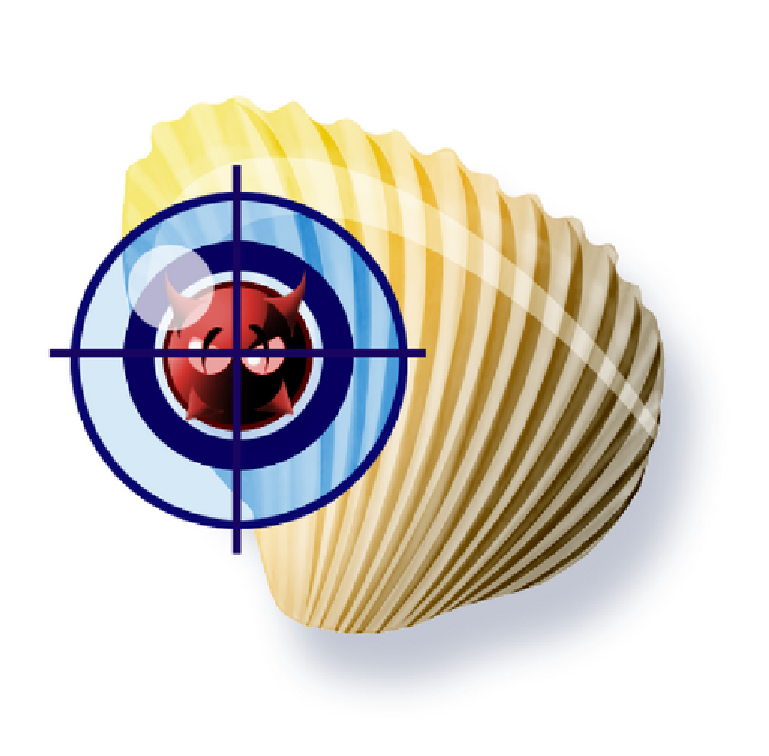
\includegraphics[width=353pt]{clam}
\vspace{3cm}
\begin{flushright}
  \rule[-1ex]{8cm}{3pt}\\
  \huge ClamAV Bytecode Compiler\\
        \huge \emph{User Manual}\\
\end{flushright}
\newpage
\setcounter{page}{1}
\pagestyle{fancy}
\tableofcontents
\vspace{1.0cm}
\noindent
\begin{boxedminipage}[b]{\textwidth}
    ClamAV Bytecode Compiler - Internals Manual,\\
    \copyright \  2009 Sourcefire, Inc.\\
    Authors: T\"{o}r\"{o}k Edvin\\
    This document is distributed under the terms of the GNU General
    Public License v2.\\

    Clam AntiVirus is free software; you can redistribute it and/or modify
    it under the terms of the GNU General Public License as published by
    the Free Software Foundation; version 2 of the License.\\

    This program is distributed in the hope that it will be useful,
    but WITHOUT ANY WARRANTY; without even the implied warranty of
    MERCHANTABILITY or FITNESS FOR A PARTICULAR PURPOSE.  See the
    GNU General Public License for more details.\\

    You should have received a copy of the GNU General Public License
    along with this program; if not, write to the Free Software
    Foundation, Inc., 51 Franklin Street, Fifth Floor, Boston,
    MA 02110-1301, USA.
\end{boxedminipage}

\vspace{0.3cm}
\noindent
\begin{boxedminipage}[b]{\textwidth}
    ClamAV and Clam AntiVirus are trademarks of Sourcefire, Inc.
\end{boxedminipage}
\setlength{\parindent}{18pt}
\mainmatter
\chapter{Overview}

This manual describes internals details about the bytecode API, compiler, and
libclamav bytecode interpreter/JIT.
This manual is only of interest to ClamAV developers, see the
"ClamAV Bytecode Compiler User Manual" on how to write bytecode signatures.

\chapter{Installation}
\section{Requirements}
The ClamAV Bytecode Compiler uses the LLVM compiler framework, thus requires an Operating System
where building LLVM is supported:
\begin{itemize}
 \item FreeBSD/x86
 \item Linux/\{x86,x86\_64,ppc\}
 \item Mac OS X/\{x86,ppc\}
 \item Solaris/sparcv9
 \item Windows/x86 using mingw32 or Visual Studio
\end{itemize}

The following packages are required to compile the ClamAV Bytecode Compiler:
\begin{itemize}
 \item GCC C and C++ compilers (minimum 4.1.3, recommended: 4.3.4 or newer)
\footnote{Note that several versions of GCC have bugs when compiling LLVM, see \url{http://llvm.org/docs/GettingStarted.html\#brokengcc} for a full list.
Also LLVM requires support for atomic builtins for multithreaded mode, which gcc 3.4.x doesn't have}.
 \item Perl (version 5.6.0+)
 \item GNU make (version 3.79+, recommended 3.81)
\end{itemize}

The following packages are optional, but highly recommended:
\begin{itemize}
 \item Python (version 2.5.4+?) - for running the tests
\end{itemize}

\section{Obtaining the ClamAV Bytecode Compiler}
You can obtain the source code in one of the following ways \footnote{For now the use the internal clamtools repository:\\
git clone username@git.clam.sourcefire.com:/var/lib/git/clamtools.git}
\begin{itemize}
 \item Check out the source code using git native protocol:

 \verb+git clone git://git.clamav.net/git/clamav-bytecode-compiler+
 \item Check out the source code using HTTP:

 \verb+git clone http://git.clamav.net/git/clamav-bytecode-compiler.git+
\end{itemize}

You can keep the source code updated using:

\verb+git pull+

\section{Building}
\subsection{Disk space}
A minimalistic release build requires ~100M of disk space.

Testing the compiler requires a full build, ~320M of disk space.
A debug build requires significantly more disk space (1.4G for a minimalistic
debug build).

Note that this only needed during the build process, once installed only ~12M
is needed.

\subsection{Create build directory}
Building requires a separate object directory, building in the source directory is not supported.
Create a build directory:

\verb+$ cd clamav-bytecode-compiler && mkdir obj+

Run configure (you can use any prefix you want, this example uses \verb+/usr/local/clamav+):
\begin{verbatim}
$ cd obj && ../llvm/configure --enable-optimized \
 --enable-targets=host-only --disable-bindings \
--prefix=/usr/local/clamav
\end{verbatim}

Run the build under ulimit \footnote{compiling some files can be very memory intensive, especially with older compilers}:
\begin{verbatim}
$ (ulimit -t 3600 -v 512000 && make clambc-only -j4)
\end{verbatim}

\section{Testing}
\begin{verbatim}
$ (ulimit -t 3600 v 512000 && make -j4)
$ make check-all
\end{verbatim}

If make check reports errors, check that your compiler is NOT on this list:
\url{http://llvm.org/docs/GettingStarted.html#brokengcc}.

If it is, then your compiler is buggy, and you need to do one of the following: upgrade your compiler
to a non-buggy version, upgrade the OS to one that has a non-buggy compiler, compile with \verb|export OPTMIZE_OPTION=-O2|, or
\verb|export OPTIMIZE_OPTION=-O1|, or \verb|export OPTIMIZE_OPTION=\-O1|.

If not you probably found a bug, report it at \url{http://bugs.clamav.net}

\section{Installing}
Install it:
\begin{verbatim}
$ make install-clambc -j8
\end{verbatim}

\subsection{Structure of installed files}
\begin{enumerate}
\item The ClamAV Bytecode compiler driver:
\verb+$PREFIX/bin/clambc-compiler+
\item  ClamAV bytecode header files:
\begin{verbatim}
$PREFIX/lib/clang/1.1/include:
bcfeatures.h
bytecode_{api_decl.c,api,disasm,execs,features}.h
bytecode.h
bytecode_{local,pe,types}.h
\end{verbatim}
\item clang compiler (with ClamAV bytecode backend) compiler include files:
\begin{verbatim}
$PREFIX/lib/clang/1.1/include:
emmintrin.h
float.h
iso646.h
limits.h
{,p,t,x}mmintrin.h
mm_malloc.h
std{arg,bool,def,int}.h
tgmath.h
\end{verbatim}
\item User manual
\begin{verbatim}
$PREFIX/docs/clamav/clambc-user.pdf
\end{verbatim}
\end{enumerate}


\chapter{Tutorial}
\section{Short introduction to the bytecode language}
\subsection{Types, variables and constants}
\subsection{Arrays and pointers}
\subsection{Arithmetics}
\subsection{Functions}
\subsection{Control flow}
\subsection{Common functions}

\section[Writing logical signatures]{Writing logical signature bytecodes}
\footnote{See \prettyref{sec:lsigs} for more details about logical signatures in
bytecode.}
Logical signatures can be used as triggers for executing bytecode. 
However, instead of describing a logical signature as a \verb+.ldb+ pattern, you use (simple) C code which is later
translated to a \verb+.ldb+-style logical signature by the ClamAV Bytecode Compiler.

A bytecode triggered by a logical signature is much more powerful than a logical signature itself:
you can write complex algorithmic detections, and use the logical signature as a \emph{filter} (to speed up matching).
Thus another name for ``logical signature bytecodes'' is ``algorithmic detection bytecodes''.
The detection you write in bytecode has read-only access to the file being scanned and its metadata
(PE sections, EP, etc.).

\subsection{Structure of a bytecode for algorithmic detection}
Algorithmic detection bytecodes are triggered when a logical signature matches.
They can execute an algorithm that determines whether the file is infected and
with which virus.

A bytecode can be either algorithmic or an unpacker (or other hook), but not both.

It consists of:
\begin{itemize}
 \item Definition of virusnames used in the bytecode
 \item Pattern definitions (for logical subexpressions)
 \item The logical signature as C function: \verb+bool logical_trigger(void)+
 \item The \verb+int entrypoint(void)+ function which gets executed when the logical signature matches
 \item (Optional) Other functions and global constants used in \verb+entrypoint+
\end{itemize}

The syntax for defining logical signatures, and an example is described in \prettyref{sec:lsigstut}.

The function \verb+entrypoint+ must report the detected virus by calling \verb+foundVirus+ and returning \verb+0+.
It is recommended that you always return \verb+0+, otherwise a warning is shown and the file is considered clean.
If \verb+foundVirus+ is not called, then ClamAV also assumes the file is clean.

\subsection{Virusnames}
Each logical signature bytecode must have a virusname prefix, and one or more virusnames.
The virusname prefix is used by the SI to ensure unique virusnames (a unique number is appended for duplicate prefixes).

\begin{program}
\begin{lstlisting}
/* Prefix, used for duplicate detection and fixing */
VIRUSNAME_PREFIX("Trojan.Foo")
/* You are only allowed to set these virusnames as found */
VIRUSNAMES("A", "B")
/* File type */
TARGET(2)
\end{lstlisting}
\caption{Declaring virusnames}
\label{prg:virname}
\end{program}

In \prettyref{prg:virname} 3 predefied macros are used:
\begin{itemize}
 \item \verb+VIRUSNAME_PREFIX+ which must have exactly one string argument
 \item \verb+VIRUSNAMES+ which must have one or more string arguments
 \item \verb+TARGET+ which must have exactly one integer argument
\end{itemize}

In this example, the bytecode could generate one of these virusnames:
\verb+Trojan.Foo.A+, or \verb+Trojan.Foo.B+, by calling
\verb+foundVirus("A")+ or \verb+foundVirus("B")+ respectively (notice that the prefix is not part of these calls).

\subsection{Patterns}
Logical signatures use \verb+.ndb+ style patterns, an example on how to define these
is shown in \prettyref{prg:patterns}.
\begin{program}
\begin{lstlisting}
SIGNATURES_DECL_BEGIN
DECLARE_SIGNATURE(magic)
DECLARE_SIGNATURE(check)
DECLARE_SIGNATURE(zero)
SIGNATURES_DECL_END

SIGNATURES_DEF_BEGIN
DEFINE_SIGNATURE(magic, "EP+0:aabb")
DEFINE_SIGNATURE(check, "f00d")
DEFINE_SIGNATURE(zero, "ffff")
SIGNATURES_END
\end{lstlisting}
\caption{Declaring patterns}
\label{prg:patterns}
\end{program}

Each pattern has a name (like a variable), and a string that is the hex pattern itself.
The declarations are delimited by the macros \verb+SIGNATURES_DECL_BEGIN+, and \verb+SIGNATURES_DECL_END+.
The definitions are delimited by the macros \verb+SIGNATURES_DEF_BEGIN+, and \verb+SIGNATURES_END+.
Declarations must always come before definitions, and you can have only one
declaration and declaration section!
(think of declaration like variable
declarations, and definitions as variable assignments, since that what they are under the hood).
The order in which you declare the signatures is the order in which they appear in the generated
logical signature.

You can use any name for the patterns that is a valid record field name in C, 
and doesn't conflict with anything else declared.

After using the above macros, the global variable \verb+Signatures+ will have two new fields:
\verb+magic+, and \verb+zero+.
These can be used as arguments to the functions \verb+count_match()+, and \verb+matches()+
anywhere in the program as shown in \prettyref{prg:counting}:
\begin{itemize}
 \item \verb+matches(Signatures.match)+ will return true when the \verb+match+ signature matches (at least once)
 \item \verb+count_match(Signatures.zero)+ will return the number of times the \verb+zero+ signature matched
 \item \verb+count_match(Signatures.check)+ will return the number of times the \verb+check+ signature matched
\end{itemize}

The condition in the \verb+if+ can be interpreted as: if the \verb+match+ signature has matched at least once,
and the number of times the \verb+zero+ signature matched is higher than the number of times the \verb+check+ signature matched,
then we have found a virus \verb+A+, otherwise the file is clean.

\begin{program}
\begin{lstlisting}
int entrypoint(void)
{
  if (matches(Signatures.match) && count_match(Signatures.zero) > count_match(Signatures.check))
    foundVirus("A");
  return 0;
}
\end{lstlisting}
\caption{Using patterns}
\label{prg:counting}
\end{program}

\subsection{Single subsignature}
\label{sec:lsigstut}
The simplest logical signature is like a \verb+.ndb+ signature: a virus name, signature target, 0 as logical expression
\footnote{meaning that subexpression 0 must match}, and a \verb+ndb+-style pattern.

The code for this is shown in \prettyref{prg:singlesig}
\begin{program}
\lstinputlisting{../../examples/in/lsig_simple.o1.c}
\caption{Single subsignature example}
\label{prg:singlesig}
\end{program}

The logical signature (created by the compiler) looks like this:
\verb+Trojan.Foo.{A};Target:2;0;aabb+

Of course you should use a \verb+.ldb+ signature in this case when all the processing in \verb+entrypoint+
is only setting a virusname and returning.
However, you can do more complex checks in \verb+entrypoint+, once the bytecode was triggered by the \verb+logical_trigger+

In the example in \prettyref{prg:singlesig} the pattern was used without an anchor; such a pattern matches at any offset.
You can use offsets though, the same way as in \verb+.ndb+ signatures, see \prettyref{prg:multisig} for an example.

\subsection{Multiple subsignatures}
An example for this is shown in \prettyref{prg:multisig}.
Here you see the following new features used:
\footnote{In case of a duplicate virusname the
prefix is appended a unique number by the SI}
\begin{itemize}
 \item Multiple virusnames returned from a single bytecode (with common prefix) 
 \item Multiple subsignatures, each with a name of your choice
 \item A pattern with an anchor (\verb|EP+0:aabb|)
 \item More subsignatures defined than used in the logical expression
\end{itemize}

The logical signature looks like this:

\noindent
{\footnotesize
\verb/Trojan.Foo.{A,B};Target:2;(((0|1|2)=42,2)|(3=10));EP+0:aabb;ffff;aaccee;f00d;dead/
}

Notice how the subsignature that is not used in the logical expression (number 4, \verb+dead+)
is used in \verb+entrypoint+ to decide the virus name.
This works because ClamAV does collect the match counts for all subsignatures (regardless if they are used or not in
a signature). The \verb+count_match(Signatures.check2)+ call is thus a simple memory read of the count already determined by ClamAV.

Also notice that comments can be used freely: they are ignored by the compiler. You can use either C-style multiline comments
(start comment with \verb+/*+, end with \verb+*/+), or C++-style single-line comments
(start comment with \verb+//+, automatically ended by newline).

\begin{program}
\lstinputlisting{../../examples/in/lsig.o1.c}
\caption{Multiple subsignatures}
\label{prg:multisig}
\end{program}

\subsection{W32.Polipos.A detector rewritten as bytecode}
\subsection{Virut detector in bytecode}
\section{Writing unpackers}
\label{sec:unpacker}
\subsection{Structure of a bytecode for unpacking (and other hooks)}
When writing an unpacker, the bytecode should consist of:
\begin{itemize}
 \item Define which hook you use (for example \verb+PE_UNPACKER_DECLARE+ for a PE hook)
 \item An \verb+int entrypoint(void)+ function that reads the current file and unpacks it to a new file
 \item Return 0 from \verb+entrypoint+ if you want the unpacked file to be scanned %TODO: how do we avoid infinite recursion
% here, if the bytecode is invoked again, and unpacks something again? Or mutual recursion...
%TODO: I don't call magicscandesc yet, until a solution is found here
 \item (Optional) Other functions and global constants used by \verb+entrypoint+
\end{itemize}

\subsection{Detecting clam.exe via bytecode}
Example provided by aCaB:
\subsection{Detecting clam.exe via bytecode (disasm)}
Example provided by aCaB:

\label{prg:matchclamexedisasm}
\subsection{A simple unpacker}
\subsection{Matching PDF javascript}

\subsection{YC unpacker rewritten as bytecode}

\chapter{Usage}
\section{Invoking the compiler}
Compiling is similar to gcc \footnote{Note that the ClamAV bytecode compiler will refuse to compile code it considers insecure}:
\begin{verbatim}
$ /usr/local/clamav/bin/clambc-compiler foo.c -o foo.cbc -O2
\end{verbatim}

This will compile the file \verb+foo.c+ into a file called \verb+foo.cbc+,
that can be loaded by ClamAV, and packed inside a \verb+.cvd+ file.

The compiler by default has all warnings turned on.

Supported optimization levels: \verb+-O0, -O1, -O2, -O3+. \footnote{Currently -O0 doesn't work}
It is recommended that you always compile with at least \verb+-O1+.

Warning options: \verb+-Werror+ (transforms all warnings into errors).

Preprocessor flags:
\begin{description}
 \item[-I <directory>] Searches in the given directory when it encounters a \verb+#include "headerfile"+ directive in the source code, in addition
to the system defined header search directories.
 \item[-D <MACRONAME>=<VALUE>] Predefine given \verb+<MACRONAME>+ to be equal to \verb+<VALUE>+.
 \item[-U <MACRONAME>] Undefine a predefined macro
\end{description}

The compiler also supports some other commandline options (see \verb+clambc-compiler --help+ for a full list),
however some of them have no effect when using the ClamAV bytecode backend (such as the X86 backend options).
You shouldn't need to use any flags not documented above.

\subsection{Compiling C++ files}
Filenames with a \verb+.cpp+ extension are compiled as C++ files, however \verb|clang++| is not yet
ready for production use, so this is EXPERIMENTAL currently.
For now write bytecodes in C.

\section{Running compiled bytecode}
After compiling a C source file to bytecode, you can load it in ClamAV:
\subsection{ClamBC}
ClamBC is a tool you can use to test whether the bytecode loads, compiles, and can execute its entrypoint successfully.
Usage:
\begin{verbatim}
 clambc <file> [function] [param1 ...]
\end{verbatim}

For example loading a simple bytecode with 2 functions is done like this:
\begin{verbatim}
$ clambc foo.cbc
LibClamAV debug: searching for unrar, user-searchpath: /usr/local/lib
LibClamAV debug: unrar support loaded from libclamunrar_iface.so.6.0.4 libclamunrar_iface_so_6_0
LibClamAV debug: bytecode: Parsed 0 APIcalls, maxapi 0
LibClamAV debug: Parsed 1 BBs, 2 instructions
LibClamAV debug: Parsed 1 BBs, 2 instructions
LibClamAV debug: Parsed 2 functions
Bytecode loaded
Running bytecode function :0
Bytecode run finished
Bytecode returned: 0x8
Exiting
\end{verbatim}

\subsection{clamscan, clamd}
You can tell clamscan to load the bytecode as a database directly:
\begin{verbatim}
$ clamscan -dfoo.cbc
\end{verbatim}
Or you can instruct it to load all databases from a directory, then clamscan will
load all supported formats, including files with bytecode, which have the \verb+.cbc+ extension.
\begin{verbatim}
$ clamscan -ddirectory
\end{verbatim}

% TODO: we should describe or point to the security levels here when they get implemented
You can also put the bytecode files into the default database directory of ClamAV
(usually \verb+/usr/local/share/clamav+) to have it loaded automatically from there.
Of course, the bytecode can be stored inside CVD files, too.

\section{Debugging bytecode}
\subsection{``printf'' style debugging}
You can use \verb+debug_print_str+ and \verb+debug_print_int+ API %TODO: link to API section
calls to print debug messages during the execution of the bytecode.

\subsection{Single-stepping}
%TODO: some glue code missing here: LLVM supports generation of dwarf debug info (including variable and line number info),
%however variable debug info is lost during the most simple transform (mem2reg), and is undergoing a major redesign now,
%and line number debug info is only emited when compiling statically.
%Although line number debug info IS available in the JIT (assuming the loaded bytecode has it, by default it doesn't),
%it currently doesn't emit dwarf debug info at all when JITing.
% So what works is call frame info, i.e. backtraces, and function names in backtraces
If you have GDB 7.0 (or newer) you can single-step \footnote{not yet implemented in libclamav} \footnote{assuming you have JIT support}
during the execution of the bytecode.
\begin{itemize}
 \item Run clambc or clamscan under gdb:
\begin{verbatim}
$ ./libtool --mode=execute gdb clamscan/clamscan
...
(gdb) b cli_vm_execute_jit
Are you sure ....? y
(gdb) run -dfoo.cbc
...
Breakpoint ....

(gdb) step
(gdb) next
\end{verbatim}

You can single-step through the execution of the bytecode, however you can't (yet) print values of individual variables,
you'll need to add debug statements in the bytecode to print interesting values.

\end{itemize}



\chapter{ClamAV bytecode language}
The bytecode that ClamAV loads is a simplified form of the LLVM Intermediate Representation, and as such it is language-independent.

However currently the only supported language from which such bytecode can be generated is a simplified form of C
\footnote{In the future more languages could be supported, see the Internals Manual on language frontends}

The language supported by the ClamAV bytecode compiler is a restricted set of C99 with some GNU extensions.

\section{Differences from C99 and GNU C}
\label{sec:diffc}
These restrictions are enforced at compile time:
\begin{itemize}
 \item No standard include files. \footnote{For portability reasons: preprocessed C code is not portable}
 \item The ClamAV API header files are preincluded.
 \item No external function calls, except to the ClamAV API \footnote{For safety reasons we can't allow the bytecode to call arbitrary system functions}
 \item No inline assembly \footnote{This is both for safety and portability reasons}
 \item Globals can only be readonly constants \footnote{For thread safety reasons}
 \item \verb+inline+ is C99 inline (equivalent to GNU C89 extern inline), thus it cannot be used outside of the definition of the ClamAV API,
you should use \verb+static inline+
 \item \verb+sizeof(int) == 4+ always
 \item \verb+sizeof(long) == sizeof(long long) == 8+ always
 \item \verb+ptr_diff_t = int+, \verb+intptr_t = int+, \verb+intmax_t = long+, \verb+uintmax_t = unsigned long+ 
\footnote{Note that a pointer's sizeof is runtime-platform dependent, although at compile time sizeof(void*) == 4, at runtime it can be something else.
Thus you should avoid using sizeof(pointer)}
 \item No pointer to integer casts and integer to pointer casts (pointer arithmetic is allowed though)
 \item No \verb+__thread+ support
 \item Size of memory region associated with each pointer must be known in each function, thus if you pass a pointer to a function,
you must also pass its allocated size as a parameter.
 \item Endianness must be handled via the \verb+__is_bigendian()+ API function call, or via the \verb+cli_{read,write}int{16,32}+ wrappers,
and not by casting pointers
 \item Predefines \verb+__CLAMBC__+
 \item All integer types have fixed width
 \item \verb+main+ or \verb+entrypoint+ must have the following prototype: \verb+int main(void)+, the prototype
\verb+int main(int argc, char *argv[])+ is not accepted %TODO: really reject this, for now its compiled but clamav won't find main when loading
%TODO: The ClamBC backend should default to bigendian, so that such endianness bugs are caught soon, i.e. they will be immediately buggy when executing on x86,
% unless the endian macros are used
\end{itemize}

They are meant to ensure the following:
\begin{itemize}
 \item Thread safe execution of multiple different bytecodes, and multiple instances of the same bytecode
 \item Portability to multiple CPU architectures and OSes: the bytecode must execute on both the libclamav/LLVM JIT where that is supported (x86, x86\_64, ppc, arm?),
and on the libclamav interpreter where that is not supported.
 \item No external runtime dependency: libclamav should have everything needed to run the bytecode, thus no external calls are allowed, not even to libc!
 \item Same behaviour on all platforms: fixed size integers. 
\end{itemize}

These restrictions are checked at runtime (checks are inserted at compile time):
\begin{itemize}
 \item Accessing an out-of-bounds pointer will result in a call to \verb+abort()+
 \item Calling \verb+abort()+ interrupts the execution of the bytecode in a thread safe manner, and doesn't halt ClamAV
\footnote{in fact it calls a ClamAV API function, and not the libc abort function.}.
\end{itemize}

The ClamAV API header has further restriction, see the Internals manual.

Although the bytecode undergoes a series of automated tests (see Publishing chapter in Internals manual), the above restrictions don't guarantee
that the resulting bytecode will execute correctly!
You must still test the code yourself, these restrictions only avoid the most common errors.
Although the compiler and verifier aims to accept only code that won't crash ClamAV, no code is 100\% perfect, and a bug in the verifier
could allow unsafe code be executed by ClamAV.

\section{Limitations}
The bytecode format has the following limitations:
\begin{itemize}
 \item At most 64k bytecode kinds (hooks)
 \item At most 64k types (including pointers, and all nested types)
 \item At most 16 parameters to functions, no vararg functions
 \item At most 64-bit integers
 \item No vector types or vector operations
 \item No opaque types
 \item No floating point
 \item Global variable initializer must be compile-time computable
 \item At most 32k global variables (and at most 32k API globals)
 \item Pointer indexing at most 15 levels deep (can be worked around if needed by using temporaries)
 \item No struct return or byval parameters
 \item At most 32k instructions in a single function
 \item No Variable Length Arrays
\end{itemize}



\section{Logical signatures}
\label{sec:lsigs}
Logical signatures can be used as triggers for executing a bytecode. 
Instead of describing a logical signatures as a \verb+.ldb+ pattern, you use C code which is then
translated to a \verb+.ldb+-style logical signature.

Logical signatures in ClamAV support the following operations:
\begin{itemize}
 \item Sum the count of logical subsignatures that matched inside a subexpression
 \item Sum the number of different subsignatures that matched inside a subexpression
 \item Compare the above counts using the $>,=,<$ relation operators
 \item Perform logical $\&\&, ||$ operations on above boolean values
 \item Nest subexpressions
 \item Maximum 64 subexpressions
\end{itemize}

Out of the above operations the ClamAV Bytecode Compiler doesn't support computing sums of nested subexpressions,
(it does support nesting though).

The C code that can be converted into a logical signature must obey these restrictions:
\begin{itemize}
 \item a function named \verb+logical_trigger+ with the following prototype:
\verb+bool logical_trigger(void)+
 \item no function calls, except for \verb+count_match+ and \verb+matches+
 \item no global variable access (except as done by the above 2 functions internally)
 \item return true when signature should trigger, false otherwise
 \item use only integer compare instructions, branches, integer \emph{add}, logical \emph{and}, logical \emph{or},
logical \emph{xor}, zero extension, store/load from local variables
 \item the final boolean expression must be convertible to disjunctive normal form without negation
 \item the final logical expression must not have more than 64 subexpressions
 \item it can have early returns (all true returns are unified using $||$)
 \item you can freely use comments, they are ignored
 \item the final boolean expression cannot be a \verb+true+ or \verb+false+ constant
\end{itemize}

The compiler does the following transformations (not necessarily in this order):
\begin{itemize}
 \item convert shortcircuit boolean operations into non-shortcircuit ones (since all operands are boolean expressions or local variables,
it is safe to execute these unconditionally)
 \item propagate constants
 \item simplify control flow graph
 \item (sparse) conditional constant propagation
 \item dead store elimination
 \item dead code elimination
 \item instruction combining (arithmetic simplifications)
 \item jump threading
\end{itemize}

If after this transformation the program meets the requirements outlined above, then it is converted to a logical signature.
The resulting logical signature is simplified using basic properties of boolean operations, such as
associativity, distributivity, De Morgan's law.

The final logical signature is not unique (there might be another logical signature with identical behavior), however the boolean part is in a canonical form:
it is in disjunctive normal form, with operands sorted in ascending order.

For best results the C code should consist of:
\begin{itemize}
 \item local variables declaring the sums you want to use
 \item a series of \verb+if+ branches that \verb+return true+, where the \verb+if+'s condition is a single comparison or a logical \emph{and} of comparisons
 \item a final \verb+return false+
\end{itemize}

You can use $||$ in the \verb+if+ condition too, but be careful that after expanding to disjunctive normal form, the number of subexpressions doesn't exceed 64.

Note that you do not have to use all the subsignatures you declared in \verb+logical_trigger+, you can
do more complicated checks (that wouldn't obey the above restrictions) in the bytecode itself at runtime.
The \verb+logical_trigger+ function is fully compiled into a logical signature, it won't be a runtime executed function (hence the restrictions).

\section{Headers and runtime environment}
When compiling a bytecode program, \verb+bytecode.h+ is automatically included, so you don't need to explicitly include it.
These headers (and the compiler itself) predefine certain macros, see \prettyref{apdx:predefined} for a full list.
In addition the following types are defined:
\begin{lstlisting}
typedef unsigned char uint8_t;
typedef char int8_t;
typedef unsigned short uint16_t;
typedef short int16_t;
typedef unsigned int uint32_t;
typedef int int32_t;
typedef unsigned long uint64_t;
typedef long int64_t;
typedef unsigned int size_t;
typedef int off_t;
typedef struct signature { unsigned id } __Signature;
\end{lstlisting}
As described in \prettyref{sec:diffc} the width of integer types are fixed, the above typedefs show that.

A bytecode's entrypoint is the function \verb+entrypoint+ and it's required by ClamAV to load the bytecode.

Bytecode that is triggered by a logical signature must have a list of virusnames and patterns defined.
Bytecodes triggered via hooks can optionally have them, but for example a PE unpacker doesn't need virus
names as it only processes the data.

\chapter{Bytecode security \& portability}
%TODO: fill in

\chapter{Reporting bugs}
\chapter{Bytecode API}
\setlength{\parindent}{0pt}
\section{API groups}
\subsection{Bytecode configuration}
\label{config}
\hypertarget{config}{}
\input{../doxygen/latex/config}
\subsection{Data structure handling functions}
\label{adt}
\hypertarget{adt}{}
\input{../doxygen/latex/adt}
\subsection{Disassemble APIs}
\label{disasm}
\hypertarget{disasm}{}
\input{../doxygen/latex/disasm}
\subsection{Engine queries}
\label{engineq}
\hypertarget{engineq}{}
\input{../doxygen/latex/engineq}
\subsection{Environment detection functions}
\label{envdet}
\hypertarget{envdet}{}
\input{../doxygen/latex/envdet}
\subsection{File operations}
\label{fileops}
\hypertarget{fileops}{}
\input{../doxygen/latex/fileops}
\subsection{Global variables}
\label{globals}
\hypertarget{globals}{}
\input{../doxygen/latex/globals}
\subsection{Icon matcher APIs}
\label{icon}
\hypertarget{icon}{}
\input{../doxygen/latex/icon}
\subsection{JS normalize API}
\label{js}
\hypertarget{js}{}
\input{../doxygen/latex/js}
\subsection{Math functions}
\label{math}
\hypertarget{math}{}
\input{../doxygen/latex/math}
\subsection{PDF handling functions}
\label{pdfg}
\hypertarget{pdfg}{}
\input{../doxygen/latex/pdfg}
\subsection{PE functions}
\label{pe}
\hypertarget{pe}{}
\input{../doxygen/latex/pe}
\subsection{Scan control functions}
\label{scanc}
\hypertarget{scanc}{}
\input{../doxygen/latex/scanc}
\subsection{String operations}
\label{stringops}
\hypertarget{stringops}{}
\input{../doxygen/latex/stringops}
\section{Structure types}
\hypertarget{structcli__exe__info}{
\subsection{cli\_\-exe\_\-info Struct Reference}
\label{structcli__exe__info}\index{cli\_\-exe\_\-info@{cli\_\-exe\_\-info}}
}
\subsubsection*{Data Fields}
\begin{DoxyCompactItemize}
\item 
struct \hyperlink{structcli__exe__section}{cli\_\-exe\_\-section} $\ast$ \hyperlink{structcli__exe__info_a1c449c2a02971006b72d8ab755684716}{section}
\item 
uint32\_\-t \hyperlink{structcli__exe__info_a894bdfa2d603d8343f8ef01dda6fcd23}{offset}
\item 
uint32\_\-t \hyperlink{structcli__exe__info_afaed4671662028c061ab84eefcce0546}{ep}
\item 
uint16\_\-t \hyperlink{structcli__exe__info_aa4af5e526457df524fc9a4ba46803a70}{nsections}
\item 
uint32\_\-t \hyperlink{structcli__exe__info_ac0f1b36bb8a1eeb981958dc4643f67dd}{res\_\-addr}
\item 
uint32\_\-t \hyperlink{structcli__exe__info_af2492dd421362ffced98eb583964b310}{hdr\_\-size}
\end{DoxyCompactItemize}


\subsubsection{Detailed Description}
Executable file information \begin{Desc}
\item[\hyperlink{pe__pe000004}{PE}]\end{Desc}


\subsubsection{Field Documentation}
\hypertarget{structcli__exe__info_afaed4671662028c061ab84eefcce0546}{
\index{cli\_\-exe\_\-info@{cli\_\-exe\_\-info}!ep@{ep}}
\index{ep@{ep}!cli_exe_info@{cli\_\-exe\_\-info}}
\paragraph[{ep}]{\setlength{\rightskip}{0pt plus 5cm}uint32\_\-t {\bf ep}}}
\label{structcli__exe__info_afaed4671662028c061ab84eefcce0546}
Entrypoint of executable \hypertarget{structcli__exe__info_af2492dd421362ffced98eb583964b310}{
\index{cli\_\-exe\_\-info@{cli\_\-exe\_\-info}!hdr\_\-size@{hdr\_\-size}}
\index{hdr\_\-size@{hdr\_\-size}!cli_exe_info@{cli\_\-exe\_\-info}}
\paragraph[{hdr\_\-size}]{\setlength{\rightskip}{0pt plus 5cm}uint32\_\-t {\bf hdr\_\-size}}}
\label{structcli__exe__info_af2492dd421362ffced98eb583964b310}
Address size -\/ PE ONLY \hypertarget{structcli__exe__info_aa4af5e526457df524fc9a4ba46803a70}{
\index{cli\_\-exe\_\-info@{cli\_\-exe\_\-info}!nsections@{nsections}}
\index{nsections@{nsections}!cli_exe_info@{cli\_\-exe\_\-info}}
\paragraph[{nsections}]{\setlength{\rightskip}{0pt plus 5cm}uint16\_\-t {\bf nsections}}}
\label{structcli__exe__info_aa4af5e526457df524fc9a4ba46803a70}
Number of sections \hypertarget{structcli__exe__info_a894bdfa2d603d8343f8ef01dda6fcd23}{
\index{cli\_\-exe\_\-info@{cli\_\-exe\_\-info}!offset@{offset}}
\index{offset@{offset}!cli_exe_info@{cli\_\-exe\_\-info}}
\paragraph[{offset}]{\setlength{\rightskip}{0pt plus 5cm}uint32\_\-t {\bf offset}}}
\label{structcli__exe__info_a894bdfa2d603d8343f8ef01dda6fcd23}
Offset where this executable start in file (nonzero if embedded) \hypertarget{structcli__exe__info_ac0f1b36bb8a1eeb981958dc4643f67dd}{
\index{cli\_\-exe\_\-info@{cli\_\-exe\_\-info}!res\_\-addr@{res\_\-addr}}
\index{res\_\-addr@{res\_\-addr}!cli_exe_info@{cli\_\-exe\_\-info}}
\paragraph[{res\_\-addr}]{\setlength{\rightskip}{0pt plus 5cm}uint32\_\-t {\bf res\_\-addr}}}
\label{structcli__exe__info_ac0f1b36bb8a1eeb981958dc4643f67dd}
Resrources RVA -\/ PE ONLY \hypertarget{structcli__exe__info_a1c449c2a02971006b72d8ab755684716}{
\index{cli\_\-exe\_\-info@{cli\_\-exe\_\-info}!section@{section}}
\index{section@{section}!cli_exe_info@{cli\_\-exe\_\-info}}
\paragraph[{section}]{\setlength{\rightskip}{0pt plus 5cm}struct {\bf cli\_\-exe\_\-section}$\ast$ {\bf section}}}
\label{structcli__exe__info_a1c449c2a02971006b72d8ab755684716}
Information about all the sections of this file. This array has {\ttfamily nsection} elements 
\hypertarget{structcli__exe__section}{\subsection{cli\-\_\-exe\-\_\-section Struct Reference}
\label{structcli__exe__section}\index{cli\-\_\-exe\-\_\-section@{cli\-\_\-exe\-\_\-section}}
}
\subsubsection*{Data Fields}
\begin{DoxyCompactItemize}
\item 
uint32\-\_\-t \hyperlink{structcli__exe__section_a428af6b898632e49e1a78a6b75c35597}{rva}
\item 
uint32\-\_\-t \hyperlink{structcli__exe__section_a4e9a2c96ba84fd9dedbed61c9865cbc7}{vsz}
\item 
uint32\-\_\-t \hyperlink{structcli__exe__section_a0a595268561edc58e347ca8387000bc6}{raw}
\item 
uint32\-\_\-t \hyperlink{structcli__exe__section_a9d1a35dea930f9ddac78908ca3dce76b}{rsz}
\item 
uint32\-\_\-t \hyperlink{structcli__exe__section_a0737a11eee3c5a5d691fade6df9f5094}{chr}
\item 
uint32\-\_\-t \hyperlink{structcli__exe__section_a932862bb5ce030d0e6f007068e7817d6}{urva}
\item 
uint32\-\_\-t \hyperlink{structcli__exe__section_a4241ef43b0b01fea785fe76ba7054a37}{uvsz}
\item 
uint32\-\_\-t \hyperlink{structcli__exe__section_a1c392d2998c0846b21909814e4706a1e}{uraw}
\item 
uint32\-\_\-t \hyperlink{structcli__exe__section_a69f4a0067dad89980f815b5704f5f8da}{ursz}
\end{DoxyCompactItemize}


\subsubsection{Detailed Description}
Section of executable file. 

\subsubsection{Field Documentation}
\hypertarget{structcli__exe__section_a0737a11eee3c5a5d691fade6df9f5094}{\index{cli\-\_\-exe\-\_\-section@{cli\-\_\-exe\-\_\-section}!chr@{chr}}
\index{chr@{chr}!cli_exe_section@{cli\-\_\-exe\-\_\-section}}
\paragraph[{chr}]{\setlength{\rightskip}{0pt plus 5cm}uint32\-\_\-t chr}}\label{structcli__exe__section_a0737a11eee3c5a5d691fade6df9f5094}
Section characteristics \hypertarget{structcli__exe__section_a0a595268561edc58e347ca8387000bc6}{\index{cli\-\_\-exe\-\_\-section@{cli\-\_\-exe\-\_\-section}!raw@{raw}}
\index{raw@{raw}!cli_exe_section@{cli\-\_\-exe\-\_\-section}}
\paragraph[{raw}]{\setlength{\rightskip}{0pt plus 5cm}uint32\-\_\-t raw}}\label{structcli__exe__section_a0a595268561edc58e347ca8387000bc6}
Raw offset (in file) \hypertarget{structcli__exe__section_a9d1a35dea930f9ddac78908ca3dce76b}{\index{cli\-\_\-exe\-\_\-section@{cli\-\_\-exe\-\_\-section}!rsz@{rsz}}
\index{rsz@{rsz}!cli_exe_section@{cli\-\_\-exe\-\_\-section}}
\paragraph[{rsz}]{\setlength{\rightskip}{0pt plus 5cm}uint32\-\_\-t rsz}}\label{structcli__exe__section_a9d1a35dea930f9ddac78908ca3dce76b}
Raw size (in file) \hypertarget{structcli__exe__section_a428af6b898632e49e1a78a6b75c35597}{\index{cli\-\_\-exe\-\_\-section@{cli\-\_\-exe\-\_\-section}!rva@{rva}}
\index{rva@{rva}!cli_exe_section@{cli\-\_\-exe\-\_\-section}}
\paragraph[{rva}]{\setlength{\rightskip}{0pt plus 5cm}uint32\-\_\-t rva}}\label{structcli__exe__section_a428af6b898632e49e1a78a6b75c35597}
Relative Virtual\-Address \hypertarget{structcli__exe__section_a1c392d2998c0846b21909814e4706a1e}{\index{cli\-\_\-exe\-\_\-section@{cli\-\_\-exe\-\_\-section}!uraw@{uraw}}
\index{uraw@{uraw}!cli_exe_section@{cli\-\_\-exe\-\_\-section}}
\paragraph[{uraw}]{\setlength{\rightskip}{0pt plus 5cm}uint32\-\_\-t uraw}}\label{structcli__exe__section_a1c392d2998c0846b21909814e4706a1e}
P\-E -\/ unaligned Pointer\-To\-Raw\-Data \hypertarget{structcli__exe__section_a69f4a0067dad89980f815b5704f5f8da}{\index{cli\-\_\-exe\-\_\-section@{cli\-\_\-exe\-\_\-section}!ursz@{ursz}}
\index{ursz@{ursz}!cli_exe_section@{cli\-\_\-exe\-\_\-section}}
\paragraph[{ursz}]{\setlength{\rightskip}{0pt plus 5cm}uint32\-\_\-t ursz}}\label{structcli__exe__section_a69f4a0067dad89980f815b5704f5f8da}
P\-E -\/ unaligned Size\-Of\-Raw\-Data \hypertarget{structcli__exe__section_a932862bb5ce030d0e6f007068e7817d6}{\index{cli\-\_\-exe\-\_\-section@{cli\-\_\-exe\-\_\-section}!urva@{urva}}
\index{urva@{urva}!cli_exe_section@{cli\-\_\-exe\-\_\-section}}
\paragraph[{urva}]{\setlength{\rightskip}{0pt plus 5cm}uint32\-\_\-t urva}}\label{structcli__exe__section_a932862bb5ce030d0e6f007068e7817d6}
P\-E -\/ unaligned Virtual\-Address \hypertarget{structcli__exe__section_a4241ef43b0b01fea785fe76ba7054a37}{\index{cli\-\_\-exe\-\_\-section@{cli\-\_\-exe\-\_\-section}!uvsz@{uvsz}}
\index{uvsz@{uvsz}!cli_exe_section@{cli\-\_\-exe\-\_\-section}}
\paragraph[{uvsz}]{\setlength{\rightskip}{0pt plus 5cm}uint32\-\_\-t uvsz}}\label{structcli__exe__section_a4241ef43b0b01fea785fe76ba7054a37}
P\-E -\/ unaligned Virtual\-Size \hypertarget{structcli__exe__section_a4e9a2c96ba84fd9dedbed61c9865cbc7}{\index{cli\-\_\-exe\-\_\-section@{cli\-\_\-exe\-\_\-section}!vsz@{vsz}}
\index{vsz@{vsz}!cli_exe_section@{cli\-\_\-exe\-\_\-section}}
\paragraph[{vsz}]{\setlength{\rightskip}{0pt plus 5cm}uint32\-\_\-t vsz}}\label{structcli__exe__section_a4e9a2c96ba84fd9dedbed61c9865cbc7}
Virtual\-Size 
\hypertarget{structcli__pe__hook__data}{
\subsection{cli\_\-pe\_\-hook\_\-data Struct Reference}
\label{structcli__pe__hook__data}\index{cli\_\-pe\_\-hook\_\-data@{cli\_\-pe\_\-hook\_\-data}}
}
\subsubsection*{Data Fields}
\begin{DoxyCompactItemize}
\item 
uint32\_\-t \hyperlink{structcli__pe__hook__data_afaed4671662028c061ab84eefcce0546}{ep}
\item 
uint16\_\-t \hyperlink{structcli__pe__hook__data_aa4af5e526457df524fc9a4ba46803a70}{nsections}
\item 
struct \hyperlink{structpe__image__file__hdr}{pe\_\-image\_\-file\_\-hdr} \hyperlink{structcli__pe__hook__data_a3b996731cad79e0040fc0e4613d20533}{file\_\-hdr}
\item 
struct \hyperlink{structpe__image__optional__hdr32}{pe\_\-image\_\-optional\_\-hdr32} \hyperlink{structcli__pe__hook__data_a5c990dffd52525141865f02731eadf68}{opt32}
\item 
struct \hyperlink{structpe__image__optional__hdr64}{pe\_\-image\_\-optional\_\-hdr64} \hyperlink{structcli__pe__hook__data_ae7195772fb9257482b56b5a65114a479}{opt64}
\item 
struct \hyperlink{structpe__image__data__dir}{pe\_\-image\_\-data\_\-dir} \hyperlink{structcli__pe__hook__data_aacc309d29c73dbd6ac72ee719e331097}{dirs} \mbox{[}16\mbox{]}
\item 
uint32\_\-t \hyperlink{structcli__pe__hook__data_a3d0539adcc53a30b31c2a18bc8b84e00}{e\_\-lfanew}
\item 
uint32\_\-t \hyperlink{structcli__pe__hook__data_af169b0060e4ed3e78fd7ef2588aa7ef6}{overlays}
\item 
int32\_\-t \hyperlink{structcli__pe__hook__data_aed2bc0e93b8e8e291987fc1a2ef801d1}{overlays\_\-sz}
\item 
uint32\_\-t \hyperlink{structcli__pe__hook__data_af2492dd421362ffced98eb583964b310}{hdr\_\-size}
\end{DoxyCompactItemize}


\subsubsection{Detailed Description}
Data for the bytecode PE hook 

\subsubsection{Field Documentation}
\hypertarget{structcli__pe__hook__data_aacc309d29c73dbd6ac72ee719e331097}{
\index{cli\_\-pe\_\-hook\_\-data@{cli\_\-pe\_\-hook\_\-data}!dirs@{dirs}}
\index{dirs@{dirs}!cli_pe_hook_data@{cli\_\-pe\_\-hook\_\-data}}
\paragraph[{dirs}]{\setlength{\rightskip}{0pt plus 5cm}struct {\bf pe\_\-image\_\-data\_\-dir} {\bf dirs}\mbox{[}16\mbox{]}}\hfill}
\label{structcli__pe__hook__data_aacc309d29c73dbd6ac72ee719e331097}
PE data directory header \hypertarget{structcli__pe__hook__data_a3d0539adcc53a30b31c2a18bc8b84e00}{
\index{cli\_\-pe\_\-hook\_\-data@{cli\_\-pe\_\-hook\_\-data}!e\_\-lfanew@{e\_\-lfanew}}
\index{e\_\-lfanew@{e\_\-lfanew}!cli_pe_hook_data@{cli\_\-pe\_\-hook\_\-data}}
\paragraph[{e\_\-lfanew}]{\setlength{\rightskip}{0pt plus 5cm}uint32\_\-t {\bf e\_\-lfanew}}\hfill}
\label{structcli__pe__hook__data_a3d0539adcc53a30b31c2a18bc8b84e00}
address of new exe header \hypertarget{structcli__pe__hook__data_afaed4671662028c061ab84eefcce0546}{
\index{cli\_\-pe\_\-hook\_\-data@{cli\_\-pe\_\-hook\_\-data}!ep@{ep}}
\index{ep@{ep}!cli_pe_hook_data@{cli\_\-pe\_\-hook\_\-data}}
\paragraph[{ep}]{\setlength{\rightskip}{0pt plus 5cm}uint32\_\-t {\bf ep}}\hfill}
\label{structcli__pe__hook__data_afaed4671662028c061ab84eefcce0546}
EntryPoint as file offset \hypertarget{structcli__pe__hook__data_a3b996731cad79e0040fc0e4613d20533}{
\index{cli\_\-pe\_\-hook\_\-data@{cli\_\-pe\_\-hook\_\-data}!file\_\-hdr@{file\_\-hdr}}
\index{file\_\-hdr@{file\_\-hdr}!cli_pe_hook_data@{cli\_\-pe\_\-hook\_\-data}}
\paragraph[{file\_\-hdr}]{\setlength{\rightskip}{0pt plus 5cm}struct {\bf pe\_\-image\_\-file\_\-hdr} {\bf file\_\-hdr}}\hfill}
\label{structcli__pe__hook__data_a3b996731cad79e0040fc0e4613d20533}
Header for this PE file \hypertarget{structcli__pe__hook__data_af2492dd421362ffced98eb583964b310}{
\index{cli\_\-pe\_\-hook\_\-data@{cli\_\-pe\_\-hook\_\-data}!hdr\_\-size@{hdr\_\-size}}
\index{hdr\_\-size@{hdr\_\-size}!cli_pe_hook_data@{cli\_\-pe\_\-hook\_\-data}}
\paragraph[{hdr\_\-size}]{\setlength{\rightskip}{0pt plus 5cm}uint32\_\-t {\bf hdr\_\-size}}\hfill}
\label{structcli__pe__hook__data_af2492dd421362ffced98eb583964b310}
internally needed by rawaddr \hypertarget{structcli__pe__hook__data_aa4af5e526457df524fc9a4ba46803a70}{
\index{cli\_\-pe\_\-hook\_\-data@{cli\_\-pe\_\-hook\_\-data}!nsections@{nsections}}
\index{nsections@{nsections}!cli_pe_hook_data@{cli\_\-pe\_\-hook\_\-data}}
\paragraph[{nsections}]{\setlength{\rightskip}{0pt plus 5cm}uint16\_\-t {\bf nsections}}\hfill}
\label{structcli__pe__hook__data_aa4af5e526457df524fc9a4ba46803a70}
Number of sections \hypertarget{structcli__pe__hook__data_a5c990dffd52525141865f02731eadf68}{
\index{cli\_\-pe\_\-hook\_\-data@{cli\_\-pe\_\-hook\_\-data}!opt32@{opt32}}
\index{opt32@{opt32}!cli_pe_hook_data@{cli\_\-pe\_\-hook\_\-data}}
\paragraph[{opt32}]{\setlength{\rightskip}{0pt plus 5cm}struct {\bf pe\_\-image\_\-optional\_\-hdr32} {\bf opt32}}\hfill}
\label{structcli__pe__hook__data_a5c990dffd52525141865f02731eadf68}
32-\/bit PE optional header \hypertarget{structcli__pe__hook__data_ae7195772fb9257482b56b5a65114a479}{
\index{cli\_\-pe\_\-hook\_\-data@{cli\_\-pe\_\-hook\_\-data}!opt64@{opt64}}
\index{opt64@{opt64}!cli_pe_hook_data@{cli\_\-pe\_\-hook\_\-data}}
\paragraph[{opt64}]{\setlength{\rightskip}{0pt plus 5cm}struct {\bf pe\_\-image\_\-optional\_\-hdr64} {\bf opt64}}\hfill}
\label{structcli__pe__hook__data_ae7195772fb9257482b56b5a65114a479}
64-\/bit PE optional header \hypertarget{structcli__pe__hook__data_af169b0060e4ed3e78fd7ef2588aa7ef6}{
\index{cli\_\-pe\_\-hook\_\-data@{cli\_\-pe\_\-hook\_\-data}!overlays@{overlays}}
\index{overlays@{overlays}!cli_pe_hook_data@{cli\_\-pe\_\-hook\_\-data}}
\paragraph[{overlays}]{\setlength{\rightskip}{0pt plus 5cm}uint32\_\-t {\bf overlays}}\hfill}
\label{structcli__pe__hook__data_af169b0060e4ed3e78fd7ef2588aa7ef6}
number of overlays \hypertarget{structcli__pe__hook__data_aed2bc0e93b8e8e291987fc1a2ef801d1}{
\index{cli\_\-pe\_\-hook\_\-data@{cli\_\-pe\_\-hook\_\-data}!overlays\_\-sz@{overlays\_\-sz}}
\index{overlays\_\-sz@{overlays\_\-sz}!cli_pe_hook_data@{cli\_\-pe\_\-hook\_\-data}}
\paragraph[{overlays\_\-sz}]{\setlength{\rightskip}{0pt plus 5cm}int32\_\-t {\bf overlays\_\-sz}}\hfill}
\label{structcli__pe__hook__data_aed2bc0e93b8e8e291987fc1a2ef801d1}
size of overlays 
\hypertarget{struct_d_i_s__arg}{\subsection{D\-I\-S\-\_\-arg Struct Reference}
\label{struct_d_i_s__arg}\index{D\-I\-S\-\_\-arg@{D\-I\-S\-\_\-arg}}
}
\subsubsection*{Data Fields}
\begin{DoxyCompactItemize}
\item 
enum \hyperlink{bytecode__disasm_8h_a3dcc05be268362b3f772b1675e0a882c}{D\-I\-S\-\_\-\-A\-C\-C\-E\-S\-S} \hyperlink{struct_d_i_s__arg_a5a7d33b48f73c1d560377f10471d8b00}{access\-\_\-type}
\item 
enum \hyperlink{bytecode__disasm_8h_a6a0d419b6b61630b1f76a25ff39df84d}{D\-I\-S\-\_\-\-S\-I\-Z\-E} \hyperlink{struct_d_i_s__arg_abe85ed51a3596cdb3a868a284c3d961f}{access\-\_\-size}
\item 
struct \hyperlink{struct_d_i_s__mem__arg}{D\-I\-S\-\_\-mem\-\_\-arg} \hyperlink{struct_d_i_s__arg_a883edefb091b4875ffd7bb1f1e61dea3}{mem}
\item 
enum \hyperlink{bytecode__disasm_8h_a87af2e927a80478796188d9d8d813d82}{X86\-R\-E\-G\-S} \hyperlink{struct_d_i_s__arg_a426daf7e6de8cea3128731107457d2cf}{reg}
\item 
uint64\-\_\-t \hyperlink{struct_d_i_s__arg_aabf8b24bd58cc13ea953e9add24d4387}{other}
\end{DoxyCompactItemize}


\subsubsection{Detailed Description}
Disassembled operand. 

\subsubsection{Field Documentation}
\hypertarget{struct_d_i_s__arg_abe85ed51a3596cdb3a868a284c3d961f}{\index{D\-I\-S\-\_\-arg@{D\-I\-S\-\_\-arg}!access\-\_\-size@{access\-\_\-size}}
\index{access\-\_\-size@{access\-\_\-size}!DIS_arg@{D\-I\-S\-\_\-arg}}
\paragraph[{access\-\_\-size}]{\setlength{\rightskip}{0pt plus 5cm}enum {\bf D\-I\-S\-\_\-\-S\-I\-Z\-E} access\-\_\-size}}\label{struct_d_i_s__arg_abe85ed51a3596cdb3a868a284c3d961f}
size of access \hypertarget{struct_d_i_s__arg_a5a7d33b48f73c1d560377f10471d8b00}{\index{D\-I\-S\-\_\-arg@{D\-I\-S\-\_\-arg}!access\-\_\-type@{access\-\_\-type}}
\index{access\-\_\-type@{access\-\_\-type}!DIS_arg@{D\-I\-S\-\_\-arg}}
\paragraph[{access\-\_\-type}]{\setlength{\rightskip}{0pt plus 5cm}enum {\bf D\-I\-S\-\_\-\-A\-C\-C\-E\-S\-S} access\-\_\-type}}\label{struct_d_i_s__arg_a5a7d33b48f73c1d560377f10471d8b00}
type of access \hypertarget{struct_d_i_s__arg_a883edefb091b4875ffd7bb1f1e61dea3}{\index{D\-I\-S\-\_\-arg@{D\-I\-S\-\_\-arg}!mem@{mem}}
\index{mem@{mem}!DIS_arg@{D\-I\-S\-\_\-arg}}
\paragraph[{mem}]{\setlength{\rightskip}{0pt plus 5cm}struct {\bf D\-I\-S\-\_\-mem\-\_\-arg} mem}}\label{struct_d_i_s__arg_a883edefb091b4875ffd7bb1f1e61dea3}
memory operand \hypertarget{struct_d_i_s__arg_aabf8b24bd58cc13ea953e9add24d4387}{\index{D\-I\-S\-\_\-arg@{D\-I\-S\-\_\-arg}!other@{other}}
\index{other@{other}!DIS_arg@{D\-I\-S\-\_\-arg}}
\paragraph[{other}]{\setlength{\rightskip}{0pt plus 5cm}uint64\-\_\-t other}}\label{struct_d_i_s__arg_aabf8b24bd58cc13ea953e9add24d4387}
other operand \hypertarget{struct_d_i_s__arg_a426daf7e6de8cea3128731107457d2cf}{\index{D\-I\-S\-\_\-arg@{D\-I\-S\-\_\-arg}!reg@{reg}}
\index{reg@{reg}!DIS_arg@{D\-I\-S\-\_\-arg}}
\paragraph[{reg}]{\setlength{\rightskip}{0pt plus 5cm}enum {\bf X86\-R\-E\-G\-S} reg}}\label{struct_d_i_s__arg_a426daf7e6de8cea3128731107457d2cf}
register operand 
\hypertarget{struct_d_i_s__fixed}{
\subsection{DIS\_\-fixed Struct Reference}
\label{struct_d_i_s__fixed}\index{DIS\_\-fixed@{DIS\_\-fixed}}
}
\subsubsection*{Data Fields}
\begin{DoxyCompactItemize}
\item 
enum \hyperlink{bytecode__disasm_8h_a6bf8b2b4d6261f0e88170a7d0585a5e2}{X86OPS} \hyperlink{struct_d_i_s__fixed_a372354efff5b025dc9324a03625338a2}{x86\_\-opcode}
\item 
enum \hyperlink{bytecode__disasm_8h_a6a0d419b6b61630b1f76a25ff39df84d}{DIS\_\-SIZE} \hyperlink{struct_d_i_s__fixed_a1a17e54c88513da8e5b1175a785c51ae}{operation\_\-size}
\item 
enum \hyperlink{bytecode__disasm_8h_a6a0d419b6b61630b1f76a25ff39df84d}{DIS\_\-SIZE} \hyperlink{struct_d_i_s__fixed_a772bedb1977f1ae07b9f55991f318bd8}{address\_\-size}
\item 
uint8\_\-t \hyperlink{struct_d_i_s__fixed_afbf231e07d12db4d0ebf0bc223679ae5}{segment}
\end{DoxyCompactItemize}


\subsubsection{Detailed Description}
disassembled instruction 

\subsubsection{Field Documentation}
\hypertarget{struct_d_i_s__fixed_a772bedb1977f1ae07b9f55991f318bd8}{
\index{DIS\_\-fixed@{DIS\_\-fixed}!address\_\-size@{address\_\-size}}
\index{address\_\-size@{address\_\-size}!DIS_fixed@{DIS\_\-fixed}}
\paragraph[{address\_\-size}]{\setlength{\rightskip}{0pt plus 5cm}enum {\bf DIS\_\-SIZE} {\bf address\_\-size}}\hfill}
\label{struct_d_i_s__fixed_a772bedb1977f1ae07b9f55991f318bd8}
size of address \hypertarget{struct_d_i_s__fixed_a1a17e54c88513da8e5b1175a785c51ae}{
\index{DIS\_\-fixed@{DIS\_\-fixed}!operation\_\-size@{operation\_\-size}}
\index{operation\_\-size@{operation\_\-size}!DIS_fixed@{DIS\_\-fixed}}
\paragraph[{operation\_\-size}]{\setlength{\rightskip}{0pt plus 5cm}enum {\bf DIS\_\-SIZE} {\bf operation\_\-size}}\hfill}
\label{struct_d_i_s__fixed_a1a17e54c88513da8e5b1175a785c51ae}
size of operation \hypertarget{struct_d_i_s__fixed_afbf231e07d12db4d0ebf0bc223679ae5}{
\index{DIS\_\-fixed@{DIS\_\-fixed}!segment@{segment}}
\index{segment@{segment}!DIS_fixed@{DIS\_\-fixed}}
\paragraph[{segment}]{\setlength{\rightskip}{0pt plus 5cm}uint8\_\-t {\bf segment}}\hfill}
\label{struct_d_i_s__fixed_afbf231e07d12db4d0ebf0bc223679ae5}
segment \hypertarget{struct_d_i_s__fixed_a372354efff5b025dc9324a03625338a2}{
\index{DIS\_\-fixed@{DIS\_\-fixed}!x86\_\-opcode@{x86\_\-opcode}}
\index{x86\_\-opcode@{x86\_\-opcode}!DIS_fixed@{DIS\_\-fixed}}
\paragraph[{x86\_\-opcode}]{\setlength{\rightskip}{0pt plus 5cm}enum {\bf X86OPS} {\bf x86\_\-opcode}}\hfill}
\label{struct_d_i_s__fixed_a372354efff5b025dc9324a03625338a2}
opcode of X86 instruction 
\hypertarget{struct_d_i_s__mem__arg}{\subsection{D\-I\-S\-\_\-mem\-\_\-arg Struct Reference}
\label{struct_d_i_s__mem__arg}\index{D\-I\-S\-\_\-mem\-\_\-arg@{D\-I\-S\-\_\-mem\-\_\-arg}}
}
\subsubsection*{Data Fields}
\begin{DoxyCompactItemize}
\item 
enum \hyperlink{bytecode__disasm_8h_a6a0d419b6b61630b1f76a25ff39df84d}{D\-I\-S\-\_\-\-S\-I\-Z\-E} \hyperlink{struct_d_i_s__mem__arg_abe85ed51a3596cdb3a868a284c3d961f}{access\-\_\-size}
\item 
enum \hyperlink{bytecode__disasm_8h_a87af2e927a80478796188d9d8d813d82}{X86\-R\-E\-G\-S} \hyperlink{struct_d_i_s__mem__arg_afb3d2d6aee6f877fd62b8ffc576d9351}{scale\-\_\-reg}
\item 
enum \hyperlink{bytecode__disasm_8h_a87af2e927a80478796188d9d8d813d82}{X86\-R\-E\-G\-S} \hyperlink{struct_d_i_s__mem__arg_abdbd08c3d265ff494ad5ff1006cc6a73}{add\-\_\-reg}
\item 
uint8\-\_\-t \hyperlink{struct_d_i_s__mem__arg_a616c0a72f0e4af38b93c736773ac7210}{scale}
\item 
int32\-\_\-t \hyperlink{struct_d_i_s__mem__arg_a241d2c58aca95f8589148d4acf97406d}{displacement}
\end{DoxyCompactItemize}


\subsubsection{Detailed Description}
Disassembled memory operand\-: scale\-\_\-reg$\ast$scale + add\-\_\-reg + displacement. 

\subsubsection{Field Documentation}
\hypertarget{struct_d_i_s__mem__arg_abe85ed51a3596cdb3a868a284c3d961f}{\index{D\-I\-S\-\_\-mem\-\_\-arg@{D\-I\-S\-\_\-mem\-\_\-arg}!access\-\_\-size@{access\-\_\-size}}
\index{access\-\_\-size@{access\-\_\-size}!DIS_mem_arg@{D\-I\-S\-\_\-mem\-\_\-arg}}
\paragraph[{access\-\_\-size}]{\setlength{\rightskip}{0pt plus 5cm}enum {\bf D\-I\-S\-\_\-\-S\-I\-Z\-E} access\-\_\-size}}\label{struct_d_i_s__mem__arg_abe85ed51a3596cdb3a868a284c3d961f}
size of access \hypertarget{struct_d_i_s__mem__arg_abdbd08c3d265ff494ad5ff1006cc6a73}{\index{D\-I\-S\-\_\-mem\-\_\-arg@{D\-I\-S\-\_\-mem\-\_\-arg}!add\-\_\-reg@{add\-\_\-reg}}
\index{add\-\_\-reg@{add\-\_\-reg}!DIS_mem_arg@{D\-I\-S\-\_\-mem\-\_\-arg}}
\paragraph[{add\-\_\-reg}]{\setlength{\rightskip}{0pt plus 5cm}enum {\bf X86\-R\-E\-G\-S} add\-\_\-reg}}\label{struct_d_i_s__mem__arg_abdbd08c3d265ff494ad5ff1006cc6a73}
register used as displacemenet \hypertarget{struct_d_i_s__mem__arg_a241d2c58aca95f8589148d4acf97406d}{\index{D\-I\-S\-\_\-mem\-\_\-arg@{D\-I\-S\-\_\-mem\-\_\-arg}!displacement@{displacement}}
\index{displacement@{displacement}!DIS_mem_arg@{D\-I\-S\-\_\-mem\-\_\-arg}}
\paragraph[{displacement}]{\setlength{\rightskip}{0pt plus 5cm}int32\-\_\-t displacement}}\label{struct_d_i_s__mem__arg_a241d2c58aca95f8589148d4acf97406d}
displacement as immediate number \hypertarget{struct_d_i_s__mem__arg_a616c0a72f0e4af38b93c736773ac7210}{\index{D\-I\-S\-\_\-mem\-\_\-arg@{D\-I\-S\-\_\-mem\-\_\-arg}!scale@{scale}}
\index{scale@{scale}!DIS_mem_arg@{D\-I\-S\-\_\-mem\-\_\-arg}}
\paragraph[{scale}]{\setlength{\rightskip}{0pt plus 5cm}uint8\-\_\-t scale}}\label{struct_d_i_s__mem__arg_a616c0a72f0e4af38b93c736773ac7210}
scale as immediate number \hypertarget{struct_d_i_s__mem__arg_afb3d2d6aee6f877fd62b8ffc576d9351}{\index{D\-I\-S\-\_\-mem\-\_\-arg@{D\-I\-S\-\_\-mem\-\_\-arg}!scale\-\_\-reg@{scale\-\_\-reg}}
\index{scale\-\_\-reg@{scale\-\_\-reg}!DIS_mem_arg@{D\-I\-S\-\_\-mem\-\_\-arg}}
\paragraph[{scale\-\_\-reg}]{\setlength{\rightskip}{0pt plus 5cm}enum {\bf X86\-R\-E\-G\-S} scale\-\_\-reg}}\label{struct_d_i_s__mem__arg_afb3d2d6aee6f877fd62b8ffc576d9351}
register used as scale 
\hypertarget{struct_d_i_s_a_s_m___r_e_s_u_l_t}{
\subsection{DISASM\_\-RESULT Struct Reference}
\label{struct_d_i_s_a_s_m___r_e_s_u_l_t}\index{DISASM\_\-RESULT@{DISASM\_\-RESULT}}
}


\subsubsection{Detailed Description}
disassembly result, 64-\/byte, matched by type-\/8 signatures 
\hypertarget{structpe__image__data__dir}{\subsection{pe\-\_\-image\-\_\-data\-\_\-dir Struct Reference}
\label{structpe__image__data__dir}\index{pe\-\_\-image\-\_\-data\-\_\-dir@{pe\-\_\-image\-\_\-data\-\_\-dir}}
}


\subsubsection{Detailed Description}
P\-E data directory header 
\hypertarget{structpe__image__file__hdr}{\subsection{pe\-\_\-image\-\_\-file\-\_\-hdr Struct Reference}
\label{structpe__image__file__hdr}\index{pe\-\_\-image\-\_\-file\-\_\-hdr@{pe\-\_\-image\-\_\-file\-\_\-hdr}}
}
\subsubsection*{Data Fields}
\begin{DoxyCompactItemize}
\item 
uint32\-\_\-t \hyperlink{structpe__image__file__hdr_aacdf4d16fc118936413e1bfe23b9e444}{Magic}
\item 
uint16\-\_\-t \hyperlink{structpe__image__file__hdr_a51d503029c67ea2862fe31a71cd4212d}{Machine}
\item 
uint16\-\_\-t \hyperlink{structpe__image__file__hdr_aad0798860a6f2bc09b927345db02e074}{Number\-Of\-Sections}
\item 
uint32\-\_\-t \hyperlink{structpe__image__file__hdr_ac83cc1a91ccb0a2a67bab786974b7cb0}{Time\-Date\-Stamp}
\item 
uint32\-\_\-t \hyperlink{structpe__image__file__hdr_a6d4bc2ab7b55577dd6f5491a8b21ef97}{Pointer\-To\-Symbol\-Table}
\item 
uint32\-\_\-t \hyperlink{structpe__image__file__hdr_a4dbc3cb95c8f5dfe95a9c7d346db9844}{Number\-Of\-Symbols}
\item 
uint16\-\_\-t \hyperlink{structpe__image__file__hdr_a4333c57f9c44ac4ca60e99b04dbed87d}{Size\-Of\-Optional\-Header}
\end{DoxyCompactItemize}


\subsubsection{Detailed Description}
Header for this P\-E file 

\subsubsection{Field Documentation}
\hypertarget{structpe__image__file__hdr_a51d503029c67ea2862fe31a71cd4212d}{\index{pe\-\_\-image\-\_\-file\-\_\-hdr@{pe\-\_\-image\-\_\-file\-\_\-hdr}!Machine@{Machine}}
\index{Machine@{Machine}!pe_image_file_hdr@{pe\-\_\-image\-\_\-file\-\_\-hdr}}
\paragraph[{Machine}]{\setlength{\rightskip}{0pt plus 5cm}uint16\-\_\-t Machine}}\label{structpe__image__file__hdr_a51d503029c67ea2862fe31a71cd4212d}
C\-P\-U this executable runs on, see libclamav/pe.\-c for possible values \hypertarget{structpe__image__file__hdr_aacdf4d16fc118936413e1bfe23b9e444}{\index{pe\-\_\-image\-\_\-file\-\_\-hdr@{pe\-\_\-image\-\_\-file\-\_\-hdr}!Magic@{Magic}}
\index{Magic@{Magic}!pe_image_file_hdr@{pe\-\_\-image\-\_\-file\-\_\-hdr}}
\paragraph[{Magic}]{\setlength{\rightskip}{0pt plus 5cm}uint32\-\_\-t Magic}}\label{structpe__image__file__hdr_aacdf4d16fc118936413e1bfe23b9e444}
P\-E magic header\-: P\-E\textbackslash{}0\textbackslash{}0 \hypertarget{structpe__image__file__hdr_aad0798860a6f2bc09b927345db02e074}{\index{pe\-\_\-image\-\_\-file\-\_\-hdr@{pe\-\_\-image\-\_\-file\-\_\-hdr}!Number\-Of\-Sections@{Number\-Of\-Sections}}
\index{Number\-Of\-Sections@{Number\-Of\-Sections}!pe_image_file_hdr@{pe\-\_\-image\-\_\-file\-\_\-hdr}}
\paragraph[{Number\-Of\-Sections}]{\setlength{\rightskip}{0pt plus 5cm}uint16\-\_\-t Number\-Of\-Sections}}\label{structpe__image__file__hdr_aad0798860a6f2bc09b927345db02e074}
Number of sections in this executable \hypertarget{structpe__image__file__hdr_a4dbc3cb95c8f5dfe95a9c7d346db9844}{\index{pe\-\_\-image\-\_\-file\-\_\-hdr@{pe\-\_\-image\-\_\-file\-\_\-hdr}!Number\-Of\-Symbols@{Number\-Of\-Symbols}}
\index{Number\-Of\-Symbols@{Number\-Of\-Symbols}!pe_image_file_hdr@{pe\-\_\-image\-\_\-file\-\_\-hdr}}
\paragraph[{Number\-Of\-Symbols}]{\setlength{\rightskip}{0pt plus 5cm}uint32\-\_\-t Number\-Of\-Symbols}}\label{structpe__image__file__hdr_a4dbc3cb95c8f5dfe95a9c7d346db9844}
debug \hypertarget{structpe__image__file__hdr_a6d4bc2ab7b55577dd6f5491a8b21ef97}{\index{pe\-\_\-image\-\_\-file\-\_\-hdr@{pe\-\_\-image\-\_\-file\-\_\-hdr}!Pointer\-To\-Symbol\-Table@{Pointer\-To\-Symbol\-Table}}
\index{Pointer\-To\-Symbol\-Table@{Pointer\-To\-Symbol\-Table}!pe_image_file_hdr@{pe\-\_\-image\-\_\-file\-\_\-hdr}}
\paragraph[{Pointer\-To\-Symbol\-Table}]{\setlength{\rightskip}{0pt plus 5cm}uint32\-\_\-t Pointer\-To\-Symbol\-Table}}\label{structpe__image__file__hdr_a6d4bc2ab7b55577dd6f5491a8b21ef97}
debug \hypertarget{structpe__image__file__hdr_a4333c57f9c44ac4ca60e99b04dbed87d}{\index{pe\-\_\-image\-\_\-file\-\_\-hdr@{pe\-\_\-image\-\_\-file\-\_\-hdr}!Size\-Of\-Optional\-Header@{Size\-Of\-Optional\-Header}}
\index{Size\-Of\-Optional\-Header@{Size\-Of\-Optional\-Header}!pe_image_file_hdr@{pe\-\_\-image\-\_\-file\-\_\-hdr}}
\paragraph[{Size\-Of\-Optional\-Header}]{\setlength{\rightskip}{0pt plus 5cm}uint16\-\_\-t Size\-Of\-Optional\-Header}}\label{structpe__image__file__hdr_a4333c57f9c44ac4ca60e99b04dbed87d}
== 224 \hypertarget{structpe__image__file__hdr_ac83cc1a91ccb0a2a67bab786974b7cb0}{\index{pe\-\_\-image\-\_\-file\-\_\-hdr@{pe\-\_\-image\-\_\-file\-\_\-hdr}!Time\-Date\-Stamp@{Time\-Date\-Stamp}}
\index{Time\-Date\-Stamp@{Time\-Date\-Stamp}!pe_image_file_hdr@{pe\-\_\-image\-\_\-file\-\_\-hdr}}
\paragraph[{Time\-Date\-Stamp}]{\setlength{\rightskip}{0pt plus 5cm}uint32\-\_\-t Time\-Date\-Stamp}}\label{structpe__image__file__hdr_ac83cc1a91ccb0a2a67bab786974b7cb0}
Unreliable 
\hypertarget{structpe__image__optional__hdr32}{\subsection{pe\-\_\-image\-\_\-optional\-\_\-hdr32 Struct Reference}
\label{structpe__image__optional__hdr32}\index{pe\-\_\-image\-\_\-optional\-\_\-hdr32@{pe\-\_\-image\-\_\-optional\-\_\-hdr32}}
}
\subsubsection*{Data Fields}
\begin{DoxyCompactItemize}
\item 
uint8\-\_\-t \hyperlink{structpe__image__optional__hdr32_a9fe20c528b23d8a85a250c33c761b840}{Major\-Linker\-Version}
\item 
uint8\-\_\-t \hyperlink{structpe__image__optional__hdr32_a0cc5019694053488b343a458fbc0b657}{Minor\-Linker\-Version}
\item 
uint32\-\_\-t \hyperlink{structpe__image__optional__hdr32_abee9ed2d772fb9bec9f70e22d8f85c23}{Size\-Of\-Code}
\item 
uint32\-\_\-t \hyperlink{structpe__image__optional__hdr32_a042c05a92b0c90acf2e1ee4672857153}{Size\-Of\-Initialized\-Data}
\item 
uint32\-\_\-t \hyperlink{structpe__image__optional__hdr32_aa82afa1757a8a7b76df97b35b4afea84}{Size\-Of\-Uninitialized\-Data}
\item 
uint32\-\_\-t \hyperlink{structpe__image__optional__hdr32_a29eb1ba379985eaa71d0c25142f90b50}{Image\-Base}
\item 
uint32\-\_\-t \hyperlink{structpe__image__optional__hdr32_ae19363fc9558f4fe8d710789d031f9ac}{Section\-Alignment}
\item 
uint32\-\_\-t \hyperlink{structpe__image__optional__hdr32_a52c4f3c684bea4212e4fb8289794eb0d}{File\-Alignment}
\item 
uint16\-\_\-t \hyperlink{structpe__image__optional__hdr32_a47b3939102eef106f0fc4d6a96c3ad14}{Major\-Operating\-System\-Version}
\item 
uint16\-\_\-t \hyperlink{structpe__image__optional__hdr32_a8eb1d37329b3c54e63e8eb7832e30ba7}{Minor\-Operating\-System\-Version}
\item 
uint16\-\_\-t \hyperlink{structpe__image__optional__hdr32_a2902b4670e5eab8fcc2dc47c7fca868b}{Major\-Image\-Version}
\item 
uint16\-\_\-t \hyperlink{structpe__image__optional__hdr32_a7b61bcb8b63930c239079916325ae734}{Minor\-Image\-Version}
\item 
uint32\-\_\-t \hyperlink{structpe__image__optional__hdr32_ab09f6da5ce2f33ac63606127b1bb2760}{Check\-Sum}
\item 
uint32\-\_\-t \hyperlink{structpe__image__optional__hdr32_a51e6fb2cbc64a53b2bb577f2dd2f677f}{Number\-Of\-Rva\-And\-Sizes}
\end{DoxyCompactItemize}


\subsubsection{Detailed Description}
32-\/bit P\-E optional header 

\subsubsection{Field Documentation}
\hypertarget{structpe__image__optional__hdr32_ab09f6da5ce2f33ac63606127b1bb2760}{\index{pe\-\_\-image\-\_\-optional\-\_\-hdr32@{pe\-\_\-image\-\_\-optional\-\_\-hdr32}!Check\-Sum@{Check\-Sum}}
\index{Check\-Sum@{Check\-Sum}!pe_image_optional_hdr32@{pe\-\_\-image\-\_\-optional\-\_\-hdr32}}
\paragraph[{Check\-Sum}]{\setlength{\rightskip}{0pt plus 5cm}uint32\-\_\-t Check\-Sum}}\label{structpe__image__optional__hdr32_ab09f6da5ce2f33ac63606127b1bb2760}
N\-T drivers only \hypertarget{structpe__image__optional__hdr32_a52c4f3c684bea4212e4fb8289794eb0d}{\index{pe\-\_\-image\-\_\-optional\-\_\-hdr32@{pe\-\_\-image\-\_\-optional\-\_\-hdr32}!File\-Alignment@{File\-Alignment}}
\index{File\-Alignment@{File\-Alignment}!pe_image_optional_hdr32@{pe\-\_\-image\-\_\-optional\-\_\-hdr32}}
\paragraph[{File\-Alignment}]{\setlength{\rightskip}{0pt plus 5cm}uint32\-\_\-t File\-Alignment}}\label{structpe__image__optional__hdr32_a52c4f3c684bea4212e4fb8289794eb0d}
usually 32 or 512 \hypertarget{structpe__image__optional__hdr32_a29eb1ba379985eaa71d0c25142f90b50}{\index{pe\-\_\-image\-\_\-optional\-\_\-hdr32@{pe\-\_\-image\-\_\-optional\-\_\-hdr32}!Image\-Base@{Image\-Base}}
\index{Image\-Base@{Image\-Base}!pe_image_optional_hdr32@{pe\-\_\-image\-\_\-optional\-\_\-hdr32}}
\paragraph[{Image\-Base}]{\setlength{\rightskip}{0pt plus 5cm}uint32\-\_\-t Image\-Base}}\label{structpe__image__optional__hdr32_a29eb1ba379985eaa71d0c25142f90b50}
multiple of 64 K\-B \hypertarget{structpe__image__optional__hdr32_a2902b4670e5eab8fcc2dc47c7fca868b}{\index{pe\-\_\-image\-\_\-optional\-\_\-hdr32@{pe\-\_\-image\-\_\-optional\-\_\-hdr32}!Major\-Image\-Version@{Major\-Image\-Version}}
\index{Major\-Image\-Version@{Major\-Image\-Version}!pe_image_optional_hdr32@{pe\-\_\-image\-\_\-optional\-\_\-hdr32}}
\paragraph[{Major\-Image\-Version}]{\setlength{\rightskip}{0pt plus 5cm}uint16\-\_\-t Major\-Image\-Version}}\label{structpe__image__optional__hdr32_a2902b4670e5eab8fcc2dc47c7fca868b}
unreliable \hypertarget{structpe__image__optional__hdr32_a9fe20c528b23d8a85a250c33c761b840}{\index{pe\-\_\-image\-\_\-optional\-\_\-hdr32@{pe\-\_\-image\-\_\-optional\-\_\-hdr32}!Major\-Linker\-Version@{Major\-Linker\-Version}}
\index{Major\-Linker\-Version@{Major\-Linker\-Version}!pe_image_optional_hdr32@{pe\-\_\-image\-\_\-optional\-\_\-hdr32}}
\paragraph[{Major\-Linker\-Version}]{\setlength{\rightskip}{0pt plus 5cm}uint8\-\_\-t Major\-Linker\-Version}}\label{structpe__image__optional__hdr32_a9fe20c528b23d8a85a250c33c761b840}
unreliable \hypertarget{structpe__image__optional__hdr32_a47b3939102eef106f0fc4d6a96c3ad14}{\index{pe\-\_\-image\-\_\-optional\-\_\-hdr32@{pe\-\_\-image\-\_\-optional\-\_\-hdr32}!Major\-Operating\-System\-Version@{Major\-Operating\-System\-Version}}
\index{Major\-Operating\-System\-Version@{Major\-Operating\-System\-Version}!pe_image_optional_hdr32@{pe\-\_\-image\-\_\-optional\-\_\-hdr32}}
\paragraph[{Major\-Operating\-System\-Version}]{\setlength{\rightskip}{0pt plus 5cm}uint16\-\_\-t Major\-Operating\-System\-Version}}\label{structpe__image__optional__hdr32_a47b3939102eef106f0fc4d6a96c3ad14}
not used \hypertarget{structpe__image__optional__hdr32_a7b61bcb8b63930c239079916325ae734}{\index{pe\-\_\-image\-\_\-optional\-\_\-hdr32@{pe\-\_\-image\-\_\-optional\-\_\-hdr32}!Minor\-Image\-Version@{Minor\-Image\-Version}}
\index{Minor\-Image\-Version@{Minor\-Image\-Version}!pe_image_optional_hdr32@{pe\-\_\-image\-\_\-optional\-\_\-hdr32}}
\paragraph[{Minor\-Image\-Version}]{\setlength{\rightskip}{0pt plus 5cm}uint16\-\_\-t Minor\-Image\-Version}}\label{structpe__image__optional__hdr32_a7b61bcb8b63930c239079916325ae734}
unreliable \hypertarget{structpe__image__optional__hdr32_a0cc5019694053488b343a458fbc0b657}{\index{pe\-\_\-image\-\_\-optional\-\_\-hdr32@{pe\-\_\-image\-\_\-optional\-\_\-hdr32}!Minor\-Linker\-Version@{Minor\-Linker\-Version}}
\index{Minor\-Linker\-Version@{Minor\-Linker\-Version}!pe_image_optional_hdr32@{pe\-\_\-image\-\_\-optional\-\_\-hdr32}}
\paragraph[{Minor\-Linker\-Version}]{\setlength{\rightskip}{0pt plus 5cm}uint8\-\_\-t Minor\-Linker\-Version}}\label{structpe__image__optional__hdr32_a0cc5019694053488b343a458fbc0b657}
unreliable \hypertarget{structpe__image__optional__hdr32_a8eb1d37329b3c54e63e8eb7832e30ba7}{\index{pe\-\_\-image\-\_\-optional\-\_\-hdr32@{pe\-\_\-image\-\_\-optional\-\_\-hdr32}!Minor\-Operating\-System\-Version@{Minor\-Operating\-System\-Version}}
\index{Minor\-Operating\-System\-Version@{Minor\-Operating\-System\-Version}!pe_image_optional_hdr32@{pe\-\_\-image\-\_\-optional\-\_\-hdr32}}
\paragraph[{Minor\-Operating\-System\-Version}]{\setlength{\rightskip}{0pt plus 5cm}uint16\-\_\-t Minor\-Operating\-System\-Version}}\label{structpe__image__optional__hdr32_a8eb1d37329b3c54e63e8eb7832e30ba7}
not used \hypertarget{structpe__image__optional__hdr32_a51e6fb2cbc64a53b2bb577f2dd2f677f}{\index{pe\-\_\-image\-\_\-optional\-\_\-hdr32@{pe\-\_\-image\-\_\-optional\-\_\-hdr32}!Number\-Of\-Rva\-And\-Sizes@{Number\-Of\-Rva\-And\-Sizes}}
\index{Number\-Of\-Rva\-And\-Sizes@{Number\-Of\-Rva\-And\-Sizes}!pe_image_optional_hdr32@{pe\-\_\-image\-\_\-optional\-\_\-hdr32}}
\paragraph[{Number\-Of\-Rva\-And\-Sizes}]{\setlength{\rightskip}{0pt plus 5cm}uint32\-\_\-t Number\-Of\-Rva\-And\-Sizes}}\label{structpe__image__optional__hdr32_a51e6fb2cbc64a53b2bb577f2dd2f677f}
unreliable \hypertarget{structpe__image__optional__hdr32_ae19363fc9558f4fe8d710789d031f9ac}{\index{pe\-\_\-image\-\_\-optional\-\_\-hdr32@{pe\-\_\-image\-\_\-optional\-\_\-hdr32}!Section\-Alignment@{Section\-Alignment}}
\index{Section\-Alignment@{Section\-Alignment}!pe_image_optional_hdr32@{pe\-\_\-image\-\_\-optional\-\_\-hdr32}}
\paragraph[{Section\-Alignment}]{\setlength{\rightskip}{0pt plus 5cm}uint32\-\_\-t Section\-Alignment}}\label{structpe__image__optional__hdr32_ae19363fc9558f4fe8d710789d031f9ac}
usually 32 or 4096 \hypertarget{structpe__image__optional__hdr32_abee9ed2d772fb9bec9f70e22d8f85c23}{\index{pe\-\_\-image\-\_\-optional\-\_\-hdr32@{pe\-\_\-image\-\_\-optional\-\_\-hdr32}!Size\-Of\-Code@{Size\-Of\-Code}}
\index{Size\-Of\-Code@{Size\-Of\-Code}!pe_image_optional_hdr32@{pe\-\_\-image\-\_\-optional\-\_\-hdr32}}
\paragraph[{Size\-Of\-Code}]{\setlength{\rightskip}{0pt plus 5cm}uint32\-\_\-t Size\-Of\-Code}}\label{structpe__image__optional__hdr32_abee9ed2d772fb9bec9f70e22d8f85c23}
unreliable \hypertarget{structpe__image__optional__hdr32_a042c05a92b0c90acf2e1ee4672857153}{\index{pe\-\_\-image\-\_\-optional\-\_\-hdr32@{pe\-\_\-image\-\_\-optional\-\_\-hdr32}!Size\-Of\-Initialized\-Data@{Size\-Of\-Initialized\-Data}}
\index{Size\-Of\-Initialized\-Data@{Size\-Of\-Initialized\-Data}!pe_image_optional_hdr32@{pe\-\_\-image\-\_\-optional\-\_\-hdr32}}
\paragraph[{Size\-Of\-Initialized\-Data}]{\setlength{\rightskip}{0pt plus 5cm}uint32\-\_\-t Size\-Of\-Initialized\-Data}}\label{structpe__image__optional__hdr32_a042c05a92b0c90acf2e1ee4672857153}
unreliable \hypertarget{structpe__image__optional__hdr32_aa82afa1757a8a7b76df97b35b4afea84}{\index{pe\-\_\-image\-\_\-optional\-\_\-hdr32@{pe\-\_\-image\-\_\-optional\-\_\-hdr32}!Size\-Of\-Uninitialized\-Data@{Size\-Of\-Uninitialized\-Data}}
\index{Size\-Of\-Uninitialized\-Data@{Size\-Of\-Uninitialized\-Data}!pe_image_optional_hdr32@{pe\-\_\-image\-\_\-optional\-\_\-hdr32}}
\paragraph[{Size\-Of\-Uninitialized\-Data}]{\setlength{\rightskip}{0pt plus 5cm}uint32\-\_\-t Size\-Of\-Uninitialized\-Data}}\label{structpe__image__optional__hdr32_aa82afa1757a8a7b76df97b35b4afea84}
unreliable 
\hypertarget{structpe__image__optional__hdr64}{
\subsection{pe\_\-image\_\-optional\_\-hdr64 Struct Reference}
\label{structpe__image__optional__hdr64}\index{pe\_\-image\_\-optional\_\-hdr64@{pe\_\-image\_\-optional\_\-hdr64}}
}
\subsubsection*{Data Fields}
\begin{DoxyCompactItemize}
\item 
uint8\_\-t \hyperlink{structpe__image__optional__hdr64_a9fe20c528b23d8a85a250c33c761b840}{MajorLinkerVersion}
\item 
uint8\_\-t \hyperlink{structpe__image__optional__hdr64_a0cc5019694053488b343a458fbc0b657}{MinorLinkerVersion}
\item 
uint32\_\-t \hyperlink{structpe__image__optional__hdr64_abee9ed2d772fb9bec9f70e22d8f85c23}{SizeOfCode}
\item 
uint32\_\-t \hyperlink{structpe__image__optional__hdr64_a042c05a92b0c90acf2e1ee4672857153}{SizeOfInitializedData}
\item 
uint32\_\-t \hyperlink{structpe__image__optional__hdr64_aa82afa1757a8a7b76df97b35b4afea84}{SizeOfUninitializedData}
\item 
uint64\_\-t \hyperlink{structpe__image__optional__hdr64_af8df9953c8c190fdb02a4319088284c3}{ImageBase}
\item 
uint32\_\-t \hyperlink{structpe__image__optional__hdr64_ae19363fc9558f4fe8d710789d031f9ac}{SectionAlignment}
\item 
uint32\_\-t \hyperlink{structpe__image__optional__hdr64_a52c4f3c684bea4212e4fb8289794eb0d}{FileAlignment}
\item 
uint16\_\-t \hyperlink{structpe__image__optional__hdr64_a47b3939102eef106f0fc4d6a96c3ad14}{MajorOperatingSystemVersion}
\item 
uint16\_\-t \hyperlink{structpe__image__optional__hdr64_a8eb1d37329b3c54e63e8eb7832e30ba7}{MinorOperatingSystemVersion}
\item 
uint16\_\-t \hyperlink{structpe__image__optional__hdr64_a2902b4670e5eab8fcc2dc47c7fca868b}{MajorImageVersion}
\item 
uint16\_\-t \hyperlink{structpe__image__optional__hdr64_a7b61bcb8b63930c239079916325ae734}{MinorImageVersion}
\item 
uint32\_\-t \hyperlink{structpe__image__optional__hdr64_ab09f6da5ce2f33ac63606127b1bb2760}{CheckSum}
\item 
uint32\_\-t \hyperlink{structpe__image__optional__hdr64_a51e6fb2cbc64a53b2bb577f2dd2f677f}{NumberOfRvaAndSizes}
\end{DoxyCompactItemize}


\subsubsection{Detailed Description}
PE 64-\/bit optional header \begin{Desc}
\item[\hyperlink{pe__pe000057}{PE}]\end{Desc}


\subsubsection{Field Documentation}
\hypertarget{structpe__image__optional__hdr64_ab09f6da5ce2f33ac63606127b1bb2760}{
\index{pe\_\-image\_\-optional\_\-hdr64@{pe\_\-image\_\-optional\_\-hdr64}!CheckSum@{CheckSum}}
\index{CheckSum@{CheckSum}!pe_image_optional_hdr64@{pe\_\-image\_\-optional\_\-hdr64}}
\paragraph[{CheckSum}]{\setlength{\rightskip}{0pt plus 5cm}uint32\_\-t {\bf CheckSum}}}
\label{structpe__image__optional__hdr64_ab09f6da5ce2f33ac63606127b1bb2760}
NT drivers only \hypertarget{structpe__image__optional__hdr64_a52c4f3c684bea4212e4fb8289794eb0d}{
\index{pe\_\-image\_\-optional\_\-hdr64@{pe\_\-image\_\-optional\_\-hdr64}!FileAlignment@{FileAlignment}}
\index{FileAlignment@{FileAlignment}!pe_image_optional_hdr64@{pe\_\-image\_\-optional\_\-hdr64}}
\paragraph[{FileAlignment}]{\setlength{\rightskip}{0pt plus 5cm}uint32\_\-t {\bf FileAlignment}}}
\label{structpe__image__optional__hdr64_a52c4f3c684bea4212e4fb8289794eb0d}
usually 32 or 512 \hypertarget{structpe__image__optional__hdr64_af8df9953c8c190fdb02a4319088284c3}{
\index{pe\_\-image\_\-optional\_\-hdr64@{pe\_\-image\_\-optional\_\-hdr64}!ImageBase@{ImageBase}}
\index{ImageBase@{ImageBase}!pe_image_optional_hdr64@{pe\_\-image\_\-optional\_\-hdr64}}
\paragraph[{ImageBase}]{\setlength{\rightskip}{0pt plus 5cm}uint64\_\-t {\bf ImageBase}}}
\label{structpe__image__optional__hdr64_af8df9953c8c190fdb02a4319088284c3}
multiple of 64 KB \hypertarget{structpe__image__optional__hdr64_a2902b4670e5eab8fcc2dc47c7fca868b}{
\index{pe\_\-image\_\-optional\_\-hdr64@{pe\_\-image\_\-optional\_\-hdr64}!MajorImageVersion@{MajorImageVersion}}
\index{MajorImageVersion@{MajorImageVersion}!pe_image_optional_hdr64@{pe\_\-image\_\-optional\_\-hdr64}}
\paragraph[{MajorImageVersion}]{\setlength{\rightskip}{0pt plus 5cm}uint16\_\-t {\bf MajorImageVersion}}}
\label{structpe__image__optional__hdr64_a2902b4670e5eab8fcc2dc47c7fca868b}
unreliable \hypertarget{structpe__image__optional__hdr64_a9fe20c528b23d8a85a250c33c761b840}{
\index{pe\_\-image\_\-optional\_\-hdr64@{pe\_\-image\_\-optional\_\-hdr64}!MajorLinkerVersion@{MajorLinkerVersion}}
\index{MajorLinkerVersion@{MajorLinkerVersion}!pe_image_optional_hdr64@{pe\_\-image\_\-optional\_\-hdr64}}
\paragraph[{MajorLinkerVersion}]{\setlength{\rightskip}{0pt plus 5cm}uint8\_\-t {\bf MajorLinkerVersion}}}
\label{structpe__image__optional__hdr64_a9fe20c528b23d8a85a250c33c761b840}
unreliable \hypertarget{structpe__image__optional__hdr64_a47b3939102eef106f0fc4d6a96c3ad14}{
\index{pe\_\-image\_\-optional\_\-hdr64@{pe\_\-image\_\-optional\_\-hdr64}!MajorOperatingSystemVersion@{MajorOperatingSystemVersion}}
\index{MajorOperatingSystemVersion@{MajorOperatingSystemVersion}!pe_image_optional_hdr64@{pe\_\-image\_\-optional\_\-hdr64}}
\paragraph[{MajorOperatingSystemVersion}]{\setlength{\rightskip}{0pt plus 5cm}uint16\_\-t {\bf MajorOperatingSystemVersion}}}
\label{structpe__image__optional__hdr64_a47b3939102eef106f0fc4d6a96c3ad14}
not used \hypertarget{structpe__image__optional__hdr64_a7b61bcb8b63930c239079916325ae734}{
\index{pe\_\-image\_\-optional\_\-hdr64@{pe\_\-image\_\-optional\_\-hdr64}!MinorImageVersion@{MinorImageVersion}}
\index{MinorImageVersion@{MinorImageVersion}!pe_image_optional_hdr64@{pe\_\-image\_\-optional\_\-hdr64}}
\paragraph[{MinorImageVersion}]{\setlength{\rightskip}{0pt plus 5cm}uint16\_\-t {\bf MinorImageVersion}}}
\label{structpe__image__optional__hdr64_a7b61bcb8b63930c239079916325ae734}
unreliable \hypertarget{structpe__image__optional__hdr64_a0cc5019694053488b343a458fbc0b657}{
\index{pe\_\-image\_\-optional\_\-hdr64@{pe\_\-image\_\-optional\_\-hdr64}!MinorLinkerVersion@{MinorLinkerVersion}}
\index{MinorLinkerVersion@{MinorLinkerVersion}!pe_image_optional_hdr64@{pe\_\-image\_\-optional\_\-hdr64}}
\paragraph[{MinorLinkerVersion}]{\setlength{\rightskip}{0pt plus 5cm}uint8\_\-t {\bf MinorLinkerVersion}}}
\label{structpe__image__optional__hdr64_a0cc5019694053488b343a458fbc0b657}
unreliable \hypertarget{structpe__image__optional__hdr64_a8eb1d37329b3c54e63e8eb7832e30ba7}{
\index{pe\_\-image\_\-optional\_\-hdr64@{pe\_\-image\_\-optional\_\-hdr64}!MinorOperatingSystemVersion@{MinorOperatingSystemVersion}}
\index{MinorOperatingSystemVersion@{MinorOperatingSystemVersion}!pe_image_optional_hdr64@{pe\_\-image\_\-optional\_\-hdr64}}
\paragraph[{MinorOperatingSystemVersion}]{\setlength{\rightskip}{0pt plus 5cm}uint16\_\-t {\bf MinorOperatingSystemVersion}}}
\label{structpe__image__optional__hdr64_a8eb1d37329b3c54e63e8eb7832e30ba7}
not used \hypertarget{structpe__image__optional__hdr64_a51e6fb2cbc64a53b2bb577f2dd2f677f}{
\index{pe\_\-image\_\-optional\_\-hdr64@{pe\_\-image\_\-optional\_\-hdr64}!NumberOfRvaAndSizes@{NumberOfRvaAndSizes}}
\index{NumberOfRvaAndSizes@{NumberOfRvaAndSizes}!pe_image_optional_hdr64@{pe\_\-image\_\-optional\_\-hdr64}}
\paragraph[{NumberOfRvaAndSizes}]{\setlength{\rightskip}{0pt plus 5cm}uint32\_\-t {\bf NumberOfRvaAndSizes}}}
\label{structpe__image__optional__hdr64_a51e6fb2cbc64a53b2bb577f2dd2f677f}
unreliable \hypertarget{structpe__image__optional__hdr64_ae19363fc9558f4fe8d710789d031f9ac}{
\index{pe\_\-image\_\-optional\_\-hdr64@{pe\_\-image\_\-optional\_\-hdr64}!SectionAlignment@{SectionAlignment}}
\index{SectionAlignment@{SectionAlignment}!pe_image_optional_hdr64@{pe\_\-image\_\-optional\_\-hdr64}}
\paragraph[{SectionAlignment}]{\setlength{\rightskip}{0pt plus 5cm}uint32\_\-t {\bf SectionAlignment}}}
\label{structpe__image__optional__hdr64_ae19363fc9558f4fe8d710789d031f9ac}
usually 32 or 4096 \hypertarget{structpe__image__optional__hdr64_abee9ed2d772fb9bec9f70e22d8f85c23}{
\index{pe\_\-image\_\-optional\_\-hdr64@{pe\_\-image\_\-optional\_\-hdr64}!SizeOfCode@{SizeOfCode}}
\index{SizeOfCode@{SizeOfCode}!pe_image_optional_hdr64@{pe\_\-image\_\-optional\_\-hdr64}}
\paragraph[{SizeOfCode}]{\setlength{\rightskip}{0pt plus 5cm}uint32\_\-t {\bf SizeOfCode}}}
\label{structpe__image__optional__hdr64_abee9ed2d772fb9bec9f70e22d8f85c23}
unreliable \hypertarget{structpe__image__optional__hdr64_a042c05a92b0c90acf2e1ee4672857153}{
\index{pe\_\-image\_\-optional\_\-hdr64@{pe\_\-image\_\-optional\_\-hdr64}!SizeOfInitializedData@{SizeOfInitializedData}}
\index{SizeOfInitializedData@{SizeOfInitializedData}!pe_image_optional_hdr64@{pe\_\-image\_\-optional\_\-hdr64}}
\paragraph[{SizeOfInitializedData}]{\setlength{\rightskip}{0pt plus 5cm}uint32\_\-t {\bf SizeOfInitializedData}}}
\label{structpe__image__optional__hdr64_a042c05a92b0c90acf2e1ee4672857153}
unreliable \hypertarget{structpe__image__optional__hdr64_aa82afa1757a8a7b76df97b35b4afea84}{
\index{pe\_\-image\_\-optional\_\-hdr64@{pe\_\-image\_\-optional\_\-hdr64}!SizeOfUninitializedData@{SizeOfUninitializedData}}
\index{SizeOfUninitializedData@{SizeOfUninitializedData}!pe_image_optional_hdr64@{pe\_\-image\_\-optional\_\-hdr64}}
\paragraph[{SizeOfUninitializedData}]{\setlength{\rightskip}{0pt plus 5cm}uint32\_\-t {\bf SizeOfUninitializedData}}}
\label{structpe__image__optional__hdr64_aa82afa1757a8a7b76df97b35b4afea84}
unreliable 
\hypertarget{structpe__image__section__hdr}{
\subsection{pe\_\-image\_\-section\_\-hdr Struct Reference}
\label{structpe__image__section__hdr}\index{pe\_\-image\_\-section\_\-hdr@{pe\_\-image\_\-section\_\-hdr}}
}
\subsubsection*{Data Fields}
\begin{DoxyCompactItemize}
\item 
uint8\_\-t \hyperlink{structpe__image__section__hdr_a79e9d42a9e6a01c699c484f2cece532a}{Name} \mbox{[}8\mbox{]}
\item 
uint32\_\-t \hyperlink{structpe__image__section__hdr_a03c427e0322a24cf373c072103d32cc4}{SizeOfRawData}
\item 
uint32\_\-t \hyperlink{structpe__image__section__hdr_a21ccdce4c43b139ed19515ea22df5e8a}{PointerToRawData}
\item 
uint32\_\-t \hyperlink{structpe__image__section__hdr_a752b4666b67ff2f4cc18a1ce05387476}{PointerToRelocations}
\item 
uint32\_\-t \hyperlink{structpe__image__section__hdr_a1715d816f809a04d4c3d9c916901607d}{PointerToLinenumbers}
\item 
uint16\_\-t \hyperlink{structpe__image__section__hdr_a36dad90fe664cb9db300c599825302a6}{NumberOfRelocations}
\item 
uint16\_\-t \hyperlink{structpe__image__section__hdr_a6d575e60c835602f16da7715ad36d3e7}{NumberOfLinenumbers}
\end{DoxyCompactItemize}


\subsubsection{Detailed Description}
PE section header 

\subsubsection{Field Documentation}
\hypertarget{structpe__image__section__hdr_a79e9d42a9e6a01c699c484f2cece532a}{
\index{pe\_\-image\_\-section\_\-hdr@{pe\_\-image\_\-section\_\-hdr}!Name@{Name}}
\index{Name@{Name}!pe_image_section_hdr@{pe\_\-image\_\-section\_\-hdr}}
\paragraph[{Name}]{\setlength{\rightskip}{0pt plus 5cm}uint8\_\-t {\bf Name}\mbox{[}8\mbox{]}}\hfill}
\label{structpe__image__section__hdr_a79e9d42a9e6a01c699c484f2cece532a}
may not end with NULL \hypertarget{structpe__image__section__hdr_a6d575e60c835602f16da7715ad36d3e7}{
\index{pe\_\-image\_\-section\_\-hdr@{pe\_\-image\_\-section\_\-hdr}!NumberOfLinenumbers@{NumberOfLinenumbers}}
\index{NumberOfLinenumbers@{NumberOfLinenumbers}!pe_image_section_hdr@{pe\_\-image\_\-section\_\-hdr}}
\paragraph[{NumberOfLinenumbers}]{\setlength{\rightskip}{0pt plus 5cm}uint16\_\-t {\bf NumberOfLinenumbers}}\hfill}
\label{structpe__image__section__hdr_a6d575e60c835602f16da7715ad36d3e7}
object files only \hypertarget{structpe__image__section__hdr_a36dad90fe664cb9db300c599825302a6}{
\index{pe\_\-image\_\-section\_\-hdr@{pe\_\-image\_\-section\_\-hdr}!NumberOfRelocations@{NumberOfRelocations}}
\index{NumberOfRelocations@{NumberOfRelocations}!pe_image_section_hdr@{pe\_\-image\_\-section\_\-hdr}}
\paragraph[{NumberOfRelocations}]{\setlength{\rightskip}{0pt plus 5cm}uint16\_\-t {\bf NumberOfRelocations}}\hfill}
\label{structpe__image__section__hdr_a36dad90fe664cb9db300c599825302a6}
object files only \hypertarget{structpe__image__section__hdr_a1715d816f809a04d4c3d9c916901607d}{
\index{pe\_\-image\_\-section\_\-hdr@{pe\_\-image\_\-section\_\-hdr}!PointerToLinenumbers@{PointerToLinenumbers}}
\index{PointerToLinenumbers@{PointerToLinenumbers}!pe_image_section_hdr@{pe\_\-image\_\-section\_\-hdr}}
\paragraph[{PointerToLinenumbers}]{\setlength{\rightskip}{0pt plus 5cm}uint32\_\-t {\bf PointerToLinenumbers}}\hfill}
\label{structpe__image__section__hdr_a1715d816f809a04d4c3d9c916901607d}
object files only \hypertarget{structpe__image__section__hdr_a21ccdce4c43b139ed19515ea22df5e8a}{
\index{pe\_\-image\_\-section\_\-hdr@{pe\_\-image\_\-section\_\-hdr}!PointerToRawData@{PointerToRawData}}
\index{PointerToRawData@{PointerToRawData}!pe_image_section_hdr@{pe\_\-image\_\-section\_\-hdr}}
\paragraph[{PointerToRawData}]{\setlength{\rightskip}{0pt plus 5cm}uint32\_\-t {\bf PointerToRawData}}\hfill}
\label{structpe__image__section__hdr_a21ccdce4c43b139ed19515ea22df5e8a}
offset to the section's data \hypertarget{structpe__image__section__hdr_a752b4666b67ff2f4cc18a1ce05387476}{
\index{pe\_\-image\_\-section\_\-hdr@{pe\_\-image\_\-section\_\-hdr}!PointerToRelocations@{PointerToRelocations}}
\index{PointerToRelocations@{PointerToRelocations}!pe_image_section_hdr@{pe\_\-image\_\-section\_\-hdr}}
\paragraph[{PointerToRelocations}]{\setlength{\rightskip}{0pt plus 5cm}uint32\_\-t {\bf PointerToRelocations}}\hfill}
\label{structpe__image__section__hdr_a752b4666b67ff2f4cc18a1ce05387476}
object files only \hypertarget{structpe__image__section__hdr_a03c427e0322a24cf373c072103d32cc4}{
\index{pe\_\-image\_\-section\_\-hdr@{pe\_\-image\_\-section\_\-hdr}!SizeOfRawData@{SizeOfRawData}}
\index{SizeOfRawData@{SizeOfRawData}!pe_image_section_hdr@{pe\_\-image\_\-section\_\-hdr}}
\paragraph[{SizeOfRawData}]{\setlength{\rightskip}{0pt plus 5cm}uint32\_\-t {\bf SizeOfRawData}}\hfill}
\label{structpe__image__section__hdr_a03c427e0322a24cf373c072103d32cc4}
multiple of FileAlignment 
\section{Low level API}
\hypertarget{bytecode__api_8h}{
\subsection{bytecode\_\-api.h File Reference}
\label{bytecode__api_8h}\index{bytecode\_\-api.h@{bytecode\_\-api.h}}
}
\subsubsection*{Enumerations}
\begin{DoxyCompactItemize}
\item 
enum \hyperlink{bytecode__api_8h_a108e33201873c25ef45b59b519f1ff91}{BytecodeKind} \{ \hyperlink{bytecode__api_8h_a108e33201873c25ef45b59b519f1ff91aff84fbd05d167a1cf9e146d155ac90b7}{BC\_\-GENERIC} = 0
, \hyperlink{bytecode__api_8h_a108e33201873c25ef45b59b519f1ff91aa6c849ba6dbd80a2af04a38eeea8d5c3}{BC\_\-LOGICAL} = 256, 
\hyperlink{bytecode__api_8h_a108e33201873c25ef45b59b519f1ff91ae6b6910f9706526e49807a022b7125f1}{BC\_\-PE\_\-UNPACKER}
 \}
\item 
enum \{ \hyperlink{bytecode__api_8h_adf764cbdea00d65edcd07bb9953ad2b7a7f53e3798ec48e79c0897ba5138f9b05}{SEEK\_\-SET} = 0, 
\hyperlink{bytecode__api_8h_adf764cbdea00d65edcd07bb9953ad2b7af3091144c125782cf17bcd3eb84e454c}{SEEK\_\-CUR}, 
\hyperlink{bytecode__api_8h_adf764cbdea00d65edcd07bb9953ad2b7a060e45245be703e272d7264bafcfdc63}{SEEK\_\-END}
 \}
\end{DoxyCompactItemize}
\subsubsection*{Functions}
\begin{DoxyCompactItemize}
\item 
int32\_\-t \hyperlink{bytecode__api_8h_afa4f1c799291804204aea54ce23077d6}{read} (uint8\_\-t $\ast$data, int32\_\-t size)
\begin{DoxyCompactList}\small\item\em Reads specified amount of bytes from the current file into a buffer. Also moves current position in the file. \item\end{DoxyCompactList}\item 
int32\_\-t \hyperlink{bytecode__api_8h_a01d98e416d08e0eabd02d2e8aa56f28e}{write} (uint8\_\-t $\ast$data, int32\_\-t size)
\begin{DoxyCompactList}\small\item\em Writes the specified amount of bytes from a buffer to the current temporary file. \item\end{DoxyCompactList}\item 
int32\_\-t \hyperlink{bytecode__api_8h_aac5ea598a656985291c56321ad2140ea}{seek} (int32\_\-t pos, uint32\_\-t whence)
\begin{DoxyCompactList}\small\item\em Changes the current file position to the specified one. \item\end{DoxyCompactList}\item 
uint32\_\-t \hyperlink{bytecode__api_8h_a77cd19560715e7a2f658fc3ac519d18e}{setvirusname} (const uint8\_\-t $\ast$name, uint32\_\-t len)
\item 
uint32\_\-t \hyperlink{bytecode__api_8h_aa6d82179ea15d32450fefbc6d1bd8934}{debug\_\-print\_\-str} (const uint8\_\-t $\ast$str, uint32\_\-t len)
\item 
uint32\_\-t \hyperlink{bytecode__api_8h_a6e0cdd4d4c76ed46a8627bee56eee1c1}{debug\_\-print\_\-uint} (uint32\_\-t a)
\item 
uint32\_\-t \hyperlink{bytecode__api_8h_a95e7d1048a56c98dec19335a6aa7afca}{disasm\_\-x86} (struct \hyperlink{struct_d_i_s_a_s_m___r_e_s_u_l_t}{DISASM\_\-RESULT} $\ast$result, uint32\_\-t len)
\item 
uint32\_\-t \hyperlink{bytecode__api_8h_a0d081f8f58263eb99d68690f1f9b2a81}{pe\_\-rawaddr} (uint32\_\-t rva)
\item 
int32\_\-t \hyperlink{bytecode__api_8h_a56355a07d9fb739dd483dd756f7fe821}{file\_\-find} (const uint8\_\-t $\ast$data, uint32\_\-t len)
\item 
int32\_\-t \hyperlink{bytecode__api_8h_a1e192cd4fe94e68dbac5023a1e2481c9}{file\_\-byteat} (uint32\_\-t offset)
\item 
void $\ast$ \hyperlink{bytecode__api_8h_a8704c31c2d7a73953f3c1c320447c24a}{malloc} (uint32\_\-t size)
\end{DoxyCompactItemize}
\subsubsection*{Variables}
\begin{DoxyCompactItemize}
\item 
const uint32\_\-t \hyperlink{bytecode__api_8h_a35a0a4f1219a792c77b7207924c3c4ec}{\_\-\_\-clambc\_\-match\_\-counts} \mbox{[}64\mbox{]}
\begin{DoxyCompactList}\small\item\em Logical signature match counts. \item\end{DoxyCompactList}\item 
struct \hyperlink{structcli__pe__hook__data}{cli\_\-pe\_\-hook\_\-data} \hyperlink{bytecode__api_8h_a3d386181912bdbc2b90ee559b0cccde3}{\_\-\_\-clambc\_\-pedata}
\item 
const uint32\_\-t \hyperlink{bytecode__api_8h_ab8d6c50474be3ba69906161a3e520ce7}{\_\-\_\-clambc\_\-filesize} \mbox{[}1\mbox{]}
\item 
const uint16\_\-t \hyperlink{bytecode__api_8h_a6eb3802e21949cfdf6b91570d3c62c99}{\_\-\_\-clambc\_\-kind}
\end{DoxyCompactItemize}


\subsubsection{Detailed Description}


\subsubsection{Enumeration Type Documentation}
\hypertarget{bytecode__api_8h_adf764cbdea00d65edcd07bb9953ad2b7}{
\paragraph[{"@1}]{\setlength{\rightskip}{0pt plus 5cm}anonymous enum}\hfill}
\label{bytecode__api_8h_adf764cbdea00d65edcd07bb9953ad2b7}
\begin{Desc}
\item[Enumerator: ]\par
\begin{description}
\index{SEEK\_\-SET@{SEEK\_\-SET}!bytecode\_\-api.h@{bytecode\_\-api.h}}\index{bytecode\_\-api.h@{bytecode\_\-api.h}!SEEK\_\-SET@{SEEK\_\-SET}}\item[{\em 
\hypertarget{bytecode__api_8h_adf764cbdea00d65edcd07bb9953ad2b7a7f53e3798ec48e79c0897ba5138f9b05}{
SEEK\_\-SET}
\label{bytecode__api_8h_adf764cbdea00d65edcd07bb9953ad2b7a7f53e3798ec48e79c0897ba5138f9b05}
}]set file position to specified absolute position \index{SEEK\_\-CUR@{SEEK\_\-CUR}!bytecode\_\-api.h@{bytecode\_\-api.h}}\index{bytecode\_\-api.h@{bytecode\_\-api.h}!SEEK\_\-CUR@{SEEK\_\-CUR}}\item[{\em 
\hypertarget{bytecode__api_8h_adf764cbdea00d65edcd07bb9953ad2b7af3091144c125782cf17bcd3eb84e454c}{
SEEK\_\-CUR}
\label{bytecode__api_8h_adf764cbdea00d65edcd07bb9953ad2b7af3091144c125782cf17bcd3eb84e454c}
}]set file position relative to current position \index{SEEK\_\-END@{SEEK\_\-END}!bytecode\_\-api.h@{bytecode\_\-api.h}}\index{bytecode\_\-api.h@{bytecode\_\-api.h}!SEEK\_\-END@{SEEK\_\-END}}\item[{\em 
\hypertarget{bytecode__api_8h_adf764cbdea00d65edcd07bb9953ad2b7a060e45245be703e272d7264bafcfdc63}{
SEEK\_\-END}
\label{bytecode__api_8h_adf764cbdea00d65edcd07bb9953ad2b7a060e45245be703e272d7264bafcfdc63}
}]set file position relative to file end \end{description}
\end{Desc}

\hypertarget{bytecode__api_8h_a108e33201873c25ef45b59b519f1ff91}{
\index{bytecode\_\-api.h@{bytecode\_\-api.h}!BytecodeKind@{BytecodeKind}}
\index{BytecodeKind@{BytecodeKind}!bytecode_api.h@{bytecode\_\-api.h}}
\paragraph[{BytecodeKind}]{\setlength{\rightskip}{0pt plus 5cm}enum {\bf BytecodeKind}}\hfill}
\label{bytecode__api_8h_a108e33201873c25ef45b59b519f1ff91}
Bytecode trigger kind \begin{Desc}
\item[Enumerator: ]\par
\begin{description}
\index{BC\_\-GENERIC@{BC\_\-GENERIC}!bytecode\_\-api.h@{bytecode\_\-api.h}}\index{bytecode\_\-api.h@{bytecode\_\-api.h}!BC\_\-GENERIC@{BC\_\-GENERIC}}\item[{\em 
\hypertarget{bytecode__api_8h_a108e33201873c25ef45b59b519f1ff91aff84fbd05d167a1cf9e146d155ac90b7}{
BC\_\-GENERIC}
\label{bytecode__api_8h_a108e33201873c25ef45b59b519f1ff91aff84fbd05d167a1cf9e146d155ac90b7}
}]generic bytecode, not tied a specific hook \index{BC\_\-LOGICAL@{BC\_\-LOGICAL}!bytecode\_\-api.h@{bytecode\_\-api.h}}\index{bytecode\_\-api.h@{bytecode\_\-api.h}!BC\_\-LOGICAL@{BC\_\-LOGICAL}}\item[{\em 
\hypertarget{bytecode__api_8h_a108e33201873c25ef45b59b519f1ff91aa6c849ba6dbd80a2af04a38eeea8d5c3}{
BC\_\-LOGICAL}
\label{bytecode__api_8h_a108e33201873c25ef45b59b519f1ff91aa6c849ba6dbd80a2af04a38eeea8d5c3}
}]triggered by a logical signature \index{BC\_\-PE\_\-UNPACKER@{BC\_\-PE\_\-UNPACKER}!bytecode\_\-api.h@{bytecode\_\-api.h}}\index{bytecode\_\-api.h@{bytecode\_\-api.h}!BC\_\-PE\_\-UNPACKER@{BC\_\-PE\_\-UNPACKER}}\item[{\em 
\hypertarget{bytecode__api_8h_a108e33201873c25ef45b59b519f1ff91ae6b6910f9706526e49807a022b7125f1}{
BC\_\-PE\_\-UNPACKER}
\label{bytecode__api_8h_a108e33201873c25ef45b59b519f1ff91ae6b6910f9706526e49807a022b7125f1}
}]a PE unpacker \end{description}
\end{Desc}



\subsubsection{Function Documentation}
\hypertarget{bytecode__api_8h_aa6d82179ea15d32450fefbc6d1bd8934}{
\index{bytecode\_\-api.h@{bytecode\_\-api.h}!debug\_\-print\_\-str@{debug\_\-print\_\-str}}
\index{debug\_\-print\_\-str@{debug\_\-print\_\-str}!bytecode_api.h@{bytecode\_\-api.h}}
\paragraph[{debug\_\-print\_\-str}]{\setlength{\rightskip}{0pt plus 5cm}uint32\_\-t debug\_\-print\_\-str (const uint8\_\-t $\ast$ {\em str}, \/  uint32\_\-t {\em len})}\hfill}
\label{bytecode__api_8h_aa6d82179ea15d32450fefbc6d1bd8934}
Prints a debug message.


\begin{DoxyParams}{Parameters}
\item[\mbox{$\leftarrow$} {\em str}]Message to print \item[\mbox{$\leftarrow$} {\em len}]length of message to print \end{DoxyParams}
\begin{DoxyReturn}{Returns}
0 
\end{DoxyReturn}
\hypertarget{bytecode__api_8h_a6e0cdd4d4c76ed46a8627bee56eee1c1}{
\index{bytecode\_\-api.h@{bytecode\_\-api.h}!debug\_\-print\_\-uint@{debug\_\-print\_\-uint}}
\index{debug\_\-print\_\-uint@{debug\_\-print\_\-uint}!bytecode_api.h@{bytecode\_\-api.h}}
\paragraph[{debug\_\-print\_\-uint}]{\setlength{\rightskip}{0pt plus 5cm}uint32\_\-t debug\_\-print\_\-uint (uint32\_\-t {\em a})}\hfill}
\label{bytecode__api_8h_a6e0cdd4d4c76ed46a8627bee56eee1c1}
Prints a number as a debug message.


\begin{DoxyParams}{Parameters}
\item[\mbox{$\leftarrow$} {\em a}]number to print \end{DoxyParams}
\begin{DoxyReturn}{Returns}
0 
\end{DoxyReturn}
\hypertarget{bytecode__api_8h_a95e7d1048a56c98dec19335a6aa7afca}{
\index{bytecode\_\-api.h@{bytecode\_\-api.h}!disasm\_\-x86@{disasm\_\-x86}}
\index{disasm\_\-x86@{disasm\_\-x86}!bytecode_api.h@{bytecode\_\-api.h}}
\paragraph[{disasm\_\-x86}]{\setlength{\rightskip}{0pt plus 5cm}uint32\_\-t disasm\_\-x86 (struct {\bf DISASM\_\-RESULT} $\ast$ {\em result}, \/  uint32\_\-t {\em len})}\hfill}
\label{bytecode__api_8h_a95e7d1048a56c98dec19335a6aa7afca}
Disassembles starting from current file position, the specified amount of bytes. 
\begin{DoxyParams}{Parameters}
\item[\mbox{$\rightarrow$} {\em result}]pointer to struct holding result \item[\mbox{$\leftarrow$} {\em len}]how many bytes to disassemble \end{DoxyParams}
\begin{DoxyReturn}{Returns}
0 for success
\end{DoxyReturn}
You can use lseek to disassemble starting from a different location. This is a low-\/level API, the result is in ClamAV type-\/8 signature format (64 bytes/instruction). \begin{DoxySeeAlso}{See also}
\hyperlink{bytecode__local_8h_a1a801c0806f1cb7ed433f139e5769f99}{DisassembleAt} 
\end{DoxySeeAlso}
\hypertarget{bytecode__api_8h_a1e192cd4fe94e68dbac5023a1e2481c9}{
\index{bytecode\_\-api.h@{bytecode\_\-api.h}!file\_\-byteat@{file\_\-byteat}}
\index{file\_\-byteat@{file\_\-byteat}!bytecode_api.h@{bytecode\_\-api.h}}
\paragraph[{file\_\-byteat}]{\setlength{\rightskip}{0pt plus 5cm}int32\_\-t file\_\-byteat (uint32\_\-t {\em offset})}\hfill}
\label{bytecode__api_8h_a1e192cd4fe94e68dbac5023a1e2481c9}
Read a single byte from current file 
\begin{DoxyParams}{Parameters}
\item[{\em offset}]file offset \end{DoxyParams}
\begin{DoxyReturn}{Returns}
byte at offset {\ttfamily off} in the current file, or -\/1 if offset is invalid 
\end{DoxyReturn}
\hypertarget{bytecode__api_8h_a56355a07d9fb739dd483dd756f7fe821}{
\index{bytecode\_\-api.h@{bytecode\_\-api.h}!file\_\-find@{file\_\-find}}
\index{file\_\-find@{file\_\-find}!bytecode_api.h@{bytecode\_\-api.h}}
\paragraph[{file\_\-find}]{\setlength{\rightskip}{0pt plus 5cm}int32\_\-t file\_\-find (const uint8\_\-t $\ast$ {\em data}, \/  uint32\_\-t {\em len})}\hfill}
\label{bytecode__api_8h_a56355a07d9fb739dd483dd756f7fe821}
Looks for the specified sequence of bytes in the current file. 
\begin{DoxyParams}{Parameters}
\item[\mbox{$\leftarrow$} {\em data}]the sequence of bytes to look for \item[{\em len}]length of {\ttfamily data}, cannot be more than 1024 \end{DoxyParams}
\begin{DoxyReturn}{Returns}
offset in the current file if match is found, -\/1 otherwise 
\end{DoxyReturn}
\hypertarget{bytecode__api_8h_a8704c31c2d7a73953f3c1c320447c24a}{
\index{bytecode\_\-api.h@{bytecode\_\-api.h}!malloc@{malloc}}
\index{malloc@{malloc}!bytecode_api.h@{bytecode\_\-api.h}}
\paragraph[{malloc}]{\setlength{\rightskip}{0pt plus 5cm}void$\ast$ malloc (uint32\_\-t {\em size})}\hfill}
\label{bytecode__api_8h_a8704c31c2d7a73953f3c1c320447c24a}
Allocates memory. Currently this memory is freed automatically on exit from the bytecode, and there is no way to free it sooner. 
\begin{DoxyParams}{Parameters}
\item[{\em size}]amount of memory to allocate in bytes \end{DoxyParams}
\begin{DoxyReturn}{Returns}
pointer to allocated memory 
\end{DoxyReturn}
\hypertarget{bytecode__api_8h_a0d081f8f58263eb99d68690f1f9b2a81}{
\index{bytecode\_\-api.h@{bytecode\_\-api.h}!pe\_\-rawaddr@{pe\_\-rawaddr}}
\index{pe\_\-rawaddr@{pe\_\-rawaddr}!bytecode_api.h@{bytecode\_\-api.h}}
\paragraph[{pe\_\-rawaddr}]{\setlength{\rightskip}{0pt plus 5cm}uint32\_\-t pe\_\-rawaddr (uint32\_\-t {\em rva})}\hfill}
\label{bytecode__api_8h_a0d081f8f58263eb99d68690f1f9b2a81}
Converts a RVA (Relative Virtual Address) to an absolute PE file offset. 
\begin{DoxyParams}{Parameters}
\item[{\em rva}]a rva address from the PE file \end{DoxyParams}
\begin{DoxyReturn}{Returns}
absolute file offset mapped to the {\ttfamily rva}, or PE\_\-INVALID\_\-RVA if the {\ttfamily rva} is invalid. 
\end{DoxyReturn}
\hypertarget{bytecode__api_8h_afa4f1c799291804204aea54ce23077d6}{
\index{bytecode\_\-api.h@{bytecode\_\-api.h}!read@{read}}
\index{read@{read}!bytecode_api.h@{bytecode\_\-api.h}}
\paragraph[{read}]{\setlength{\rightskip}{0pt plus 5cm}int32\_\-t read (uint8\_\-t $\ast$ {\em data}, \/  int32\_\-t {\em size})}\hfill}
\label{bytecode__api_8h_afa4f1c799291804204aea54ce23077d6}


Reads specified amount of bytes from the current file into a buffer. Also moves current position in the file. 
\begin{DoxyParams}{Parameters}
\item[\mbox{$\leftarrow$} {\em size}]amount of bytes to read \item[\mbox{$\rightarrow$} {\em data}]pointer to buffer where data is read into \end{DoxyParams}
\begin{DoxyReturn}{Returns}
amount read. 
\end{DoxyReturn}
\hypertarget{bytecode__api_8h_aac5ea598a656985291c56321ad2140ea}{
\index{bytecode\_\-api.h@{bytecode\_\-api.h}!seek@{seek}}
\index{seek@{seek}!bytecode_api.h@{bytecode\_\-api.h}}
\paragraph[{seek}]{\setlength{\rightskip}{0pt plus 5cm}int32\_\-t seek (int32\_\-t {\em pos}, \/  uint32\_\-t {\em whence})}\hfill}
\label{bytecode__api_8h_aac5ea598a656985291c56321ad2140ea}


Changes the current file position to the specified one. \begin{DoxySeeAlso}{See also}
\hyperlink{bytecode__api_8h_adf764cbdea00d65edcd07bb9953ad2b7a7f53e3798ec48e79c0897ba5138f9b05}{SEEK\_\-SET}, \hyperlink{bytecode__api_8h_adf764cbdea00d65edcd07bb9953ad2b7af3091144c125782cf17bcd3eb84e454c}{SEEK\_\-CUR}, \hyperlink{bytecode__api_8h_adf764cbdea00d65edcd07bb9953ad2b7a060e45245be703e272d7264bafcfdc63}{SEEK\_\-END} 
\end{DoxySeeAlso}

\begin{DoxyParams}{Parameters}
\item[\mbox{$\leftarrow$} {\em pos}]offset (absolute or relative depending on {\ttfamily whence} param) \item[\mbox{$\leftarrow$} {\em whence}]one of {\ttfamily SEEK\_\-SET}, {\ttfamily SEEK\_\-CUR}, {\ttfamily SEEK\_\-END} \end{DoxyParams}
\begin{DoxyReturn}{Returns}
absolute position in file 
\end{DoxyReturn}
\hypertarget{bytecode__api_8h_a77cd19560715e7a2f658fc3ac519d18e}{
\index{bytecode\_\-api.h@{bytecode\_\-api.h}!setvirusname@{setvirusname}}
\index{setvirusname@{setvirusname}!bytecode_api.h@{bytecode\_\-api.h}}
\paragraph[{setvirusname}]{\setlength{\rightskip}{0pt plus 5cm}uint32\_\-t setvirusname (const uint8\_\-t $\ast$ {\em name}, \/  uint32\_\-t {\em len})}\hfill}
\label{bytecode__api_8h_a77cd19560715e7a2f658fc3ac519d18e}
Sets the name of the virus found.


\begin{DoxyParams}{Parameters}
\item[\mbox{$\leftarrow$} {\em name}]the name of the virus \item[\mbox{$\leftarrow$} {\em len}]length of the virusname \end{DoxyParams}
\begin{DoxyReturn}{Returns}
0 
\end{DoxyReturn}
\hypertarget{bytecode__api_8h_a01d98e416d08e0eabd02d2e8aa56f28e}{
\index{bytecode\_\-api.h@{bytecode\_\-api.h}!write@{write}}
\index{write@{write}!bytecode_api.h@{bytecode\_\-api.h}}
\paragraph[{write}]{\setlength{\rightskip}{0pt plus 5cm}int32\_\-t write (uint8\_\-t $\ast$ {\em data}, \/  int32\_\-t {\em size})}\hfill}
\label{bytecode__api_8h_a01d98e416d08e0eabd02d2e8aa56f28e}


Writes the specified amount of bytes from a buffer to the current temporary file. 
\begin{DoxyParams}{Parameters}
\item[\mbox{$\leftarrow$} {\em data}]pointer to buffer of data to write \item[\mbox{$\leftarrow$} {\em size}]amount of bytes to write {\ttfamily size} bytes to temporary file, from the buffer pointed to byte \end{DoxyParams}
\begin{DoxyReturn}{Returns}
amount of bytes successfully written 
\end{DoxyReturn}


\subsubsection{Variable Documentation}
\hypertarget{bytecode__api_8h_ab8d6c50474be3ba69906161a3e520ce7}{
\index{bytecode\_\-api.h@{bytecode\_\-api.h}!\_\-\_\-clambc\_\-filesize@{\_\-\_\-clambc\_\-filesize}}
\index{\_\-\_\-clambc\_\-filesize@{\_\-\_\-clambc\_\-filesize}!bytecode_api.h@{bytecode\_\-api.h}}
\paragraph[{\_\-\_\-clambc\_\-filesize}]{\setlength{\rightskip}{0pt plus 5cm}const uint32\_\-t {\bf \_\-\_\-clambc\_\-filesize}\mbox{[}1\mbox{]}}\hfill}
\label{bytecode__api_8h_ab8d6c50474be3ba69906161a3e520ce7}
File size (max 4G) \hypertarget{bytecode__api_8h_a6eb3802e21949cfdf6b91570d3c62c99}{
\index{bytecode\_\-api.h@{bytecode\_\-api.h}!\_\-\_\-clambc\_\-kind@{\_\-\_\-clambc\_\-kind}}
\index{\_\-\_\-clambc\_\-kind@{\_\-\_\-clambc\_\-kind}!bytecode_api.h@{bytecode\_\-api.h}}
\paragraph[{\_\-\_\-clambc\_\-kind}]{\setlength{\rightskip}{0pt plus 5cm}const uint16\_\-t {\bf \_\-\_\-clambc\_\-kind}}\hfill}
\label{bytecode__api_8h_a6eb3802e21949cfdf6b91570d3c62c99}
Kind of the bytecode \hypertarget{bytecode__api_8h_a35a0a4f1219a792c77b7207924c3c4ec}{
\index{bytecode\_\-api.h@{bytecode\_\-api.h}!\_\-\_\-clambc\_\-match\_\-counts@{\_\-\_\-clambc\_\-match\_\-counts}}
\index{\_\-\_\-clambc\_\-match\_\-counts@{\_\-\_\-clambc\_\-match\_\-counts}!bytecode_api.h@{bytecode\_\-api.h}}
\paragraph[{\_\-\_\-clambc\_\-match\_\-counts}]{\setlength{\rightskip}{0pt plus 5cm}const uint32\_\-t {\bf \_\-\_\-clambc\_\-match\_\-counts}\mbox{[}64\mbox{]}}\hfill}
\label{bytecode__api_8h_a35a0a4f1219a792c77b7207924c3c4ec}


Logical signature match counts. This is a low-\/level variable, use the Macros in \hyperlink{bytecode__local_8h}{bytecode\_\-local.h} instead to access it. \hypertarget{bytecode__api_8h_a3d386181912bdbc2b90ee559b0cccde3}{
\index{bytecode\_\-api.h@{bytecode\_\-api.h}!\_\-\_\-clambc\_\-pedata@{\_\-\_\-clambc\_\-pedata}}
\index{\_\-\_\-clambc\_\-pedata@{\_\-\_\-clambc\_\-pedata}!bytecode_api.h@{bytecode\_\-api.h}}
\paragraph[{\_\-\_\-clambc\_\-pedata}]{\setlength{\rightskip}{0pt plus 5cm}struct {\bf cli\_\-pe\_\-hook\_\-data} {\bf \_\-\_\-clambc\_\-pedata}}\hfill}
\label{bytecode__api_8h_a3d386181912bdbc2b90ee559b0cccde3}
PE data, if this is a PE hook 
\hypertarget{bytecode__disasm_8h}{\subsection{bytecode\-\_\-disasm.\-h File Reference}
\label{bytecode__disasm_8h}\index{bytecode\-\_\-disasm.\-h@{bytecode\-\_\-disasm.\-h}}
}
\subsubsection*{Data Structures}
\begin{DoxyCompactItemize}
\item 
struct \hyperlink{struct_d_i_s_a_s_m___r_e_s_u_l_t}{D\-I\-S\-A\-S\-M\-\_\-\-R\-E\-S\-U\-L\-T}
\end{DoxyCompactItemize}
\subsubsection*{Enumerations}
\begin{DoxyCompactItemize}
\item 
enum \hyperlink{bytecode__disasm_8h_a6bf8b2b4d6261f0e88170a7d0585a5e2}{X86\-O\-P\-S} \{ , \\*
\hyperlink{bytecode__disasm_8h_a6bf8b2b4d6261f0e88170a7d0585a5e2a6f4649b3a7f7135b79ae905e47c1e2a1}{O\-P\-\_\-\-A\-A\-A}, 
\hyperlink{bytecode__disasm_8h_a6bf8b2b4d6261f0e88170a7d0585a5e2a30878ab7115c6814592e6b643ca804be}{O\-P\-\_\-\-A\-A\-D}, 
\hyperlink{bytecode__disasm_8h_a6bf8b2b4d6261f0e88170a7d0585a5e2a8abc781243c1404cd0ca5b4378c13910}{O\-P\-\_\-\-A\-A\-M}, 
\hyperlink{bytecode__disasm_8h_a6bf8b2b4d6261f0e88170a7d0585a5e2a339e5853ebefab0f0dda2f64cdd7b6b3}{O\-P\-\_\-\-A\-A\-S}, 
\\*
\hyperlink{bytecode__disasm_8h_a6bf8b2b4d6261f0e88170a7d0585a5e2a96186829480e5b34b1373288e956b1c8}{O\-P\-\_\-\-A\-D\-D}, 
\hyperlink{bytecode__disasm_8h_a6bf8b2b4d6261f0e88170a7d0585a5e2a1134faa7c8954cbf83af147f2be68830}{O\-P\-\_\-\-A\-D\-C}, 
\hyperlink{bytecode__disasm_8h_a6bf8b2b4d6261f0e88170a7d0585a5e2ae2310d00f26e94b32317ecd168fb7e18}{O\-P\-\_\-\-A\-N\-D}, 
\hyperlink{bytecode__disasm_8h_a6bf8b2b4d6261f0e88170a7d0585a5e2a362656dc8b1c5b13b5c3a2df28044c83}{O\-P\-\_\-\-A\-R\-P\-L}, 
\\*
\hyperlink{bytecode__disasm_8h_a6bf8b2b4d6261f0e88170a7d0585a5e2a3e41ffe3fb0f06febfb86abb0e4537ec}{O\-P\-\_\-\-B\-O\-U\-N\-D}, 
\hyperlink{bytecode__disasm_8h_a6bf8b2b4d6261f0e88170a7d0585a5e2a6c17a433b13675a1d9e25401409d6e53}{O\-P\-\_\-\-B\-S\-F}, 
\hyperlink{bytecode__disasm_8h_a6bf8b2b4d6261f0e88170a7d0585a5e2afeea480707701d84a0e4ff83f6f6d916}{O\-P\-\_\-\-B\-S\-R}, 
\hyperlink{bytecode__disasm_8h_a6bf8b2b4d6261f0e88170a7d0585a5e2aedb8af06517acb6e2a028f883547516b}{O\-P\-\_\-\-B\-S\-W\-A\-P}, 
\\*
\hyperlink{bytecode__disasm_8h_a6bf8b2b4d6261f0e88170a7d0585a5e2ad8c0a126294e867866e3007922155bbc}{O\-P\-\_\-\-B\-T}, 
\hyperlink{bytecode__disasm_8h_a6bf8b2b4d6261f0e88170a7d0585a5e2a51b5bf89ff971a7bea496b9511bfbd87}{O\-P\-\_\-\-B\-T\-C}, 
\hyperlink{bytecode__disasm_8h_a6bf8b2b4d6261f0e88170a7d0585a5e2a5cd493547b50702ede871aa513dcc3e1}{O\-P\-\_\-\-B\-T\-R}, 
\hyperlink{bytecode__disasm_8h_a6bf8b2b4d6261f0e88170a7d0585a5e2ae95dd850a55d34063020561eb940dae9}{O\-P\-\_\-\-B\-T\-S}, 
\\*
\hyperlink{bytecode__disasm_8h_a6bf8b2b4d6261f0e88170a7d0585a5e2a098bbeea13096667b102f7fd90cbe38f}{O\-P\-\_\-\-C\-A\-L\-L}, 
\hyperlink{bytecode__disasm_8h_a6bf8b2b4d6261f0e88170a7d0585a5e2aaa438956b5365c6b674f86dc57e323c6}{O\-P\-\_\-\-C\-D\-Q}
, \hyperlink{bytecode__disasm_8h_a6bf8b2b4d6261f0e88170a7d0585a5e2a5041b5c317ec177ed1bbfb5b2122c3d4}{O\-P\-\_\-\-C\-W\-D\-E}, 
\hyperlink{bytecode__disasm_8h_a6bf8b2b4d6261f0e88170a7d0585a5e2a49edff6370a83ff788819b38785166c9}{O\-P\-\_\-\-C\-B\-W}, 
\\*
\hyperlink{bytecode__disasm_8h_a6bf8b2b4d6261f0e88170a7d0585a5e2a24fff29ab2ee530672d6bbdf4e14d362}{O\-P\-\_\-\-C\-L\-C}, 
\hyperlink{bytecode__disasm_8h_a6bf8b2b4d6261f0e88170a7d0585a5e2a314fe536200002898c062de48f1490c5}{O\-P\-\_\-\-C\-L\-D}, 
\hyperlink{bytecode__disasm_8h_a6bf8b2b4d6261f0e88170a7d0585a5e2aaeb57ec86d4de7639fc0af2a61847c56}{O\-P\-\_\-\-C\-L\-I}, 
\hyperlink{bytecode__disasm_8h_a6bf8b2b4d6261f0e88170a7d0585a5e2a896a3af983661594e6addb64f000c476}{O\-P\-\_\-\-C\-L\-T\-S}, 
\\*
\hyperlink{bytecode__disasm_8h_a6bf8b2b4d6261f0e88170a7d0585a5e2a00f38e4440a6ebb501dc68b831cca50d}{O\-P\-\_\-\-C\-M\-C}, 
\hyperlink{bytecode__disasm_8h_a6bf8b2b4d6261f0e88170a7d0585a5e2ab9afc8590d0ed4f613ea6c3c764dfe4d}{O\-P\-\_\-\-C\-M\-O\-V\-O}, 
\hyperlink{bytecode__disasm_8h_a6bf8b2b4d6261f0e88170a7d0585a5e2a4d418932da3f3dd2227c3536521f90c1}{O\-P\-\_\-\-C\-M\-O\-V\-N\-O}, 
\hyperlink{bytecode__disasm_8h_a6bf8b2b4d6261f0e88170a7d0585a5e2a3335a38d2849b0490d0617c5c3c0a13f}{O\-P\-\_\-\-C\-M\-O\-V\-C}, 
\\*
\hyperlink{bytecode__disasm_8h_a6bf8b2b4d6261f0e88170a7d0585a5e2ac9fb6805408c836b3b96225868ffdbf5}{O\-P\-\_\-\-C\-M\-O\-V\-N\-C}, 
\hyperlink{bytecode__disasm_8h_a6bf8b2b4d6261f0e88170a7d0585a5e2a2ab0bd35753667e9eba833d51e24027c}{O\-P\-\_\-\-C\-M\-O\-V\-Z}, 
\hyperlink{bytecode__disasm_8h_a6bf8b2b4d6261f0e88170a7d0585a5e2ac489d2c5db3140e66d79fe9415c85b53}{O\-P\-\_\-\-C\-M\-O\-V\-N\-Z}, 
\hyperlink{bytecode__disasm_8h_a6bf8b2b4d6261f0e88170a7d0585a5e2aa874fb918a7ab9ba597b1eeaa31e0d3d}{O\-P\-\_\-\-C\-M\-O\-V\-B\-E}, 
\\*
\hyperlink{bytecode__disasm_8h_a6bf8b2b4d6261f0e88170a7d0585a5e2ab04b8eed919a9e11e7ad7433b37d651a}{O\-P\-\_\-\-C\-M\-O\-V\-A}, 
\hyperlink{bytecode__disasm_8h_a6bf8b2b4d6261f0e88170a7d0585a5e2a3ffe645f09837c29e8f36e2bc104d735}{O\-P\-\_\-\-C\-M\-O\-V\-S}, 
\hyperlink{bytecode__disasm_8h_a6bf8b2b4d6261f0e88170a7d0585a5e2a9f9e5e95467d3d72e3b108ac472de9b4}{O\-P\-\_\-\-C\-M\-O\-V\-N\-S}, 
\hyperlink{bytecode__disasm_8h_a6bf8b2b4d6261f0e88170a7d0585a5e2a34d1a8a53a36170d3728e3f3464927f1}{O\-P\-\_\-\-C\-M\-O\-V\-P}, 
\\*
\hyperlink{bytecode__disasm_8h_a6bf8b2b4d6261f0e88170a7d0585a5e2a7177aa722734bf766f90765b9103df5e}{O\-P\-\_\-\-C\-M\-O\-V\-N\-P}, 
\hyperlink{bytecode__disasm_8h_a6bf8b2b4d6261f0e88170a7d0585a5e2a3766f004209b6b183772ced1076cfc2e}{O\-P\-\_\-\-C\-M\-O\-V\-L}, 
\hyperlink{bytecode__disasm_8h_a6bf8b2b4d6261f0e88170a7d0585a5e2aaeabc25492527df5288fdf4dc062fa34}{O\-P\-\_\-\-C\-M\-O\-V\-G\-E}, 
\hyperlink{bytecode__disasm_8h_a6bf8b2b4d6261f0e88170a7d0585a5e2a96b713ac6b949069d6d3a30e6aa4e0a2}{O\-P\-\_\-\-C\-M\-O\-V\-L\-E}, 
\\*
\hyperlink{bytecode__disasm_8h_a6bf8b2b4d6261f0e88170a7d0585a5e2a22a9f8a4a368ace15de10175f58a2e97}{O\-P\-\_\-\-C\-M\-O\-V\-G}, 
\hyperlink{bytecode__disasm_8h_a6bf8b2b4d6261f0e88170a7d0585a5e2af3fba0b80ef291d770690f78541fad49}{O\-P\-\_\-\-C\-M\-P}, 
\hyperlink{bytecode__disasm_8h_a6bf8b2b4d6261f0e88170a7d0585a5e2ad81a526d664392670dca6ec6182f0dc0}{O\-P\-\_\-\-C\-M\-P\-S\-D}, 
\hyperlink{bytecode__disasm_8h_a6bf8b2b4d6261f0e88170a7d0585a5e2a66fda4b0df62c428e81df55d895e611a}{O\-P\-\_\-\-C\-M\-P\-S\-W}, 
\\*
\hyperlink{bytecode__disasm_8h_a6bf8b2b4d6261f0e88170a7d0585a5e2ad9cba82c87355887ef655b4841dabd50}{O\-P\-\_\-\-C\-M\-P\-S\-B}, 
\hyperlink{bytecode__disasm_8h_a6bf8b2b4d6261f0e88170a7d0585a5e2a781a143e8ac9c5d8b8bb204aaa505dfd}{O\-P\-\_\-\-C\-M\-P\-X\-C\-H\-G}, 
\hyperlink{bytecode__disasm_8h_a6bf8b2b4d6261f0e88170a7d0585a5e2a9ec0fe90d967b2080c6a6b770b6731f7}{O\-P\-\_\-\-C\-M\-P\-X\-C\-H\-G8\-B}, 
\hyperlink{bytecode__disasm_8h_a6bf8b2b4d6261f0e88170a7d0585a5e2ae3a2b8f9b754935d98c32e2a48a56027}{O\-P\-\_\-\-C\-P\-U\-I\-D}, 
\\*
\hyperlink{bytecode__disasm_8h_a6bf8b2b4d6261f0e88170a7d0585a5e2a204b9e8f1abe7839e18daffbc94891f2}{O\-P\-\_\-\-D\-A\-A}, 
\hyperlink{bytecode__disasm_8h_a6bf8b2b4d6261f0e88170a7d0585a5e2a649225e2585d00c66f0fb5eaafc926fa}{O\-P\-\_\-\-D\-A\-S}, 
\hyperlink{bytecode__disasm_8h_a6bf8b2b4d6261f0e88170a7d0585a5e2ad022ef91f3f987e6e62eea93b58474e6}{O\-P\-\_\-\-D\-E\-C}, 
\hyperlink{bytecode__disasm_8h_a6bf8b2b4d6261f0e88170a7d0585a5e2a719aeab2140dd5f575d1559b95bf74e1}{O\-P\-\_\-\-D\-I\-V}, 
\\*
\hyperlink{bytecode__disasm_8h_a6bf8b2b4d6261f0e88170a7d0585a5e2a828aa73925ae4ad5c128d495bb7edd63}{O\-P\-\_\-\-E\-N\-T\-E\-R}, 
\hyperlink{bytecode__disasm_8h_a6bf8b2b4d6261f0e88170a7d0585a5e2ab6a175b08944f97cb0df6dc2cd4c0e35}{O\-P\-\_\-\-F\-W\-A\-I\-T}, 
\hyperlink{bytecode__disasm_8h_a6bf8b2b4d6261f0e88170a7d0585a5e2aa2e7bfdd66e061f715163710dccbe0b7}{O\-P\-\_\-\-H\-L\-T}, 
\hyperlink{bytecode__disasm_8h_a6bf8b2b4d6261f0e88170a7d0585a5e2ac813f8b860222d35f2d02410a84f53b3}{O\-P\-\_\-\-I\-D\-I\-V}, 
\\*
\hyperlink{bytecode__disasm_8h_a6bf8b2b4d6261f0e88170a7d0585a5e2afec2887034bf9096762bf769f9bf8ea6}{O\-P\-\_\-\-I\-M\-U\-L}, 
\hyperlink{bytecode__disasm_8h_a6bf8b2b4d6261f0e88170a7d0585a5e2a774878bc221284573a27f792abbaedb0}{O\-P\-\_\-\-I\-N\-C}, 
\hyperlink{bytecode__disasm_8h_a6bf8b2b4d6261f0e88170a7d0585a5e2a861778012ed01f0a1575e73acae99ef3}{O\-P\-\_\-\-I\-N}, 
\hyperlink{bytecode__disasm_8h_a6bf8b2b4d6261f0e88170a7d0585a5e2a61d2751d5f004b582d899633e2b68fba}{O\-P\-\_\-\-I\-N\-S\-D}, 
\\*
\hyperlink{bytecode__disasm_8h_a6bf8b2b4d6261f0e88170a7d0585a5e2a14776f4f69840a8bead3d0a83b1167fe}{O\-P\-\_\-\-I\-N\-S\-W}, 
\hyperlink{bytecode__disasm_8h_a6bf8b2b4d6261f0e88170a7d0585a5e2aefe7c8f2b4ff78da1978ddcb31a11d77}{O\-P\-\_\-\-I\-N\-S\-B}, 
\hyperlink{bytecode__disasm_8h_a6bf8b2b4d6261f0e88170a7d0585a5e2a47cbd6fb90cd4affa52e13b3c6cb83de}{O\-P\-\_\-\-I\-N\-T}, 
\hyperlink{bytecode__disasm_8h_a6bf8b2b4d6261f0e88170a7d0585a5e2a83b9d427dba1c313c0daa0ae00696960}{O\-P\-\_\-\-I\-N\-T3}, 
\\*
\hyperlink{bytecode__disasm_8h_a6bf8b2b4d6261f0e88170a7d0585a5e2a2962abf22293d7e195dc1af8438a0d01}{O\-P\-\_\-\-I\-N\-T\-O}, 
\hyperlink{bytecode__disasm_8h_a6bf8b2b4d6261f0e88170a7d0585a5e2a760afe4ac8c88158216f896456cc1b1c}{O\-P\-\_\-\-I\-N\-V\-D}, 
\hyperlink{bytecode__disasm_8h_a6bf8b2b4d6261f0e88170a7d0585a5e2a3fba0943d9235534d8e9dfe404a6d9a0}{O\-P\-\_\-\-I\-N\-V\-L\-P\-G}, 
\hyperlink{bytecode__disasm_8h_a6bf8b2b4d6261f0e88170a7d0585a5e2a1460e1b37b0c967e6e17c903458df668}{O\-P\-\_\-\-I\-R\-E\-T}, 
\\*
\hyperlink{bytecode__disasm_8h_a6bf8b2b4d6261f0e88170a7d0585a5e2a5c019b7ba58181020ed1d2155c4c4599}{O\-P\-\_\-\-J\-O}, 
\hyperlink{bytecode__disasm_8h_a6bf8b2b4d6261f0e88170a7d0585a5e2ac6d9d88f16be8d6d561b9e011b86811a}{O\-P\-\_\-\-J\-N\-O}, 
\hyperlink{bytecode__disasm_8h_a6bf8b2b4d6261f0e88170a7d0585a5e2a8a7ce5dd1198c82448ffdbcdc2b0d396}{O\-P\-\_\-\-J\-C}, 
\hyperlink{bytecode__disasm_8h_a6bf8b2b4d6261f0e88170a7d0585a5e2a35d8f1ffb70e94d2d7acee169846761d}{O\-P\-\_\-\-J\-N\-C}, 
\\*
\hyperlink{bytecode__disasm_8h_a6bf8b2b4d6261f0e88170a7d0585a5e2a112ca0a205c9b4209625488044f4bb79}{O\-P\-\_\-\-J\-Z}, 
\hyperlink{bytecode__disasm_8h_a6bf8b2b4d6261f0e88170a7d0585a5e2aceefa9785cbafe98496f29cef29e2067}{O\-P\-\_\-\-J\-N\-Z}, 
\hyperlink{bytecode__disasm_8h_a6bf8b2b4d6261f0e88170a7d0585a5e2a0ad236d0559feca9a45d6a01a43506c1}{O\-P\-\_\-\-J\-B\-E}, 
\hyperlink{bytecode__disasm_8h_a6bf8b2b4d6261f0e88170a7d0585a5e2a443e3671e2442e8e16af679693856838}{O\-P\-\_\-\-J\-A}, 
\\*
\hyperlink{bytecode__disasm_8h_a6bf8b2b4d6261f0e88170a7d0585a5e2aa472a0a1ecabfaccc470e720d4db3af2}{O\-P\-\_\-\-J\-S}, 
\hyperlink{bytecode__disasm_8h_a6bf8b2b4d6261f0e88170a7d0585a5e2ab14e72f37aaf18a748ca2f5e42409f14}{O\-P\-\_\-\-J\-N\-S}, 
\hyperlink{bytecode__disasm_8h_a6bf8b2b4d6261f0e88170a7d0585a5e2a75617bd65756093ec2c0a83b03df6e29}{O\-P\-\_\-\-J\-P}, 
\hyperlink{bytecode__disasm_8h_a6bf8b2b4d6261f0e88170a7d0585a5e2a785b737c88e885b98f0434719b474069}{O\-P\-\_\-\-J\-N\-P}, 
\\*
\hyperlink{bytecode__disasm_8h_a6bf8b2b4d6261f0e88170a7d0585a5e2a364ce05dd3255af42875ca199cbb321e}{O\-P\-\_\-\-J\-L}, 
\hyperlink{bytecode__disasm_8h_a6bf8b2b4d6261f0e88170a7d0585a5e2a59be43d9d796cd858817e2d5f016e81d}{O\-P\-\_\-\-J\-G\-E}, 
\hyperlink{bytecode__disasm_8h_a6bf8b2b4d6261f0e88170a7d0585a5e2a3ab480648b41881b89ae415a53fcb7db}{O\-P\-\_\-\-J\-L\-E}, 
\hyperlink{bytecode__disasm_8h_a6bf8b2b4d6261f0e88170a7d0585a5e2aa3191059e3e8f837d1389b27c1f6f24a}{O\-P\-\_\-\-J\-G}, 
\\*
\hyperlink{bytecode__disasm_8h_a6bf8b2b4d6261f0e88170a7d0585a5e2afd679fab86e6a91d22c91734e287639b}{O\-P\-\_\-\-J\-M\-P}, 
\hyperlink{bytecode__disasm_8h_a6bf8b2b4d6261f0e88170a7d0585a5e2ad69b4ca9c3b33718bad8d5fcf5007d58}{O\-P\-\_\-\-L\-A\-H\-F}, 
\hyperlink{bytecode__disasm_8h_a6bf8b2b4d6261f0e88170a7d0585a5e2aac21cf0d5533f1dbcbae4187c2175bce}{O\-P\-\_\-\-L\-A\-R}, 
\hyperlink{bytecode__disasm_8h_a6bf8b2b4d6261f0e88170a7d0585a5e2a6150e7047655cfb4533ea3e94a4ad459}{O\-P\-\_\-\-L\-D\-S}, 
\\*
\hyperlink{bytecode__disasm_8h_a6bf8b2b4d6261f0e88170a7d0585a5e2a6efd93eab3aad0275f7f8055ead52d85}{O\-P\-\_\-\-L\-E\-S}, 
\hyperlink{bytecode__disasm_8h_a6bf8b2b4d6261f0e88170a7d0585a5e2addbf8aec643fc4a23d5a11b90d8671ff}{O\-P\-\_\-\-L\-F\-S}, 
\hyperlink{bytecode__disasm_8h_a6bf8b2b4d6261f0e88170a7d0585a5e2a656b7de5c01e05c5a4003a6ab47aeb3f}{O\-P\-\_\-\-L\-G\-S}, 
\hyperlink{bytecode__disasm_8h_a6bf8b2b4d6261f0e88170a7d0585a5e2aee544d2ee06ca279453d6d8e0607cd6b}{O\-P\-\_\-\-L\-E\-A}, 
\\*
\hyperlink{bytecode__disasm_8h_a6bf8b2b4d6261f0e88170a7d0585a5e2a758de75c110ffc85954d61e7a1096d75}{O\-P\-\_\-\-L\-E\-A\-V\-E}, 
\hyperlink{bytecode__disasm_8h_a6bf8b2b4d6261f0e88170a7d0585a5e2ac34b722f26658ce4bbe1a18e8c14be73}{O\-P\-\_\-\-L\-G\-D\-T}, 
\hyperlink{bytecode__disasm_8h_a6bf8b2b4d6261f0e88170a7d0585a5e2ae93b64cbb924e918e0d742b5908d7152}{O\-P\-\_\-\-L\-I\-D\-T}, 
\hyperlink{bytecode__disasm_8h_a6bf8b2b4d6261f0e88170a7d0585a5e2a23f3b39ab421661f081015e0e3970787}{O\-P\-\_\-\-L\-L\-D\-T}, 
\\*
\hyperlink{bytecode__disasm_8h_a6bf8b2b4d6261f0e88170a7d0585a5e2a9d8adb28b1600661d986630e0ed05315}{O\-P\-\_\-\-P\-R\-E\-F\-I\-X\-\_\-\-L\-O\-C\-K}, 
\hyperlink{bytecode__disasm_8h_a6bf8b2b4d6261f0e88170a7d0585a5e2ab0c41aa9ad4939ab82e8b2e7ed7c0510}{O\-P\-\_\-\-L\-O\-D\-S\-D}, 
\hyperlink{bytecode__disasm_8h_a6bf8b2b4d6261f0e88170a7d0585a5e2a4e04633e5de75c85c8dc28161760c1bb}{O\-P\-\_\-\-L\-O\-D\-S\-W}, 
\hyperlink{bytecode__disasm_8h_a6bf8b2b4d6261f0e88170a7d0585a5e2a996e4b217690babf5205964fe1ef1013}{O\-P\-\_\-\-L\-O\-D\-S\-B}, 
\\*
\hyperlink{bytecode__disasm_8h_a6bf8b2b4d6261f0e88170a7d0585a5e2a8b29b51eae86559d774d145a4b4748e4}{O\-P\-\_\-\-L\-O\-O\-P}, 
\hyperlink{bytecode__disasm_8h_a6bf8b2b4d6261f0e88170a7d0585a5e2ab00a15159319d333240820c7124e9549}{O\-P\-\_\-\-L\-O\-O\-P\-E}, 
\hyperlink{bytecode__disasm_8h_a6bf8b2b4d6261f0e88170a7d0585a5e2a1b6900b6d97be85a9a289c20635356d3}{O\-P\-\_\-\-L\-O\-O\-P\-N\-E}, 
\hyperlink{bytecode__disasm_8h_a6bf8b2b4d6261f0e88170a7d0585a5e2a1da1ebc3afd412955c363bf578538298}{O\-P\-\_\-\-J\-E\-C\-X\-Z}, 
\\*
\hyperlink{bytecode__disasm_8h_a6bf8b2b4d6261f0e88170a7d0585a5e2a36ca87136f399f36e0632b92a61955db}{O\-P\-\_\-\-L\-S\-L}, 
\hyperlink{bytecode__disasm_8h_a6bf8b2b4d6261f0e88170a7d0585a5e2ae0b9e88e4b804e7619b79c175ad1b2ae}{O\-P\-\_\-\-L\-S\-S}, 
\hyperlink{bytecode__disasm_8h_a6bf8b2b4d6261f0e88170a7d0585a5e2a5920e83f4aaca6be5d603b766befa312}{O\-P\-\_\-\-L\-T\-R}, 
\hyperlink{bytecode__disasm_8h_a6bf8b2b4d6261f0e88170a7d0585a5e2a301c8d5e459e6ca0626636f7c35b07fe}{O\-P\-\_\-\-M\-O\-V}, 
\\*
\hyperlink{bytecode__disasm_8h_a6bf8b2b4d6261f0e88170a7d0585a5e2a0d57f8e4d8dc259b3fcd24489c2cbcf4}{O\-P\-\_\-\-M\-O\-V\-S\-D}, 
\hyperlink{bytecode__disasm_8h_a6bf8b2b4d6261f0e88170a7d0585a5e2adf1f2d6350142d732477b02b3018221c}{O\-P\-\_\-\-M\-O\-V\-S\-W}, 
\hyperlink{bytecode__disasm_8h_a6bf8b2b4d6261f0e88170a7d0585a5e2a202685c3ad163b4585d9b4376a3ca039}{O\-P\-\_\-\-M\-O\-V\-S\-B}, 
\hyperlink{bytecode__disasm_8h_a6bf8b2b4d6261f0e88170a7d0585a5e2a310fdc089da767fb967301161f5de8c8}{O\-P\-\_\-\-M\-O\-V\-S\-X}, 
\\*
\hyperlink{bytecode__disasm_8h_a6bf8b2b4d6261f0e88170a7d0585a5e2a3e21a29f74e160f2b93d08603905836a}{O\-P\-\_\-\-M\-O\-V\-Z\-X}, 
\hyperlink{bytecode__disasm_8h_a6bf8b2b4d6261f0e88170a7d0585a5e2aa0e08a6f94350f03d29e4a55d543ba2f}{O\-P\-\_\-\-M\-U\-L}, 
\hyperlink{bytecode__disasm_8h_a6bf8b2b4d6261f0e88170a7d0585a5e2abc8b571ce608d8280eb9ae4a16b23e53}{O\-P\-\_\-\-N\-E\-G}, 
\hyperlink{bytecode__disasm_8h_a6bf8b2b4d6261f0e88170a7d0585a5e2a4a0a7e9f97df6a4ad105a5382f9b54bc}{O\-P\-\_\-\-N\-O\-P}, 
\\*
\hyperlink{bytecode__disasm_8h_a6bf8b2b4d6261f0e88170a7d0585a5e2a36a6b73cc4823f54891a013e2cc760d1}{O\-P\-\_\-\-N\-O\-T}, 
\hyperlink{bytecode__disasm_8h_a6bf8b2b4d6261f0e88170a7d0585a5e2af317be3def89f5f66558bbc402291176}{O\-P\-\_\-\-O\-R}, 
\hyperlink{bytecode__disasm_8h_a6bf8b2b4d6261f0e88170a7d0585a5e2ad1a7c5e6d20064ca5efc557f9b5a80c1}{O\-P\-\_\-\-O\-U\-T}, 
\hyperlink{bytecode__disasm_8h_a6bf8b2b4d6261f0e88170a7d0585a5e2a1ff763f0c573aa09e3ef1ac6c2a3c5cf}{O\-P\-\_\-\-O\-U\-T\-S\-D}, 
\\*
\hyperlink{bytecode__disasm_8h_a6bf8b2b4d6261f0e88170a7d0585a5e2ae13c46dd1d6d5935ace4d381417ded46}{O\-P\-\_\-\-O\-U\-T\-S\-W}, 
\hyperlink{bytecode__disasm_8h_a6bf8b2b4d6261f0e88170a7d0585a5e2a3a0b5bf633d5b6a475a51ab35b62b062}{O\-P\-\_\-\-O\-U\-T\-S\-B}, 
\hyperlink{bytecode__disasm_8h_a6bf8b2b4d6261f0e88170a7d0585a5e2a8dac71c3d6bbd96671b3a21efcc5b49f}{O\-P\-\_\-\-P\-U\-S\-H}, 
\hyperlink{bytecode__disasm_8h_a6bf8b2b4d6261f0e88170a7d0585a5e2ae5075f5d60102a9c0e6160a7be3a44ff}{O\-P\-\_\-\-P\-U\-S\-H\-A\-D}
, \\*
\hyperlink{bytecode__disasm_8h_a6bf8b2b4d6261f0e88170a7d0585a5e2a5afcf2bda841da3299d50b48aba6d0d1}{O\-P\-\_\-\-P\-U\-S\-H\-F\-D}
, \hyperlink{bytecode__disasm_8h_a6bf8b2b4d6261f0e88170a7d0585a5e2afb3c2d934da3bfb01e4fd56338324e21}{O\-P\-\_\-\-P\-O\-P}, 
\hyperlink{bytecode__disasm_8h_a6bf8b2b4d6261f0e88170a7d0585a5e2a83d492e3822693fe9f589674f6e626a8}{O\-P\-\_\-\-P\-O\-P\-A\-D}, 
\hyperlink{bytecode__disasm_8h_a6bf8b2b4d6261f0e88170a7d0585a5e2aa46147b08751edd2dcf89e87be0d11de}{O\-P\-\_\-\-P\-O\-P\-F\-D}
, \\*
\hyperlink{bytecode__disasm_8h_a6bf8b2b4d6261f0e88170a7d0585a5e2a100e76c7a789ee7e2745381c7c0bea8b}{O\-P\-\_\-\-R\-C\-L}, 
\hyperlink{bytecode__disasm_8h_a6bf8b2b4d6261f0e88170a7d0585a5e2a75ba8ceebb02406c0937e6877272467f}{O\-P\-\_\-\-R\-C\-R}, 
\hyperlink{bytecode__disasm_8h_a6bf8b2b4d6261f0e88170a7d0585a5e2a6be9555a38159b71e7fde9d11eafd24a}{O\-P\-\_\-\-R\-D\-M\-S\-R}, 
\hyperlink{bytecode__disasm_8h_a6bf8b2b4d6261f0e88170a7d0585a5e2a64132196c846ede129381ef01cd5c30a}{O\-P\-\_\-\-R\-D\-P\-M\-C}, 
\\*
\hyperlink{bytecode__disasm_8h_a6bf8b2b4d6261f0e88170a7d0585a5e2a5ea465e1a8b2cd15c97ce4593ec5f056}{O\-P\-\_\-\-R\-D\-T\-S\-C}, 
\hyperlink{bytecode__disasm_8h_a6bf8b2b4d6261f0e88170a7d0585a5e2a0238feb50a7e669974285d2e0a62a1dd}{O\-P\-\_\-\-P\-R\-E\-F\-I\-X\-\_\-\-R\-E\-P\-E}, 
\hyperlink{bytecode__disasm_8h_a6bf8b2b4d6261f0e88170a7d0585a5e2a261763e98d57ab5933aa497e1648b01e}{O\-P\-\_\-\-P\-R\-E\-F\-I\-X\-\_\-\-R\-E\-P\-N\-E}, 
\hyperlink{bytecode__disasm_8h_a6bf8b2b4d6261f0e88170a7d0585a5e2ad19d998fa4806404dc8f4fc33b6a912c}{O\-P\-\_\-\-R\-E\-T\-F}, 
\\*
\hyperlink{bytecode__disasm_8h_a6bf8b2b4d6261f0e88170a7d0585a5e2a404c6d4bb3e092dc28e8bbbb838e5c5c}{O\-P\-\_\-\-R\-E\-T\-N}, 
\hyperlink{bytecode__disasm_8h_a6bf8b2b4d6261f0e88170a7d0585a5e2afd04e4a833b0159dd1eaeedf3a7c7997}{O\-P\-\_\-\-R\-O\-L}, 
\hyperlink{bytecode__disasm_8h_a6bf8b2b4d6261f0e88170a7d0585a5e2ab775dbce52190bed019baebc6c3ac8e2}{O\-P\-\_\-\-R\-O\-R}, 
\hyperlink{bytecode__disasm_8h_a6bf8b2b4d6261f0e88170a7d0585a5e2a1e93cc77bd0fd6779c984654174e230e}{O\-P\-\_\-\-R\-S\-M}, 
\\*
\hyperlink{bytecode__disasm_8h_a6bf8b2b4d6261f0e88170a7d0585a5e2ac5e5df473b1cedf37fb85b14ecc87814}{O\-P\-\_\-\-S\-A\-H\-F}, 
\hyperlink{bytecode__disasm_8h_a6bf8b2b4d6261f0e88170a7d0585a5e2a9dfb2c5bcc063b86581e48b2cc7a08ec}{O\-P\-\_\-\-S\-A\-R}, 
\hyperlink{bytecode__disasm_8h_a6bf8b2b4d6261f0e88170a7d0585a5e2a9adcb2a5bd7ecbcf4064a01fe5c1d2fa}{O\-P\-\_\-\-S\-B\-B}, 
\hyperlink{bytecode__disasm_8h_a6bf8b2b4d6261f0e88170a7d0585a5e2a5fc4695d4c14675925492ceeb970d702}{O\-P\-\_\-\-S\-C\-A\-S\-D}, 
\\*
\hyperlink{bytecode__disasm_8h_a6bf8b2b4d6261f0e88170a7d0585a5e2a498c9e40bca675c01c5ed81f8532ef56}{O\-P\-\_\-\-S\-C\-A\-S\-W}, 
\hyperlink{bytecode__disasm_8h_a6bf8b2b4d6261f0e88170a7d0585a5e2a3495c8a9bc30b8f2b5f7c0044195ebac}{O\-P\-\_\-\-S\-C\-A\-S\-B}, 
\hyperlink{bytecode__disasm_8h_a6bf8b2b4d6261f0e88170a7d0585a5e2a80a7db4c877891dfff2cdc07705ce3c8}{O\-P\-\_\-\-S\-E\-T\-O}, 
\hyperlink{bytecode__disasm_8h_a6bf8b2b4d6261f0e88170a7d0585a5e2ac6789c994c7156c948e02addac3ec420}{O\-P\-\_\-\-S\-E\-T\-N\-O}, 
\\*
\hyperlink{bytecode__disasm_8h_a6bf8b2b4d6261f0e88170a7d0585a5e2ab4a779235fc43f70edb154a084692f84}{O\-P\-\_\-\-S\-E\-T\-C}, 
\hyperlink{bytecode__disasm_8h_a6bf8b2b4d6261f0e88170a7d0585a5e2a89ffb25528c21e9177d81940ea384341}{O\-P\-\_\-\-S\-E\-T\-N\-C}, 
\hyperlink{bytecode__disasm_8h_a6bf8b2b4d6261f0e88170a7d0585a5e2a20946db2c3baa1811578fee2255e8e77}{O\-P\-\_\-\-S\-E\-T\-Z}, 
\hyperlink{bytecode__disasm_8h_a6bf8b2b4d6261f0e88170a7d0585a5e2abae458a1dcff554fac26676521f06023}{O\-P\-\_\-\-S\-E\-T\-N\-Z}, 
\\*
\hyperlink{bytecode__disasm_8h_a6bf8b2b4d6261f0e88170a7d0585a5e2ab02ad975b42256238fc0f365e4c660f6}{O\-P\-\_\-\-S\-E\-T\-B\-E}, 
\hyperlink{bytecode__disasm_8h_a6bf8b2b4d6261f0e88170a7d0585a5e2ac01295630068f9b602a94055d8e50f73}{O\-P\-\_\-\-S\-E\-T\-A}, 
\hyperlink{bytecode__disasm_8h_a6bf8b2b4d6261f0e88170a7d0585a5e2a982bba2e0b2a2b61ce5ddcfa9d7f26dd}{O\-P\-\_\-\-S\-E\-T\-S}, 
\hyperlink{bytecode__disasm_8h_a6bf8b2b4d6261f0e88170a7d0585a5e2a3cb7009f849bb9385a01abc1d1a8a746}{O\-P\-\_\-\-S\-E\-T\-N\-S}, 
\\*
\hyperlink{bytecode__disasm_8h_a6bf8b2b4d6261f0e88170a7d0585a5e2a818a8cfdd9aa9d29b1cffc7e4d2650e8}{O\-P\-\_\-\-S\-E\-T\-P}, 
\hyperlink{bytecode__disasm_8h_a6bf8b2b4d6261f0e88170a7d0585a5e2ac5084ccd38e41b4f54bf647fbd77ad50}{O\-P\-\_\-\-S\-E\-T\-N\-P}, 
\hyperlink{bytecode__disasm_8h_a6bf8b2b4d6261f0e88170a7d0585a5e2a7cb6684bb73383d051021e3ed4c8c214}{O\-P\-\_\-\-S\-E\-T\-L}, 
\hyperlink{bytecode__disasm_8h_a6bf8b2b4d6261f0e88170a7d0585a5e2a2c1b8e8647d3b2c57848a151f857ff58}{O\-P\-\_\-\-S\-E\-T\-G\-E}, 
\\*
\hyperlink{bytecode__disasm_8h_a6bf8b2b4d6261f0e88170a7d0585a5e2a84ea0f5575c420bace10651226d9222d}{O\-P\-\_\-\-S\-E\-T\-L\-E}, 
\hyperlink{bytecode__disasm_8h_a6bf8b2b4d6261f0e88170a7d0585a5e2a306b1f7b1e6827a1c48a43f28fb04919}{O\-P\-\_\-\-S\-E\-T\-G}, 
\hyperlink{bytecode__disasm_8h_a6bf8b2b4d6261f0e88170a7d0585a5e2af819df84e9265b6dd0f0a36aa9eb1ee9}{O\-P\-\_\-\-S\-G\-D\-T}, 
\hyperlink{bytecode__disasm_8h_a6bf8b2b4d6261f0e88170a7d0585a5e2a6ee7e699833b82b8b489f517f71b5ea4}{O\-P\-\_\-\-S\-I\-D\-T}, 
\\*
\hyperlink{bytecode__disasm_8h_a6bf8b2b4d6261f0e88170a7d0585a5e2a845012132d1f5f2d1cd125326476c25b}{O\-P\-\_\-\-S\-H\-L}, 
\hyperlink{bytecode__disasm_8h_a6bf8b2b4d6261f0e88170a7d0585a5e2a0b90dffc9dbaa0fd8698859421545c84}{O\-P\-\_\-\-S\-H\-L\-D}, 
\hyperlink{bytecode__disasm_8h_a6bf8b2b4d6261f0e88170a7d0585a5e2a789f5e2846cb039c0273aff134011fd4}{O\-P\-\_\-\-S\-H\-R}, 
\hyperlink{bytecode__disasm_8h_a6bf8b2b4d6261f0e88170a7d0585a5e2a8f447500812edd9a2a7f5e734202f09f}{O\-P\-\_\-\-S\-H\-R\-D}, 
\\*
\hyperlink{bytecode__disasm_8h_a6bf8b2b4d6261f0e88170a7d0585a5e2aae6bf5b3addb9fd1339047ee8522c8eb}{O\-P\-\_\-\-S\-L\-D\-T}, 
\hyperlink{bytecode__disasm_8h_a6bf8b2b4d6261f0e88170a7d0585a5e2ac9440fff3a7447cc5bb66e9a481b0891}{O\-P\-\_\-\-S\-T\-O\-S\-D}, 
\hyperlink{bytecode__disasm_8h_a6bf8b2b4d6261f0e88170a7d0585a5e2a701071ef3c8fd0b5e837b908d5c92305}{O\-P\-\_\-\-S\-T\-O\-S\-W}, 
\hyperlink{bytecode__disasm_8h_a6bf8b2b4d6261f0e88170a7d0585a5e2ab5aac945ac6478327a9c38ea46596744}{O\-P\-\_\-\-S\-T\-O\-S\-B}, 
\\*
\hyperlink{bytecode__disasm_8h_a6bf8b2b4d6261f0e88170a7d0585a5e2aaf54dc8cb8496d427822676e8d437aba}{O\-P\-\_\-\-S\-T\-R}, 
\hyperlink{bytecode__disasm_8h_a6bf8b2b4d6261f0e88170a7d0585a5e2a391fb9ab99d841ebb0b4fad3251ea10a}{O\-P\-\_\-\-S\-T\-C}, 
\hyperlink{bytecode__disasm_8h_a6bf8b2b4d6261f0e88170a7d0585a5e2a5d56ee1d85bb4cff5156ec6488d15cd9}{O\-P\-\_\-\-S\-T\-D}, 
\hyperlink{bytecode__disasm_8h_a6bf8b2b4d6261f0e88170a7d0585a5e2ab8d6587a0a37c7497d3310f84bb16d44}{O\-P\-\_\-\-S\-T\-I}, 
\\*
\hyperlink{bytecode__disasm_8h_a6bf8b2b4d6261f0e88170a7d0585a5e2a6c224b456bd394d4d8bad0631ca8e2b7}{O\-P\-\_\-\-S\-U\-B}, 
\hyperlink{bytecode__disasm_8h_a6bf8b2b4d6261f0e88170a7d0585a5e2a7eb66758365ab1145745c67a50475fa5}{O\-P\-\_\-\-S\-Y\-S\-C\-A\-L\-L}, 
\hyperlink{bytecode__disasm_8h_a6bf8b2b4d6261f0e88170a7d0585a5e2a6095f869542aaacdbf8774325981fa90}{O\-P\-\_\-\-S\-Y\-S\-E\-N\-T\-E\-R}, 
\hyperlink{bytecode__disasm_8h_a6bf8b2b4d6261f0e88170a7d0585a5e2a6e8afb7907c53c2eb6515416275ed201}{O\-P\-\_\-\-S\-Y\-S\-E\-X\-I\-T}, 
\\*
\hyperlink{bytecode__disasm_8h_a6bf8b2b4d6261f0e88170a7d0585a5e2af997f9e58962c72a4cb72e7533ba0de8}{O\-P\-\_\-\-S\-Y\-S\-R\-E\-T}, 
\hyperlink{bytecode__disasm_8h_a6bf8b2b4d6261f0e88170a7d0585a5e2a8952e66300f2660060e38c67ccd21c9d}{O\-P\-\_\-\-T\-E\-S\-T}, 
\hyperlink{bytecode__disasm_8h_a6bf8b2b4d6261f0e88170a7d0585a5e2a2a0d84f665febcce9f317e022506cb0c}{O\-P\-\_\-\-U\-D2}, 
\hyperlink{bytecode__disasm_8h_a6bf8b2b4d6261f0e88170a7d0585a5e2a6e66de3e2e7152320c19e96d08d2e12b}{O\-P\-\_\-\-V\-E\-R\-R}, 
\\*
\hyperlink{bytecode__disasm_8h_a6bf8b2b4d6261f0e88170a7d0585a5e2a2cd92daf65f4102d843f952faf528919}{O\-P\-\_\-\-V\-E\-R\-R\-W}, 
\hyperlink{bytecode__disasm_8h_a6bf8b2b4d6261f0e88170a7d0585a5e2a378f2a88453720b7204b570978e941f9}{O\-P\-\_\-\-W\-B\-I\-N\-V\-D}, 
\hyperlink{bytecode__disasm_8h_a6bf8b2b4d6261f0e88170a7d0585a5e2a7290c41e406f4de5848b7e9450d19fd0}{O\-P\-\_\-\-W\-R\-M\-S\-R}, 
\hyperlink{bytecode__disasm_8h_a6bf8b2b4d6261f0e88170a7d0585a5e2ab4c47388185d011b3f5bfb3f09454287}{O\-P\-\_\-\-X\-A\-D\-D}, 
\\*
\hyperlink{bytecode__disasm_8h_a6bf8b2b4d6261f0e88170a7d0585a5e2a620a1458ac307391b38472eb5bc757bf}{O\-P\-\_\-\-X\-C\-H\-G}, 
\hyperlink{bytecode__disasm_8h_a6bf8b2b4d6261f0e88170a7d0585a5e2a58e0428bb66212122ad30bc4c7b43e82}{O\-P\-\_\-\-X\-L\-A\-T}, 
\hyperlink{bytecode__disasm_8h_a6bf8b2b4d6261f0e88170a7d0585a5e2aa0587506ce6da96de3a95a97d84b0fc4}{O\-P\-\_\-\-X\-O\-R}
, \hyperlink{bytecode__disasm_8h_a6bf8b2b4d6261f0e88170a7d0585a5e2aff9ac3f40e84b1be9e2a422765fd49c8}{O\-P\-\_\-\-F\-P\-U}, 
\\*
\hyperlink{bytecode__disasm_8h_a6bf8b2b4d6261f0e88170a7d0585a5e2a1f92cedb4937f400f7433605628cae2f}{O\-P\-\_\-\-F2\-X\-M1}, 
\hyperlink{bytecode__disasm_8h_a6bf8b2b4d6261f0e88170a7d0585a5e2ab210c01d935dd7162e00469fa4f8240e}{O\-P\-\_\-\-F\-A\-B\-S}, 
\hyperlink{bytecode__disasm_8h_a6bf8b2b4d6261f0e88170a7d0585a5e2a0258bbfc03a0b95a451bab5d77c0ab9a}{O\-P\-\_\-\-F\-A\-D\-D}, 
\hyperlink{bytecode__disasm_8h_a6bf8b2b4d6261f0e88170a7d0585a5e2a21e387df6fae7c8342cf3730bd921e38}{O\-P\-\_\-\-F\-A\-D\-D\-P}, 
\\*
\hyperlink{bytecode__disasm_8h_a6bf8b2b4d6261f0e88170a7d0585a5e2acf8ff626514152a3ab37d6af0e21278b}{O\-P\-\_\-\-F\-B\-L\-D}, 
\hyperlink{bytecode__disasm_8h_a6bf8b2b4d6261f0e88170a7d0585a5e2a39dfda516c328deed8c6a3356fe62778}{O\-P\-\_\-\-F\-B\-S\-T\-P}, 
\hyperlink{bytecode__disasm_8h_a6bf8b2b4d6261f0e88170a7d0585a5e2ae508b236867f7fdf69ae9a3d22d68f40}{O\-P\-\_\-\-F\-C\-H\-S}, 
\hyperlink{bytecode__disasm_8h_a6bf8b2b4d6261f0e88170a7d0585a5e2a835db612e50cbe8d6a7d1160e4f589b3}{O\-P\-\_\-\-F\-C\-L\-E\-X}, 
\\*
\hyperlink{bytecode__disasm_8h_a6bf8b2b4d6261f0e88170a7d0585a5e2a3cabc42c779c9a39e99f1a9e73b03ed6}{O\-P\-\_\-\-F\-C\-M\-O\-V\-B}, 
\hyperlink{bytecode__disasm_8h_a6bf8b2b4d6261f0e88170a7d0585a5e2aa933353743e55c5785ee9d3bb3517341}{O\-P\-\_\-\-F\-C\-M\-O\-V\-B\-E}, 
\hyperlink{bytecode__disasm_8h_a6bf8b2b4d6261f0e88170a7d0585a5e2abfa84ba81f32fa37cdde4c562fcec567}{O\-P\-\_\-\-F\-C\-M\-O\-V\-E}, 
\hyperlink{bytecode__disasm_8h_a6bf8b2b4d6261f0e88170a7d0585a5e2aa9dbbbaed2379cacf11580a1650ac627}{O\-P\-\_\-\-F\-C\-M\-O\-V\-N\-B}, 
\\*
\hyperlink{bytecode__disasm_8h_a6bf8b2b4d6261f0e88170a7d0585a5e2a8cb8b2109780803cc2dd98934c405410}{O\-P\-\_\-\-F\-C\-M\-O\-V\-N\-B\-E}, 
\hyperlink{bytecode__disasm_8h_a6bf8b2b4d6261f0e88170a7d0585a5e2a474f11cb8a60e6359df7de6e037c8bff}{O\-P\-\_\-\-F\-C\-M\-O\-V\-N\-E}, 
\hyperlink{bytecode__disasm_8h_a6bf8b2b4d6261f0e88170a7d0585a5e2afc1d87e2d86a960dff8ffa0f79a19a89}{O\-P\-\_\-\-F\-C\-M\-O\-V\-N\-U}, 
\hyperlink{bytecode__disasm_8h_a6bf8b2b4d6261f0e88170a7d0585a5e2a5cfce64811dc768e8b47811da6eaf088}{O\-P\-\_\-\-F\-C\-M\-O\-V\-U}, 
\\*
\hyperlink{bytecode__disasm_8h_a6bf8b2b4d6261f0e88170a7d0585a5e2ac7303e21def22dddeb3b1b46b2ec52dd}{O\-P\-\_\-\-F\-C\-O\-M}, 
\hyperlink{bytecode__disasm_8h_a6bf8b2b4d6261f0e88170a7d0585a5e2a516299485427af28f766cd754d6fd554}{O\-P\-\_\-\-F\-C\-O\-M\-I}, 
\hyperlink{bytecode__disasm_8h_a6bf8b2b4d6261f0e88170a7d0585a5e2ac1347b9ce5060c4ea79dc2a62fb1b303}{O\-P\-\_\-\-F\-C\-O\-M\-I\-P}, 
\hyperlink{bytecode__disasm_8h_a6bf8b2b4d6261f0e88170a7d0585a5e2a5956ae3f4491361b0f22245418c36fd7}{O\-P\-\_\-\-F\-C\-O\-M\-P}, 
\\*
\hyperlink{bytecode__disasm_8h_a6bf8b2b4d6261f0e88170a7d0585a5e2a38c7f765fb2e92feaedc353b52007d68}{O\-P\-\_\-\-F\-C\-O\-M\-P\-P}, 
\hyperlink{bytecode__disasm_8h_a6bf8b2b4d6261f0e88170a7d0585a5e2a3770621ca6cd5bd74f5bad8431ff4e4e}{O\-P\-\_\-\-F\-C\-O\-S}, 
\hyperlink{bytecode__disasm_8h_a6bf8b2b4d6261f0e88170a7d0585a5e2a2ab39c2dc58d7edec0f849245d380b1b}{O\-P\-\_\-\-F\-D\-E\-C\-S\-T\-P}, 
\hyperlink{bytecode__disasm_8h_a6bf8b2b4d6261f0e88170a7d0585a5e2a1b275cf9fb1ffd6ee9dcc816e3537700}{O\-P\-\_\-\-F\-D\-I\-V}, 
\\*
\hyperlink{bytecode__disasm_8h_a6bf8b2b4d6261f0e88170a7d0585a5e2a85c1324fd2b793e0b4945654ebbfdc4f}{O\-P\-\_\-\-F\-D\-I\-V\-P}, 
\hyperlink{bytecode__disasm_8h_a6bf8b2b4d6261f0e88170a7d0585a5e2adc71866e27610f56f7c28cb92ea68af2}{O\-P\-\_\-\-F\-D\-I\-V\-R}, 
\hyperlink{bytecode__disasm_8h_a6bf8b2b4d6261f0e88170a7d0585a5e2ae433057d60142f78fcb05ac873a7cdfd}{O\-P\-\_\-\-F\-D\-I\-V\-R\-P}, 
\hyperlink{bytecode__disasm_8h_a6bf8b2b4d6261f0e88170a7d0585a5e2a8b20ac474870e48604eb54a6a28538e3}{O\-P\-\_\-\-F\-F\-R\-E\-E}, 
\\*
\hyperlink{bytecode__disasm_8h_a6bf8b2b4d6261f0e88170a7d0585a5e2ac4dd0973ce72c27efb10fea7eb299c2e}{O\-P\-\_\-\-F\-I\-A\-D\-D}, 
\hyperlink{bytecode__disasm_8h_a6bf8b2b4d6261f0e88170a7d0585a5e2ac3385bce5e833df40d65b24ecc276b0b}{O\-P\-\_\-\-F\-I\-C\-O\-M}, 
\hyperlink{bytecode__disasm_8h_a6bf8b2b4d6261f0e88170a7d0585a5e2ab2f96b8b33ea023d8509f8079a39a543}{O\-P\-\_\-\-F\-I\-C\-O\-M\-P}, 
\hyperlink{bytecode__disasm_8h_a6bf8b2b4d6261f0e88170a7d0585a5e2af8e5515eef3f3f6375f65c49cf74319c}{O\-P\-\_\-\-F\-I\-D\-I\-V}, 
\\*
\hyperlink{bytecode__disasm_8h_a6bf8b2b4d6261f0e88170a7d0585a5e2aed5c4edde011afbd626e09de48bc1b9b}{O\-P\-\_\-\-F\-I\-D\-I\-V\-R}, 
\hyperlink{bytecode__disasm_8h_a6bf8b2b4d6261f0e88170a7d0585a5e2a652f8553484b4c5b44e02256d2b57eb7}{O\-P\-\_\-\-F\-I\-L\-D}, 
\hyperlink{bytecode__disasm_8h_a6bf8b2b4d6261f0e88170a7d0585a5e2ae58dcce0d52b8f9201e4cb391442ac71}{O\-P\-\_\-\-F\-I\-M\-U\-L}, 
\hyperlink{bytecode__disasm_8h_a6bf8b2b4d6261f0e88170a7d0585a5e2a6db57a9dc26e8c3555a300a25234e168}{O\-P\-\_\-\-F\-I\-N\-C\-S\-T\-P}, 
\\*
\hyperlink{bytecode__disasm_8h_a6bf8b2b4d6261f0e88170a7d0585a5e2a590a84fbe38a07f118ba05952a058d29}{O\-P\-\_\-\-F\-I\-N\-I\-T}, 
\hyperlink{bytecode__disasm_8h_a6bf8b2b4d6261f0e88170a7d0585a5e2a5cf8f3843ec4d1a99a8d35b190fc8b13}{O\-P\-\_\-\-F\-I\-S\-T}, 
\hyperlink{bytecode__disasm_8h_a6bf8b2b4d6261f0e88170a7d0585a5e2adfa5c30cc843a80c14360df08883c55d}{O\-P\-\_\-\-F\-I\-S\-T\-P}, 
\hyperlink{bytecode__disasm_8h_a6bf8b2b4d6261f0e88170a7d0585a5e2af6f087c2023bc0d69c45992270fdc97b}{O\-P\-\_\-\-F\-I\-S\-T\-T\-P}, 
\\*
\hyperlink{bytecode__disasm_8h_a6bf8b2b4d6261f0e88170a7d0585a5e2a241ab13d4a876e84a59dea7a5083aa9c}{O\-P\-\_\-\-F\-I\-S\-U\-B}, 
\hyperlink{bytecode__disasm_8h_a6bf8b2b4d6261f0e88170a7d0585a5e2a55ba9367aa553716ee835c31d96d85e9}{O\-P\-\_\-\-F\-I\-S\-U\-B\-R}, 
\hyperlink{bytecode__disasm_8h_a6bf8b2b4d6261f0e88170a7d0585a5e2af860302f17393a6eed3ba8b413663dad}{O\-P\-\_\-\-F\-L\-D}, 
\hyperlink{bytecode__disasm_8h_a6bf8b2b4d6261f0e88170a7d0585a5e2a5693f356c89f3c9e2a6412c7bdc118ee}{O\-P\-\_\-\-F\-L\-D1}, 
\\*
\hyperlink{bytecode__disasm_8h_a6bf8b2b4d6261f0e88170a7d0585a5e2a8a3d39da91a918871ea1ce12a2f41cde}{O\-P\-\_\-\-F\-L\-D\-C\-W}, 
\hyperlink{bytecode__disasm_8h_a6bf8b2b4d6261f0e88170a7d0585a5e2add762f03ec3ed15f3c5342989fbd4259}{O\-P\-\_\-\-F\-L\-D\-E\-N\-V}, 
\hyperlink{bytecode__disasm_8h_a6bf8b2b4d6261f0e88170a7d0585a5e2aa53e964bd6413de48958196ed492d806}{O\-P\-\_\-\-F\-L\-D\-L2\-E}, 
\hyperlink{bytecode__disasm_8h_a6bf8b2b4d6261f0e88170a7d0585a5e2ac85887f4f80d07a2546d15e887e84381}{O\-P\-\_\-\-F\-L\-D\-L2\-T}, 
\\*
\hyperlink{bytecode__disasm_8h_a6bf8b2b4d6261f0e88170a7d0585a5e2ac172be3d226270f1cadc74554e294baa}{O\-P\-\_\-\-F\-L\-D\-L\-G2}, 
\hyperlink{bytecode__disasm_8h_a6bf8b2b4d6261f0e88170a7d0585a5e2ae1eecda74a13dca8497936917b9c2318}{O\-P\-\_\-\-F\-L\-D\-L\-N2}, 
\hyperlink{bytecode__disasm_8h_a6bf8b2b4d6261f0e88170a7d0585a5e2ad69196c6b6b15af1d55d69417f35cfb8}{O\-P\-\_\-\-F\-L\-D\-P\-I}, 
\hyperlink{bytecode__disasm_8h_a6bf8b2b4d6261f0e88170a7d0585a5e2af22dcd81a53fd048c66fd641bf66ed86}{O\-P\-\_\-\-F\-L\-D\-Z}, 
\\*
\hyperlink{bytecode__disasm_8h_a6bf8b2b4d6261f0e88170a7d0585a5e2a6e2ce1340847eea8e22d99bceaad9bdb}{O\-P\-\_\-\-F\-M\-U\-L}, 
\hyperlink{bytecode__disasm_8h_a6bf8b2b4d6261f0e88170a7d0585a5e2a7fc5160ea4c6c49103be812750893b8f}{O\-P\-\_\-\-F\-M\-U\-L\-P}, 
\hyperlink{bytecode__disasm_8h_a6bf8b2b4d6261f0e88170a7d0585a5e2ab6144bb27f71f625d3a8d6463d28c401}{O\-P\-\_\-\-F\-N\-O\-P}, 
\hyperlink{bytecode__disasm_8h_a6bf8b2b4d6261f0e88170a7d0585a5e2a2b3a3d4262b29816b53f0b7df9b0e6f4}{O\-P\-\_\-\-F\-P\-A\-T\-A\-N}, 
\\*
\hyperlink{bytecode__disasm_8h_a6bf8b2b4d6261f0e88170a7d0585a5e2af60dc02a1090485ca8866fdee792bff6}{O\-P\-\_\-\-F\-P\-R\-E\-M}, 
\hyperlink{bytecode__disasm_8h_a6bf8b2b4d6261f0e88170a7d0585a5e2a5e6a26582180164bd1010858ec4506b8}{O\-P\-\_\-\-F\-P\-R\-E\-M1}, 
\hyperlink{bytecode__disasm_8h_a6bf8b2b4d6261f0e88170a7d0585a5e2a2ad7809fccab4f3c4c06c130168c43ff}{O\-P\-\_\-\-F\-P\-T\-A\-N}, 
\hyperlink{bytecode__disasm_8h_a6bf8b2b4d6261f0e88170a7d0585a5e2a95ab2bd02d276741a5b67e31742c83dc}{O\-P\-\_\-\-F\-R\-N\-D\-I\-N\-T}, 
\\*
\hyperlink{bytecode__disasm_8h_a6bf8b2b4d6261f0e88170a7d0585a5e2a067ea951b126d8a3d8efa2827ef81660}{O\-P\-\_\-\-F\-R\-S\-T\-O\-R}, 
\hyperlink{bytecode__disasm_8h_a6bf8b2b4d6261f0e88170a7d0585a5e2a6daa5cfa17199b8a6e6a167f4d847ac3}{O\-P\-\_\-\-F\-S\-C\-A\-L\-E}
, \hyperlink{bytecode__disasm_8h_a6bf8b2b4d6261f0e88170a7d0585a5e2a548b34e153bdc6f8dcc8184265a5d9e7}{O\-P\-\_\-\-F\-S\-I\-N\-C\-O\-S}, 
\hyperlink{bytecode__disasm_8h_a6bf8b2b4d6261f0e88170a7d0585a5e2a003bd85c43d64e4a85038b9c4e71ec33}{O\-P\-\_\-\-F\-S\-Q\-R\-T}, 
\\*
\hyperlink{bytecode__disasm_8h_a6bf8b2b4d6261f0e88170a7d0585a5e2a338f862125b7ea4be0a9901154135f59}{O\-P\-\_\-\-F\-S\-A\-V\-E}, 
\hyperlink{bytecode__disasm_8h_a6bf8b2b4d6261f0e88170a7d0585a5e2a6909f31197f85e8219fbdf2f9d80afc2}{O\-P\-\_\-\-F\-S\-T}, 
\hyperlink{bytecode__disasm_8h_a6bf8b2b4d6261f0e88170a7d0585a5e2aace04abcb47ea4ed17285142e268420f}{O\-P\-\_\-\-F\-S\-T\-C\-W}, 
\hyperlink{bytecode__disasm_8h_a6bf8b2b4d6261f0e88170a7d0585a5e2afe68e24ff9c7a73313af660df7f160d1}{O\-P\-\_\-\-F\-S\-T\-E\-N\-V}, 
\\*
\hyperlink{bytecode__disasm_8h_a6bf8b2b4d6261f0e88170a7d0585a5e2aabd37a1648479bae761cfdfe392e0ec8}{O\-P\-\_\-\-F\-S\-T\-P}, 
\hyperlink{bytecode__disasm_8h_a6bf8b2b4d6261f0e88170a7d0585a5e2acf25797f2fe54bcd7a2d22bc9227c48e}{O\-P\-\_\-\-F\-S\-T\-S\-W}, 
\hyperlink{bytecode__disasm_8h_a6bf8b2b4d6261f0e88170a7d0585a5e2a83f68d3b00c9c1a8eba7117d1adeeea1}{O\-P\-\_\-\-F\-S\-U\-B}, 
\hyperlink{bytecode__disasm_8h_a6bf8b2b4d6261f0e88170a7d0585a5e2aabcfde5a30e58341c5e723584dbcf0d1}{O\-P\-\_\-\-F\-S\-U\-B\-P}, 
\\*
\hyperlink{bytecode__disasm_8h_a6bf8b2b4d6261f0e88170a7d0585a5e2adcbf33a665382b1099318ec5159d9ded}{O\-P\-\_\-\-F\-S\-U\-B\-R}, 
\hyperlink{bytecode__disasm_8h_a6bf8b2b4d6261f0e88170a7d0585a5e2a176cc37db3b7e456dbd20611ce0735d5}{O\-P\-\_\-\-F\-S\-U\-B\-R\-P}, 
\hyperlink{bytecode__disasm_8h_a6bf8b2b4d6261f0e88170a7d0585a5e2ac0699517f2f5256e7b482ad26c808ce4}{O\-P\-\_\-\-F\-T\-S\-T}, 
\hyperlink{bytecode__disasm_8h_a6bf8b2b4d6261f0e88170a7d0585a5e2a30411b05043638759bdf72cc077139fa}{O\-P\-\_\-\-F\-U\-C\-O\-M}, 
\\*
\hyperlink{bytecode__disasm_8h_a6bf8b2b4d6261f0e88170a7d0585a5e2ade1e1ce7c5ff5740653170d5af17274c}{O\-P\-\_\-\-F\-U\-C\-O\-M\-I}, 
\hyperlink{bytecode__disasm_8h_a6bf8b2b4d6261f0e88170a7d0585a5e2a868c0729aa6e269778a34efcf417df1a}{O\-P\-\_\-\-F\-U\-C\-O\-M\-I\-P}, 
\hyperlink{bytecode__disasm_8h_a6bf8b2b4d6261f0e88170a7d0585a5e2aff0845ed5b42164ffde0d3600aaa3a7e}{O\-P\-\_\-\-F\-U\-C\-O\-M\-P}, 
\hyperlink{bytecode__disasm_8h_a6bf8b2b4d6261f0e88170a7d0585a5e2a77145a7f87686bf4c87208f24ebe1c51}{O\-P\-\_\-\-F\-U\-C\-O\-M\-P\-P}, 
\\*
\hyperlink{bytecode__disasm_8h_a6bf8b2b4d6261f0e88170a7d0585a5e2a6ec6b4b38195c5480ef9e4e754bccad0}{O\-P\-\_\-\-F\-X\-A\-M}, 
\hyperlink{bytecode__disasm_8h_a6bf8b2b4d6261f0e88170a7d0585a5e2a664e08224ddd8d1bb2fb04d41869296a}{O\-P\-\_\-\-F\-X\-C\-H}, 
\hyperlink{bytecode__disasm_8h_a6bf8b2b4d6261f0e88170a7d0585a5e2ab3047e5447234a52c971b79103ff352b}{O\-P\-\_\-\-F\-X\-T\-R\-A\-C\-T}, 
\hyperlink{bytecode__disasm_8h_a6bf8b2b4d6261f0e88170a7d0585a5e2afa3d67e9c4941dfc759ac80372a9d5ed}{O\-P\-\_\-\-F\-Y\-L2\-X}, 
\\*
\hyperlink{bytecode__disasm_8h_a6bf8b2b4d6261f0e88170a7d0585a5e2adf3eb7ab4409579e72d9d4d7534a811e}{O\-P\-\_\-\-F\-Y\-L2\-X\-P1}
 \}
\item 
enum \hyperlink{bytecode__disasm_8h_a3dcc05be268362b3f772b1675e0a882c}{D\-I\-S\-\_\-\-A\-C\-C\-E\-S\-S} \{ \\*
\hyperlink{bytecode__disasm_8h_a3dcc05be268362b3f772b1675e0a882ca7e555ed839bee5895d2e7cbd5aefec3f}{A\-C\-C\-E\-S\-S\-\_\-\-N\-O\-A\-R\-G}, 
\hyperlink{bytecode__disasm_8h_a3dcc05be268362b3f772b1675e0a882ca57ac0878abc5d3c20e58dbbc57773e7b}{A\-C\-C\-E\-S\-S\-\_\-\-I\-M\-M}, 
\hyperlink{bytecode__disasm_8h_a3dcc05be268362b3f772b1675e0a882cad973f049cffa88bc04001b2be0da7f59}{A\-C\-C\-E\-S\-S\-\_\-\-R\-E\-L}, 
\hyperlink{bytecode__disasm_8h_a3dcc05be268362b3f772b1675e0a882ca2cfe447768496a675e75104a3ac51d1c}{A\-C\-C\-E\-S\-S\-\_\-\-R\-E\-G}, 
\\*
\hyperlink{bytecode__disasm_8h_a3dcc05be268362b3f772b1675e0a882ca66bdbde1dd13d3528b036b2e185ce46c}{A\-C\-C\-E\-S\-S\-\_\-\-M\-E\-M}
 \}
\item 
enum \hyperlink{bytecode__disasm_8h_a6a0d419b6b61630b1f76a25ff39df84d}{D\-I\-S\-\_\-\-S\-I\-Z\-E} \{ \\*
\hyperlink{bytecode__disasm_8h_a6a0d419b6b61630b1f76a25ff39df84dab455f8e0f0abbeebd7e5f11ef9dea4ce}{S\-I\-Z\-E\-B}, 
\hyperlink{bytecode__disasm_8h_a6a0d419b6b61630b1f76a25ff39df84da1e5bcc9f0ac4a5e9bdfde070aa916882}{S\-I\-Z\-E\-W}, 
\hyperlink{bytecode__disasm_8h_a6a0d419b6b61630b1f76a25ff39df84daf6377a954d4531099685837f3f10b335}{S\-I\-Z\-E\-D}, 
\hyperlink{bytecode__disasm_8h_a6a0d419b6b61630b1f76a25ff39df84da66c13a53ef0fd06f77676d631f78fafc}{S\-I\-Z\-E\-F}, 
\\*
\hyperlink{bytecode__disasm_8h_a6a0d419b6b61630b1f76a25ff39df84da9f1baf5e9e1a54029a851f9c3a099d29}{S\-I\-Z\-E\-Q}, 
\hyperlink{bytecode__disasm_8h_a6a0d419b6b61630b1f76a25ff39df84dae79e3ba7d1292ef49f5eacc580200254}{S\-I\-Z\-E\-T}, 
\hyperlink{bytecode__disasm_8h_a6a0d419b6b61630b1f76a25ff39df84da6ce58b6f7aa0b084d1dc600180977e54}{S\-I\-Z\-E\-P\-T\-R}
 \}
\item 
enum \hyperlink{bytecode__disasm_8h_a87af2e927a80478796188d9d8d813d82}{X86\-R\-E\-G\-S} 
\end{DoxyCompactItemize}


\subsubsection{Enumeration Type Documentation}
\hypertarget{bytecode__disasm_8h_a3dcc05be268362b3f772b1675e0a882c}{\index{bytecode\-\_\-disasm.\-h@{bytecode\-\_\-disasm.\-h}!D\-I\-S\-\_\-\-A\-C\-C\-E\-S\-S@{D\-I\-S\-\_\-\-A\-C\-C\-E\-S\-S}}
\index{D\-I\-S\-\_\-\-A\-C\-C\-E\-S\-S@{D\-I\-S\-\_\-\-A\-C\-C\-E\-S\-S}!bytecode_disasm.h@{bytecode\-\_\-disasm.\-h}}
\paragraph[{D\-I\-S\-\_\-\-A\-C\-C\-E\-S\-S}]{\setlength{\rightskip}{0pt plus 5cm}enum {\bf D\-I\-S\-\_\-\-A\-C\-C\-E\-S\-S}}}\label{bytecode__disasm_8h_a3dcc05be268362b3f772b1675e0a882c}
Access type \begin{Desc}
\item[Enumerator]\par
\begin{description}
\index{A\-C\-C\-E\-S\-S\-\_\-\-N\-O\-A\-R\-G@{A\-C\-C\-E\-S\-S\-\_\-\-N\-O\-A\-R\-G}!bytecode\-\_\-disasm.\-h@{bytecode\-\_\-disasm.\-h}}\index{bytecode\-\_\-disasm.\-h@{bytecode\-\_\-disasm.\-h}!A\-C\-C\-E\-S\-S\-\_\-\-N\-O\-A\-R\-G@{A\-C\-C\-E\-S\-S\-\_\-\-N\-O\-A\-R\-G}}\item[{\em 
\hypertarget{bytecode__disasm_8h_a3dcc05be268362b3f772b1675e0a882ca7e555ed839bee5895d2e7cbd5aefec3f}{A\-C\-C\-E\-S\-S\-\_\-\-N\-O\-A\-R\-G}\label{bytecode__disasm_8h_a3dcc05be268362b3f772b1675e0a882ca7e555ed839bee5895d2e7cbd5aefec3f}
}]arg not present \index{A\-C\-C\-E\-S\-S\-\_\-\-I\-M\-M@{A\-C\-C\-E\-S\-S\-\_\-\-I\-M\-M}!bytecode\-\_\-disasm.\-h@{bytecode\-\_\-disasm.\-h}}\index{bytecode\-\_\-disasm.\-h@{bytecode\-\_\-disasm.\-h}!A\-C\-C\-E\-S\-S\-\_\-\-I\-M\-M@{A\-C\-C\-E\-S\-S\-\_\-\-I\-M\-M}}\item[{\em 
\hypertarget{bytecode__disasm_8h_a3dcc05be268362b3f772b1675e0a882ca57ac0878abc5d3c20e58dbbc57773e7b}{A\-C\-C\-E\-S\-S\-\_\-\-I\-M\-M}\label{bytecode__disasm_8h_a3dcc05be268362b3f772b1675e0a882ca57ac0878abc5d3c20e58dbbc57773e7b}
}]immediate \index{A\-C\-C\-E\-S\-S\-\_\-\-R\-E\-L@{A\-C\-C\-E\-S\-S\-\_\-\-R\-E\-L}!bytecode\-\_\-disasm.\-h@{bytecode\-\_\-disasm.\-h}}\index{bytecode\-\_\-disasm.\-h@{bytecode\-\_\-disasm.\-h}!A\-C\-C\-E\-S\-S\-\_\-\-R\-E\-L@{A\-C\-C\-E\-S\-S\-\_\-\-R\-E\-L}}\item[{\em 
\hypertarget{bytecode__disasm_8h_a3dcc05be268362b3f772b1675e0a882cad973f049cffa88bc04001b2be0da7f59}{A\-C\-C\-E\-S\-S\-\_\-\-R\-E\-L}\label{bytecode__disasm_8h_a3dcc05be268362b3f772b1675e0a882cad973f049cffa88bc04001b2be0da7f59}
}]+/-\/ immediate \index{A\-C\-C\-E\-S\-S\-\_\-\-R\-E\-G@{A\-C\-C\-E\-S\-S\-\_\-\-R\-E\-G}!bytecode\-\_\-disasm.\-h@{bytecode\-\_\-disasm.\-h}}\index{bytecode\-\_\-disasm.\-h@{bytecode\-\_\-disasm.\-h}!A\-C\-C\-E\-S\-S\-\_\-\-R\-E\-G@{A\-C\-C\-E\-S\-S\-\_\-\-R\-E\-G}}\item[{\em 
\hypertarget{bytecode__disasm_8h_a3dcc05be268362b3f772b1675e0a882ca2cfe447768496a675e75104a3ac51d1c}{A\-C\-C\-E\-S\-S\-\_\-\-R\-E\-G}\label{bytecode__disasm_8h_a3dcc05be268362b3f772b1675e0a882ca2cfe447768496a675e75104a3ac51d1c}
}]register \index{A\-C\-C\-E\-S\-S\-\_\-\-M\-E\-M@{A\-C\-C\-E\-S\-S\-\_\-\-M\-E\-M}!bytecode\-\_\-disasm.\-h@{bytecode\-\_\-disasm.\-h}}\index{bytecode\-\_\-disasm.\-h@{bytecode\-\_\-disasm.\-h}!A\-C\-C\-E\-S\-S\-\_\-\-M\-E\-M@{A\-C\-C\-E\-S\-S\-\_\-\-M\-E\-M}}\item[{\em 
\hypertarget{bytecode__disasm_8h_a3dcc05be268362b3f772b1675e0a882ca66bdbde1dd13d3528b036b2e185ce46c}{A\-C\-C\-E\-S\-S\-\_\-\-M\-E\-M}\label{bytecode__disasm_8h_a3dcc05be268362b3f772b1675e0a882ca66bdbde1dd13d3528b036b2e185ce46c}
}]\mbox{[}memory\mbox{]} \end{description}
\end{Desc}
\hypertarget{bytecode__disasm_8h_a6a0d419b6b61630b1f76a25ff39df84d}{\index{bytecode\-\_\-disasm.\-h@{bytecode\-\_\-disasm.\-h}!D\-I\-S\-\_\-\-S\-I\-Z\-E@{D\-I\-S\-\_\-\-S\-I\-Z\-E}}
\index{D\-I\-S\-\_\-\-S\-I\-Z\-E@{D\-I\-S\-\_\-\-S\-I\-Z\-E}!bytecode_disasm.h@{bytecode\-\_\-disasm.\-h}}
\paragraph[{D\-I\-S\-\_\-\-S\-I\-Z\-E}]{\setlength{\rightskip}{0pt plus 5cm}enum {\bf D\-I\-S\-\_\-\-S\-I\-Z\-E}}}\label{bytecode__disasm_8h_a6a0d419b6b61630b1f76a25ff39df84d}
for mem access, immediate and relative \begin{Desc}
\item[Enumerator]\par
\begin{description}
\index{S\-I\-Z\-E\-B@{S\-I\-Z\-E\-B}!bytecode\-\_\-disasm.\-h@{bytecode\-\_\-disasm.\-h}}\index{bytecode\-\_\-disasm.\-h@{bytecode\-\_\-disasm.\-h}!S\-I\-Z\-E\-B@{S\-I\-Z\-E\-B}}\item[{\em 
\hypertarget{bytecode__disasm_8h_a6a0d419b6b61630b1f76a25ff39df84dab455f8e0f0abbeebd7e5f11ef9dea4ce}{S\-I\-Z\-E\-B}\label{bytecode__disasm_8h_a6a0d419b6b61630b1f76a25ff39df84dab455f8e0f0abbeebd7e5f11ef9dea4ce}
}]Byte size access \index{S\-I\-Z\-E\-W@{S\-I\-Z\-E\-W}!bytecode\-\_\-disasm.\-h@{bytecode\-\_\-disasm.\-h}}\index{bytecode\-\_\-disasm.\-h@{bytecode\-\_\-disasm.\-h}!S\-I\-Z\-E\-W@{S\-I\-Z\-E\-W}}\item[{\em 
\hypertarget{bytecode__disasm_8h_a6a0d419b6b61630b1f76a25ff39df84da1e5bcc9f0ac4a5e9bdfde070aa916882}{S\-I\-Z\-E\-W}\label{bytecode__disasm_8h_a6a0d419b6b61630b1f76a25ff39df84da1e5bcc9f0ac4a5e9bdfde070aa916882}
}]Word size access \index{S\-I\-Z\-E\-D@{S\-I\-Z\-E\-D}!bytecode\-\_\-disasm.\-h@{bytecode\-\_\-disasm.\-h}}\index{bytecode\-\_\-disasm.\-h@{bytecode\-\_\-disasm.\-h}!S\-I\-Z\-E\-D@{S\-I\-Z\-E\-D}}\item[{\em 
\hypertarget{bytecode__disasm_8h_a6a0d419b6b61630b1f76a25ff39df84daf6377a954d4531099685837f3f10b335}{S\-I\-Z\-E\-D}\label{bytecode__disasm_8h_a6a0d419b6b61630b1f76a25ff39df84daf6377a954d4531099685837f3f10b335}
}]Doubleword size access \index{S\-I\-Z\-E\-F@{S\-I\-Z\-E\-F}!bytecode\-\_\-disasm.\-h@{bytecode\-\_\-disasm.\-h}}\index{bytecode\-\_\-disasm.\-h@{bytecode\-\_\-disasm.\-h}!S\-I\-Z\-E\-F@{S\-I\-Z\-E\-F}}\item[{\em 
\hypertarget{bytecode__disasm_8h_a6a0d419b6b61630b1f76a25ff39df84da66c13a53ef0fd06f77676d631f78fafc}{S\-I\-Z\-E\-F}\label{bytecode__disasm_8h_a6a0d419b6b61630b1f76a25ff39df84da66c13a53ef0fd06f77676d631f78fafc}
}]6-\/byte access (seg+reg pair) \index{S\-I\-Z\-E\-Q@{S\-I\-Z\-E\-Q}!bytecode\-\_\-disasm.\-h@{bytecode\-\_\-disasm.\-h}}\index{bytecode\-\_\-disasm.\-h@{bytecode\-\_\-disasm.\-h}!S\-I\-Z\-E\-Q@{S\-I\-Z\-E\-Q}}\item[{\em 
\hypertarget{bytecode__disasm_8h_a6a0d419b6b61630b1f76a25ff39df84da9f1baf5e9e1a54029a851f9c3a099d29}{S\-I\-Z\-E\-Q}\label{bytecode__disasm_8h_a6a0d419b6b61630b1f76a25ff39df84da9f1baf5e9e1a54029a851f9c3a099d29}
}]Quadword access \index{S\-I\-Z\-E\-T@{S\-I\-Z\-E\-T}!bytecode\-\_\-disasm.\-h@{bytecode\-\_\-disasm.\-h}}\index{bytecode\-\_\-disasm.\-h@{bytecode\-\_\-disasm.\-h}!S\-I\-Z\-E\-T@{S\-I\-Z\-E\-T}}\item[{\em 
\hypertarget{bytecode__disasm_8h_a6a0d419b6b61630b1f76a25ff39df84dae79e3ba7d1292ef49f5eacc580200254}{S\-I\-Z\-E\-T}\label{bytecode__disasm_8h_a6a0d419b6b61630b1f76a25ff39df84dae79e3ba7d1292ef49f5eacc580200254}
}]10-\/byte access \index{S\-I\-Z\-E\-P\-T\-R@{S\-I\-Z\-E\-P\-T\-R}!bytecode\-\_\-disasm.\-h@{bytecode\-\_\-disasm.\-h}}\index{bytecode\-\_\-disasm.\-h@{bytecode\-\_\-disasm.\-h}!S\-I\-Z\-E\-P\-T\-R@{S\-I\-Z\-E\-P\-T\-R}}\item[{\em 
\hypertarget{bytecode__disasm_8h_a6a0d419b6b61630b1f76a25ff39df84da6ce58b6f7aa0b084d1dc600180977e54}{S\-I\-Z\-E\-P\-T\-R}\label{bytecode__disasm_8h_a6a0d419b6b61630b1f76a25ff39df84da6ce58b6f7aa0b084d1dc600180977e54}
}]ptr \end{description}
\end{Desc}
\hypertarget{bytecode__disasm_8h_a6bf8b2b4d6261f0e88170a7d0585a5e2}{\index{bytecode\-\_\-disasm.\-h@{bytecode\-\_\-disasm.\-h}!X86\-O\-P\-S@{X86\-O\-P\-S}}
\index{X86\-O\-P\-S@{X86\-O\-P\-S}!bytecode_disasm.h@{bytecode\-\_\-disasm.\-h}}
\paragraph[{X86\-O\-P\-S}]{\setlength{\rightskip}{0pt plus 5cm}enum {\bf X86\-O\-P\-S}}}\label{bytecode__disasm_8h_a6bf8b2b4d6261f0e88170a7d0585a5e2}
X86 opcode \begin{Desc}
\item[Enumerator]\par
\begin{description}
\index{O\-P\-\_\-\-A\-A\-A@{O\-P\-\_\-\-A\-A\-A}!bytecode\-\_\-disasm.\-h@{bytecode\-\_\-disasm.\-h}}\index{bytecode\-\_\-disasm.\-h@{bytecode\-\_\-disasm.\-h}!O\-P\-\_\-\-A\-A\-A@{O\-P\-\_\-\-A\-A\-A}}\item[{\em 
\hypertarget{bytecode__disasm_8h_a6bf8b2b4d6261f0e88170a7d0585a5e2a6f4649b3a7f7135b79ae905e47c1e2a1}{O\-P\-\_\-\-A\-A\-A}\label{bytecode__disasm_8h_a6bf8b2b4d6261f0e88170a7d0585a5e2a6f4649b3a7f7135b79ae905e47c1e2a1}
}]Ascii Adjust after Addition \index{O\-P\-\_\-\-A\-A\-D@{O\-P\-\_\-\-A\-A\-D}!bytecode\-\_\-disasm.\-h@{bytecode\-\_\-disasm.\-h}}\index{bytecode\-\_\-disasm.\-h@{bytecode\-\_\-disasm.\-h}!O\-P\-\_\-\-A\-A\-D@{O\-P\-\_\-\-A\-A\-D}}\item[{\em 
\hypertarget{bytecode__disasm_8h_a6bf8b2b4d6261f0e88170a7d0585a5e2a30878ab7115c6814592e6b643ca804be}{O\-P\-\_\-\-A\-A\-D}\label{bytecode__disasm_8h_a6bf8b2b4d6261f0e88170a7d0585a5e2a30878ab7115c6814592e6b643ca804be}
}]Ascii Adjust A\-X before Division \index{O\-P\-\_\-\-A\-A\-M@{O\-P\-\_\-\-A\-A\-M}!bytecode\-\_\-disasm.\-h@{bytecode\-\_\-disasm.\-h}}\index{bytecode\-\_\-disasm.\-h@{bytecode\-\_\-disasm.\-h}!O\-P\-\_\-\-A\-A\-M@{O\-P\-\_\-\-A\-A\-M}}\item[{\em 
\hypertarget{bytecode__disasm_8h_a6bf8b2b4d6261f0e88170a7d0585a5e2a8abc781243c1404cd0ca5b4378c13910}{O\-P\-\_\-\-A\-A\-M}\label{bytecode__disasm_8h_a6bf8b2b4d6261f0e88170a7d0585a5e2a8abc781243c1404cd0ca5b4378c13910}
}]Ascii Adjust A\-X after Multiply \index{O\-P\-\_\-\-A\-A\-S@{O\-P\-\_\-\-A\-A\-S}!bytecode\-\_\-disasm.\-h@{bytecode\-\_\-disasm.\-h}}\index{bytecode\-\_\-disasm.\-h@{bytecode\-\_\-disasm.\-h}!O\-P\-\_\-\-A\-A\-S@{O\-P\-\_\-\-A\-A\-S}}\item[{\em 
\hypertarget{bytecode__disasm_8h_a6bf8b2b4d6261f0e88170a7d0585a5e2a339e5853ebefab0f0dda2f64cdd7b6b3}{O\-P\-\_\-\-A\-A\-S}\label{bytecode__disasm_8h_a6bf8b2b4d6261f0e88170a7d0585a5e2a339e5853ebefab0f0dda2f64cdd7b6b3}
}]Ascii Adjust A\-L after Subtraction \index{O\-P\-\_\-\-A\-D\-D@{O\-P\-\_\-\-A\-D\-D}!bytecode\-\_\-disasm.\-h@{bytecode\-\_\-disasm.\-h}}\index{bytecode\-\_\-disasm.\-h@{bytecode\-\_\-disasm.\-h}!O\-P\-\_\-\-A\-D\-D@{O\-P\-\_\-\-A\-D\-D}}\item[{\em 
\hypertarget{bytecode__disasm_8h_a6bf8b2b4d6261f0e88170a7d0585a5e2a96186829480e5b34b1373288e956b1c8}{O\-P\-\_\-\-A\-D\-D}\label{bytecode__disasm_8h_a6bf8b2b4d6261f0e88170a7d0585a5e2a96186829480e5b34b1373288e956b1c8}
}]Add \index{O\-P\-\_\-\-A\-D\-C@{O\-P\-\_\-\-A\-D\-C}!bytecode\-\_\-disasm.\-h@{bytecode\-\_\-disasm.\-h}}\index{bytecode\-\_\-disasm.\-h@{bytecode\-\_\-disasm.\-h}!O\-P\-\_\-\-A\-D\-C@{O\-P\-\_\-\-A\-D\-C}}\item[{\em 
\hypertarget{bytecode__disasm_8h_a6bf8b2b4d6261f0e88170a7d0585a5e2a1134faa7c8954cbf83af147f2be68830}{O\-P\-\_\-\-A\-D\-C}\label{bytecode__disasm_8h_a6bf8b2b4d6261f0e88170a7d0585a5e2a1134faa7c8954cbf83af147f2be68830}
}]Add with Carry \index{O\-P\-\_\-\-A\-N\-D@{O\-P\-\_\-\-A\-N\-D}!bytecode\-\_\-disasm.\-h@{bytecode\-\_\-disasm.\-h}}\index{bytecode\-\_\-disasm.\-h@{bytecode\-\_\-disasm.\-h}!O\-P\-\_\-\-A\-N\-D@{O\-P\-\_\-\-A\-N\-D}}\item[{\em 
\hypertarget{bytecode__disasm_8h_a6bf8b2b4d6261f0e88170a7d0585a5e2ae2310d00f26e94b32317ecd168fb7e18}{O\-P\-\_\-\-A\-N\-D}\label{bytecode__disasm_8h_a6bf8b2b4d6261f0e88170a7d0585a5e2ae2310d00f26e94b32317ecd168fb7e18}
}]Logical And \index{O\-P\-\_\-\-A\-R\-P\-L@{O\-P\-\_\-\-A\-R\-P\-L}!bytecode\-\_\-disasm.\-h@{bytecode\-\_\-disasm.\-h}}\index{bytecode\-\_\-disasm.\-h@{bytecode\-\_\-disasm.\-h}!O\-P\-\_\-\-A\-R\-P\-L@{O\-P\-\_\-\-A\-R\-P\-L}}\item[{\em 
\hypertarget{bytecode__disasm_8h_a6bf8b2b4d6261f0e88170a7d0585a5e2a362656dc8b1c5b13b5c3a2df28044c83}{O\-P\-\_\-\-A\-R\-P\-L}\label{bytecode__disasm_8h_a6bf8b2b4d6261f0e88170a7d0585a5e2a362656dc8b1c5b13b5c3a2df28044c83}
}]Adjust Requested Privilege Level \index{O\-P\-\_\-\-B\-O\-U\-N\-D@{O\-P\-\_\-\-B\-O\-U\-N\-D}!bytecode\-\_\-disasm.\-h@{bytecode\-\_\-disasm.\-h}}\index{bytecode\-\_\-disasm.\-h@{bytecode\-\_\-disasm.\-h}!O\-P\-\_\-\-B\-O\-U\-N\-D@{O\-P\-\_\-\-B\-O\-U\-N\-D}}\item[{\em 
\hypertarget{bytecode__disasm_8h_a6bf8b2b4d6261f0e88170a7d0585a5e2a3e41ffe3fb0f06febfb86abb0e4537ec}{O\-P\-\_\-\-B\-O\-U\-N\-D}\label{bytecode__disasm_8h_a6bf8b2b4d6261f0e88170a7d0585a5e2a3e41ffe3fb0f06febfb86abb0e4537ec}
}]Check Array Index Against Bounds \index{O\-P\-\_\-\-B\-S\-F@{O\-P\-\_\-\-B\-S\-F}!bytecode\-\_\-disasm.\-h@{bytecode\-\_\-disasm.\-h}}\index{bytecode\-\_\-disasm.\-h@{bytecode\-\_\-disasm.\-h}!O\-P\-\_\-\-B\-S\-F@{O\-P\-\_\-\-B\-S\-F}}\item[{\em 
\hypertarget{bytecode__disasm_8h_a6bf8b2b4d6261f0e88170a7d0585a5e2a6c17a433b13675a1d9e25401409d6e53}{O\-P\-\_\-\-B\-S\-F}\label{bytecode__disasm_8h_a6bf8b2b4d6261f0e88170a7d0585a5e2a6c17a433b13675a1d9e25401409d6e53}
}]Bit Scan Forward \index{O\-P\-\_\-\-B\-S\-R@{O\-P\-\_\-\-B\-S\-R}!bytecode\-\_\-disasm.\-h@{bytecode\-\_\-disasm.\-h}}\index{bytecode\-\_\-disasm.\-h@{bytecode\-\_\-disasm.\-h}!O\-P\-\_\-\-B\-S\-R@{O\-P\-\_\-\-B\-S\-R}}\item[{\em 
\hypertarget{bytecode__disasm_8h_a6bf8b2b4d6261f0e88170a7d0585a5e2afeea480707701d84a0e4ff83f6f6d916}{O\-P\-\_\-\-B\-S\-R}\label{bytecode__disasm_8h_a6bf8b2b4d6261f0e88170a7d0585a5e2afeea480707701d84a0e4ff83f6f6d916}
}]Bit Scan Reverse \index{O\-P\-\_\-\-B\-S\-W\-A\-P@{O\-P\-\_\-\-B\-S\-W\-A\-P}!bytecode\-\_\-disasm.\-h@{bytecode\-\_\-disasm.\-h}}\index{bytecode\-\_\-disasm.\-h@{bytecode\-\_\-disasm.\-h}!O\-P\-\_\-\-B\-S\-W\-A\-P@{O\-P\-\_\-\-B\-S\-W\-A\-P}}\item[{\em 
\hypertarget{bytecode__disasm_8h_a6bf8b2b4d6261f0e88170a7d0585a5e2aedb8af06517acb6e2a028f883547516b}{O\-P\-\_\-\-B\-S\-W\-A\-P}\label{bytecode__disasm_8h_a6bf8b2b4d6261f0e88170a7d0585a5e2aedb8af06517acb6e2a028f883547516b}
}]Byte Swap \index{O\-P\-\_\-\-B\-T@{O\-P\-\_\-\-B\-T}!bytecode\-\_\-disasm.\-h@{bytecode\-\_\-disasm.\-h}}\index{bytecode\-\_\-disasm.\-h@{bytecode\-\_\-disasm.\-h}!O\-P\-\_\-\-B\-T@{O\-P\-\_\-\-B\-T}}\item[{\em 
\hypertarget{bytecode__disasm_8h_a6bf8b2b4d6261f0e88170a7d0585a5e2ad8c0a126294e867866e3007922155bbc}{O\-P\-\_\-\-B\-T}\label{bytecode__disasm_8h_a6bf8b2b4d6261f0e88170a7d0585a5e2ad8c0a126294e867866e3007922155bbc}
}]Bit Test \index{O\-P\-\_\-\-B\-T\-C@{O\-P\-\_\-\-B\-T\-C}!bytecode\-\_\-disasm.\-h@{bytecode\-\_\-disasm.\-h}}\index{bytecode\-\_\-disasm.\-h@{bytecode\-\_\-disasm.\-h}!O\-P\-\_\-\-B\-T\-C@{O\-P\-\_\-\-B\-T\-C}}\item[{\em 
\hypertarget{bytecode__disasm_8h_a6bf8b2b4d6261f0e88170a7d0585a5e2a51b5bf89ff971a7bea496b9511bfbd87}{O\-P\-\_\-\-B\-T\-C}\label{bytecode__disasm_8h_a6bf8b2b4d6261f0e88170a7d0585a5e2a51b5bf89ff971a7bea496b9511bfbd87}
}]Bit Test and Complement \index{O\-P\-\_\-\-B\-T\-R@{O\-P\-\_\-\-B\-T\-R}!bytecode\-\_\-disasm.\-h@{bytecode\-\_\-disasm.\-h}}\index{bytecode\-\_\-disasm.\-h@{bytecode\-\_\-disasm.\-h}!O\-P\-\_\-\-B\-T\-R@{O\-P\-\_\-\-B\-T\-R}}\item[{\em 
\hypertarget{bytecode__disasm_8h_a6bf8b2b4d6261f0e88170a7d0585a5e2a5cd493547b50702ede871aa513dcc3e1}{O\-P\-\_\-\-B\-T\-R}\label{bytecode__disasm_8h_a6bf8b2b4d6261f0e88170a7d0585a5e2a5cd493547b50702ede871aa513dcc3e1}
}]Bit Test and Reset \index{O\-P\-\_\-\-B\-T\-S@{O\-P\-\_\-\-B\-T\-S}!bytecode\-\_\-disasm.\-h@{bytecode\-\_\-disasm.\-h}}\index{bytecode\-\_\-disasm.\-h@{bytecode\-\_\-disasm.\-h}!O\-P\-\_\-\-B\-T\-S@{O\-P\-\_\-\-B\-T\-S}}\item[{\em 
\hypertarget{bytecode__disasm_8h_a6bf8b2b4d6261f0e88170a7d0585a5e2ae95dd850a55d34063020561eb940dae9}{O\-P\-\_\-\-B\-T\-S}\label{bytecode__disasm_8h_a6bf8b2b4d6261f0e88170a7d0585a5e2ae95dd850a55d34063020561eb940dae9}
}]Bit Test and Set \index{O\-P\-\_\-\-C\-A\-L\-L@{O\-P\-\_\-\-C\-A\-L\-L}!bytecode\-\_\-disasm.\-h@{bytecode\-\_\-disasm.\-h}}\index{bytecode\-\_\-disasm.\-h@{bytecode\-\_\-disasm.\-h}!O\-P\-\_\-\-C\-A\-L\-L@{O\-P\-\_\-\-C\-A\-L\-L}}\item[{\em 
\hypertarget{bytecode__disasm_8h_a6bf8b2b4d6261f0e88170a7d0585a5e2a098bbeea13096667b102f7fd90cbe38f}{O\-P\-\_\-\-C\-A\-L\-L}\label{bytecode__disasm_8h_a6bf8b2b4d6261f0e88170a7d0585a5e2a098bbeea13096667b102f7fd90cbe38f}
}]Call \index{O\-P\-\_\-\-C\-D\-Q@{O\-P\-\_\-\-C\-D\-Q}!bytecode\-\_\-disasm.\-h@{bytecode\-\_\-disasm.\-h}}\index{bytecode\-\_\-disasm.\-h@{bytecode\-\_\-disasm.\-h}!O\-P\-\_\-\-C\-D\-Q@{O\-P\-\_\-\-C\-D\-Q}}\item[{\em 
\hypertarget{bytecode__disasm_8h_a6bf8b2b4d6261f0e88170a7d0585a5e2aaa438956b5365c6b674f86dc57e323c6}{O\-P\-\_\-\-C\-D\-Q}\label{bytecode__disasm_8h_a6bf8b2b4d6261f0e88170a7d0585a5e2aaa438956b5365c6b674f86dc57e323c6}
}]Convert Double\-Word to Quad\-Word \index{O\-P\-\_\-\-C\-W\-D\-E@{O\-P\-\_\-\-C\-W\-D\-E}!bytecode\-\_\-disasm.\-h@{bytecode\-\_\-disasm.\-h}}\index{bytecode\-\_\-disasm.\-h@{bytecode\-\_\-disasm.\-h}!O\-P\-\_\-\-C\-W\-D\-E@{O\-P\-\_\-\-C\-W\-D\-E}}\item[{\em 
\hypertarget{bytecode__disasm_8h_a6bf8b2b4d6261f0e88170a7d0585a5e2a5041b5c317ec177ed1bbfb5b2122c3d4}{O\-P\-\_\-\-C\-W\-D\-E}\label{bytecode__disasm_8h_a6bf8b2b4d6261f0e88170a7d0585a5e2a5041b5c317ec177ed1bbfb5b2122c3d4}
}]Convert Word to Double\-Word \index{O\-P\-\_\-\-C\-B\-W@{O\-P\-\_\-\-C\-B\-W}!bytecode\-\_\-disasm.\-h@{bytecode\-\_\-disasm.\-h}}\index{bytecode\-\_\-disasm.\-h@{bytecode\-\_\-disasm.\-h}!O\-P\-\_\-\-C\-B\-W@{O\-P\-\_\-\-C\-B\-W}}\item[{\em 
\hypertarget{bytecode__disasm_8h_a6bf8b2b4d6261f0e88170a7d0585a5e2a49edff6370a83ff788819b38785166c9}{O\-P\-\_\-\-C\-B\-W}\label{bytecode__disasm_8h_a6bf8b2b4d6261f0e88170a7d0585a5e2a49edff6370a83ff788819b38785166c9}
}]Convert Byte to Word \index{O\-P\-\_\-\-C\-L\-C@{O\-P\-\_\-\-C\-L\-C}!bytecode\-\_\-disasm.\-h@{bytecode\-\_\-disasm.\-h}}\index{bytecode\-\_\-disasm.\-h@{bytecode\-\_\-disasm.\-h}!O\-P\-\_\-\-C\-L\-C@{O\-P\-\_\-\-C\-L\-C}}\item[{\em 
\hypertarget{bytecode__disasm_8h_a6bf8b2b4d6261f0e88170a7d0585a5e2a24fff29ab2ee530672d6bbdf4e14d362}{O\-P\-\_\-\-C\-L\-C}\label{bytecode__disasm_8h_a6bf8b2b4d6261f0e88170a7d0585a5e2a24fff29ab2ee530672d6bbdf4e14d362}
}]Clear Carry Flag \index{O\-P\-\_\-\-C\-L\-D@{O\-P\-\_\-\-C\-L\-D}!bytecode\-\_\-disasm.\-h@{bytecode\-\_\-disasm.\-h}}\index{bytecode\-\_\-disasm.\-h@{bytecode\-\_\-disasm.\-h}!O\-P\-\_\-\-C\-L\-D@{O\-P\-\_\-\-C\-L\-D}}\item[{\em 
\hypertarget{bytecode__disasm_8h_a6bf8b2b4d6261f0e88170a7d0585a5e2a314fe536200002898c062de48f1490c5}{O\-P\-\_\-\-C\-L\-D}\label{bytecode__disasm_8h_a6bf8b2b4d6261f0e88170a7d0585a5e2a314fe536200002898c062de48f1490c5}
}]Clear Direction Flag \index{O\-P\-\_\-\-C\-L\-I@{O\-P\-\_\-\-C\-L\-I}!bytecode\-\_\-disasm.\-h@{bytecode\-\_\-disasm.\-h}}\index{bytecode\-\_\-disasm.\-h@{bytecode\-\_\-disasm.\-h}!O\-P\-\_\-\-C\-L\-I@{O\-P\-\_\-\-C\-L\-I}}\item[{\em 
\hypertarget{bytecode__disasm_8h_a6bf8b2b4d6261f0e88170a7d0585a5e2aaeb57ec86d4de7639fc0af2a61847c56}{O\-P\-\_\-\-C\-L\-I}\label{bytecode__disasm_8h_a6bf8b2b4d6261f0e88170a7d0585a5e2aaeb57ec86d4de7639fc0af2a61847c56}
}]Clear Interrupt Flag \index{O\-P\-\_\-\-C\-L\-T\-S@{O\-P\-\_\-\-C\-L\-T\-S}!bytecode\-\_\-disasm.\-h@{bytecode\-\_\-disasm.\-h}}\index{bytecode\-\_\-disasm.\-h@{bytecode\-\_\-disasm.\-h}!O\-P\-\_\-\-C\-L\-T\-S@{O\-P\-\_\-\-C\-L\-T\-S}}\item[{\em 
\hypertarget{bytecode__disasm_8h_a6bf8b2b4d6261f0e88170a7d0585a5e2a896a3af983661594e6addb64f000c476}{O\-P\-\_\-\-C\-L\-T\-S}\label{bytecode__disasm_8h_a6bf8b2b4d6261f0e88170a7d0585a5e2a896a3af983661594e6addb64f000c476}
}]Clear Task-\/\-Switched Flag in C\-R0 \index{O\-P\-\_\-\-C\-M\-C@{O\-P\-\_\-\-C\-M\-C}!bytecode\-\_\-disasm.\-h@{bytecode\-\_\-disasm.\-h}}\index{bytecode\-\_\-disasm.\-h@{bytecode\-\_\-disasm.\-h}!O\-P\-\_\-\-C\-M\-C@{O\-P\-\_\-\-C\-M\-C}}\item[{\em 
\hypertarget{bytecode__disasm_8h_a6bf8b2b4d6261f0e88170a7d0585a5e2a00f38e4440a6ebb501dc68b831cca50d}{O\-P\-\_\-\-C\-M\-C}\label{bytecode__disasm_8h_a6bf8b2b4d6261f0e88170a7d0585a5e2a00f38e4440a6ebb501dc68b831cca50d}
}]Complement Carry Flag \index{O\-P\-\_\-\-C\-M\-O\-V\-O@{O\-P\-\_\-\-C\-M\-O\-V\-O}!bytecode\-\_\-disasm.\-h@{bytecode\-\_\-disasm.\-h}}\index{bytecode\-\_\-disasm.\-h@{bytecode\-\_\-disasm.\-h}!O\-P\-\_\-\-C\-M\-O\-V\-O@{O\-P\-\_\-\-C\-M\-O\-V\-O}}\item[{\em 
\hypertarget{bytecode__disasm_8h_a6bf8b2b4d6261f0e88170a7d0585a5e2ab9afc8590d0ed4f613ea6c3c764dfe4d}{O\-P\-\_\-\-C\-M\-O\-V\-O}\label{bytecode__disasm_8h_a6bf8b2b4d6261f0e88170a7d0585a5e2ab9afc8590d0ed4f613ea6c3c764dfe4d}
}]Conditional Move if Overflow \index{O\-P\-\_\-\-C\-M\-O\-V\-N\-O@{O\-P\-\_\-\-C\-M\-O\-V\-N\-O}!bytecode\-\_\-disasm.\-h@{bytecode\-\_\-disasm.\-h}}\index{bytecode\-\_\-disasm.\-h@{bytecode\-\_\-disasm.\-h}!O\-P\-\_\-\-C\-M\-O\-V\-N\-O@{O\-P\-\_\-\-C\-M\-O\-V\-N\-O}}\item[{\em 
\hypertarget{bytecode__disasm_8h_a6bf8b2b4d6261f0e88170a7d0585a5e2a4d418932da3f3dd2227c3536521f90c1}{O\-P\-\_\-\-C\-M\-O\-V\-N\-O}\label{bytecode__disasm_8h_a6bf8b2b4d6261f0e88170a7d0585a5e2a4d418932da3f3dd2227c3536521f90c1}
}]Conditional Move if Not Overflow \index{O\-P\-\_\-\-C\-M\-O\-V\-C@{O\-P\-\_\-\-C\-M\-O\-V\-C}!bytecode\-\_\-disasm.\-h@{bytecode\-\_\-disasm.\-h}}\index{bytecode\-\_\-disasm.\-h@{bytecode\-\_\-disasm.\-h}!O\-P\-\_\-\-C\-M\-O\-V\-C@{O\-P\-\_\-\-C\-M\-O\-V\-C}}\item[{\em 
\hypertarget{bytecode__disasm_8h_a6bf8b2b4d6261f0e88170a7d0585a5e2a3335a38d2849b0490d0617c5c3c0a13f}{O\-P\-\_\-\-C\-M\-O\-V\-C}\label{bytecode__disasm_8h_a6bf8b2b4d6261f0e88170a7d0585a5e2a3335a38d2849b0490d0617c5c3c0a13f}
}]Conditional Move if Carry \index{O\-P\-\_\-\-C\-M\-O\-V\-N\-C@{O\-P\-\_\-\-C\-M\-O\-V\-N\-C}!bytecode\-\_\-disasm.\-h@{bytecode\-\_\-disasm.\-h}}\index{bytecode\-\_\-disasm.\-h@{bytecode\-\_\-disasm.\-h}!O\-P\-\_\-\-C\-M\-O\-V\-N\-C@{O\-P\-\_\-\-C\-M\-O\-V\-N\-C}}\item[{\em 
\hypertarget{bytecode__disasm_8h_a6bf8b2b4d6261f0e88170a7d0585a5e2ac9fb6805408c836b3b96225868ffdbf5}{O\-P\-\_\-\-C\-M\-O\-V\-N\-C}\label{bytecode__disasm_8h_a6bf8b2b4d6261f0e88170a7d0585a5e2ac9fb6805408c836b3b96225868ffdbf5}
}]Conditional Move if Not Carry \index{O\-P\-\_\-\-C\-M\-O\-V\-Z@{O\-P\-\_\-\-C\-M\-O\-V\-Z}!bytecode\-\_\-disasm.\-h@{bytecode\-\_\-disasm.\-h}}\index{bytecode\-\_\-disasm.\-h@{bytecode\-\_\-disasm.\-h}!O\-P\-\_\-\-C\-M\-O\-V\-Z@{O\-P\-\_\-\-C\-M\-O\-V\-Z}}\item[{\em 
\hypertarget{bytecode__disasm_8h_a6bf8b2b4d6261f0e88170a7d0585a5e2a2ab0bd35753667e9eba833d51e24027c}{O\-P\-\_\-\-C\-M\-O\-V\-Z}\label{bytecode__disasm_8h_a6bf8b2b4d6261f0e88170a7d0585a5e2a2ab0bd35753667e9eba833d51e24027c}
}]Conditional Move if Zero \index{O\-P\-\_\-\-C\-M\-O\-V\-N\-Z@{O\-P\-\_\-\-C\-M\-O\-V\-N\-Z}!bytecode\-\_\-disasm.\-h@{bytecode\-\_\-disasm.\-h}}\index{bytecode\-\_\-disasm.\-h@{bytecode\-\_\-disasm.\-h}!O\-P\-\_\-\-C\-M\-O\-V\-N\-Z@{O\-P\-\_\-\-C\-M\-O\-V\-N\-Z}}\item[{\em 
\hypertarget{bytecode__disasm_8h_a6bf8b2b4d6261f0e88170a7d0585a5e2ac489d2c5db3140e66d79fe9415c85b53}{O\-P\-\_\-\-C\-M\-O\-V\-N\-Z}\label{bytecode__disasm_8h_a6bf8b2b4d6261f0e88170a7d0585a5e2ac489d2c5db3140e66d79fe9415c85b53}
}]Conditional Move if Non-\/\-Zero \index{O\-P\-\_\-\-C\-M\-O\-V\-B\-E@{O\-P\-\_\-\-C\-M\-O\-V\-B\-E}!bytecode\-\_\-disasm.\-h@{bytecode\-\_\-disasm.\-h}}\index{bytecode\-\_\-disasm.\-h@{bytecode\-\_\-disasm.\-h}!O\-P\-\_\-\-C\-M\-O\-V\-B\-E@{O\-P\-\_\-\-C\-M\-O\-V\-B\-E}}\item[{\em 
\hypertarget{bytecode__disasm_8h_a6bf8b2b4d6261f0e88170a7d0585a5e2aa874fb918a7ab9ba597b1eeaa31e0d3d}{O\-P\-\_\-\-C\-M\-O\-V\-B\-E}\label{bytecode__disasm_8h_a6bf8b2b4d6261f0e88170a7d0585a5e2aa874fb918a7ab9ba597b1eeaa31e0d3d}
}]Conditional Move if Below or Equal \index{O\-P\-\_\-\-C\-M\-O\-V\-A@{O\-P\-\_\-\-C\-M\-O\-V\-A}!bytecode\-\_\-disasm.\-h@{bytecode\-\_\-disasm.\-h}}\index{bytecode\-\_\-disasm.\-h@{bytecode\-\_\-disasm.\-h}!O\-P\-\_\-\-C\-M\-O\-V\-A@{O\-P\-\_\-\-C\-M\-O\-V\-A}}\item[{\em 
\hypertarget{bytecode__disasm_8h_a6bf8b2b4d6261f0e88170a7d0585a5e2ab04b8eed919a9e11e7ad7433b37d651a}{O\-P\-\_\-\-C\-M\-O\-V\-A}\label{bytecode__disasm_8h_a6bf8b2b4d6261f0e88170a7d0585a5e2ab04b8eed919a9e11e7ad7433b37d651a}
}]Conditional Move if Above \index{O\-P\-\_\-\-C\-M\-O\-V\-S@{O\-P\-\_\-\-C\-M\-O\-V\-S}!bytecode\-\_\-disasm.\-h@{bytecode\-\_\-disasm.\-h}}\index{bytecode\-\_\-disasm.\-h@{bytecode\-\_\-disasm.\-h}!O\-P\-\_\-\-C\-M\-O\-V\-S@{O\-P\-\_\-\-C\-M\-O\-V\-S}}\item[{\em 
\hypertarget{bytecode__disasm_8h_a6bf8b2b4d6261f0e88170a7d0585a5e2a3ffe645f09837c29e8f36e2bc104d735}{O\-P\-\_\-\-C\-M\-O\-V\-S}\label{bytecode__disasm_8h_a6bf8b2b4d6261f0e88170a7d0585a5e2a3ffe645f09837c29e8f36e2bc104d735}
}]Conditional Move if Sign \index{O\-P\-\_\-\-C\-M\-O\-V\-N\-S@{O\-P\-\_\-\-C\-M\-O\-V\-N\-S}!bytecode\-\_\-disasm.\-h@{bytecode\-\_\-disasm.\-h}}\index{bytecode\-\_\-disasm.\-h@{bytecode\-\_\-disasm.\-h}!O\-P\-\_\-\-C\-M\-O\-V\-N\-S@{O\-P\-\_\-\-C\-M\-O\-V\-N\-S}}\item[{\em 
\hypertarget{bytecode__disasm_8h_a6bf8b2b4d6261f0e88170a7d0585a5e2a9f9e5e95467d3d72e3b108ac472de9b4}{O\-P\-\_\-\-C\-M\-O\-V\-N\-S}\label{bytecode__disasm_8h_a6bf8b2b4d6261f0e88170a7d0585a5e2a9f9e5e95467d3d72e3b108ac472de9b4}
}]Conditional Move if Not Sign \index{O\-P\-\_\-\-C\-M\-O\-V\-P@{O\-P\-\_\-\-C\-M\-O\-V\-P}!bytecode\-\_\-disasm.\-h@{bytecode\-\_\-disasm.\-h}}\index{bytecode\-\_\-disasm.\-h@{bytecode\-\_\-disasm.\-h}!O\-P\-\_\-\-C\-M\-O\-V\-P@{O\-P\-\_\-\-C\-M\-O\-V\-P}}\item[{\em 
\hypertarget{bytecode__disasm_8h_a6bf8b2b4d6261f0e88170a7d0585a5e2a34d1a8a53a36170d3728e3f3464927f1}{O\-P\-\_\-\-C\-M\-O\-V\-P}\label{bytecode__disasm_8h_a6bf8b2b4d6261f0e88170a7d0585a5e2a34d1a8a53a36170d3728e3f3464927f1}
}]Conditional Move if Parity \index{O\-P\-\_\-\-C\-M\-O\-V\-N\-P@{O\-P\-\_\-\-C\-M\-O\-V\-N\-P}!bytecode\-\_\-disasm.\-h@{bytecode\-\_\-disasm.\-h}}\index{bytecode\-\_\-disasm.\-h@{bytecode\-\_\-disasm.\-h}!O\-P\-\_\-\-C\-M\-O\-V\-N\-P@{O\-P\-\_\-\-C\-M\-O\-V\-N\-P}}\item[{\em 
\hypertarget{bytecode__disasm_8h_a6bf8b2b4d6261f0e88170a7d0585a5e2a7177aa722734bf766f90765b9103df5e}{O\-P\-\_\-\-C\-M\-O\-V\-N\-P}\label{bytecode__disasm_8h_a6bf8b2b4d6261f0e88170a7d0585a5e2a7177aa722734bf766f90765b9103df5e}
}]Conditional Move if Not Parity \index{O\-P\-\_\-\-C\-M\-O\-V\-L@{O\-P\-\_\-\-C\-M\-O\-V\-L}!bytecode\-\_\-disasm.\-h@{bytecode\-\_\-disasm.\-h}}\index{bytecode\-\_\-disasm.\-h@{bytecode\-\_\-disasm.\-h}!O\-P\-\_\-\-C\-M\-O\-V\-L@{O\-P\-\_\-\-C\-M\-O\-V\-L}}\item[{\em 
\hypertarget{bytecode__disasm_8h_a6bf8b2b4d6261f0e88170a7d0585a5e2a3766f004209b6b183772ced1076cfc2e}{O\-P\-\_\-\-C\-M\-O\-V\-L}\label{bytecode__disasm_8h_a6bf8b2b4d6261f0e88170a7d0585a5e2a3766f004209b6b183772ced1076cfc2e}
}]Conditional Move if Less \index{O\-P\-\_\-\-C\-M\-O\-V\-G\-E@{O\-P\-\_\-\-C\-M\-O\-V\-G\-E}!bytecode\-\_\-disasm.\-h@{bytecode\-\_\-disasm.\-h}}\index{bytecode\-\_\-disasm.\-h@{bytecode\-\_\-disasm.\-h}!O\-P\-\_\-\-C\-M\-O\-V\-G\-E@{O\-P\-\_\-\-C\-M\-O\-V\-G\-E}}\item[{\em 
\hypertarget{bytecode__disasm_8h_a6bf8b2b4d6261f0e88170a7d0585a5e2aaeabc25492527df5288fdf4dc062fa34}{O\-P\-\_\-\-C\-M\-O\-V\-G\-E}\label{bytecode__disasm_8h_a6bf8b2b4d6261f0e88170a7d0585a5e2aaeabc25492527df5288fdf4dc062fa34}
}]Conditional Move if Greater or Equal \index{O\-P\-\_\-\-C\-M\-O\-V\-L\-E@{O\-P\-\_\-\-C\-M\-O\-V\-L\-E}!bytecode\-\_\-disasm.\-h@{bytecode\-\_\-disasm.\-h}}\index{bytecode\-\_\-disasm.\-h@{bytecode\-\_\-disasm.\-h}!O\-P\-\_\-\-C\-M\-O\-V\-L\-E@{O\-P\-\_\-\-C\-M\-O\-V\-L\-E}}\item[{\em 
\hypertarget{bytecode__disasm_8h_a6bf8b2b4d6261f0e88170a7d0585a5e2a96b713ac6b949069d6d3a30e6aa4e0a2}{O\-P\-\_\-\-C\-M\-O\-V\-L\-E}\label{bytecode__disasm_8h_a6bf8b2b4d6261f0e88170a7d0585a5e2a96b713ac6b949069d6d3a30e6aa4e0a2}
}]Conditional Move if Less than or Equal \index{O\-P\-\_\-\-C\-M\-O\-V\-G@{O\-P\-\_\-\-C\-M\-O\-V\-G}!bytecode\-\_\-disasm.\-h@{bytecode\-\_\-disasm.\-h}}\index{bytecode\-\_\-disasm.\-h@{bytecode\-\_\-disasm.\-h}!O\-P\-\_\-\-C\-M\-O\-V\-G@{O\-P\-\_\-\-C\-M\-O\-V\-G}}\item[{\em 
\hypertarget{bytecode__disasm_8h_a6bf8b2b4d6261f0e88170a7d0585a5e2a22a9f8a4a368ace15de10175f58a2e97}{O\-P\-\_\-\-C\-M\-O\-V\-G}\label{bytecode__disasm_8h_a6bf8b2b4d6261f0e88170a7d0585a5e2a22a9f8a4a368ace15de10175f58a2e97}
}]Conditional Move if Greater \index{O\-P\-\_\-\-C\-M\-P@{O\-P\-\_\-\-C\-M\-P}!bytecode\-\_\-disasm.\-h@{bytecode\-\_\-disasm.\-h}}\index{bytecode\-\_\-disasm.\-h@{bytecode\-\_\-disasm.\-h}!O\-P\-\_\-\-C\-M\-P@{O\-P\-\_\-\-C\-M\-P}}\item[{\em 
\hypertarget{bytecode__disasm_8h_a6bf8b2b4d6261f0e88170a7d0585a5e2af3fba0b80ef291d770690f78541fad49}{O\-P\-\_\-\-C\-M\-P}\label{bytecode__disasm_8h_a6bf8b2b4d6261f0e88170a7d0585a5e2af3fba0b80ef291d770690f78541fad49}
}]Compare \index{O\-P\-\_\-\-C\-M\-P\-S\-D@{O\-P\-\_\-\-C\-M\-P\-S\-D}!bytecode\-\_\-disasm.\-h@{bytecode\-\_\-disasm.\-h}}\index{bytecode\-\_\-disasm.\-h@{bytecode\-\_\-disasm.\-h}!O\-P\-\_\-\-C\-M\-P\-S\-D@{O\-P\-\_\-\-C\-M\-P\-S\-D}}\item[{\em 
\hypertarget{bytecode__disasm_8h_a6bf8b2b4d6261f0e88170a7d0585a5e2ad81a526d664392670dca6ec6182f0dc0}{O\-P\-\_\-\-C\-M\-P\-S\-D}\label{bytecode__disasm_8h_a6bf8b2b4d6261f0e88170a7d0585a5e2ad81a526d664392670dca6ec6182f0dc0}
}]Compare String Double\-Word \index{O\-P\-\_\-\-C\-M\-P\-S\-W@{O\-P\-\_\-\-C\-M\-P\-S\-W}!bytecode\-\_\-disasm.\-h@{bytecode\-\_\-disasm.\-h}}\index{bytecode\-\_\-disasm.\-h@{bytecode\-\_\-disasm.\-h}!O\-P\-\_\-\-C\-M\-P\-S\-W@{O\-P\-\_\-\-C\-M\-P\-S\-W}}\item[{\em 
\hypertarget{bytecode__disasm_8h_a6bf8b2b4d6261f0e88170a7d0585a5e2a66fda4b0df62c428e81df55d895e611a}{O\-P\-\_\-\-C\-M\-P\-S\-W}\label{bytecode__disasm_8h_a6bf8b2b4d6261f0e88170a7d0585a5e2a66fda4b0df62c428e81df55d895e611a}
}]Compare String Word \index{O\-P\-\_\-\-C\-M\-P\-S\-B@{O\-P\-\_\-\-C\-M\-P\-S\-B}!bytecode\-\_\-disasm.\-h@{bytecode\-\_\-disasm.\-h}}\index{bytecode\-\_\-disasm.\-h@{bytecode\-\_\-disasm.\-h}!O\-P\-\_\-\-C\-M\-P\-S\-B@{O\-P\-\_\-\-C\-M\-P\-S\-B}}\item[{\em 
\hypertarget{bytecode__disasm_8h_a6bf8b2b4d6261f0e88170a7d0585a5e2ad9cba82c87355887ef655b4841dabd50}{O\-P\-\_\-\-C\-M\-P\-S\-B}\label{bytecode__disasm_8h_a6bf8b2b4d6261f0e88170a7d0585a5e2ad9cba82c87355887ef655b4841dabd50}
}]Compare String Byte \index{O\-P\-\_\-\-C\-M\-P\-X\-C\-H\-G@{O\-P\-\_\-\-C\-M\-P\-X\-C\-H\-G}!bytecode\-\_\-disasm.\-h@{bytecode\-\_\-disasm.\-h}}\index{bytecode\-\_\-disasm.\-h@{bytecode\-\_\-disasm.\-h}!O\-P\-\_\-\-C\-M\-P\-X\-C\-H\-G@{O\-P\-\_\-\-C\-M\-P\-X\-C\-H\-G}}\item[{\em 
\hypertarget{bytecode__disasm_8h_a6bf8b2b4d6261f0e88170a7d0585a5e2a781a143e8ac9c5d8b8bb204aaa505dfd}{O\-P\-\_\-\-C\-M\-P\-X\-C\-H\-G}\label{bytecode__disasm_8h_a6bf8b2b4d6261f0e88170a7d0585a5e2a781a143e8ac9c5d8b8bb204aaa505dfd}
}]Compare and Exchange \index{O\-P\-\_\-\-C\-M\-P\-X\-C\-H\-G8\-B@{O\-P\-\_\-\-C\-M\-P\-X\-C\-H\-G8\-B}!bytecode\-\_\-disasm.\-h@{bytecode\-\_\-disasm.\-h}}\index{bytecode\-\_\-disasm.\-h@{bytecode\-\_\-disasm.\-h}!O\-P\-\_\-\-C\-M\-P\-X\-C\-H\-G8\-B@{O\-P\-\_\-\-C\-M\-P\-X\-C\-H\-G8\-B}}\item[{\em 
\hypertarget{bytecode__disasm_8h_a6bf8b2b4d6261f0e88170a7d0585a5e2a9ec0fe90d967b2080c6a6b770b6731f7}{O\-P\-\_\-\-C\-M\-P\-X\-C\-H\-G8\-B}\label{bytecode__disasm_8h_a6bf8b2b4d6261f0e88170a7d0585a5e2a9ec0fe90d967b2080c6a6b770b6731f7}
}]Compare and Exchange Bytes \index{O\-P\-\_\-\-C\-P\-U\-I\-D@{O\-P\-\_\-\-C\-P\-U\-I\-D}!bytecode\-\_\-disasm.\-h@{bytecode\-\_\-disasm.\-h}}\index{bytecode\-\_\-disasm.\-h@{bytecode\-\_\-disasm.\-h}!O\-P\-\_\-\-C\-P\-U\-I\-D@{O\-P\-\_\-\-C\-P\-U\-I\-D}}\item[{\em 
\hypertarget{bytecode__disasm_8h_a6bf8b2b4d6261f0e88170a7d0585a5e2ae3a2b8f9b754935d98c32e2a48a56027}{O\-P\-\_\-\-C\-P\-U\-I\-D}\label{bytecode__disasm_8h_a6bf8b2b4d6261f0e88170a7d0585a5e2ae3a2b8f9b754935d98c32e2a48a56027}
}]C\-P\-U Identification \index{O\-P\-\_\-\-D\-A\-A@{O\-P\-\_\-\-D\-A\-A}!bytecode\-\_\-disasm.\-h@{bytecode\-\_\-disasm.\-h}}\index{bytecode\-\_\-disasm.\-h@{bytecode\-\_\-disasm.\-h}!O\-P\-\_\-\-D\-A\-A@{O\-P\-\_\-\-D\-A\-A}}\item[{\em 
\hypertarget{bytecode__disasm_8h_a6bf8b2b4d6261f0e88170a7d0585a5e2a204b9e8f1abe7839e18daffbc94891f2}{O\-P\-\_\-\-D\-A\-A}\label{bytecode__disasm_8h_a6bf8b2b4d6261f0e88170a7d0585a5e2a204b9e8f1abe7839e18daffbc94891f2}
}]Decimal Adjust A\-L after Addition \index{O\-P\-\_\-\-D\-A\-S@{O\-P\-\_\-\-D\-A\-S}!bytecode\-\_\-disasm.\-h@{bytecode\-\_\-disasm.\-h}}\index{bytecode\-\_\-disasm.\-h@{bytecode\-\_\-disasm.\-h}!O\-P\-\_\-\-D\-A\-S@{O\-P\-\_\-\-D\-A\-S}}\item[{\em 
\hypertarget{bytecode__disasm_8h_a6bf8b2b4d6261f0e88170a7d0585a5e2a649225e2585d00c66f0fb5eaafc926fa}{O\-P\-\_\-\-D\-A\-S}\label{bytecode__disasm_8h_a6bf8b2b4d6261f0e88170a7d0585a5e2a649225e2585d00c66f0fb5eaafc926fa}
}]Decimal Adjust A\-L after Subtraction \index{O\-P\-\_\-\-D\-E\-C@{O\-P\-\_\-\-D\-E\-C}!bytecode\-\_\-disasm.\-h@{bytecode\-\_\-disasm.\-h}}\index{bytecode\-\_\-disasm.\-h@{bytecode\-\_\-disasm.\-h}!O\-P\-\_\-\-D\-E\-C@{O\-P\-\_\-\-D\-E\-C}}\item[{\em 
\hypertarget{bytecode__disasm_8h_a6bf8b2b4d6261f0e88170a7d0585a5e2ad022ef91f3f987e6e62eea93b58474e6}{O\-P\-\_\-\-D\-E\-C}\label{bytecode__disasm_8h_a6bf8b2b4d6261f0e88170a7d0585a5e2ad022ef91f3f987e6e62eea93b58474e6}
}]Decrement by 1 \index{O\-P\-\_\-\-D\-I\-V@{O\-P\-\_\-\-D\-I\-V}!bytecode\-\_\-disasm.\-h@{bytecode\-\_\-disasm.\-h}}\index{bytecode\-\_\-disasm.\-h@{bytecode\-\_\-disasm.\-h}!O\-P\-\_\-\-D\-I\-V@{O\-P\-\_\-\-D\-I\-V}}\item[{\em 
\hypertarget{bytecode__disasm_8h_a6bf8b2b4d6261f0e88170a7d0585a5e2a719aeab2140dd5f575d1559b95bf74e1}{O\-P\-\_\-\-D\-I\-V}\label{bytecode__disasm_8h_a6bf8b2b4d6261f0e88170a7d0585a5e2a719aeab2140dd5f575d1559b95bf74e1}
}]Unsigned Divide \index{O\-P\-\_\-\-E\-N\-T\-E\-R@{O\-P\-\_\-\-E\-N\-T\-E\-R}!bytecode\-\_\-disasm.\-h@{bytecode\-\_\-disasm.\-h}}\index{bytecode\-\_\-disasm.\-h@{bytecode\-\_\-disasm.\-h}!O\-P\-\_\-\-E\-N\-T\-E\-R@{O\-P\-\_\-\-E\-N\-T\-E\-R}}\item[{\em 
\hypertarget{bytecode__disasm_8h_a6bf8b2b4d6261f0e88170a7d0585a5e2a828aa73925ae4ad5c128d495bb7edd63}{O\-P\-\_\-\-E\-N\-T\-E\-R}\label{bytecode__disasm_8h_a6bf8b2b4d6261f0e88170a7d0585a5e2a828aa73925ae4ad5c128d495bb7edd63}
}]Make Stack Frame for Procedure Parameters \index{O\-P\-\_\-\-F\-W\-A\-I\-T@{O\-P\-\_\-\-F\-W\-A\-I\-T}!bytecode\-\_\-disasm.\-h@{bytecode\-\_\-disasm.\-h}}\index{bytecode\-\_\-disasm.\-h@{bytecode\-\_\-disasm.\-h}!O\-P\-\_\-\-F\-W\-A\-I\-T@{O\-P\-\_\-\-F\-W\-A\-I\-T}}\item[{\em 
\hypertarget{bytecode__disasm_8h_a6bf8b2b4d6261f0e88170a7d0585a5e2ab6a175b08944f97cb0df6dc2cd4c0e35}{O\-P\-\_\-\-F\-W\-A\-I\-T}\label{bytecode__disasm_8h_a6bf8b2b4d6261f0e88170a7d0585a5e2ab6a175b08944f97cb0df6dc2cd4c0e35}
}]Wait \index{O\-P\-\_\-\-H\-L\-T@{O\-P\-\_\-\-H\-L\-T}!bytecode\-\_\-disasm.\-h@{bytecode\-\_\-disasm.\-h}}\index{bytecode\-\_\-disasm.\-h@{bytecode\-\_\-disasm.\-h}!O\-P\-\_\-\-H\-L\-T@{O\-P\-\_\-\-H\-L\-T}}\item[{\em 
\hypertarget{bytecode__disasm_8h_a6bf8b2b4d6261f0e88170a7d0585a5e2aa2e7bfdd66e061f715163710dccbe0b7}{O\-P\-\_\-\-H\-L\-T}\label{bytecode__disasm_8h_a6bf8b2b4d6261f0e88170a7d0585a5e2aa2e7bfdd66e061f715163710dccbe0b7}
}]Halt \index{O\-P\-\_\-\-I\-D\-I\-V@{O\-P\-\_\-\-I\-D\-I\-V}!bytecode\-\_\-disasm.\-h@{bytecode\-\_\-disasm.\-h}}\index{bytecode\-\_\-disasm.\-h@{bytecode\-\_\-disasm.\-h}!O\-P\-\_\-\-I\-D\-I\-V@{O\-P\-\_\-\-I\-D\-I\-V}}\item[{\em 
\hypertarget{bytecode__disasm_8h_a6bf8b2b4d6261f0e88170a7d0585a5e2ac813f8b860222d35f2d02410a84f53b3}{O\-P\-\_\-\-I\-D\-I\-V}\label{bytecode__disasm_8h_a6bf8b2b4d6261f0e88170a7d0585a5e2ac813f8b860222d35f2d02410a84f53b3}
}]Signed Divide \index{O\-P\-\_\-\-I\-M\-U\-L@{O\-P\-\_\-\-I\-M\-U\-L}!bytecode\-\_\-disasm.\-h@{bytecode\-\_\-disasm.\-h}}\index{bytecode\-\_\-disasm.\-h@{bytecode\-\_\-disasm.\-h}!O\-P\-\_\-\-I\-M\-U\-L@{O\-P\-\_\-\-I\-M\-U\-L}}\item[{\em 
\hypertarget{bytecode__disasm_8h_a6bf8b2b4d6261f0e88170a7d0585a5e2afec2887034bf9096762bf769f9bf8ea6}{O\-P\-\_\-\-I\-M\-U\-L}\label{bytecode__disasm_8h_a6bf8b2b4d6261f0e88170a7d0585a5e2afec2887034bf9096762bf769f9bf8ea6}
}]Signed Multiply \index{O\-P\-\_\-\-I\-N\-C@{O\-P\-\_\-\-I\-N\-C}!bytecode\-\_\-disasm.\-h@{bytecode\-\_\-disasm.\-h}}\index{bytecode\-\_\-disasm.\-h@{bytecode\-\_\-disasm.\-h}!O\-P\-\_\-\-I\-N\-C@{O\-P\-\_\-\-I\-N\-C}}\item[{\em 
\hypertarget{bytecode__disasm_8h_a6bf8b2b4d6261f0e88170a7d0585a5e2a774878bc221284573a27f792abbaedb0}{O\-P\-\_\-\-I\-N\-C}\label{bytecode__disasm_8h_a6bf8b2b4d6261f0e88170a7d0585a5e2a774878bc221284573a27f792abbaedb0}
}]Increment by 1 \index{O\-P\-\_\-\-I\-N@{O\-P\-\_\-\-I\-N}!bytecode\-\_\-disasm.\-h@{bytecode\-\_\-disasm.\-h}}\index{bytecode\-\_\-disasm.\-h@{bytecode\-\_\-disasm.\-h}!O\-P\-\_\-\-I\-N@{O\-P\-\_\-\-I\-N}}\item[{\em 
\hypertarget{bytecode__disasm_8h_a6bf8b2b4d6261f0e88170a7d0585a5e2a861778012ed01f0a1575e73acae99ef3}{O\-P\-\_\-\-I\-N}\label{bytecode__disasm_8h_a6bf8b2b4d6261f0e88170a7d0585a5e2a861778012ed01f0a1575e73acae99ef3}
}]I\-Nput from port \index{O\-P\-\_\-\-I\-N\-S\-D@{O\-P\-\_\-\-I\-N\-S\-D}!bytecode\-\_\-disasm.\-h@{bytecode\-\_\-disasm.\-h}}\index{bytecode\-\_\-disasm.\-h@{bytecode\-\_\-disasm.\-h}!O\-P\-\_\-\-I\-N\-S\-D@{O\-P\-\_\-\-I\-N\-S\-D}}\item[{\em 
\hypertarget{bytecode__disasm_8h_a6bf8b2b4d6261f0e88170a7d0585a5e2a61d2751d5f004b582d899633e2b68fba}{O\-P\-\_\-\-I\-N\-S\-D}\label{bytecode__disasm_8h_a6bf8b2b4d6261f0e88170a7d0585a5e2a61d2751d5f004b582d899633e2b68fba}
}]I\-Nput from port to String Doubleword \index{O\-P\-\_\-\-I\-N\-S\-W@{O\-P\-\_\-\-I\-N\-S\-W}!bytecode\-\_\-disasm.\-h@{bytecode\-\_\-disasm.\-h}}\index{bytecode\-\_\-disasm.\-h@{bytecode\-\_\-disasm.\-h}!O\-P\-\_\-\-I\-N\-S\-W@{O\-P\-\_\-\-I\-N\-S\-W}}\item[{\em 
\hypertarget{bytecode__disasm_8h_a6bf8b2b4d6261f0e88170a7d0585a5e2a14776f4f69840a8bead3d0a83b1167fe}{O\-P\-\_\-\-I\-N\-S\-W}\label{bytecode__disasm_8h_a6bf8b2b4d6261f0e88170a7d0585a5e2a14776f4f69840a8bead3d0a83b1167fe}
}]I\-Nput from port to String Word \index{O\-P\-\_\-\-I\-N\-S\-B@{O\-P\-\_\-\-I\-N\-S\-B}!bytecode\-\_\-disasm.\-h@{bytecode\-\_\-disasm.\-h}}\index{bytecode\-\_\-disasm.\-h@{bytecode\-\_\-disasm.\-h}!O\-P\-\_\-\-I\-N\-S\-B@{O\-P\-\_\-\-I\-N\-S\-B}}\item[{\em 
\hypertarget{bytecode__disasm_8h_a6bf8b2b4d6261f0e88170a7d0585a5e2aefe7c8f2b4ff78da1978ddcb31a11d77}{O\-P\-\_\-\-I\-N\-S\-B}\label{bytecode__disasm_8h_a6bf8b2b4d6261f0e88170a7d0585a5e2aefe7c8f2b4ff78da1978ddcb31a11d77}
}]I\-Nput from port to String Byte \index{O\-P\-\_\-\-I\-N\-T@{O\-P\-\_\-\-I\-N\-T}!bytecode\-\_\-disasm.\-h@{bytecode\-\_\-disasm.\-h}}\index{bytecode\-\_\-disasm.\-h@{bytecode\-\_\-disasm.\-h}!O\-P\-\_\-\-I\-N\-T@{O\-P\-\_\-\-I\-N\-T}}\item[{\em 
\hypertarget{bytecode__disasm_8h_a6bf8b2b4d6261f0e88170a7d0585a5e2a47cbd6fb90cd4affa52e13b3c6cb83de}{O\-P\-\_\-\-I\-N\-T}\label{bytecode__disasm_8h_a6bf8b2b4d6261f0e88170a7d0585a5e2a47cbd6fb90cd4affa52e13b3c6cb83de}
}]I\-N\-Terrupt \index{O\-P\-\_\-\-I\-N\-T3@{O\-P\-\_\-\-I\-N\-T3}!bytecode\-\_\-disasm.\-h@{bytecode\-\_\-disasm.\-h}}\index{bytecode\-\_\-disasm.\-h@{bytecode\-\_\-disasm.\-h}!O\-P\-\_\-\-I\-N\-T3@{O\-P\-\_\-\-I\-N\-T3}}\item[{\em 
\hypertarget{bytecode__disasm_8h_a6bf8b2b4d6261f0e88170a7d0585a5e2a83b9d427dba1c313c0daa0ae00696960}{O\-P\-\_\-\-I\-N\-T3}\label{bytecode__disasm_8h_a6bf8b2b4d6261f0e88170a7d0585a5e2a83b9d427dba1c313c0daa0ae00696960}
}]I\-N\-Terrupt 3 (breakpoint) \index{O\-P\-\_\-\-I\-N\-T\-O@{O\-P\-\_\-\-I\-N\-T\-O}!bytecode\-\_\-disasm.\-h@{bytecode\-\_\-disasm.\-h}}\index{bytecode\-\_\-disasm.\-h@{bytecode\-\_\-disasm.\-h}!O\-P\-\_\-\-I\-N\-T\-O@{O\-P\-\_\-\-I\-N\-T\-O}}\item[{\em 
\hypertarget{bytecode__disasm_8h_a6bf8b2b4d6261f0e88170a7d0585a5e2a2962abf22293d7e195dc1af8438a0d01}{O\-P\-\_\-\-I\-N\-T\-O}\label{bytecode__disasm_8h_a6bf8b2b4d6261f0e88170a7d0585a5e2a2962abf22293d7e195dc1af8438a0d01}
}]I\-N\-Terrupt 4 if Overflow \index{O\-P\-\_\-\-I\-N\-V\-D@{O\-P\-\_\-\-I\-N\-V\-D}!bytecode\-\_\-disasm.\-h@{bytecode\-\_\-disasm.\-h}}\index{bytecode\-\_\-disasm.\-h@{bytecode\-\_\-disasm.\-h}!O\-P\-\_\-\-I\-N\-V\-D@{O\-P\-\_\-\-I\-N\-V\-D}}\item[{\em 
\hypertarget{bytecode__disasm_8h_a6bf8b2b4d6261f0e88170a7d0585a5e2a760afe4ac8c88158216f896456cc1b1c}{O\-P\-\_\-\-I\-N\-V\-D}\label{bytecode__disasm_8h_a6bf8b2b4d6261f0e88170a7d0585a5e2a760afe4ac8c88158216f896456cc1b1c}
}]Invalidate Internal Caches \index{O\-P\-\_\-\-I\-N\-V\-L\-P\-G@{O\-P\-\_\-\-I\-N\-V\-L\-P\-G}!bytecode\-\_\-disasm.\-h@{bytecode\-\_\-disasm.\-h}}\index{bytecode\-\_\-disasm.\-h@{bytecode\-\_\-disasm.\-h}!O\-P\-\_\-\-I\-N\-V\-L\-P\-G@{O\-P\-\_\-\-I\-N\-V\-L\-P\-G}}\item[{\em 
\hypertarget{bytecode__disasm_8h_a6bf8b2b4d6261f0e88170a7d0585a5e2a3fba0943d9235534d8e9dfe404a6d9a0}{O\-P\-\_\-\-I\-N\-V\-L\-P\-G}\label{bytecode__disasm_8h_a6bf8b2b4d6261f0e88170a7d0585a5e2a3fba0943d9235534d8e9dfe404a6d9a0}
}]Invalidate T\-L\-B Entry \index{O\-P\-\_\-\-I\-R\-E\-T@{O\-P\-\_\-\-I\-R\-E\-T}!bytecode\-\_\-disasm.\-h@{bytecode\-\_\-disasm.\-h}}\index{bytecode\-\_\-disasm.\-h@{bytecode\-\_\-disasm.\-h}!O\-P\-\_\-\-I\-R\-E\-T@{O\-P\-\_\-\-I\-R\-E\-T}}\item[{\em 
\hypertarget{bytecode__disasm_8h_a6bf8b2b4d6261f0e88170a7d0585a5e2a1460e1b37b0c967e6e17c903458df668}{O\-P\-\_\-\-I\-R\-E\-T}\label{bytecode__disasm_8h_a6bf8b2b4d6261f0e88170a7d0585a5e2a1460e1b37b0c967e6e17c903458df668}
}]Interrupt Return \index{O\-P\-\_\-\-J\-O@{O\-P\-\_\-\-J\-O}!bytecode\-\_\-disasm.\-h@{bytecode\-\_\-disasm.\-h}}\index{bytecode\-\_\-disasm.\-h@{bytecode\-\_\-disasm.\-h}!O\-P\-\_\-\-J\-O@{O\-P\-\_\-\-J\-O}}\item[{\em 
\hypertarget{bytecode__disasm_8h_a6bf8b2b4d6261f0e88170a7d0585a5e2a5c019b7ba58181020ed1d2155c4c4599}{O\-P\-\_\-\-J\-O}\label{bytecode__disasm_8h_a6bf8b2b4d6261f0e88170a7d0585a5e2a5c019b7ba58181020ed1d2155c4c4599}
}]Jump if Overflow \index{O\-P\-\_\-\-J\-N\-O@{O\-P\-\_\-\-J\-N\-O}!bytecode\-\_\-disasm.\-h@{bytecode\-\_\-disasm.\-h}}\index{bytecode\-\_\-disasm.\-h@{bytecode\-\_\-disasm.\-h}!O\-P\-\_\-\-J\-N\-O@{O\-P\-\_\-\-J\-N\-O}}\item[{\em 
\hypertarget{bytecode__disasm_8h_a6bf8b2b4d6261f0e88170a7d0585a5e2ac6d9d88f16be8d6d561b9e011b86811a}{O\-P\-\_\-\-J\-N\-O}\label{bytecode__disasm_8h_a6bf8b2b4d6261f0e88170a7d0585a5e2ac6d9d88f16be8d6d561b9e011b86811a}
}]Jump if Not Overflow \index{O\-P\-\_\-\-J\-C@{O\-P\-\_\-\-J\-C}!bytecode\-\_\-disasm.\-h@{bytecode\-\_\-disasm.\-h}}\index{bytecode\-\_\-disasm.\-h@{bytecode\-\_\-disasm.\-h}!O\-P\-\_\-\-J\-C@{O\-P\-\_\-\-J\-C}}\item[{\em 
\hypertarget{bytecode__disasm_8h_a6bf8b2b4d6261f0e88170a7d0585a5e2a8a7ce5dd1198c82448ffdbcdc2b0d396}{O\-P\-\_\-\-J\-C}\label{bytecode__disasm_8h_a6bf8b2b4d6261f0e88170a7d0585a5e2a8a7ce5dd1198c82448ffdbcdc2b0d396}
}]Jump if Carry \index{O\-P\-\_\-\-J\-N\-C@{O\-P\-\_\-\-J\-N\-C}!bytecode\-\_\-disasm.\-h@{bytecode\-\_\-disasm.\-h}}\index{bytecode\-\_\-disasm.\-h@{bytecode\-\_\-disasm.\-h}!O\-P\-\_\-\-J\-N\-C@{O\-P\-\_\-\-J\-N\-C}}\item[{\em 
\hypertarget{bytecode__disasm_8h_a6bf8b2b4d6261f0e88170a7d0585a5e2a35d8f1ffb70e94d2d7acee169846761d}{O\-P\-\_\-\-J\-N\-C}\label{bytecode__disasm_8h_a6bf8b2b4d6261f0e88170a7d0585a5e2a35d8f1ffb70e94d2d7acee169846761d}
}]Jump if Not Carry \index{O\-P\-\_\-\-J\-Z@{O\-P\-\_\-\-J\-Z}!bytecode\-\_\-disasm.\-h@{bytecode\-\_\-disasm.\-h}}\index{bytecode\-\_\-disasm.\-h@{bytecode\-\_\-disasm.\-h}!O\-P\-\_\-\-J\-Z@{O\-P\-\_\-\-J\-Z}}\item[{\em 
\hypertarget{bytecode__disasm_8h_a6bf8b2b4d6261f0e88170a7d0585a5e2a112ca0a205c9b4209625488044f4bb79}{O\-P\-\_\-\-J\-Z}\label{bytecode__disasm_8h_a6bf8b2b4d6261f0e88170a7d0585a5e2a112ca0a205c9b4209625488044f4bb79}
}]Jump if Zero \index{O\-P\-\_\-\-J\-N\-Z@{O\-P\-\_\-\-J\-N\-Z}!bytecode\-\_\-disasm.\-h@{bytecode\-\_\-disasm.\-h}}\index{bytecode\-\_\-disasm.\-h@{bytecode\-\_\-disasm.\-h}!O\-P\-\_\-\-J\-N\-Z@{O\-P\-\_\-\-J\-N\-Z}}\item[{\em 
\hypertarget{bytecode__disasm_8h_a6bf8b2b4d6261f0e88170a7d0585a5e2aceefa9785cbafe98496f29cef29e2067}{O\-P\-\_\-\-J\-N\-Z}\label{bytecode__disasm_8h_a6bf8b2b4d6261f0e88170a7d0585a5e2aceefa9785cbafe98496f29cef29e2067}
}]Jump if Not Zero \index{O\-P\-\_\-\-J\-B\-E@{O\-P\-\_\-\-J\-B\-E}!bytecode\-\_\-disasm.\-h@{bytecode\-\_\-disasm.\-h}}\index{bytecode\-\_\-disasm.\-h@{bytecode\-\_\-disasm.\-h}!O\-P\-\_\-\-J\-B\-E@{O\-P\-\_\-\-J\-B\-E}}\item[{\em 
\hypertarget{bytecode__disasm_8h_a6bf8b2b4d6261f0e88170a7d0585a5e2a0ad236d0559feca9a45d6a01a43506c1}{O\-P\-\_\-\-J\-B\-E}\label{bytecode__disasm_8h_a6bf8b2b4d6261f0e88170a7d0585a5e2a0ad236d0559feca9a45d6a01a43506c1}
}]Jump if Below or Equal \index{O\-P\-\_\-\-J\-A@{O\-P\-\_\-\-J\-A}!bytecode\-\_\-disasm.\-h@{bytecode\-\_\-disasm.\-h}}\index{bytecode\-\_\-disasm.\-h@{bytecode\-\_\-disasm.\-h}!O\-P\-\_\-\-J\-A@{O\-P\-\_\-\-J\-A}}\item[{\em 
\hypertarget{bytecode__disasm_8h_a6bf8b2b4d6261f0e88170a7d0585a5e2a443e3671e2442e8e16af679693856838}{O\-P\-\_\-\-J\-A}\label{bytecode__disasm_8h_a6bf8b2b4d6261f0e88170a7d0585a5e2a443e3671e2442e8e16af679693856838}
}]Jump if Above \index{O\-P\-\_\-\-J\-S@{O\-P\-\_\-\-J\-S}!bytecode\-\_\-disasm.\-h@{bytecode\-\_\-disasm.\-h}}\index{bytecode\-\_\-disasm.\-h@{bytecode\-\_\-disasm.\-h}!O\-P\-\_\-\-J\-S@{O\-P\-\_\-\-J\-S}}\item[{\em 
\hypertarget{bytecode__disasm_8h_a6bf8b2b4d6261f0e88170a7d0585a5e2aa472a0a1ecabfaccc470e720d4db3af2}{O\-P\-\_\-\-J\-S}\label{bytecode__disasm_8h_a6bf8b2b4d6261f0e88170a7d0585a5e2aa472a0a1ecabfaccc470e720d4db3af2}
}]Jump if Sign \index{O\-P\-\_\-\-J\-N\-S@{O\-P\-\_\-\-J\-N\-S}!bytecode\-\_\-disasm.\-h@{bytecode\-\_\-disasm.\-h}}\index{bytecode\-\_\-disasm.\-h@{bytecode\-\_\-disasm.\-h}!O\-P\-\_\-\-J\-N\-S@{O\-P\-\_\-\-J\-N\-S}}\item[{\em 
\hypertarget{bytecode__disasm_8h_a6bf8b2b4d6261f0e88170a7d0585a5e2ab14e72f37aaf18a748ca2f5e42409f14}{O\-P\-\_\-\-J\-N\-S}\label{bytecode__disasm_8h_a6bf8b2b4d6261f0e88170a7d0585a5e2ab14e72f37aaf18a748ca2f5e42409f14}
}]Jump if Not Sign \index{O\-P\-\_\-\-J\-P@{O\-P\-\_\-\-J\-P}!bytecode\-\_\-disasm.\-h@{bytecode\-\_\-disasm.\-h}}\index{bytecode\-\_\-disasm.\-h@{bytecode\-\_\-disasm.\-h}!O\-P\-\_\-\-J\-P@{O\-P\-\_\-\-J\-P}}\item[{\em 
\hypertarget{bytecode__disasm_8h_a6bf8b2b4d6261f0e88170a7d0585a5e2a75617bd65756093ec2c0a83b03df6e29}{O\-P\-\_\-\-J\-P}\label{bytecode__disasm_8h_a6bf8b2b4d6261f0e88170a7d0585a5e2a75617bd65756093ec2c0a83b03df6e29}
}]Jump if Parity \index{O\-P\-\_\-\-J\-N\-P@{O\-P\-\_\-\-J\-N\-P}!bytecode\-\_\-disasm.\-h@{bytecode\-\_\-disasm.\-h}}\index{bytecode\-\_\-disasm.\-h@{bytecode\-\_\-disasm.\-h}!O\-P\-\_\-\-J\-N\-P@{O\-P\-\_\-\-J\-N\-P}}\item[{\em 
\hypertarget{bytecode__disasm_8h_a6bf8b2b4d6261f0e88170a7d0585a5e2a785b737c88e885b98f0434719b474069}{O\-P\-\_\-\-J\-N\-P}\label{bytecode__disasm_8h_a6bf8b2b4d6261f0e88170a7d0585a5e2a785b737c88e885b98f0434719b474069}
}]Jump if Not Parity \index{O\-P\-\_\-\-J\-L@{O\-P\-\_\-\-J\-L}!bytecode\-\_\-disasm.\-h@{bytecode\-\_\-disasm.\-h}}\index{bytecode\-\_\-disasm.\-h@{bytecode\-\_\-disasm.\-h}!O\-P\-\_\-\-J\-L@{O\-P\-\_\-\-J\-L}}\item[{\em 
\hypertarget{bytecode__disasm_8h_a6bf8b2b4d6261f0e88170a7d0585a5e2a364ce05dd3255af42875ca199cbb321e}{O\-P\-\_\-\-J\-L}\label{bytecode__disasm_8h_a6bf8b2b4d6261f0e88170a7d0585a5e2a364ce05dd3255af42875ca199cbb321e}
}]Jump if Less \index{O\-P\-\_\-\-J\-G\-E@{O\-P\-\_\-\-J\-G\-E}!bytecode\-\_\-disasm.\-h@{bytecode\-\_\-disasm.\-h}}\index{bytecode\-\_\-disasm.\-h@{bytecode\-\_\-disasm.\-h}!O\-P\-\_\-\-J\-G\-E@{O\-P\-\_\-\-J\-G\-E}}\item[{\em 
\hypertarget{bytecode__disasm_8h_a6bf8b2b4d6261f0e88170a7d0585a5e2a59be43d9d796cd858817e2d5f016e81d}{O\-P\-\_\-\-J\-G\-E}\label{bytecode__disasm_8h_a6bf8b2b4d6261f0e88170a7d0585a5e2a59be43d9d796cd858817e2d5f016e81d}
}]Jump if Greater or Equal \index{O\-P\-\_\-\-J\-L\-E@{O\-P\-\_\-\-J\-L\-E}!bytecode\-\_\-disasm.\-h@{bytecode\-\_\-disasm.\-h}}\index{bytecode\-\_\-disasm.\-h@{bytecode\-\_\-disasm.\-h}!O\-P\-\_\-\-J\-L\-E@{O\-P\-\_\-\-J\-L\-E}}\item[{\em 
\hypertarget{bytecode__disasm_8h_a6bf8b2b4d6261f0e88170a7d0585a5e2a3ab480648b41881b89ae415a53fcb7db}{O\-P\-\_\-\-J\-L\-E}\label{bytecode__disasm_8h_a6bf8b2b4d6261f0e88170a7d0585a5e2a3ab480648b41881b89ae415a53fcb7db}
}]Jump if Less or Equal \index{O\-P\-\_\-\-J\-G@{O\-P\-\_\-\-J\-G}!bytecode\-\_\-disasm.\-h@{bytecode\-\_\-disasm.\-h}}\index{bytecode\-\_\-disasm.\-h@{bytecode\-\_\-disasm.\-h}!O\-P\-\_\-\-J\-G@{O\-P\-\_\-\-J\-G}}\item[{\em 
\hypertarget{bytecode__disasm_8h_a6bf8b2b4d6261f0e88170a7d0585a5e2aa3191059e3e8f837d1389b27c1f6f24a}{O\-P\-\_\-\-J\-G}\label{bytecode__disasm_8h_a6bf8b2b4d6261f0e88170a7d0585a5e2aa3191059e3e8f837d1389b27c1f6f24a}
}]Jump if Greater \index{O\-P\-\_\-\-J\-M\-P@{O\-P\-\_\-\-J\-M\-P}!bytecode\-\_\-disasm.\-h@{bytecode\-\_\-disasm.\-h}}\index{bytecode\-\_\-disasm.\-h@{bytecode\-\_\-disasm.\-h}!O\-P\-\_\-\-J\-M\-P@{O\-P\-\_\-\-J\-M\-P}}\item[{\em 
\hypertarget{bytecode__disasm_8h_a6bf8b2b4d6261f0e88170a7d0585a5e2afd679fab86e6a91d22c91734e287639b}{O\-P\-\_\-\-J\-M\-P}\label{bytecode__disasm_8h_a6bf8b2b4d6261f0e88170a7d0585a5e2afd679fab86e6a91d22c91734e287639b}
}]Jump (unconditional) \index{O\-P\-\_\-\-L\-A\-H\-F@{O\-P\-\_\-\-L\-A\-H\-F}!bytecode\-\_\-disasm.\-h@{bytecode\-\_\-disasm.\-h}}\index{bytecode\-\_\-disasm.\-h@{bytecode\-\_\-disasm.\-h}!O\-P\-\_\-\-L\-A\-H\-F@{O\-P\-\_\-\-L\-A\-H\-F}}\item[{\em 
\hypertarget{bytecode__disasm_8h_a6bf8b2b4d6261f0e88170a7d0585a5e2ad69b4ca9c3b33718bad8d5fcf5007d58}{O\-P\-\_\-\-L\-A\-H\-F}\label{bytecode__disasm_8h_a6bf8b2b4d6261f0e88170a7d0585a5e2ad69b4ca9c3b33718bad8d5fcf5007d58}
}]Load Status Flags into A\-H Register \index{O\-P\-\_\-\-L\-A\-R@{O\-P\-\_\-\-L\-A\-R}!bytecode\-\_\-disasm.\-h@{bytecode\-\_\-disasm.\-h}}\index{bytecode\-\_\-disasm.\-h@{bytecode\-\_\-disasm.\-h}!O\-P\-\_\-\-L\-A\-R@{O\-P\-\_\-\-L\-A\-R}}\item[{\em 
\hypertarget{bytecode__disasm_8h_a6bf8b2b4d6261f0e88170a7d0585a5e2aac21cf0d5533f1dbcbae4187c2175bce}{O\-P\-\_\-\-L\-A\-R}\label{bytecode__disasm_8h_a6bf8b2b4d6261f0e88170a7d0585a5e2aac21cf0d5533f1dbcbae4187c2175bce}
}]load Access Rights Byte \index{O\-P\-\_\-\-L\-D\-S@{O\-P\-\_\-\-L\-D\-S}!bytecode\-\_\-disasm.\-h@{bytecode\-\_\-disasm.\-h}}\index{bytecode\-\_\-disasm.\-h@{bytecode\-\_\-disasm.\-h}!O\-P\-\_\-\-L\-D\-S@{O\-P\-\_\-\-L\-D\-S}}\item[{\em 
\hypertarget{bytecode__disasm_8h_a6bf8b2b4d6261f0e88170a7d0585a5e2a6150e7047655cfb4533ea3e94a4ad459}{O\-P\-\_\-\-L\-D\-S}\label{bytecode__disasm_8h_a6bf8b2b4d6261f0e88170a7d0585a5e2a6150e7047655cfb4533ea3e94a4ad459}
}]Load Far Pointer into D\-S \index{O\-P\-\_\-\-L\-E\-S@{O\-P\-\_\-\-L\-E\-S}!bytecode\-\_\-disasm.\-h@{bytecode\-\_\-disasm.\-h}}\index{bytecode\-\_\-disasm.\-h@{bytecode\-\_\-disasm.\-h}!O\-P\-\_\-\-L\-E\-S@{O\-P\-\_\-\-L\-E\-S}}\item[{\em 
\hypertarget{bytecode__disasm_8h_a6bf8b2b4d6261f0e88170a7d0585a5e2a6efd93eab3aad0275f7f8055ead52d85}{O\-P\-\_\-\-L\-E\-S}\label{bytecode__disasm_8h_a6bf8b2b4d6261f0e88170a7d0585a5e2a6efd93eab3aad0275f7f8055ead52d85}
}]Load Far Pointer into E\-S \index{O\-P\-\_\-\-L\-F\-S@{O\-P\-\_\-\-L\-F\-S}!bytecode\-\_\-disasm.\-h@{bytecode\-\_\-disasm.\-h}}\index{bytecode\-\_\-disasm.\-h@{bytecode\-\_\-disasm.\-h}!O\-P\-\_\-\-L\-F\-S@{O\-P\-\_\-\-L\-F\-S}}\item[{\em 
\hypertarget{bytecode__disasm_8h_a6bf8b2b4d6261f0e88170a7d0585a5e2addbf8aec643fc4a23d5a11b90d8671ff}{O\-P\-\_\-\-L\-F\-S}\label{bytecode__disasm_8h_a6bf8b2b4d6261f0e88170a7d0585a5e2addbf8aec643fc4a23d5a11b90d8671ff}
}]Load Far Pointer into F\-S \index{O\-P\-\_\-\-L\-G\-S@{O\-P\-\_\-\-L\-G\-S}!bytecode\-\_\-disasm.\-h@{bytecode\-\_\-disasm.\-h}}\index{bytecode\-\_\-disasm.\-h@{bytecode\-\_\-disasm.\-h}!O\-P\-\_\-\-L\-G\-S@{O\-P\-\_\-\-L\-G\-S}}\item[{\em 
\hypertarget{bytecode__disasm_8h_a6bf8b2b4d6261f0e88170a7d0585a5e2a656b7de5c01e05c5a4003a6ab47aeb3f}{O\-P\-\_\-\-L\-G\-S}\label{bytecode__disasm_8h_a6bf8b2b4d6261f0e88170a7d0585a5e2a656b7de5c01e05c5a4003a6ab47aeb3f}
}]Load Far Pointer into G\-S \index{O\-P\-\_\-\-L\-E\-A@{O\-P\-\_\-\-L\-E\-A}!bytecode\-\_\-disasm.\-h@{bytecode\-\_\-disasm.\-h}}\index{bytecode\-\_\-disasm.\-h@{bytecode\-\_\-disasm.\-h}!O\-P\-\_\-\-L\-E\-A@{O\-P\-\_\-\-L\-E\-A}}\item[{\em 
\hypertarget{bytecode__disasm_8h_a6bf8b2b4d6261f0e88170a7d0585a5e2aee544d2ee06ca279453d6d8e0607cd6b}{O\-P\-\_\-\-L\-E\-A}\label{bytecode__disasm_8h_a6bf8b2b4d6261f0e88170a7d0585a5e2aee544d2ee06ca279453d6d8e0607cd6b}
}]Load Effective Address \index{O\-P\-\_\-\-L\-E\-A\-V\-E@{O\-P\-\_\-\-L\-E\-A\-V\-E}!bytecode\-\_\-disasm.\-h@{bytecode\-\_\-disasm.\-h}}\index{bytecode\-\_\-disasm.\-h@{bytecode\-\_\-disasm.\-h}!O\-P\-\_\-\-L\-E\-A\-V\-E@{O\-P\-\_\-\-L\-E\-A\-V\-E}}\item[{\em 
\hypertarget{bytecode__disasm_8h_a6bf8b2b4d6261f0e88170a7d0585a5e2a758de75c110ffc85954d61e7a1096d75}{O\-P\-\_\-\-L\-E\-A\-V\-E}\label{bytecode__disasm_8h_a6bf8b2b4d6261f0e88170a7d0585a5e2a758de75c110ffc85954d61e7a1096d75}
}]High Level Procedure Exit \index{O\-P\-\_\-\-L\-G\-D\-T@{O\-P\-\_\-\-L\-G\-D\-T}!bytecode\-\_\-disasm.\-h@{bytecode\-\_\-disasm.\-h}}\index{bytecode\-\_\-disasm.\-h@{bytecode\-\_\-disasm.\-h}!O\-P\-\_\-\-L\-G\-D\-T@{O\-P\-\_\-\-L\-G\-D\-T}}\item[{\em 
\hypertarget{bytecode__disasm_8h_a6bf8b2b4d6261f0e88170a7d0585a5e2ac34b722f26658ce4bbe1a18e8c14be73}{O\-P\-\_\-\-L\-G\-D\-T}\label{bytecode__disasm_8h_a6bf8b2b4d6261f0e88170a7d0585a5e2ac34b722f26658ce4bbe1a18e8c14be73}
}]Load Global Descript Table Register \index{O\-P\-\_\-\-L\-I\-D\-T@{O\-P\-\_\-\-L\-I\-D\-T}!bytecode\-\_\-disasm.\-h@{bytecode\-\_\-disasm.\-h}}\index{bytecode\-\_\-disasm.\-h@{bytecode\-\_\-disasm.\-h}!O\-P\-\_\-\-L\-I\-D\-T@{O\-P\-\_\-\-L\-I\-D\-T}}\item[{\em 
\hypertarget{bytecode__disasm_8h_a6bf8b2b4d6261f0e88170a7d0585a5e2ae93b64cbb924e918e0d742b5908d7152}{O\-P\-\_\-\-L\-I\-D\-T}\label{bytecode__disasm_8h_a6bf8b2b4d6261f0e88170a7d0585a5e2ae93b64cbb924e918e0d742b5908d7152}
}]Load Interrupt Descriptor Table Register \index{O\-P\-\_\-\-L\-L\-D\-T@{O\-P\-\_\-\-L\-L\-D\-T}!bytecode\-\_\-disasm.\-h@{bytecode\-\_\-disasm.\-h}}\index{bytecode\-\_\-disasm.\-h@{bytecode\-\_\-disasm.\-h}!O\-P\-\_\-\-L\-L\-D\-T@{O\-P\-\_\-\-L\-L\-D\-T}}\item[{\em 
\hypertarget{bytecode__disasm_8h_a6bf8b2b4d6261f0e88170a7d0585a5e2a23f3b39ab421661f081015e0e3970787}{O\-P\-\_\-\-L\-L\-D\-T}\label{bytecode__disasm_8h_a6bf8b2b4d6261f0e88170a7d0585a5e2a23f3b39ab421661f081015e0e3970787}
}]Load Local Descriptor Table Register \index{O\-P\-\_\-\-P\-R\-E\-F\-I\-X\-\_\-\-L\-O\-C\-K@{O\-P\-\_\-\-P\-R\-E\-F\-I\-X\-\_\-\-L\-O\-C\-K}!bytecode\-\_\-disasm.\-h@{bytecode\-\_\-disasm.\-h}}\index{bytecode\-\_\-disasm.\-h@{bytecode\-\_\-disasm.\-h}!O\-P\-\_\-\-P\-R\-E\-F\-I\-X\-\_\-\-L\-O\-C\-K@{O\-P\-\_\-\-P\-R\-E\-F\-I\-X\-\_\-\-L\-O\-C\-K}}\item[{\em 
\hypertarget{bytecode__disasm_8h_a6bf8b2b4d6261f0e88170a7d0585a5e2a9d8adb28b1600661d986630e0ed05315}{O\-P\-\_\-\-P\-R\-E\-F\-I\-X\-\_\-\-L\-O\-C\-K}\label{bytecode__disasm_8h_a6bf8b2b4d6261f0e88170a7d0585a5e2a9d8adb28b1600661d986630e0ed05315}
}]Assert L\-O\-C\-K\# Signal Prefix \index{O\-P\-\_\-\-L\-O\-D\-S\-D@{O\-P\-\_\-\-L\-O\-D\-S\-D}!bytecode\-\_\-disasm.\-h@{bytecode\-\_\-disasm.\-h}}\index{bytecode\-\_\-disasm.\-h@{bytecode\-\_\-disasm.\-h}!O\-P\-\_\-\-L\-O\-D\-S\-D@{O\-P\-\_\-\-L\-O\-D\-S\-D}}\item[{\em 
\hypertarget{bytecode__disasm_8h_a6bf8b2b4d6261f0e88170a7d0585a5e2ab0c41aa9ad4939ab82e8b2e7ed7c0510}{O\-P\-\_\-\-L\-O\-D\-S\-D}\label{bytecode__disasm_8h_a6bf8b2b4d6261f0e88170a7d0585a5e2ab0c41aa9ad4939ab82e8b2e7ed7c0510}
}]Load String Dword \index{O\-P\-\_\-\-L\-O\-D\-S\-W@{O\-P\-\_\-\-L\-O\-D\-S\-W}!bytecode\-\_\-disasm.\-h@{bytecode\-\_\-disasm.\-h}}\index{bytecode\-\_\-disasm.\-h@{bytecode\-\_\-disasm.\-h}!O\-P\-\_\-\-L\-O\-D\-S\-W@{O\-P\-\_\-\-L\-O\-D\-S\-W}}\item[{\em 
\hypertarget{bytecode__disasm_8h_a6bf8b2b4d6261f0e88170a7d0585a5e2a4e04633e5de75c85c8dc28161760c1bb}{O\-P\-\_\-\-L\-O\-D\-S\-W}\label{bytecode__disasm_8h_a6bf8b2b4d6261f0e88170a7d0585a5e2a4e04633e5de75c85c8dc28161760c1bb}
}]Load String Word \index{O\-P\-\_\-\-L\-O\-D\-S\-B@{O\-P\-\_\-\-L\-O\-D\-S\-B}!bytecode\-\_\-disasm.\-h@{bytecode\-\_\-disasm.\-h}}\index{bytecode\-\_\-disasm.\-h@{bytecode\-\_\-disasm.\-h}!O\-P\-\_\-\-L\-O\-D\-S\-B@{O\-P\-\_\-\-L\-O\-D\-S\-B}}\item[{\em 
\hypertarget{bytecode__disasm_8h_a6bf8b2b4d6261f0e88170a7d0585a5e2a996e4b217690babf5205964fe1ef1013}{O\-P\-\_\-\-L\-O\-D\-S\-B}\label{bytecode__disasm_8h_a6bf8b2b4d6261f0e88170a7d0585a5e2a996e4b217690babf5205964fe1ef1013}
}]Load String Byte \index{O\-P\-\_\-\-L\-O\-O\-P@{O\-P\-\_\-\-L\-O\-O\-P}!bytecode\-\_\-disasm.\-h@{bytecode\-\_\-disasm.\-h}}\index{bytecode\-\_\-disasm.\-h@{bytecode\-\_\-disasm.\-h}!O\-P\-\_\-\-L\-O\-O\-P@{O\-P\-\_\-\-L\-O\-O\-P}}\item[{\em 
\hypertarget{bytecode__disasm_8h_a6bf8b2b4d6261f0e88170a7d0585a5e2a8b29b51eae86559d774d145a4b4748e4}{O\-P\-\_\-\-L\-O\-O\-P}\label{bytecode__disasm_8h_a6bf8b2b4d6261f0e88170a7d0585a5e2a8b29b51eae86559d774d145a4b4748e4}
}]Loop According to E\-C\-X Counter \index{O\-P\-\_\-\-L\-O\-O\-P\-E@{O\-P\-\_\-\-L\-O\-O\-P\-E}!bytecode\-\_\-disasm.\-h@{bytecode\-\_\-disasm.\-h}}\index{bytecode\-\_\-disasm.\-h@{bytecode\-\_\-disasm.\-h}!O\-P\-\_\-\-L\-O\-O\-P\-E@{O\-P\-\_\-\-L\-O\-O\-P\-E}}\item[{\em 
\hypertarget{bytecode__disasm_8h_a6bf8b2b4d6261f0e88170a7d0585a5e2ab00a15159319d333240820c7124e9549}{O\-P\-\_\-\-L\-O\-O\-P\-E}\label{bytecode__disasm_8h_a6bf8b2b4d6261f0e88170a7d0585a5e2ab00a15159319d333240820c7124e9549}
}]Loop According to E\-C\-X Counter and Z\-F=1 \index{O\-P\-\_\-\-L\-O\-O\-P\-N\-E@{O\-P\-\_\-\-L\-O\-O\-P\-N\-E}!bytecode\-\_\-disasm.\-h@{bytecode\-\_\-disasm.\-h}}\index{bytecode\-\_\-disasm.\-h@{bytecode\-\_\-disasm.\-h}!O\-P\-\_\-\-L\-O\-O\-P\-N\-E@{O\-P\-\_\-\-L\-O\-O\-P\-N\-E}}\item[{\em 
\hypertarget{bytecode__disasm_8h_a6bf8b2b4d6261f0e88170a7d0585a5e2a1b6900b6d97be85a9a289c20635356d3}{O\-P\-\_\-\-L\-O\-O\-P\-N\-E}\label{bytecode__disasm_8h_a6bf8b2b4d6261f0e88170a7d0585a5e2a1b6900b6d97be85a9a289c20635356d3}
}]Looop According to E\-C\-X Counter and Z\-F=0 \index{O\-P\-\_\-\-J\-E\-C\-X\-Z@{O\-P\-\_\-\-J\-E\-C\-X\-Z}!bytecode\-\_\-disasm.\-h@{bytecode\-\_\-disasm.\-h}}\index{bytecode\-\_\-disasm.\-h@{bytecode\-\_\-disasm.\-h}!O\-P\-\_\-\-J\-E\-C\-X\-Z@{O\-P\-\_\-\-J\-E\-C\-X\-Z}}\item[{\em 
\hypertarget{bytecode__disasm_8h_a6bf8b2b4d6261f0e88170a7d0585a5e2a1da1ebc3afd412955c363bf578538298}{O\-P\-\_\-\-J\-E\-C\-X\-Z}\label{bytecode__disasm_8h_a6bf8b2b4d6261f0e88170a7d0585a5e2a1da1ebc3afd412955c363bf578538298}
}]Jump if E\-C\-X is Zero \index{O\-P\-\_\-\-L\-S\-L@{O\-P\-\_\-\-L\-S\-L}!bytecode\-\_\-disasm.\-h@{bytecode\-\_\-disasm.\-h}}\index{bytecode\-\_\-disasm.\-h@{bytecode\-\_\-disasm.\-h}!O\-P\-\_\-\-L\-S\-L@{O\-P\-\_\-\-L\-S\-L}}\item[{\em 
\hypertarget{bytecode__disasm_8h_a6bf8b2b4d6261f0e88170a7d0585a5e2a36ca87136f399f36e0632b92a61955db}{O\-P\-\_\-\-L\-S\-L}\label{bytecode__disasm_8h_a6bf8b2b4d6261f0e88170a7d0585a5e2a36ca87136f399f36e0632b92a61955db}
}]Load Segment Limit \index{O\-P\-\_\-\-L\-S\-S@{O\-P\-\_\-\-L\-S\-S}!bytecode\-\_\-disasm.\-h@{bytecode\-\_\-disasm.\-h}}\index{bytecode\-\_\-disasm.\-h@{bytecode\-\_\-disasm.\-h}!O\-P\-\_\-\-L\-S\-S@{O\-P\-\_\-\-L\-S\-S}}\item[{\em 
\hypertarget{bytecode__disasm_8h_a6bf8b2b4d6261f0e88170a7d0585a5e2ae0b9e88e4b804e7619b79c175ad1b2ae}{O\-P\-\_\-\-L\-S\-S}\label{bytecode__disasm_8h_a6bf8b2b4d6261f0e88170a7d0585a5e2ae0b9e88e4b804e7619b79c175ad1b2ae}
}]Load Far Pointer into S\-S \index{O\-P\-\_\-\-L\-T\-R@{O\-P\-\_\-\-L\-T\-R}!bytecode\-\_\-disasm.\-h@{bytecode\-\_\-disasm.\-h}}\index{bytecode\-\_\-disasm.\-h@{bytecode\-\_\-disasm.\-h}!O\-P\-\_\-\-L\-T\-R@{O\-P\-\_\-\-L\-T\-R}}\item[{\em 
\hypertarget{bytecode__disasm_8h_a6bf8b2b4d6261f0e88170a7d0585a5e2a5920e83f4aaca6be5d603b766befa312}{O\-P\-\_\-\-L\-T\-R}\label{bytecode__disasm_8h_a6bf8b2b4d6261f0e88170a7d0585a5e2a5920e83f4aaca6be5d603b766befa312}
}]Load Task Register \index{O\-P\-\_\-\-M\-O\-V@{O\-P\-\_\-\-M\-O\-V}!bytecode\-\_\-disasm.\-h@{bytecode\-\_\-disasm.\-h}}\index{bytecode\-\_\-disasm.\-h@{bytecode\-\_\-disasm.\-h}!O\-P\-\_\-\-M\-O\-V@{O\-P\-\_\-\-M\-O\-V}}\item[{\em 
\hypertarget{bytecode__disasm_8h_a6bf8b2b4d6261f0e88170a7d0585a5e2a301c8d5e459e6ca0626636f7c35b07fe}{O\-P\-\_\-\-M\-O\-V}\label{bytecode__disasm_8h_a6bf8b2b4d6261f0e88170a7d0585a5e2a301c8d5e459e6ca0626636f7c35b07fe}
}]Move \index{O\-P\-\_\-\-M\-O\-V\-S\-D@{O\-P\-\_\-\-M\-O\-V\-S\-D}!bytecode\-\_\-disasm.\-h@{bytecode\-\_\-disasm.\-h}}\index{bytecode\-\_\-disasm.\-h@{bytecode\-\_\-disasm.\-h}!O\-P\-\_\-\-M\-O\-V\-S\-D@{O\-P\-\_\-\-M\-O\-V\-S\-D}}\item[{\em 
\hypertarget{bytecode__disasm_8h_a6bf8b2b4d6261f0e88170a7d0585a5e2a0d57f8e4d8dc259b3fcd24489c2cbcf4}{O\-P\-\_\-\-M\-O\-V\-S\-D}\label{bytecode__disasm_8h_a6bf8b2b4d6261f0e88170a7d0585a5e2a0d57f8e4d8dc259b3fcd24489c2cbcf4}
}]Move Data from String to String Doubleword \index{O\-P\-\_\-\-M\-O\-V\-S\-W@{O\-P\-\_\-\-M\-O\-V\-S\-W}!bytecode\-\_\-disasm.\-h@{bytecode\-\_\-disasm.\-h}}\index{bytecode\-\_\-disasm.\-h@{bytecode\-\_\-disasm.\-h}!O\-P\-\_\-\-M\-O\-V\-S\-W@{O\-P\-\_\-\-M\-O\-V\-S\-W}}\item[{\em 
\hypertarget{bytecode__disasm_8h_a6bf8b2b4d6261f0e88170a7d0585a5e2adf1f2d6350142d732477b02b3018221c}{O\-P\-\_\-\-M\-O\-V\-S\-W}\label{bytecode__disasm_8h_a6bf8b2b4d6261f0e88170a7d0585a5e2adf1f2d6350142d732477b02b3018221c}
}]Move Data from String to String Word \index{O\-P\-\_\-\-M\-O\-V\-S\-B@{O\-P\-\_\-\-M\-O\-V\-S\-B}!bytecode\-\_\-disasm.\-h@{bytecode\-\_\-disasm.\-h}}\index{bytecode\-\_\-disasm.\-h@{bytecode\-\_\-disasm.\-h}!O\-P\-\_\-\-M\-O\-V\-S\-B@{O\-P\-\_\-\-M\-O\-V\-S\-B}}\item[{\em 
\hypertarget{bytecode__disasm_8h_a6bf8b2b4d6261f0e88170a7d0585a5e2a202685c3ad163b4585d9b4376a3ca039}{O\-P\-\_\-\-M\-O\-V\-S\-B}\label{bytecode__disasm_8h_a6bf8b2b4d6261f0e88170a7d0585a5e2a202685c3ad163b4585d9b4376a3ca039}
}]Move Data from String to String Byte \index{O\-P\-\_\-\-M\-O\-V\-S\-X@{O\-P\-\_\-\-M\-O\-V\-S\-X}!bytecode\-\_\-disasm.\-h@{bytecode\-\_\-disasm.\-h}}\index{bytecode\-\_\-disasm.\-h@{bytecode\-\_\-disasm.\-h}!O\-P\-\_\-\-M\-O\-V\-S\-X@{O\-P\-\_\-\-M\-O\-V\-S\-X}}\item[{\em 
\hypertarget{bytecode__disasm_8h_a6bf8b2b4d6261f0e88170a7d0585a5e2a310fdc089da767fb967301161f5de8c8}{O\-P\-\_\-\-M\-O\-V\-S\-X}\label{bytecode__disasm_8h_a6bf8b2b4d6261f0e88170a7d0585a5e2a310fdc089da767fb967301161f5de8c8}
}]Move with Sign-\/\-Extension \index{O\-P\-\_\-\-M\-O\-V\-Z\-X@{O\-P\-\_\-\-M\-O\-V\-Z\-X}!bytecode\-\_\-disasm.\-h@{bytecode\-\_\-disasm.\-h}}\index{bytecode\-\_\-disasm.\-h@{bytecode\-\_\-disasm.\-h}!O\-P\-\_\-\-M\-O\-V\-Z\-X@{O\-P\-\_\-\-M\-O\-V\-Z\-X}}\item[{\em 
\hypertarget{bytecode__disasm_8h_a6bf8b2b4d6261f0e88170a7d0585a5e2a3e21a29f74e160f2b93d08603905836a}{O\-P\-\_\-\-M\-O\-V\-Z\-X}\label{bytecode__disasm_8h_a6bf8b2b4d6261f0e88170a7d0585a5e2a3e21a29f74e160f2b93d08603905836a}
}]Move with Zero-\/\-Extension \index{O\-P\-\_\-\-M\-U\-L@{O\-P\-\_\-\-M\-U\-L}!bytecode\-\_\-disasm.\-h@{bytecode\-\_\-disasm.\-h}}\index{bytecode\-\_\-disasm.\-h@{bytecode\-\_\-disasm.\-h}!O\-P\-\_\-\-M\-U\-L@{O\-P\-\_\-\-M\-U\-L}}\item[{\em 
\hypertarget{bytecode__disasm_8h_a6bf8b2b4d6261f0e88170a7d0585a5e2aa0e08a6f94350f03d29e4a55d543ba2f}{O\-P\-\_\-\-M\-U\-L}\label{bytecode__disasm_8h_a6bf8b2b4d6261f0e88170a7d0585a5e2aa0e08a6f94350f03d29e4a55d543ba2f}
}]Unsigned Multiply \index{O\-P\-\_\-\-N\-E\-G@{O\-P\-\_\-\-N\-E\-G}!bytecode\-\_\-disasm.\-h@{bytecode\-\_\-disasm.\-h}}\index{bytecode\-\_\-disasm.\-h@{bytecode\-\_\-disasm.\-h}!O\-P\-\_\-\-N\-E\-G@{O\-P\-\_\-\-N\-E\-G}}\item[{\em 
\hypertarget{bytecode__disasm_8h_a6bf8b2b4d6261f0e88170a7d0585a5e2abc8b571ce608d8280eb9ae4a16b23e53}{O\-P\-\_\-\-N\-E\-G}\label{bytecode__disasm_8h_a6bf8b2b4d6261f0e88170a7d0585a5e2abc8b571ce608d8280eb9ae4a16b23e53}
}]Two's Complement Negation \index{O\-P\-\_\-\-N\-O\-P@{O\-P\-\_\-\-N\-O\-P}!bytecode\-\_\-disasm.\-h@{bytecode\-\_\-disasm.\-h}}\index{bytecode\-\_\-disasm.\-h@{bytecode\-\_\-disasm.\-h}!O\-P\-\_\-\-N\-O\-P@{O\-P\-\_\-\-N\-O\-P}}\item[{\em 
\hypertarget{bytecode__disasm_8h_a6bf8b2b4d6261f0e88170a7d0585a5e2a4a0a7e9f97df6a4ad105a5382f9b54bc}{O\-P\-\_\-\-N\-O\-P}\label{bytecode__disasm_8h_a6bf8b2b4d6261f0e88170a7d0585a5e2a4a0a7e9f97df6a4ad105a5382f9b54bc}
}]No Operation \index{O\-P\-\_\-\-N\-O\-T@{O\-P\-\_\-\-N\-O\-T}!bytecode\-\_\-disasm.\-h@{bytecode\-\_\-disasm.\-h}}\index{bytecode\-\_\-disasm.\-h@{bytecode\-\_\-disasm.\-h}!O\-P\-\_\-\-N\-O\-T@{O\-P\-\_\-\-N\-O\-T}}\item[{\em 
\hypertarget{bytecode__disasm_8h_a6bf8b2b4d6261f0e88170a7d0585a5e2a36a6b73cc4823f54891a013e2cc760d1}{O\-P\-\_\-\-N\-O\-T}\label{bytecode__disasm_8h_a6bf8b2b4d6261f0e88170a7d0585a5e2a36a6b73cc4823f54891a013e2cc760d1}
}]One's Complement Negation \index{O\-P\-\_\-\-O\-R@{O\-P\-\_\-\-O\-R}!bytecode\-\_\-disasm.\-h@{bytecode\-\_\-disasm.\-h}}\index{bytecode\-\_\-disasm.\-h@{bytecode\-\_\-disasm.\-h}!O\-P\-\_\-\-O\-R@{O\-P\-\_\-\-O\-R}}\item[{\em 
\hypertarget{bytecode__disasm_8h_a6bf8b2b4d6261f0e88170a7d0585a5e2af317be3def89f5f66558bbc402291176}{O\-P\-\_\-\-O\-R}\label{bytecode__disasm_8h_a6bf8b2b4d6261f0e88170a7d0585a5e2af317be3def89f5f66558bbc402291176}
}]Logical Inclusive O\-R \index{O\-P\-\_\-\-O\-U\-T@{O\-P\-\_\-\-O\-U\-T}!bytecode\-\_\-disasm.\-h@{bytecode\-\_\-disasm.\-h}}\index{bytecode\-\_\-disasm.\-h@{bytecode\-\_\-disasm.\-h}!O\-P\-\_\-\-O\-U\-T@{O\-P\-\_\-\-O\-U\-T}}\item[{\em 
\hypertarget{bytecode__disasm_8h_a6bf8b2b4d6261f0e88170a7d0585a5e2ad1a7c5e6d20064ca5efc557f9b5a80c1}{O\-P\-\_\-\-O\-U\-T}\label{bytecode__disasm_8h_a6bf8b2b4d6261f0e88170a7d0585a5e2ad1a7c5e6d20064ca5efc557f9b5a80c1}
}]Output to Port \index{O\-P\-\_\-\-O\-U\-T\-S\-D@{O\-P\-\_\-\-O\-U\-T\-S\-D}!bytecode\-\_\-disasm.\-h@{bytecode\-\_\-disasm.\-h}}\index{bytecode\-\_\-disasm.\-h@{bytecode\-\_\-disasm.\-h}!O\-P\-\_\-\-O\-U\-T\-S\-D@{O\-P\-\_\-\-O\-U\-T\-S\-D}}\item[{\em 
\hypertarget{bytecode__disasm_8h_a6bf8b2b4d6261f0e88170a7d0585a5e2a1ff763f0c573aa09e3ef1ac6c2a3c5cf}{O\-P\-\_\-\-O\-U\-T\-S\-D}\label{bytecode__disasm_8h_a6bf8b2b4d6261f0e88170a7d0585a5e2a1ff763f0c573aa09e3ef1ac6c2a3c5cf}
}]Output String to Port Doubleword \index{O\-P\-\_\-\-O\-U\-T\-S\-W@{O\-P\-\_\-\-O\-U\-T\-S\-W}!bytecode\-\_\-disasm.\-h@{bytecode\-\_\-disasm.\-h}}\index{bytecode\-\_\-disasm.\-h@{bytecode\-\_\-disasm.\-h}!O\-P\-\_\-\-O\-U\-T\-S\-W@{O\-P\-\_\-\-O\-U\-T\-S\-W}}\item[{\em 
\hypertarget{bytecode__disasm_8h_a6bf8b2b4d6261f0e88170a7d0585a5e2ae13c46dd1d6d5935ace4d381417ded46}{O\-P\-\_\-\-O\-U\-T\-S\-W}\label{bytecode__disasm_8h_a6bf8b2b4d6261f0e88170a7d0585a5e2ae13c46dd1d6d5935ace4d381417ded46}
}]Output String to Port Word \index{O\-P\-\_\-\-O\-U\-T\-S\-B@{O\-P\-\_\-\-O\-U\-T\-S\-B}!bytecode\-\_\-disasm.\-h@{bytecode\-\_\-disasm.\-h}}\index{bytecode\-\_\-disasm.\-h@{bytecode\-\_\-disasm.\-h}!O\-P\-\_\-\-O\-U\-T\-S\-B@{O\-P\-\_\-\-O\-U\-T\-S\-B}}\item[{\em 
\hypertarget{bytecode__disasm_8h_a6bf8b2b4d6261f0e88170a7d0585a5e2a3a0b5bf633d5b6a475a51ab35b62b062}{O\-P\-\_\-\-O\-U\-T\-S\-B}\label{bytecode__disasm_8h_a6bf8b2b4d6261f0e88170a7d0585a5e2a3a0b5bf633d5b6a475a51ab35b62b062}
}]Output String to Port Bytes \index{O\-P\-\_\-\-P\-U\-S\-H@{O\-P\-\_\-\-P\-U\-S\-H}!bytecode\-\_\-disasm.\-h@{bytecode\-\_\-disasm.\-h}}\index{bytecode\-\_\-disasm.\-h@{bytecode\-\_\-disasm.\-h}!O\-P\-\_\-\-P\-U\-S\-H@{O\-P\-\_\-\-P\-U\-S\-H}}\item[{\em 
\hypertarget{bytecode__disasm_8h_a6bf8b2b4d6261f0e88170a7d0585a5e2a8dac71c3d6bbd96671b3a21efcc5b49f}{O\-P\-\_\-\-P\-U\-S\-H}\label{bytecode__disasm_8h_a6bf8b2b4d6261f0e88170a7d0585a5e2a8dac71c3d6bbd96671b3a21efcc5b49f}
}]Push Onto the Stack \index{O\-P\-\_\-\-P\-U\-S\-H\-A\-D@{O\-P\-\_\-\-P\-U\-S\-H\-A\-D}!bytecode\-\_\-disasm.\-h@{bytecode\-\_\-disasm.\-h}}\index{bytecode\-\_\-disasm.\-h@{bytecode\-\_\-disasm.\-h}!O\-P\-\_\-\-P\-U\-S\-H\-A\-D@{O\-P\-\_\-\-P\-U\-S\-H\-A\-D}}\item[{\em 
\hypertarget{bytecode__disasm_8h_a6bf8b2b4d6261f0e88170a7d0585a5e2ae5075f5d60102a9c0e6160a7be3a44ff}{O\-P\-\_\-\-P\-U\-S\-H\-A\-D}\label{bytecode__disasm_8h_a6bf8b2b4d6261f0e88170a7d0585a5e2ae5075f5d60102a9c0e6160a7be3a44ff}
}]Push All Double General Purpose Registers \index{O\-P\-\_\-\-P\-U\-S\-H\-F\-D@{O\-P\-\_\-\-P\-U\-S\-H\-F\-D}!bytecode\-\_\-disasm.\-h@{bytecode\-\_\-disasm.\-h}}\index{bytecode\-\_\-disasm.\-h@{bytecode\-\_\-disasm.\-h}!O\-P\-\_\-\-P\-U\-S\-H\-F\-D@{O\-P\-\_\-\-P\-U\-S\-H\-F\-D}}\item[{\em 
\hypertarget{bytecode__disasm_8h_a6bf8b2b4d6261f0e88170a7d0585a5e2a5afcf2bda841da3299d50b48aba6d0d1}{O\-P\-\_\-\-P\-U\-S\-H\-F\-D}\label{bytecode__disasm_8h_a6bf8b2b4d6261f0e88170a7d0585a5e2a5afcf2bda841da3299d50b48aba6d0d1}
}]Push E\-F\-L\-A\-G\-S Register onto the Stack \index{O\-P\-\_\-\-P\-O\-P@{O\-P\-\_\-\-P\-O\-P}!bytecode\-\_\-disasm.\-h@{bytecode\-\_\-disasm.\-h}}\index{bytecode\-\_\-disasm.\-h@{bytecode\-\_\-disasm.\-h}!O\-P\-\_\-\-P\-O\-P@{O\-P\-\_\-\-P\-O\-P}}\item[{\em 
\hypertarget{bytecode__disasm_8h_a6bf8b2b4d6261f0e88170a7d0585a5e2afb3c2d934da3bfb01e4fd56338324e21}{O\-P\-\_\-\-P\-O\-P}\label{bytecode__disasm_8h_a6bf8b2b4d6261f0e88170a7d0585a5e2afb3c2d934da3bfb01e4fd56338324e21}
}]Pop a Value from the Stack \index{O\-P\-\_\-\-P\-O\-P\-A\-D@{O\-P\-\_\-\-P\-O\-P\-A\-D}!bytecode\-\_\-disasm.\-h@{bytecode\-\_\-disasm.\-h}}\index{bytecode\-\_\-disasm.\-h@{bytecode\-\_\-disasm.\-h}!O\-P\-\_\-\-P\-O\-P\-A\-D@{O\-P\-\_\-\-P\-O\-P\-A\-D}}\item[{\em 
\hypertarget{bytecode__disasm_8h_a6bf8b2b4d6261f0e88170a7d0585a5e2a83d492e3822693fe9f589674f6e626a8}{O\-P\-\_\-\-P\-O\-P\-A\-D}\label{bytecode__disasm_8h_a6bf8b2b4d6261f0e88170a7d0585a5e2a83d492e3822693fe9f589674f6e626a8}
}]Pop All Double General Purpose Registers from the Stack \index{O\-P\-\_\-\-P\-O\-P\-F\-D@{O\-P\-\_\-\-P\-O\-P\-F\-D}!bytecode\-\_\-disasm.\-h@{bytecode\-\_\-disasm.\-h}}\index{bytecode\-\_\-disasm.\-h@{bytecode\-\_\-disasm.\-h}!O\-P\-\_\-\-P\-O\-P\-F\-D@{O\-P\-\_\-\-P\-O\-P\-F\-D}}\item[{\em 
\hypertarget{bytecode__disasm_8h_a6bf8b2b4d6261f0e88170a7d0585a5e2aa46147b08751edd2dcf89e87be0d11de}{O\-P\-\_\-\-P\-O\-P\-F\-D}\label{bytecode__disasm_8h_a6bf8b2b4d6261f0e88170a7d0585a5e2aa46147b08751edd2dcf89e87be0d11de}
}]Pop Stack into E\-F\-L\-A\-G\-S Register \index{O\-P\-\_\-\-R\-C\-L@{O\-P\-\_\-\-R\-C\-L}!bytecode\-\_\-disasm.\-h@{bytecode\-\_\-disasm.\-h}}\index{bytecode\-\_\-disasm.\-h@{bytecode\-\_\-disasm.\-h}!O\-P\-\_\-\-R\-C\-L@{O\-P\-\_\-\-R\-C\-L}}\item[{\em 
\hypertarget{bytecode__disasm_8h_a6bf8b2b4d6261f0e88170a7d0585a5e2a100e76c7a789ee7e2745381c7c0bea8b}{O\-P\-\_\-\-R\-C\-L}\label{bytecode__disasm_8h_a6bf8b2b4d6261f0e88170a7d0585a5e2a100e76c7a789ee7e2745381c7c0bea8b}
}]Rotate Carry Left \index{O\-P\-\_\-\-R\-C\-R@{O\-P\-\_\-\-R\-C\-R}!bytecode\-\_\-disasm.\-h@{bytecode\-\_\-disasm.\-h}}\index{bytecode\-\_\-disasm.\-h@{bytecode\-\_\-disasm.\-h}!O\-P\-\_\-\-R\-C\-R@{O\-P\-\_\-\-R\-C\-R}}\item[{\em 
\hypertarget{bytecode__disasm_8h_a6bf8b2b4d6261f0e88170a7d0585a5e2a75ba8ceebb02406c0937e6877272467f}{O\-P\-\_\-\-R\-C\-R}\label{bytecode__disasm_8h_a6bf8b2b4d6261f0e88170a7d0585a5e2a75ba8ceebb02406c0937e6877272467f}
}]Rotate Carry Right \index{O\-P\-\_\-\-R\-D\-M\-S\-R@{O\-P\-\_\-\-R\-D\-M\-S\-R}!bytecode\-\_\-disasm.\-h@{bytecode\-\_\-disasm.\-h}}\index{bytecode\-\_\-disasm.\-h@{bytecode\-\_\-disasm.\-h}!O\-P\-\_\-\-R\-D\-M\-S\-R@{O\-P\-\_\-\-R\-D\-M\-S\-R}}\item[{\em 
\hypertarget{bytecode__disasm_8h_a6bf8b2b4d6261f0e88170a7d0585a5e2a6be9555a38159b71e7fde9d11eafd24a}{O\-P\-\_\-\-R\-D\-M\-S\-R}\label{bytecode__disasm_8h_a6bf8b2b4d6261f0e88170a7d0585a5e2a6be9555a38159b71e7fde9d11eafd24a}
}]Read from Model Specific Register \index{O\-P\-\_\-\-R\-D\-P\-M\-C@{O\-P\-\_\-\-R\-D\-P\-M\-C}!bytecode\-\_\-disasm.\-h@{bytecode\-\_\-disasm.\-h}}\index{bytecode\-\_\-disasm.\-h@{bytecode\-\_\-disasm.\-h}!O\-P\-\_\-\-R\-D\-P\-M\-C@{O\-P\-\_\-\-R\-D\-P\-M\-C}}\item[{\em 
\hypertarget{bytecode__disasm_8h_a6bf8b2b4d6261f0e88170a7d0585a5e2a64132196c846ede129381ef01cd5c30a}{O\-P\-\_\-\-R\-D\-P\-M\-C}\label{bytecode__disasm_8h_a6bf8b2b4d6261f0e88170a7d0585a5e2a64132196c846ede129381ef01cd5c30a}
}]Read Performance Monitoring Counters \index{O\-P\-\_\-\-R\-D\-T\-S\-C@{O\-P\-\_\-\-R\-D\-T\-S\-C}!bytecode\-\_\-disasm.\-h@{bytecode\-\_\-disasm.\-h}}\index{bytecode\-\_\-disasm.\-h@{bytecode\-\_\-disasm.\-h}!O\-P\-\_\-\-R\-D\-T\-S\-C@{O\-P\-\_\-\-R\-D\-T\-S\-C}}\item[{\em 
\hypertarget{bytecode__disasm_8h_a6bf8b2b4d6261f0e88170a7d0585a5e2a5ea465e1a8b2cd15c97ce4593ec5f056}{O\-P\-\_\-\-R\-D\-T\-S\-C}\label{bytecode__disasm_8h_a6bf8b2b4d6261f0e88170a7d0585a5e2a5ea465e1a8b2cd15c97ce4593ec5f056}
}]Read Time-\/\-Stamp Coutner \index{O\-P\-\_\-\-P\-R\-E\-F\-I\-X\-\_\-\-R\-E\-P\-E@{O\-P\-\_\-\-P\-R\-E\-F\-I\-X\-\_\-\-R\-E\-P\-E}!bytecode\-\_\-disasm.\-h@{bytecode\-\_\-disasm.\-h}}\index{bytecode\-\_\-disasm.\-h@{bytecode\-\_\-disasm.\-h}!O\-P\-\_\-\-P\-R\-E\-F\-I\-X\-\_\-\-R\-E\-P\-E@{O\-P\-\_\-\-P\-R\-E\-F\-I\-X\-\_\-\-R\-E\-P\-E}}\item[{\em 
\hypertarget{bytecode__disasm_8h_a6bf8b2b4d6261f0e88170a7d0585a5e2a0238feb50a7e669974285d2e0a62a1dd}{O\-P\-\_\-\-P\-R\-E\-F\-I\-X\-\_\-\-R\-E\-P\-E}\label{bytecode__disasm_8h_a6bf8b2b4d6261f0e88170a7d0585a5e2a0238feb50a7e669974285d2e0a62a1dd}
}]Repeat String Operation Prefix while Equal \index{O\-P\-\_\-\-P\-R\-E\-F\-I\-X\-\_\-\-R\-E\-P\-N\-E@{O\-P\-\_\-\-P\-R\-E\-F\-I\-X\-\_\-\-R\-E\-P\-N\-E}!bytecode\-\_\-disasm.\-h@{bytecode\-\_\-disasm.\-h}}\index{bytecode\-\_\-disasm.\-h@{bytecode\-\_\-disasm.\-h}!O\-P\-\_\-\-P\-R\-E\-F\-I\-X\-\_\-\-R\-E\-P\-N\-E@{O\-P\-\_\-\-P\-R\-E\-F\-I\-X\-\_\-\-R\-E\-P\-N\-E}}\item[{\em 
\hypertarget{bytecode__disasm_8h_a6bf8b2b4d6261f0e88170a7d0585a5e2a261763e98d57ab5933aa497e1648b01e}{O\-P\-\_\-\-P\-R\-E\-F\-I\-X\-\_\-\-R\-E\-P\-N\-E}\label{bytecode__disasm_8h_a6bf8b2b4d6261f0e88170a7d0585a5e2a261763e98d57ab5933aa497e1648b01e}
}]Repeat String Operation Prefix while Not Equal \index{O\-P\-\_\-\-R\-E\-T\-F@{O\-P\-\_\-\-R\-E\-T\-F}!bytecode\-\_\-disasm.\-h@{bytecode\-\_\-disasm.\-h}}\index{bytecode\-\_\-disasm.\-h@{bytecode\-\_\-disasm.\-h}!O\-P\-\_\-\-R\-E\-T\-F@{O\-P\-\_\-\-R\-E\-T\-F}}\item[{\em 
\hypertarget{bytecode__disasm_8h_a6bf8b2b4d6261f0e88170a7d0585a5e2ad19d998fa4806404dc8f4fc33b6a912c}{O\-P\-\_\-\-R\-E\-T\-F}\label{bytecode__disasm_8h_a6bf8b2b4d6261f0e88170a7d0585a5e2ad19d998fa4806404dc8f4fc33b6a912c}
}]Return from Far Procedure \index{O\-P\-\_\-\-R\-E\-T\-N@{O\-P\-\_\-\-R\-E\-T\-N}!bytecode\-\_\-disasm.\-h@{bytecode\-\_\-disasm.\-h}}\index{bytecode\-\_\-disasm.\-h@{bytecode\-\_\-disasm.\-h}!O\-P\-\_\-\-R\-E\-T\-N@{O\-P\-\_\-\-R\-E\-T\-N}}\item[{\em 
\hypertarget{bytecode__disasm_8h_a6bf8b2b4d6261f0e88170a7d0585a5e2a404c6d4bb3e092dc28e8bbbb838e5c5c}{O\-P\-\_\-\-R\-E\-T\-N}\label{bytecode__disasm_8h_a6bf8b2b4d6261f0e88170a7d0585a5e2a404c6d4bb3e092dc28e8bbbb838e5c5c}
}]Return from Near Procedure \index{O\-P\-\_\-\-R\-O\-L@{O\-P\-\_\-\-R\-O\-L}!bytecode\-\_\-disasm.\-h@{bytecode\-\_\-disasm.\-h}}\index{bytecode\-\_\-disasm.\-h@{bytecode\-\_\-disasm.\-h}!O\-P\-\_\-\-R\-O\-L@{O\-P\-\_\-\-R\-O\-L}}\item[{\em 
\hypertarget{bytecode__disasm_8h_a6bf8b2b4d6261f0e88170a7d0585a5e2afd04e4a833b0159dd1eaeedf3a7c7997}{O\-P\-\_\-\-R\-O\-L}\label{bytecode__disasm_8h_a6bf8b2b4d6261f0e88170a7d0585a5e2afd04e4a833b0159dd1eaeedf3a7c7997}
}]Rotate Left \index{O\-P\-\_\-\-R\-O\-R@{O\-P\-\_\-\-R\-O\-R}!bytecode\-\_\-disasm.\-h@{bytecode\-\_\-disasm.\-h}}\index{bytecode\-\_\-disasm.\-h@{bytecode\-\_\-disasm.\-h}!O\-P\-\_\-\-R\-O\-R@{O\-P\-\_\-\-R\-O\-R}}\item[{\em 
\hypertarget{bytecode__disasm_8h_a6bf8b2b4d6261f0e88170a7d0585a5e2ab775dbce52190bed019baebc6c3ac8e2}{O\-P\-\_\-\-R\-O\-R}\label{bytecode__disasm_8h_a6bf8b2b4d6261f0e88170a7d0585a5e2ab775dbce52190bed019baebc6c3ac8e2}
}]Rotate Right \index{O\-P\-\_\-\-R\-S\-M@{O\-P\-\_\-\-R\-S\-M}!bytecode\-\_\-disasm.\-h@{bytecode\-\_\-disasm.\-h}}\index{bytecode\-\_\-disasm.\-h@{bytecode\-\_\-disasm.\-h}!O\-P\-\_\-\-R\-S\-M@{O\-P\-\_\-\-R\-S\-M}}\item[{\em 
\hypertarget{bytecode__disasm_8h_a6bf8b2b4d6261f0e88170a7d0585a5e2a1e93cc77bd0fd6779c984654174e230e}{O\-P\-\_\-\-R\-S\-M}\label{bytecode__disasm_8h_a6bf8b2b4d6261f0e88170a7d0585a5e2a1e93cc77bd0fd6779c984654174e230e}
}]Resumse from System Management Mode \index{O\-P\-\_\-\-S\-A\-H\-F@{O\-P\-\_\-\-S\-A\-H\-F}!bytecode\-\_\-disasm.\-h@{bytecode\-\_\-disasm.\-h}}\index{bytecode\-\_\-disasm.\-h@{bytecode\-\_\-disasm.\-h}!O\-P\-\_\-\-S\-A\-H\-F@{O\-P\-\_\-\-S\-A\-H\-F}}\item[{\em 
\hypertarget{bytecode__disasm_8h_a6bf8b2b4d6261f0e88170a7d0585a5e2ac5e5df473b1cedf37fb85b14ecc87814}{O\-P\-\_\-\-S\-A\-H\-F}\label{bytecode__disasm_8h_a6bf8b2b4d6261f0e88170a7d0585a5e2ac5e5df473b1cedf37fb85b14ecc87814}
}]Store A\-H into Flags \index{O\-P\-\_\-\-S\-A\-R@{O\-P\-\_\-\-S\-A\-R}!bytecode\-\_\-disasm.\-h@{bytecode\-\_\-disasm.\-h}}\index{bytecode\-\_\-disasm.\-h@{bytecode\-\_\-disasm.\-h}!O\-P\-\_\-\-S\-A\-R@{O\-P\-\_\-\-S\-A\-R}}\item[{\em 
\hypertarget{bytecode__disasm_8h_a6bf8b2b4d6261f0e88170a7d0585a5e2a9dfb2c5bcc063b86581e48b2cc7a08ec}{O\-P\-\_\-\-S\-A\-R}\label{bytecode__disasm_8h_a6bf8b2b4d6261f0e88170a7d0585a5e2a9dfb2c5bcc063b86581e48b2cc7a08ec}
}]Shift Arithmetic Right \index{O\-P\-\_\-\-S\-B\-B@{O\-P\-\_\-\-S\-B\-B}!bytecode\-\_\-disasm.\-h@{bytecode\-\_\-disasm.\-h}}\index{bytecode\-\_\-disasm.\-h@{bytecode\-\_\-disasm.\-h}!O\-P\-\_\-\-S\-B\-B@{O\-P\-\_\-\-S\-B\-B}}\item[{\em 
\hypertarget{bytecode__disasm_8h_a6bf8b2b4d6261f0e88170a7d0585a5e2a9adcb2a5bd7ecbcf4064a01fe5c1d2fa}{O\-P\-\_\-\-S\-B\-B}\label{bytecode__disasm_8h_a6bf8b2b4d6261f0e88170a7d0585a5e2a9adcb2a5bd7ecbcf4064a01fe5c1d2fa}
}]Subtract with Borrow \index{O\-P\-\_\-\-S\-C\-A\-S\-D@{O\-P\-\_\-\-S\-C\-A\-S\-D}!bytecode\-\_\-disasm.\-h@{bytecode\-\_\-disasm.\-h}}\index{bytecode\-\_\-disasm.\-h@{bytecode\-\_\-disasm.\-h}!O\-P\-\_\-\-S\-C\-A\-S\-D@{O\-P\-\_\-\-S\-C\-A\-S\-D}}\item[{\em 
\hypertarget{bytecode__disasm_8h_a6bf8b2b4d6261f0e88170a7d0585a5e2a5fc4695d4c14675925492ceeb970d702}{O\-P\-\_\-\-S\-C\-A\-S\-D}\label{bytecode__disasm_8h_a6bf8b2b4d6261f0e88170a7d0585a5e2a5fc4695d4c14675925492ceeb970d702}
}]Scan String Doubleword \index{O\-P\-\_\-\-S\-C\-A\-S\-W@{O\-P\-\_\-\-S\-C\-A\-S\-W}!bytecode\-\_\-disasm.\-h@{bytecode\-\_\-disasm.\-h}}\index{bytecode\-\_\-disasm.\-h@{bytecode\-\_\-disasm.\-h}!O\-P\-\_\-\-S\-C\-A\-S\-W@{O\-P\-\_\-\-S\-C\-A\-S\-W}}\item[{\em 
\hypertarget{bytecode__disasm_8h_a6bf8b2b4d6261f0e88170a7d0585a5e2a498c9e40bca675c01c5ed81f8532ef56}{O\-P\-\_\-\-S\-C\-A\-S\-W}\label{bytecode__disasm_8h_a6bf8b2b4d6261f0e88170a7d0585a5e2a498c9e40bca675c01c5ed81f8532ef56}
}]Scan String Word \index{O\-P\-\_\-\-S\-C\-A\-S\-B@{O\-P\-\_\-\-S\-C\-A\-S\-B}!bytecode\-\_\-disasm.\-h@{bytecode\-\_\-disasm.\-h}}\index{bytecode\-\_\-disasm.\-h@{bytecode\-\_\-disasm.\-h}!O\-P\-\_\-\-S\-C\-A\-S\-B@{O\-P\-\_\-\-S\-C\-A\-S\-B}}\item[{\em 
\hypertarget{bytecode__disasm_8h_a6bf8b2b4d6261f0e88170a7d0585a5e2a3495c8a9bc30b8f2b5f7c0044195ebac}{O\-P\-\_\-\-S\-C\-A\-S\-B}\label{bytecode__disasm_8h_a6bf8b2b4d6261f0e88170a7d0585a5e2a3495c8a9bc30b8f2b5f7c0044195ebac}
}]Scan String Byte \index{O\-P\-\_\-\-S\-E\-T\-O@{O\-P\-\_\-\-S\-E\-T\-O}!bytecode\-\_\-disasm.\-h@{bytecode\-\_\-disasm.\-h}}\index{bytecode\-\_\-disasm.\-h@{bytecode\-\_\-disasm.\-h}!O\-P\-\_\-\-S\-E\-T\-O@{O\-P\-\_\-\-S\-E\-T\-O}}\item[{\em 
\hypertarget{bytecode__disasm_8h_a6bf8b2b4d6261f0e88170a7d0585a5e2a80a7db4c877891dfff2cdc07705ce3c8}{O\-P\-\_\-\-S\-E\-T\-O}\label{bytecode__disasm_8h_a6bf8b2b4d6261f0e88170a7d0585a5e2a80a7db4c877891dfff2cdc07705ce3c8}
}]Set Byte on Overflow \index{O\-P\-\_\-\-S\-E\-T\-N\-O@{O\-P\-\_\-\-S\-E\-T\-N\-O}!bytecode\-\_\-disasm.\-h@{bytecode\-\_\-disasm.\-h}}\index{bytecode\-\_\-disasm.\-h@{bytecode\-\_\-disasm.\-h}!O\-P\-\_\-\-S\-E\-T\-N\-O@{O\-P\-\_\-\-S\-E\-T\-N\-O}}\item[{\em 
\hypertarget{bytecode__disasm_8h_a6bf8b2b4d6261f0e88170a7d0585a5e2ac6789c994c7156c948e02addac3ec420}{O\-P\-\_\-\-S\-E\-T\-N\-O}\label{bytecode__disasm_8h_a6bf8b2b4d6261f0e88170a7d0585a5e2ac6789c994c7156c948e02addac3ec420}
}]Set Byte on Not Overflow \index{O\-P\-\_\-\-S\-E\-T\-C@{O\-P\-\_\-\-S\-E\-T\-C}!bytecode\-\_\-disasm.\-h@{bytecode\-\_\-disasm.\-h}}\index{bytecode\-\_\-disasm.\-h@{bytecode\-\_\-disasm.\-h}!O\-P\-\_\-\-S\-E\-T\-C@{O\-P\-\_\-\-S\-E\-T\-C}}\item[{\em 
\hypertarget{bytecode__disasm_8h_a6bf8b2b4d6261f0e88170a7d0585a5e2ab4a779235fc43f70edb154a084692f84}{O\-P\-\_\-\-S\-E\-T\-C}\label{bytecode__disasm_8h_a6bf8b2b4d6261f0e88170a7d0585a5e2ab4a779235fc43f70edb154a084692f84}
}]Set Byte on Carry \index{O\-P\-\_\-\-S\-E\-T\-N\-C@{O\-P\-\_\-\-S\-E\-T\-N\-C}!bytecode\-\_\-disasm.\-h@{bytecode\-\_\-disasm.\-h}}\index{bytecode\-\_\-disasm.\-h@{bytecode\-\_\-disasm.\-h}!O\-P\-\_\-\-S\-E\-T\-N\-C@{O\-P\-\_\-\-S\-E\-T\-N\-C}}\item[{\em 
\hypertarget{bytecode__disasm_8h_a6bf8b2b4d6261f0e88170a7d0585a5e2a89ffb25528c21e9177d81940ea384341}{O\-P\-\_\-\-S\-E\-T\-N\-C}\label{bytecode__disasm_8h_a6bf8b2b4d6261f0e88170a7d0585a5e2a89ffb25528c21e9177d81940ea384341}
}]Set Byte on Not Carry \index{O\-P\-\_\-\-S\-E\-T\-Z@{O\-P\-\_\-\-S\-E\-T\-Z}!bytecode\-\_\-disasm.\-h@{bytecode\-\_\-disasm.\-h}}\index{bytecode\-\_\-disasm.\-h@{bytecode\-\_\-disasm.\-h}!O\-P\-\_\-\-S\-E\-T\-Z@{O\-P\-\_\-\-S\-E\-T\-Z}}\item[{\em 
\hypertarget{bytecode__disasm_8h_a6bf8b2b4d6261f0e88170a7d0585a5e2a20946db2c3baa1811578fee2255e8e77}{O\-P\-\_\-\-S\-E\-T\-Z}\label{bytecode__disasm_8h_a6bf8b2b4d6261f0e88170a7d0585a5e2a20946db2c3baa1811578fee2255e8e77}
}]Set Byte on Zero \index{O\-P\-\_\-\-S\-E\-T\-N\-Z@{O\-P\-\_\-\-S\-E\-T\-N\-Z}!bytecode\-\_\-disasm.\-h@{bytecode\-\_\-disasm.\-h}}\index{bytecode\-\_\-disasm.\-h@{bytecode\-\_\-disasm.\-h}!O\-P\-\_\-\-S\-E\-T\-N\-Z@{O\-P\-\_\-\-S\-E\-T\-N\-Z}}\item[{\em 
\hypertarget{bytecode__disasm_8h_a6bf8b2b4d6261f0e88170a7d0585a5e2abae458a1dcff554fac26676521f06023}{O\-P\-\_\-\-S\-E\-T\-N\-Z}\label{bytecode__disasm_8h_a6bf8b2b4d6261f0e88170a7d0585a5e2abae458a1dcff554fac26676521f06023}
}]Set Byte on Not Zero \index{O\-P\-\_\-\-S\-E\-T\-B\-E@{O\-P\-\_\-\-S\-E\-T\-B\-E}!bytecode\-\_\-disasm.\-h@{bytecode\-\_\-disasm.\-h}}\index{bytecode\-\_\-disasm.\-h@{bytecode\-\_\-disasm.\-h}!O\-P\-\_\-\-S\-E\-T\-B\-E@{O\-P\-\_\-\-S\-E\-T\-B\-E}}\item[{\em 
\hypertarget{bytecode__disasm_8h_a6bf8b2b4d6261f0e88170a7d0585a5e2ab02ad975b42256238fc0f365e4c660f6}{O\-P\-\_\-\-S\-E\-T\-B\-E}\label{bytecode__disasm_8h_a6bf8b2b4d6261f0e88170a7d0585a5e2ab02ad975b42256238fc0f365e4c660f6}
}]Set Byte on Below or Equal \index{O\-P\-\_\-\-S\-E\-T\-A@{O\-P\-\_\-\-S\-E\-T\-A}!bytecode\-\_\-disasm.\-h@{bytecode\-\_\-disasm.\-h}}\index{bytecode\-\_\-disasm.\-h@{bytecode\-\_\-disasm.\-h}!O\-P\-\_\-\-S\-E\-T\-A@{O\-P\-\_\-\-S\-E\-T\-A}}\item[{\em 
\hypertarget{bytecode__disasm_8h_a6bf8b2b4d6261f0e88170a7d0585a5e2ac01295630068f9b602a94055d8e50f73}{O\-P\-\_\-\-S\-E\-T\-A}\label{bytecode__disasm_8h_a6bf8b2b4d6261f0e88170a7d0585a5e2ac01295630068f9b602a94055d8e50f73}
}]Set Byte on Above \index{O\-P\-\_\-\-S\-E\-T\-S@{O\-P\-\_\-\-S\-E\-T\-S}!bytecode\-\_\-disasm.\-h@{bytecode\-\_\-disasm.\-h}}\index{bytecode\-\_\-disasm.\-h@{bytecode\-\_\-disasm.\-h}!O\-P\-\_\-\-S\-E\-T\-S@{O\-P\-\_\-\-S\-E\-T\-S}}\item[{\em 
\hypertarget{bytecode__disasm_8h_a6bf8b2b4d6261f0e88170a7d0585a5e2a982bba2e0b2a2b61ce5ddcfa9d7f26dd}{O\-P\-\_\-\-S\-E\-T\-S}\label{bytecode__disasm_8h_a6bf8b2b4d6261f0e88170a7d0585a5e2a982bba2e0b2a2b61ce5ddcfa9d7f26dd}
}]Set Byte on Sign \index{O\-P\-\_\-\-S\-E\-T\-N\-S@{O\-P\-\_\-\-S\-E\-T\-N\-S}!bytecode\-\_\-disasm.\-h@{bytecode\-\_\-disasm.\-h}}\index{bytecode\-\_\-disasm.\-h@{bytecode\-\_\-disasm.\-h}!O\-P\-\_\-\-S\-E\-T\-N\-S@{O\-P\-\_\-\-S\-E\-T\-N\-S}}\item[{\em 
\hypertarget{bytecode__disasm_8h_a6bf8b2b4d6261f0e88170a7d0585a5e2a3cb7009f849bb9385a01abc1d1a8a746}{O\-P\-\_\-\-S\-E\-T\-N\-S}\label{bytecode__disasm_8h_a6bf8b2b4d6261f0e88170a7d0585a5e2a3cb7009f849bb9385a01abc1d1a8a746}
}]Set Byte on Not Sign \index{O\-P\-\_\-\-S\-E\-T\-P@{O\-P\-\_\-\-S\-E\-T\-P}!bytecode\-\_\-disasm.\-h@{bytecode\-\_\-disasm.\-h}}\index{bytecode\-\_\-disasm.\-h@{bytecode\-\_\-disasm.\-h}!O\-P\-\_\-\-S\-E\-T\-P@{O\-P\-\_\-\-S\-E\-T\-P}}\item[{\em 
\hypertarget{bytecode__disasm_8h_a6bf8b2b4d6261f0e88170a7d0585a5e2a818a8cfdd9aa9d29b1cffc7e4d2650e8}{O\-P\-\_\-\-S\-E\-T\-P}\label{bytecode__disasm_8h_a6bf8b2b4d6261f0e88170a7d0585a5e2a818a8cfdd9aa9d29b1cffc7e4d2650e8}
}]Set Byte on Parity \index{O\-P\-\_\-\-S\-E\-T\-N\-P@{O\-P\-\_\-\-S\-E\-T\-N\-P}!bytecode\-\_\-disasm.\-h@{bytecode\-\_\-disasm.\-h}}\index{bytecode\-\_\-disasm.\-h@{bytecode\-\_\-disasm.\-h}!O\-P\-\_\-\-S\-E\-T\-N\-P@{O\-P\-\_\-\-S\-E\-T\-N\-P}}\item[{\em 
\hypertarget{bytecode__disasm_8h_a6bf8b2b4d6261f0e88170a7d0585a5e2ac5084ccd38e41b4f54bf647fbd77ad50}{O\-P\-\_\-\-S\-E\-T\-N\-P}\label{bytecode__disasm_8h_a6bf8b2b4d6261f0e88170a7d0585a5e2ac5084ccd38e41b4f54bf647fbd77ad50}
}]Set Byte on Not Parity \index{O\-P\-\_\-\-S\-E\-T\-L@{O\-P\-\_\-\-S\-E\-T\-L}!bytecode\-\_\-disasm.\-h@{bytecode\-\_\-disasm.\-h}}\index{bytecode\-\_\-disasm.\-h@{bytecode\-\_\-disasm.\-h}!O\-P\-\_\-\-S\-E\-T\-L@{O\-P\-\_\-\-S\-E\-T\-L}}\item[{\em 
\hypertarget{bytecode__disasm_8h_a6bf8b2b4d6261f0e88170a7d0585a5e2a7cb6684bb73383d051021e3ed4c8c214}{O\-P\-\_\-\-S\-E\-T\-L}\label{bytecode__disasm_8h_a6bf8b2b4d6261f0e88170a7d0585a5e2a7cb6684bb73383d051021e3ed4c8c214}
}]Set Byte on Less \index{O\-P\-\_\-\-S\-E\-T\-G\-E@{O\-P\-\_\-\-S\-E\-T\-G\-E}!bytecode\-\_\-disasm.\-h@{bytecode\-\_\-disasm.\-h}}\index{bytecode\-\_\-disasm.\-h@{bytecode\-\_\-disasm.\-h}!O\-P\-\_\-\-S\-E\-T\-G\-E@{O\-P\-\_\-\-S\-E\-T\-G\-E}}\item[{\em 
\hypertarget{bytecode__disasm_8h_a6bf8b2b4d6261f0e88170a7d0585a5e2a2c1b8e8647d3b2c57848a151f857ff58}{O\-P\-\_\-\-S\-E\-T\-G\-E}\label{bytecode__disasm_8h_a6bf8b2b4d6261f0e88170a7d0585a5e2a2c1b8e8647d3b2c57848a151f857ff58}
}]Set Byte on Greater or Equal \index{O\-P\-\_\-\-S\-E\-T\-L\-E@{O\-P\-\_\-\-S\-E\-T\-L\-E}!bytecode\-\_\-disasm.\-h@{bytecode\-\_\-disasm.\-h}}\index{bytecode\-\_\-disasm.\-h@{bytecode\-\_\-disasm.\-h}!O\-P\-\_\-\-S\-E\-T\-L\-E@{O\-P\-\_\-\-S\-E\-T\-L\-E}}\item[{\em 
\hypertarget{bytecode__disasm_8h_a6bf8b2b4d6261f0e88170a7d0585a5e2a84ea0f5575c420bace10651226d9222d}{O\-P\-\_\-\-S\-E\-T\-L\-E}\label{bytecode__disasm_8h_a6bf8b2b4d6261f0e88170a7d0585a5e2a84ea0f5575c420bace10651226d9222d}
}]Set Byte on Less or Equal \index{O\-P\-\_\-\-S\-E\-T\-G@{O\-P\-\_\-\-S\-E\-T\-G}!bytecode\-\_\-disasm.\-h@{bytecode\-\_\-disasm.\-h}}\index{bytecode\-\_\-disasm.\-h@{bytecode\-\_\-disasm.\-h}!O\-P\-\_\-\-S\-E\-T\-G@{O\-P\-\_\-\-S\-E\-T\-G}}\item[{\em 
\hypertarget{bytecode__disasm_8h_a6bf8b2b4d6261f0e88170a7d0585a5e2a306b1f7b1e6827a1c48a43f28fb04919}{O\-P\-\_\-\-S\-E\-T\-G}\label{bytecode__disasm_8h_a6bf8b2b4d6261f0e88170a7d0585a5e2a306b1f7b1e6827a1c48a43f28fb04919}
}]Set Byte on Greater \index{O\-P\-\_\-\-S\-G\-D\-T@{O\-P\-\_\-\-S\-G\-D\-T}!bytecode\-\_\-disasm.\-h@{bytecode\-\_\-disasm.\-h}}\index{bytecode\-\_\-disasm.\-h@{bytecode\-\_\-disasm.\-h}!O\-P\-\_\-\-S\-G\-D\-T@{O\-P\-\_\-\-S\-G\-D\-T}}\item[{\em 
\hypertarget{bytecode__disasm_8h_a6bf8b2b4d6261f0e88170a7d0585a5e2af819df84e9265b6dd0f0a36aa9eb1ee9}{O\-P\-\_\-\-S\-G\-D\-T}\label{bytecode__disasm_8h_a6bf8b2b4d6261f0e88170a7d0585a5e2af819df84e9265b6dd0f0a36aa9eb1ee9}
}]Store Global Descriptor Table Register \index{O\-P\-\_\-\-S\-I\-D\-T@{O\-P\-\_\-\-S\-I\-D\-T}!bytecode\-\_\-disasm.\-h@{bytecode\-\_\-disasm.\-h}}\index{bytecode\-\_\-disasm.\-h@{bytecode\-\_\-disasm.\-h}!O\-P\-\_\-\-S\-I\-D\-T@{O\-P\-\_\-\-S\-I\-D\-T}}\item[{\em 
\hypertarget{bytecode__disasm_8h_a6bf8b2b4d6261f0e88170a7d0585a5e2a6ee7e699833b82b8b489f517f71b5ea4}{O\-P\-\_\-\-S\-I\-D\-T}\label{bytecode__disasm_8h_a6bf8b2b4d6261f0e88170a7d0585a5e2a6ee7e699833b82b8b489f517f71b5ea4}
}]Store Interrupt Descriptor Table Register \index{O\-P\-\_\-\-S\-H\-L@{O\-P\-\_\-\-S\-H\-L}!bytecode\-\_\-disasm.\-h@{bytecode\-\_\-disasm.\-h}}\index{bytecode\-\_\-disasm.\-h@{bytecode\-\_\-disasm.\-h}!O\-P\-\_\-\-S\-H\-L@{O\-P\-\_\-\-S\-H\-L}}\item[{\em 
\hypertarget{bytecode__disasm_8h_a6bf8b2b4d6261f0e88170a7d0585a5e2a845012132d1f5f2d1cd125326476c25b}{O\-P\-\_\-\-S\-H\-L}\label{bytecode__disasm_8h_a6bf8b2b4d6261f0e88170a7d0585a5e2a845012132d1f5f2d1cd125326476c25b}
}]Shift Left \index{O\-P\-\_\-\-S\-H\-L\-D@{O\-P\-\_\-\-S\-H\-L\-D}!bytecode\-\_\-disasm.\-h@{bytecode\-\_\-disasm.\-h}}\index{bytecode\-\_\-disasm.\-h@{bytecode\-\_\-disasm.\-h}!O\-P\-\_\-\-S\-H\-L\-D@{O\-P\-\_\-\-S\-H\-L\-D}}\item[{\em 
\hypertarget{bytecode__disasm_8h_a6bf8b2b4d6261f0e88170a7d0585a5e2a0b90dffc9dbaa0fd8698859421545c84}{O\-P\-\_\-\-S\-H\-L\-D}\label{bytecode__disasm_8h_a6bf8b2b4d6261f0e88170a7d0585a5e2a0b90dffc9dbaa0fd8698859421545c84}
}]Double Precision Shift Left \index{O\-P\-\_\-\-S\-H\-R@{O\-P\-\_\-\-S\-H\-R}!bytecode\-\_\-disasm.\-h@{bytecode\-\_\-disasm.\-h}}\index{bytecode\-\_\-disasm.\-h@{bytecode\-\_\-disasm.\-h}!O\-P\-\_\-\-S\-H\-R@{O\-P\-\_\-\-S\-H\-R}}\item[{\em 
\hypertarget{bytecode__disasm_8h_a6bf8b2b4d6261f0e88170a7d0585a5e2a789f5e2846cb039c0273aff134011fd4}{O\-P\-\_\-\-S\-H\-R}\label{bytecode__disasm_8h_a6bf8b2b4d6261f0e88170a7d0585a5e2a789f5e2846cb039c0273aff134011fd4}
}]Shift Right \index{O\-P\-\_\-\-S\-H\-R\-D@{O\-P\-\_\-\-S\-H\-R\-D}!bytecode\-\_\-disasm.\-h@{bytecode\-\_\-disasm.\-h}}\index{bytecode\-\_\-disasm.\-h@{bytecode\-\_\-disasm.\-h}!O\-P\-\_\-\-S\-H\-R\-D@{O\-P\-\_\-\-S\-H\-R\-D}}\item[{\em 
\hypertarget{bytecode__disasm_8h_a6bf8b2b4d6261f0e88170a7d0585a5e2a8f447500812edd9a2a7f5e734202f09f}{O\-P\-\_\-\-S\-H\-R\-D}\label{bytecode__disasm_8h_a6bf8b2b4d6261f0e88170a7d0585a5e2a8f447500812edd9a2a7f5e734202f09f}
}]Double Precision Shift Right \index{O\-P\-\_\-\-S\-L\-D\-T@{O\-P\-\_\-\-S\-L\-D\-T}!bytecode\-\_\-disasm.\-h@{bytecode\-\_\-disasm.\-h}}\index{bytecode\-\_\-disasm.\-h@{bytecode\-\_\-disasm.\-h}!O\-P\-\_\-\-S\-L\-D\-T@{O\-P\-\_\-\-S\-L\-D\-T}}\item[{\em 
\hypertarget{bytecode__disasm_8h_a6bf8b2b4d6261f0e88170a7d0585a5e2aae6bf5b3addb9fd1339047ee8522c8eb}{O\-P\-\_\-\-S\-L\-D\-T}\label{bytecode__disasm_8h_a6bf8b2b4d6261f0e88170a7d0585a5e2aae6bf5b3addb9fd1339047ee8522c8eb}
}]Store Local Descriptor Table Register \index{O\-P\-\_\-\-S\-T\-O\-S\-D@{O\-P\-\_\-\-S\-T\-O\-S\-D}!bytecode\-\_\-disasm.\-h@{bytecode\-\_\-disasm.\-h}}\index{bytecode\-\_\-disasm.\-h@{bytecode\-\_\-disasm.\-h}!O\-P\-\_\-\-S\-T\-O\-S\-D@{O\-P\-\_\-\-S\-T\-O\-S\-D}}\item[{\em 
\hypertarget{bytecode__disasm_8h_a6bf8b2b4d6261f0e88170a7d0585a5e2ac9440fff3a7447cc5bb66e9a481b0891}{O\-P\-\_\-\-S\-T\-O\-S\-D}\label{bytecode__disasm_8h_a6bf8b2b4d6261f0e88170a7d0585a5e2ac9440fff3a7447cc5bb66e9a481b0891}
}]Store String Doubleword \index{O\-P\-\_\-\-S\-T\-O\-S\-W@{O\-P\-\_\-\-S\-T\-O\-S\-W}!bytecode\-\_\-disasm.\-h@{bytecode\-\_\-disasm.\-h}}\index{bytecode\-\_\-disasm.\-h@{bytecode\-\_\-disasm.\-h}!O\-P\-\_\-\-S\-T\-O\-S\-W@{O\-P\-\_\-\-S\-T\-O\-S\-W}}\item[{\em 
\hypertarget{bytecode__disasm_8h_a6bf8b2b4d6261f0e88170a7d0585a5e2a701071ef3c8fd0b5e837b908d5c92305}{O\-P\-\_\-\-S\-T\-O\-S\-W}\label{bytecode__disasm_8h_a6bf8b2b4d6261f0e88170a7d0585a5e2a701071ef3c8fd0b5e837b908d5c92305}
}]Store String Word \index{O\-P\-\_\-\-S\-T\-O\-S\-B@{O\-P\-\_\-\-S\-T\-O\-S\-B}!bytecode\-\_\-disasm.\-h@{bytecode\-\_\-disasm.\-h}}\index{bytecode\-\_\-disasm.\-h@{bytecode\-\_\-disasm.\-h}!O\-P\-\_\-\-S\-T\-O\-S\-B@{O\-P\-\_\-\-S\-T\-O\-S\-B}}\item[{\em 
\hypertarget{bytecode__disasm_8h_a6bf8b2b4d6261f0e88170a7d0585a5e2ab5aac945ac6478327a9c38ea46596744}{O\-P\-\_\-\-S\-T\-O\-S\-B}\label{bytecode__disasm_8h_a6bf8b2b4d6261f0e88170a7d0585a5e2ab5aac945ac6478327a9c38ea46596744}
}]Store String Byte \index{O\-P\-\_\-\-S\-T\-R@{O\-P\-\_\-\-S\-T\-R}!bytecode\-\_\-disasm.\-h@{bytecode\-\_\-disasm.\-h}}\index{bytecode\-\_\-disasm.\-h@{bytecode\-\_\-disasm.\-h}!O\-P\-\_\-\-S\-T\-R@{O\-P\-\_\-\-S\-T\-R}}\item[{\em 
\hypertarget{bytecode__disasm_8h_a6bf8b2b4d6261f0e88170a7d0585a5e2aaf54dc8cb8496d427822676e8d437aba}{O\-P\-\_\-\-S\-T\-R}\label{bytecode__disasm_8h_a6bf8b2b4d6261f0e88170a7d0585a5e2aaf54dc8cb8496d427822676e8d437aba}
}]Store Task Register \index{O\-P\-\_\-\-S\-T\-C@{O\-P\-\_\-\-S\-T\-C}!bytecode\-\_\-disasm.\-h@{bytecode\-\_\-disasm.\-h}}\index{bytecode\-\_\-disasm.\-h@{bytecode\-\_\-disasm.\-h}!O\-P\-\_\-\-S\-T\-C@{O\-P\-\_\-\-S\-T\-C}}\item[{\em 
\hypertarget{bytecode__disasm_8h_a6bf8b2b4d6261f0e88170a7d0585a5e2a391fb9ab99d841ebb0b4fad3251ea10a}{O\-P\-\_\-\-S\-T\-C}\label{bytecode__disasm_8h_a6bf8b2b4d6261f0e88170a7d0585a5e2a391fb9ab99d841ebb0b4fad3251ea10a}
}]Set Carry Flag \index{O\-P\-\_\-\-S\-T\-D@{O\-P\-\_\-\-S\-T\-D}!bytecode\-\_\-disasm.\-h@{bytecode\-\_\-disasm.\-h}}\index{bytecode\-\_\-disasm.\-h@{bytecode\-\_\-disasm.\-h}!O\-P\-\_\-\-S\-T\-D@{O\-P\-\_\-\-S\-T\-D}}\item[{\em 
\hypertarget{bytecode__disasm_8h_a6bf8b2b4d6261f0e88170a7d0585a5e2a5d56ee1d85bb4cff5156ec6488d15cd9}{O\-P\-\_\-\-S\-T\-D}\label{bytecode__disasm_8h_a6bf8b2b4d6261f0e88170a7d0585a5e2a5d56ee1d85bb4cff5156ec6488d15cd9}
}]Set Direction Flag \index{O\-P\-\_\-\-S\-T\-I@{O\-P\-\_\-\-S\-T\-I}!bytecode\-\_\-disasm.\-h@{bytecode\-\_\-disasm.\-h}}\index{bytecode\-\_\-disasm.\-h@{bytecode\-\_\-disasm.\-h}!O\-P\-\_\-\-S\-T\-I@{O\-P\-\_\-\-S\-T\-I}}\item[{\em 
\hypertarget{bytecode__disasm_8h_a6bf8b2b4d6261f0e88170a7d0585a5e2ab8d6587a0a37c7497d3310f84bb16d44}{O\-P\-\_\-\-S\-T\-I}\label{bytecode__disasm_8h_a6bf8b2b4d6261f0e88170a7d0585a5e2ab8d6587a0a37c7497d3310f84bb16d44}
}]Set Interrupt Flag \index{O\-P\-\_\-\-S\-U\-B@{O\-P\-\_\-\-S\-U\-B}!bytecode\-\_\-disasm.\-h@{bytecode\-\_\-disasm.\-h}}\index{bytecode\-\_\-disasm.\-h@{bytecode\-\_\-disasm.\-h}!O\-P\-\_\-\-S\-U\-B@{O\-P\-\_\-\-S\-U\-B}}\item[{\em 
\hypertarget{bytecode__disasm_8h_a6bf8b2b4d6261f0e88170a7d0585a5e2a6c224b456bd394d4d8bad0631ca8e2b7}{O\-P\-\_\-\-S\-U\-B}\label{bytecode__disasm_8h_a6bf8b2b4d6261f0e88170a7d0585a5e2a6c224b456bd394d4d8bad0631ca8e2b7}
}]Subtract \index{O\-P\-\_\-\-S\-Y\-S\-C\-A\-L\-L@{O\-P\-\_\-\-S\-Y\-S\-C\-A\-L\-L}!bytecode\-\_\-disasm.\-h@{bytecode\-\_\-disasm.\-h}}\index{bytecode\-\_\-disasm.\-h@{bytecode\-\_\-disasm.\-h}!O\-P\-\_\-\-S\-Y\-S\-C\-A\-L\-L@{O\-P\-\_\-\-S\-Y\-S\-C\-A\-L\-L}}\item[{\em 
\hypertarget{bytecode__disasm_8h_a6bf8b2b4d6261f0e88170a7d0585a5e2a7eb66758365ab1145745c67a50475fa5}{O\-P\-\_\-\-S\-Y\-S\-C\-A\-L\-L}\label{bytecode__disasm_8h_a6bf8b2b4d6261f0e88170a7d0585a5e2a7eb66758365ab1145745c67a50475fa5}
}]Fast System Call \index{O\-P\-\_\-\-S\-Y\-S\-E\-N\-T\-E\-R@{O\-P\-\_\-\-S\-Y\-S\-E\-N\-T\-E\-R}!bytecode\-\_\-disasm.\-h@{bytecode\-\_\-disasm.\-h}}\index{bytecode\-\_\-disasm.\-h@{bytecode\-\_\-disasm.\-h}!O\-P\-\_\-\-S\-Y\-S\-E\-N\-T\-E\-R@{O\-P\-\_\-\-S\-Y\-S\-E\-N\-T\-E\-R}}\item[{\em 
\hypertarget{bytecode__disasm_8h_a6bf8b2b4d6261f0e88170a7d0585a5e2a6095f869542aaacdbf8774325981fa90}{O\-P\-\_\-\-S\-Y\-S\-E\-N\-T\-E\-R}\label{bytecode__disasm_8h_a6bf8b2b4d6261f0e88170a7d0585a5e2a6095f869542aaacdbf8774325981fa90}
}]Fast System Call \index{O\-P\-\_\-\-S\-Y\-S\-E\-X\-I\-T@{O\-P\-\_\-\-S\-Y\-S\-E\-X\-I\-T}!bytecode\-\_\-disasm.\-h@{bytecode\-\_\-disasm.\-h}}\index{bytecode\-\_\-disasm.\-h@{bytecode\-\_\-disasm.\-h}!O\-P\-\_\-\-S\-Y\-S\-E\-X\-I\-T@{O\-P\-\_\-\-S\-Y\-S\-E\-X\-I\-T}}\item[{\em 
\hypertarget{bytecode__disasm_8h_a6bf8b2b4d6261f0e88170a7d0585a5e2a6e8afb7907c53c2eb6515416275ed201}{O\-P\-\_\-\-S\-Y\-S\-E\-X\-I\-T}\label{bytecode__disasm_8h_a6bf8b2b4d6261f0e88170a7d0585a5e2a6e8afb7907c53c2eb6515416275ed201}
}]Fast Return from Fast System Call \index{O\-P\-\_\-\-S\-Y\-S\-R\-E\-T@{O\-P\-\_\-\-S\-Y\-S\-R\-E\-T}!bytecode\-\_\-disasm.\-h@{bytecode\-\_\-disasm.\-h}}\index{bytecode\-\_\-disasm.\-h@{bytecode\-\_\-disasm.\-h}!O\-P\-\_\-\-S\-Y\-S\-R\-E\-T@{O\-P\-\_\-\-S\-Y\-S\-R\-E\-T}}\item[{\em 
\hypertarget{bytecode__disasm_8h_a6bf8b2b4d6261f0e88170a7d0585a5e2af997f9e58962c72a4cb72e7533ba0de8}{O\-P\-\_\-\-S\-Y\-S\-R\-E\-T}\label{bytecode__disasm_8h_a6bf8b2b4d6261f0e88170a7d0585a5e2af997f9e58962c72a4cb72e7533ba0de8}
}]Return from Fast System Call \index{O\-P\-\_\-\-T\-E\-S\-T@{O\-P\-\_\-\-T\-E\-S\-T}!bytecode\-\_\-disasm.\-h@{bytecode\-\_\-disasm.\-h}}\index{bytecode\-\_\-disasm.\-h@{bytecode\-\_\-disasm.\-h}!O\-P\-\_\-\-T\-E\-S\-T@{O\-P\-\_\-\-T\-E\-S\-T}}\item[{\em 
\hypertarget{bytecode__disasm_8h_a6bf8b2b4d6261f0e88170a7d0585a5e2a8952e66300f2660060e38c67ccd21c9d}{O\-P\-\_\-\-T\-E\-S\-T}\label{bytecode__disasm_8h_a6bf8b2b4d6261f0e88170a7d0585a5e2a8952e66300f2660060e38c67ccd21c9d}
}]Logical Compare \index{O\-P\-\_\-\-U\-D2@{O\-P\-\_\-\-U\-D2}!bytecode\-\_\-disasm.\-h@{bytecode\-\_\-disasm.\-h}}\index{bytecode\-\_\-disasm.\-h@{bytecode\-\_\-disasm.\-h}!O\-P\-\_\-\-U\-D2@{O\-P\-\_\-\-U\-D2}}\item[{\em 
\hypertarget{bytecode__disasm_8h_a6bf8b2b4d6261f0e88170a7d0585a5e2a2a0d84f665febcce9f317e022506cb0c}{O\-P\-\_\-\-U\-D2}\label{bytecode__disasm_8h_a6bf8b2b4d6261f0e88170a7d0585a5e2a2a0d84f665febcce9f317e022506cb0c}
}]Undefined Instruction \index{O\-P\-\_\-\-V\-E\-R\-R@{O\-P\-\_\-\-V\-E\-R\-R}!bytecode\-\_\-disasm.\-h@{bytecode\-\_\-disasm.\-h}}\index{bytecode\-\_\-disasm.\-h@{bytecode\-\_\-disasm.\-h}!O\-P\-\_\-\-V\-E\-R\-R@{O\-P\-\_\-\-V\-E\-R\-R}}\item[{\em 
\hypertarget{bytecode__disasm_8h_a6bf8b2b4d6261f0e88170a7d0585a5e2a6e66de3e2e7152320c19e96d08d2e12b}{O\-P\-\_\-\-V\-E\-R\-R}\label{bytecode__disasm_8h_a6bf8b2b4d6261f0e88170a7d0585a5e2a6e66de3e2e7152320c19e96d08d2e12b}
}]Verify a Segment for Reading \index{O\-P\-\_\-\-V\-E\-R\-R\-W@{O\-P\-\_\-\-V\-E\-R\-R\-W}!bytecode\-\_\-disasm.\-h@{bytecode\-\_\-disasm.\-h}}\index{bytecode\-\_\-disasm.\-h@{bytecode\-\_\-disasm.\-h}!O\-P\-\_\-\-V\-E\-R\-R\-W@{O\-P\-\_\-\-V\-E\-R\-R\-W}}\item[{\em 
\hypertarget{bytecode__disasm_8h_a6bf8b2b4d6261f0e88170a7d0585a5e2a2cd92daf65f4102d843f952faf528919}{O\-P\-\_\-\-V\-E\-R\-R\-W}\label{bytecode__disasm_8h_a6bf8b2b4d6261f0e88170a7d0585a5e2a2cd92daf65f4102d843f952faf528919}
}]Verify a Segment for Writing \index{O\-P\-\_\-\-W\-B\-I\-N\-V\-D@{O\-P\-\_\-\-W\-B\-I\-N\-V\-D}!bytecode\-\_\-disasm.\-h@{bytecode\-\_\-disasm.\-h}}\index{bytecode\-\_\-disasm.\-h@{bytecode\-\_\-disasm.\-h}!O\-P\-\_\-\-W\-B\-I\-N\-V\-D@{O\-P\-\_\-\-W\-B\-I\-N\-V\-D}}\item[{\em 
\hypertarget{bytecode__disasm_8h_a6bf8b2b4d6261f0e88170a7d0585a5e2a378f2a88453720b7204b570978e941f9}{O\-P\-\_\-\-W\-B\-I\-N\-V\-D}\label{bytecode__disasm_8h_a6bf8b2b4d6261f0e88170a7d0585a5e2a378f2a88453720b7204b570978e941f9}
}]Write Back and Invalidate Cache \index{O\-P\-\_\-\-W\-R\-M\-S\-R@{O\-P\-\_\-\-W\-R\-M\-S\-R}!bytecode\-\_\-disasm.\-h@{bytecode\-\_\-disasm.\-h}}\index{bytecode\-\_\-disasm.\-h@{bytecode\-\_\-disasm.\-h}!O\-P\-\_\-\-W\-R\-M\-S\-R@{O\-P\-\_\-\-W\-R\-M\-S\-R}}\item[{\em 
\hypertarget{bytecode__disasm_8h_a6bf8b2b4d6261f0e88170a7d0585a5e2a7290c41e406f4de5848b7e9450d19fd0}{O\-P\-\_\-\-W\-R\-M\-S\-R}\label{bytecode__disasm_8h_a6bf8b2b4d6261f0e88170a7d0585a5e2a7290c41e406f4de5848b7e9450d19fd0}
}]Write to Model Specific Register \index{O\-P\-\_\-\-X\-A\-D\-D@{O\-P\-\_\-\-X\-A\-D\-D}!bytecode\-\_\-disasm.\-h@{bytecode\-\_\-disasm.\-h}}\index{bytecode\-\_\-disasm.\-h@{bytecode\-\_\-disasm.\-h}!O\-P\-\_\-\-X\-A\-D\-D@{O\-P\-\_\-\-X\-A\-D\-D}}\item[{\em 
\hypertarget{bytecode__disasm_8h_a6bf8b2b4d6261f0e88170a7d0585a5e2ab4c47388185d011b3f5bfb3f09454287}{O\-P\-\_\-\-X\-A\-D\-D}\label{bytecode__disasm_8h_a6bf8b2b4d6261f0e88170a7d0585a5e2ab4c47388185d011b3f5bfb3f09454287}
}]Exchange and Add \index{O\-P\-\_\-\-X\-C\-H\-G@{O\-P\-\_\-\-X\-C\-H\-G}!bytecode\-\_\-disasm.\-h@{bytecode\-\_\-disasm.\-h}}\index{bytecode\-\_\-disasm.\-h@{bytecode\-\_\-disasm.\-h}!O\-P\-\_\-\-X\-C\-H\-G@{O\-P\-\_\-\-X\-C\-H\-G}}\item[{\em 
\hypertarget{bytecode__disasm_8h_a6bf8b2b4d6261f0e88170a7d0585a5e2a620a1458ac307391b38472eb5bc757bf}{O\-P\-\_\-\-X\-C\-H\-G}\label{bytecode__disasm_8h_a6bf8b2b4d6261f0e88170a7d0585a5e2a620a1458ac307391b38472eb5bc757bf}
}]Exchange Register/\-Memory with Register \index{O\-P\-\_\-\-X\-L\-A\-T@{O\-P\-\_\-\-X\-L\-A\-T}!bytecode\-\_\-disasm.\-h@{bytecode\-\_\-disasm.\-h}}\index{bytecode\-\_\-disasm.\-h@{bytecode\-\_\-disasm.\-h}!O\-P\-\_\-\-X\-L\-A\-T@{O\-P\-\_\-\-X\-L\-A\-T}}\item[{\em 
\hypertarget{bytecode__disasm_8h_a6bf8b2b4d6261f0e88170a7d0585a5e2a58e0428bb66212122ad30bc4c7b43e82}{O\-P\-\_\-\-X\-L\-A\-T}\label{bytecode__disasm_8h_a6bf8b2b4d6261f0e88170a7d0585a5e2a58e0428bb66212122ad30bc4c7b43e82}
}]Table Look-\/up Translation \index{O\-P\-\_\-\-X\-O\-R@{O\-P\-\_\-\-X\-O\-R}!bytecode\-\_\-disasm.\-h@{bytecode\-\_\-disasm.\-h}}\index{bytecode\-\_\-disasm.\-h@{bytecode\-\_\-disasm.\-h}!O\-P\-\_\-\-X\-O\-R@{O\-P\-\_\-\-X\-O\-R}}\item[{\em 
\hypertarget{bytecode__disasm_8h_a6bf8b2b4d6261f0e88170a7d0585a5e2aa0587506ce6da96de3a95a97d84b0fc4}{O\-P\-\_\-\-X\-O\-R}\label{bytecode__disasm_8h_a6bf8b2b4d6261f0e88170a7d0585a5e2aa0587506ce6da96de3a95a97d84b0fc4}
}]Logical Exclusive O\-R \index{O\-P\-\_\-\-F\-P\-U@{O\-P\-\_\-\-F\-P\-U}!bytecode\-\_\-disasm.\-h@{bytecode\-\_\-disasm.\-h}}\index{bytecode\-\_\-disasm.\-h@{bytecode\-\_\-disasm.\-h}!O\-P\-\_\-\-F\-P\-U@{O\-P\-\_\-\-F\-P\-U}}\item[{\em 
\hypertarget{bytecode__disasm_8h_a6bf8b2b4d6261f0e88170a7d0585a5e2aff9ac3f40e84b1be9e2a422765fd49c8}{O\-P\-\_\-\-F\-P\-U}\label{bytecode__disasm_8h_a6bf8b2b4d6261f0e88170a7d0585a5e2aff9ac3f40e84b1be9e2a422765fd49c8}
}]F\-P\-U operation \index{O\-P\-\_\-\-F2\-X\-M1@{O\-P\-\_\-\-F2\-X\-M1}!bytecode\-\_\-disasm.\-h@{bytecode\-\_\-disasm.\-h}}\index{bytecode\-\_\-disasm.\-h@{bytecode\-\_\-disasm.\-h}!O\-P\-\_\-\-F2\-X\-M1@{O\-P\-\_\-\-F2\-X\-M1}}\item[{\em 
\hypertarget{bytecode__disasm_8h_a6bf8b2b4d6261f0e88170a7d0585a5e2a1f92cedb4937f400f7433605628cae2f}{O\-P\-\_\-\-F2\-X\-M1}\label{bytecode__disasm_8h_a6bf8b2b4d6261f0e88170a7d0585a5e2a1f92cedb4937f400f7433605628cae2f}
}]Compute 2x-\/1 \index{O\-P\-\_\-\-F\-A\-B\-S@{O\-P\-\_\-\-F\-A\-B\-S}!bytecode\-\_\-disasm.\-h@{bytecode\-\_\-disasm.\-h}}\index{bytecode\-\_\-disasm.\-h@{bytecode\-\_\-disasm.\-h}!O\-P\-\_\-\-F\-A\-B\-S@{O\-P\-\_\-\-F\-A\-B\-S}}\item[{\em 
\hypertarget{bytecode__disasm_8h_a6bf8b2b4d6261f0e88170a7d0585a5e2ab210c01d935dd7162e00469fa4f8240e}{O\-P\-\_\-\-F\-A\-B\-S}\label{bytecode__disasm_8h_a6bf8b2b4d6261f0e88170a7d0585a5e2ab210c01d935dd7162e00469fa4f8240e}
}]Absolute Value \index{O\-P\-\_\-\-F\-A\-D\-D@{O\-P\-\_\-\-F\-A\-D\-D}!bytecode\-\_\-disasm.\-h@{bytecode\-\_\-disasm.\-h}}\index{bytecode\-\_\-disasm.\-h@{bytecode\-\_\-disasm.\-h}!O\-P\-\_\-\-F\-A\-D\-D@{O\-P\-\_\-\-F\-A\-D\-D}}\item[{\em 
\hypertarget{bytecode__disasm_8h_a6bf8b2b4d6261f0e88170a7d0585a5e2a0258bbfc03a0b95a451bab5d77c0ab9a}{O\-P\-\_\-\-F\-A\-D\-D}\label{bytecode__disasm_8h_a6bf8b2b4d6261f0e88170a7d0585a5e2a0258bbfc03a0b95a451bab5d77c0ab9a}
}]Floating Point Add \index{O\-P\-\_\-\-F\-A\-D\-D\-P@{O\-P\-\_\-\-F\-A\-D\-D\-P}!bytecode\-\_\-disasm.\-h@{bytecode\-\_\-disasm.\-h}}\index{bytecode\-\_\-disasm.\-h@{bytecode\-\_\-disasm.\-h}!O\-P\-\_\-\-F\-A\-D\-D\-P@{O\-P\-\_\-\-F\-A\-D\-D\-P}}\item[{\em 
\hypertarget{bytecode__disasm_8h_a6bf8b2b4d6261f0e88170a7d0585a5e2a21e387df6fae7c8342cf3730bd921e38}{O\-P\-\_\-\-F\-A\-D\-D\-P}\label{bytecode__disasm_8h_a6bf8b2b4d6261f0e88170a7d0585a5e2a21e387df6fae7c8342cf3730bd921e38}
}]Floating Point Add, Pop \index{O\-P\-\_\-\-F\-B\-L\-D@{O\-P\-\_\-\-F\-B\-L\-D}!bytecode\-\_\-disasm.\-h@{bytecode\-\_\-disasm.\-h}}\index{bytecode\-\_\-disasm.\-h@{bytecode\-\_\-disasm.\-h}!O\-P\-\_\-\-F\-B\-L\-D@{O\-P\-\_\-\-F\-B\-L\-D}}\item[{\em 
\hypertarget{bytecode__disasm_8h_a6bf8b2b4d6261f0e88170a7d0585a5e2acf8ff626514152a3ab37d6af0e21278b}{O\-P\-\_\-\-F\-B\-L\-D}\label{bytecode__disasm_8h_a6bf8b2b4d6261f0e88170a7d0585a5e2acf8ff626514152a3ab37d6af0e21278b}
}]Load Binary Coded Decimal \index{O\-P\-\_\-\-F\-B\-S\-T\-P@{O\-P\-\_\-\-F\-B\-S\-T\-P}!bytecode\-\_\-disasm.\-h@{bytecode\-\_\-disasm.\-h}}\index{bytecode\-\_\-disasm.\-h@{bytecode\-\_\-disasm.\-h}!O\-P\-\_\-\-F\-B\-S\-T\-P@{O\-P\-\_\-\-F\-B\-S\-T\-P}}\item[{\em 
\hypertarget{bytecode__disasm_8h_a6bf8b2b4d6261f0e88170a7d0585a5e2a39dfda516c328deed8c6a3356fe62778}{O\-P\-\_\-\-F\-B\-S\-T\-P}\label{bytecode__disasm_8h_a6bf8b2b4d6261f0e88170a7d0585a5e2a39dfda516c328deed8c6a3356fe62778}
}]Store B\-C\-D Integer and Pop \index{O\-P\-\_\-\-F\-C\-H\-S@{O\-P\-\_\-\-F\-C\-H\-S}!bytecode\-\_\-disasm.\-h@{bytecode\-\_\-disasm.\-h}}\index{bytecode\-\_\-disasm.\-h@{bytecode\-\_\-disasm.\-h}!O\-P\-\_\-\-F\-C\-H\-S@{O\-P\-\_\-\-F\-C\-H\-S}}\item[{\em 
\hypertarget{bytecode__disasm_8h_a6bf8b2b4d6261f0e88170a7d0585a5e2ae508b236867f7fdf69ae9a3d22d68f40}{O\-P\-\_\-\-F\-C\-H\-S}\label{bytecode__disasm_8h_a6bf8b2b4d6261f0e88170a7d0585a5e2ae508b236867f7fdf69ae9a3d22d68f40}
}]Change Sign \index{O\-P\-\_\-\-F\-C\-L\-E\-X@{O\-P\-\_\-\-F\-C\-L\-E\-X}!bytecode\-\_\-disasm.\-h@{bytecode\-\_\-disasm.\-h}}\index{bytecode\-\_\-disasm.\-h@{bytecode\-\_\-disasm.\-h}!O\-P\-\_\-\-F\-C\-L\-E\-X@{O\-P\-\_\-\-F\-C\-L\-E\-X}}\item[{\em 
\hypertarget{bytecode__disasm_8h_a6bf8b2b4d6261f0e88170a7d0585a5e2a835db612e50cbe8d6a7d1160e4f589b3}{O\-P\-\_\-\-F\-C\-L\-E\-X}\label{bytecode__disasm_8h_a6bf8b2b4d6261f0e88170a7d0585a5e2a835db612e50cbe8d6a7d1160e4f589b3}
}]Clear Exceptions \index{O\-P\-\_\-\-F\-C\-M\-O\-V\-B@{O\-P\-\_\-\-F\-C\-M\-O\-V\-B}!bytecode\-\_\-disasm.\-h@{bytecode\-\_\-disasm.\-h}}\index{bytecode\-\_\-disasm.\-h@{bytecode\-\_\-disasm.\-h}!O\-P\-\_\-\-F\-C\-M\-O\-V\-B@{O\-P\-\_\-\-F\-C\-M\-O\-V\-B}}\item[{\em 
\hypertarget{bytecode__disasm_8h_a6bf8b2b4d6261f0e88170a7d0585a5e2a3cabc42c779c9a39e99f1a9e73b03ed6}{O\-P\-\_\-\-F\-C\-M\-O\-V\-B}\label{bytecode__disasm_8h_a6bf8b2b4d6261f0e88170a7d0585a5e2a3cabc42c779c9a39e99f1a9e73b03ed6}
}]Floating Point Move on Below \index{O\-P\-\_\-\-F\-C\-M\-O\-V\-B\-E@{O\-P\-\_\-\-F\-C\-M\-O\-V\-B\-E}!bytecode\-\_\-disasm.\-h@{bytecode\-\_\-disasm.\-h}}\index{bytecode\-\_\-disasm.\-h@{bytecode\-\_\-disasm.\-h}!O\-P\-\_\-\-F\-C\-M\-O\-V\-B\-E@{O\-P\-\_\-\-F\-C\-M\-O\-V\-B\-E}}\item[{\em 
\hypertarget{bytecode__disasm_8h_a6bf8b2b4d6261f0e88170a7d0585a5e2aa933353743e55c5785ee9d3bb3517341}{O\-P\-\_\-\-F\-C\-M\-O\-V\-B\-E}\label{bytecode__disasm_8h_a6bf8b2b4d6261f0e88170a7d0585a5e2aa933353743e55c5785ee9d3bb3517341}
}]Floating Point Move on Below or Equal \index{O\-P\-\_\-\-F\-C\-M\-O\-V\-E@{O\-P\-\_\-\-F\-C\-M\-O\-V\-E}!bytecode\-\_\-disasm.\-h@{bytecode\-\_\-disasm.\-h}}\index{bytecode\-\_\-disasm.\-h@{bytecode\-\_\-disasm.\-h}!O\-P\-\_\-\-F\-C\-M\-O\-V\-E@{O\-P\-\_\-\-F\-C\-M\-O\-V\-E}}\item[{\em 
\hypertarget{bytecode__disasm_8h_a6bf8b2b4d6261f0e88170a7d0585a5e2abfa84ba81f32fa37cdde4c562fcec567}{O\-P\-\_\-\-F\-C\-M\-O\-V\-E}\label{bytecode__disasm_8h_a6bf8b2b4d6261f0e88170a7d0585a5e2abfa84ba81f32fa37cdde4c562fcec567}
}]Floating Point Move on Equal \index{O\-P\-\_\-\-F\-C\-M\-O\-V\-N\-B@{O\-P\-\_\-\-F\-C\-M\-O\-V\-N\-B}!bytecode\-\_\-disasm.\-h@{bytecode\-\_\-disasm.\-h}}\index{bytecode\-\_\-disasm.\-h@{bytecode\-\_\-disasm.\-h}!O\-P\-\_\-\-F\-C\-M\-O\-V\-N\-B@{O\-P\-\_\-\-F\-C\-M\-O\-V\-N\-B}}\item[{\em 
\hypertarget{bytecode__disasm_8h_a6bf8b2b4d6261f0e88170a7d0585a5e2aa9dbbbaed2379cacf11580a1650ac627}{O\-P\-\_\-\-F\-C\-M\-O\-V\-N\-B}\label{bytecode__disasm_8h_a6bf8b2b4d6261f0e88170a7d0585a5e2aa9dbbbaed2379cacf11580a1650ac627}
}]Floating Point Move on Not Below \index{O\-P\-\_\-\-F\-C\-M\-O\-V\-N\-B\-E@{O\-P\-\_\-\-F\-C\-M\-O\-V\-N\-B\-E}!bytecode\-\_\-disasm.\-h@{bytecode\-\_\-disasm.\-h}}\index{bytecode\-\_\-disasm.\-h@{bytecode\-\_\-disasm.\-h}!O\-P\-\_\-\-F\-C\-M\-O\-V\-N\-B\-E@{O\-P\-\_\-\-F\-C\-M\-O\-V\-N\-B\-E}}\item[{\em 
\hypertarget{bytecode__disasm_8h_a6bf8b2b4d6261f0e88170a7d0585a5e2a8cb8b2109780803cc2dd98934c405410}{O\-P\-\_\-\-F\-C\-M\-O\-V\-N\-B\-E}\label{bytecode__disasm_8h_a6bf8b2b4d6261f0e88170a7d0585a5e2a8cb8b2109780803cc2dd98934c405410}
}]Floating Point Move on Not Below or Equal \index{O\-P\-\_\-\-F\-C\-M\-O\-V\-N\-E@{O\-P\-\_\-\-F\-C\-M\-O\-V\-N\-E}!bytecode\-\_\-disasm.\-h@{bytecode\-\_\-disasm.\-h}}\index{bytecode\-\_\-disasm.\-h@{bytecode\-\_\-disasm.\-h}!O\-P\-\_\-\-F\-C\-M\-O\-V\-N\-E@{O\-P\-\_\-\-F\-C\-M\-O\-V\-N\-E}}\item[{\em 
\hypertarget{bytecode__disasm_8h_a6bf8b2b4d6261f0e88170a7d0585a5e2a474f11cb8a60e6359df7de6e037c8bff}{O\-P\-\_\-\-F\-C\-M\-O\-V\-N\-E}\label{bytecode__disasm_8h_a6bf8b2b4d6261f0e88170a7d0585a5e2a474f11cb8a60e6359df7de6e037c8bff}
}]Floating Point Move on Not Equal \index{O\-P\-\_\-\-F\-C\-M\-O\-V\-N\-U@{O\-P\-\_\-\-F\-C\-M\-O\-V\-N\-U}!bytecode\-\_\-disasm.\-h@{bytecode\-\_\-disasm.\-h}}\index{bytecode\-\_\-disasm.\-h@{bytecode\-\_\-disasm.\-h}!O\-P\-\_\-\-F\-C\-M\-O\-V\-N\-U@{O\-P\-\_\-\-F\-C\-M\-O\-V\-N\-U}}\item[{\em 
\hypertarget{bytecode__disasm_8h_a6bf8b2b4d6261f0e88170a7d0585a5e2afc1d87e2d86a960dff8ffa0f79a19a89}{O\-P\-\_\-\-F\-C\-M\-O\-V\-N\-U}\label{bytecode__disasm_8h_a6bf8b2b4d6261f0e88170a7d0585a5e2afc1d87e2d86a960dff8ffa0f79a19a89}
}]Floating Point Move on Not Unordered \index{O\-P\-\_\-\-F\-C\-M\-O\-V\-U@{O\-P\-\_\-\-F\-C\-M\-O\-V\-U}!bytecode\-\_\-disasm.\-h@{bytecode\-\_\-disasm.\-h}}\index{bytecode\-\_\-disasm.\-h@{bytecode\-\_\-disasm.\-h}!O\-P\-\_\-\-F\-C\-M\-O\-V\-U@{O\-P\-\_\-\-F\-C\-M\-O\-V\-U}}\item[{\em 
\hypertarget{bytecode__disasm_8h_a6bf8b2b4d6261f0e88170a7d0585a5e2a5cfce64811dc768e8b47811da6eaf088}{O\-P\-\_\-\-F\-C\-M\-O\-V\-U}\label{bytecode__disasm_8h_a6bf8b2b4d6261f0e88170a7d0585a5e2a5cfce64811dc768e8b47811da6eaf088}
}]Floating Point Move on Unordered \index{O\-P\-\_\-\-F\-C\-O\-M@{O\-P\-\_\-\-F\-C\-O\-M}!bytecode\-\_\-disasm.\-h@{bytecode\-\_\-disasm.\-h}}\index{bytecode\-\_\-disasm.\-h@{bytecode\-\_\-disasm.\-h}!O\-P\-\_\-\-F\-C\-O\-M@{O\-P\-\_\-\-F\-C\-O\-M}}\item[{\em 
\hypertarget{bytecode__disasm_8h_a6bf8b2b4d6261f0e88170a7d0585a5e2ac7303e21def22dddeb3b1b46b2ec52dd}{O\-P\-\_\-\-F\-C\-O\-M}\label{bytecode__disasm_8h_a6bf8b2b4d6261f0e88170a7d0585a5e2ac7303e21def22dddeb3b1b46b2ec52dd}
}]Compare Floating Pointer Values and Set F\-P\-U Flags \index{O\-P\-\_\-\-F\-C\-O\-M\-I@{O\-P\-\_\-\-F\-C\-O\-M\-I}!bytecode\-\_\-disasm.\-h@{bytecode\-\_\-disasm.\-h}}\index{bytecode\-\_\-disasm.\-h@{bytecode\-\_\-disasm.\-h}!O\-P\-\_\-\-F\-C\-O\-M\-I@{O\-P\-\_\-\-F\-C\-O\-M\-I}}\item[{\em 
\hypertarget{bytecode__disasm_8h_a6bf8b2b4d6261f0e88170a7d0585a5e2a516299485427af28f766cd754d6fd554}{O\-P\-\_\-\-F\-C\-O\-M\-I}\label{bytecode__disasm_8h_a6bf8b2b4d6261f0e88170a7d0585a5e2a516299485427af28f766cd754d6fd554}
}]Compare Floating Pointer Values and Set E\-F\-L\-A\-G\-S \index{O\-P\-\_\-\-F\-C\-O\-M\-I\-P@{O\-P\-\_\-\-F\-C\-O\-M\-I\-P}!bytecode\-\_\-disasm.\-h@{bytecode\-\_\-disasm.\-h}}\index{bytecode\-\_\-disasm.\-h@{bytecode\-\_\-disasm.\-h}!O\-P\-\_\-\-F\-C\-O\-M\-I\-P@{O\-P\-\_\-\-F\-C\-O\-M\-I\-P}}\item[{\em 
\hypertarget{bytecode__disasm_8h_a6bf8b2b4d6261f0e88170a7d0585a5e2ac1347b9ce5060c4ea79dc2a62fb1b303}{O\-P\-\_\-\-F\-C\-O\-M\-I\-P}\label{bytecode__disasm_8h_a6bf8b2b4d6261f0e88170a7d0585a5e2ac1347b9ce5060c4ea79dc2a62fb1b303}
}]Compare Floating Pointer Values and Set E\-F\-L\-A\-G\-S, Pop \index{O\-P\-\_\-\-F\-C\-O\-M\-P@{O\-P\-\_\-\-F\-C\-O\-M\-P}!bytecode\-\_\-disasm.\-h@{bytecode\-\_\-disasm.\-h}}\index{bytecode\-\_\-disasm.\-h@{bytecode\-\_\-disasm.\-h}!O\-P\-\_\-\-F\-C\-O\-M\-P@{O\-P\-\_\-\-F\-C\-O\-M\-P}}\item[{\em 
\hypertarget{bytecode__disasm_8h_a6bf8b2b4d6261f0e88170a7d0585a5e2a5956ae3f4491361b0f22245418c36fd7}{O\-P\-\_\-\-F\-C\-O\-M\-P}\label{bytecode__disasm_8h_a6bf8b2b4d6261f0e88170a7d0585a5e2a5956ae3f4491361b0f22245418c36fd7}
}]Compare Floating Pointer Values and Set F\-P\-U Flags, Pop \index{O\-P\-\_\-\-F\-C\-O\-M\-P\-P@{O\-P\-\_\-\-F\-C\-O\-M\-P\-P}!bytecode\-\_\-disasm.\-h@{bytecode\-\_\-disasm.\-h}}\index{bytecode\-\_\-disasm.\-h@{bytecode\-\_\-disasm.\-h}!O\-P\-\_\-\-F\-C\-O\-M\-P\-P@{O\-P\-\_\-\-F\-C\-O\-M\-P\-P}}\item[{\em 
\hypertarget{bytecode__disasm_8h_a6bf8b2b4d6261f0e88170a7d0585a5e2a38c7f765fb2e92feaedc353b52007d68}{O\-P\-\_\-\-F\-C\-O\-M\-P\-P}\label{bytecode__disasm_8h_a6bf8b2b4d6261f0e88170a7d0585a5e2a38c7f765fb2e92feaedc353b52007d68}
}]Compare Floating Pointer Values and Set F\-P\-U Flags, Pop Twice \index{O\-P\-\_\-\-F\-C\-O\-S@{O\-P\-\_\-\-F\-C\-O\-S}!bytecode\-\_\-disasm.\-h@{bytecode\-\_\-disasm.\-h}}\index{bytecode\-\_\-disasm.\-h@{bytecode\-\_\-disasm.\-h}!O\-P\-\_\-\-F\-C\-O\-S@{O\-P\-\_\-\-F\-C\-O\-S}}\item[{\em 
\hypertarget{bytecode__disasm_8h_a6bf8b2b4d6261f0e88170a7d0585a5e2a3770621ca6cd5bd74f5bad8431ff4e4e}{O\-P\-\_\-\-F\-C\-O\-S}\label{bytecode__disasm_8h_a6bf8b2b4d6261f0e88170a7d0585a5e2a3770621ca6cd5bd74f5bad8431ff4e4e}
}]Cosine \index{O\-P\-\_\-\-F\-D\-E\-C\-S\-T\-P@{O\-P\-\_\-\-F\-D\-E\-C\-S\-T\-P}!bytecode\-\_\-disasm.\-h@{bytecode\-\_\-disasm.\-h}}\index{bytecode\-\_\-disasm.\-h@{bytecode\-\_\-disasm.\-h}!O\-P\-\_\-\-F\-D\-E\-C\-S\-T\-P@{O\-P\-\_\-\-F\-D\-E\-C\-S\-T\-P}}\item[{\em 
\hypertarget{bytecode__disasm_8h_a6bf8b2b4d6261f0e88170a7d0585a5e2a2ab39c2dc58d7edec0f849245d380b1b}{O\-P\-\_\-\-F\-D\-E\-C\-S\-T\-P}\label{bytecode__disasm_8h_a6bf8b2b4d6261f0e88170a7d0585a5e2a2ab39c2dc58d7edec0f849245d380b1b}
}]Decrement Stack Top Pointer \index{O\-P\-\_\-\-F\-D\-I\-V@{O\-P\-\_\-\-F\-D\-I\-V}!bytecode\-\_\-disasm.\-h@{bytecode\-\_\-disasm.\-h}}\index{bytecode\-\_\-disasm.\-h@{bytecode\-\_\-disasm.\-h}!O\-P\-\_\-\-F\-D\-I\-V@{O\-P\-\_\-\-F\-D\-I\-V}}\item[{\em 
\hypertarget{bytecode__disasm_8h_a6bf8b2b4d6261f0e88170a7d0585a5e2a1b275cf9fb1ffd6ee9dcc816e3537700}{O\-P\-\_\-\-F\-D\-I\-V}\label{bytecode__disasm_8h_a6bf8b2b4d6261f0e88170a7d0585a5e2a1b275cf9fb1ffd6ee9dcc816e3537700}
}]Floating Point Divide \index{O\-P\-\_\-\-F\-D\-I\-V\-P@{O\-P\-\_\-\-F\-D\-I\-V\-P}!bytecode\-\_\-disasm.\-h@{bytecode\-\_\-disasm.\-h}}\index{bytecode\-\_\-disasm.\-h@{bytecode\-\_\-disasm.\-h}!O\-P\-\_\-\-F\-D\-I\-V\-P@{O\-P\-\_\-\-F\-D\-I\-V\-P}}\item[{\em 
\hypertarget{bytecode__disasm_8h_a6bf8b2b4d6261f0e88170a7d0585a5e2a85c1324fd2b793e0b4945654ebbfdc4f}{O\-P\-\_\-\-F\-D\-I\-V\-P}\label{bytecode__disasm_8h_a6bf8b2b4d6261f0e88170a7d0585a5e2a85c1324fd2b793e0b4945654ebbfdc4f}
}]Floating Point Divide, Pop \index{O\-P\-\_\-\-F\-D\-I\-V\-R@{O\-P\-\_\-\-F\-D\-I\-V\-R}!bytecode\-\_\-disasm.\-h@{bytecode\-\_\-disasm.\-h}}\index{bytecode\-\_\-disasm.\-h@{bytecode\-\_\-disasm.\-h}!O\-P\-\_\-\-F\-D\-I\-V\-R@{O\-P\-\_\-\-F\-D\-I\-V\-R}}\item[{\em 
\hypertarget{bytecode__disasm_8h_a6bf8b2b4d6261f0e88170a7d0585a5e2adc71866e27610f56f7c28cb92ea68af2}{O\-P\-\_\-\-F\-D\-I\-V\-R}\label{bytecode__disasm_8h_a6bf8b2b4d6261f0e88170a7d0585a5e2adc71866e27610f56f7c28cb92ea68af2}
}]Floating Point Reverse Divide \index{O\-P\-\_\-\-F\-D\-I\-V\-R\-P@{O\-P\-\_\-\-F\-D\-I\-V\-R\-P}!bytecode\-\_\-disasm.\-h@{bytecode\-\_\-disasm.\-h}}\index{bytecode\-\_\-disasm.\-h@{bytecode\-\_\-disasm.\-h}!O\-P\-\_\-\-F\-D\-I\-V\-R\-P@{O\-P\-\_\-\-F\-D\-I\-V\-R\-P}}\item[{\em 
\hypertarget{bytecode__disasm_8h_a6bf8b2b4d6261f0e88170a7d0585a5e2ae433057d60142f78fcb05ac873a7cdfd}{O\-P\-\_\-\-F\-D\-I\-V\-R\-P}\label{bytecode__disasm_8h_a6bf8b2b4d6261f0e88170a7d0585a5e2ae433057d60142f78fcb05ac873a7cdfd}
}]Floating Point Reverse Divide, Pop \index{O\-P\-\_\-\-F\-F\-R\-E\-E@{O\-P\-\_\-\-F\-F\-R\-E\-E}!bytecode\-\_\-disasm.\-h@{bytecode\-\_\-disasm.\-h}}\index{bytecode\-\_\-disasm.\-h@{bytecode\-\_\-disasm.\-h}!O\-P\-\_\-\-F\-F\-R\-E\-E@{O\-P\-\_\-\-F\-F\-R\-E\-E}}\item[{\em 
\hypertarget{bytecode__disasm_8h_a6bf8b2b4d6261f0e88170a7d0585a5e2a8b20ac474870e48604eb54a6a28538e3}{O\-P\-\_\-\-F\-F\-R\-E\-E}\label{bytecode__disasm_8h_a6bf8b2b4d6261f0e88170a7d0585a5e2a8b20ac474870e48604eb54a6a28538e3}
}]Free Floating Point Register \index{O\-P\-\_\-\-F\-I\-A\-D\-D@{O\-P\-\_\-\-F\-I\-A\-D\-D}!bytecode\-\_\-disasm.\-h@{bytecode\-\_\-disasm.\-h}}\index{bytecode\-\_\-disasm.\-h@{bytecode\-\_\-disasm.\-h}!O\-P\-\_\-\-F\-I\-A\-D\-D@{O\-P\-\_\-\-F\-I\-A\-D\-D}}\item[{\em 
\hypertarget{bytecode__disasm_8h_a6bf8b2b4d6261f0e88170a7d0585a5e2ac4dd0973ce72c27efb10fea7eb299c2e}{O\-P\-\_\-\-F\-I\-A\-D\-D}\label{bytecode__disasm_8h_a6bf8b2b4d6261f0e88170a7d0585a5e2ac4dd0973ce72c27efb10fea7eb299c2e}
}]Floating Point Add \index{O\-P\-\_\-\-F\-I\-C\-O\-M@{O\-P\-\_\-\-F\-I\-C\-O\-M}!bytecode\-\_\-disasm.\-h@{bytecode\-\_\-disasm.\-h}}\index{bytecode\-\_\-disasm.\-h@{bytecode\-\_\-disasm.\-h}!O\-P\-\_\-\-F\-I\-C\-O\-M@{O\-P\-\_\-\-F\-I\-C\-O\-M}}\item[{\em 
\hypertarget{bytecode__disasm_8h_a6bf8b2b4d6261f0e88170a7d0585a5e2ac3385bce5e833df40d65b24ecc276b0b}{O\-P\-\_\-\-F\-I\-C\-O\-M}\label{bytecode__disasm_8h_a6bf8b2b4d6261f0e88170a7d0585a5e2ac3385bce5e833df40d65b24ecc276b0b}
}]Compare Integer \index{O\-P\-\_\-\-F\-I\-C\-O\-M\-P@{O\-P\-\_\-\-F\-I\-C\-O\-M\-P}!bytecode\-\_\-disasm.\-h@{bytecode\-\_\-disasm.\-h}}\index{bytecode\-\_\-disasm.\-h@{bytecode\-\_\-disasm.\-h}!O\-P\-\_\-\-F\-I\-C\-O\-M\-P@{O\-P\-\_\-\-F\-I\-C\-O\-M\-P}}\item[{\em 
\hypertarget{bytecode__disasm_8h_a6bf8b2b4d6261f0e88170a7d0585a5e2ab2f96b8b33ea023d8509f8079a39a543}{O\-P\-\_\-\-F\-I\-C\-O\-M\-P}\label{bytecode__disasm_8h_a6bf8b2b4d6261f0e88170a7d0585a5e2ab2f96b8b33ea023d8509f8079a39a543}
}]Compare Integer, Pop \index{O\-P\-\_\-\-F\-I\-D\-I\-V@{O\-P\-\_\-\-F\-I\-D\-I\-V}!bytecode\-\_\-disasm.\-h@{bytecode\-\_\-disasm.\-h}}\index{bytecode\-\_\-disasm.\-h@{bytecode\-\_\-disasm.\-h}!O\-P\-\_\-\-F\-I\-D\-I\-V@{O\-P\-\_\-\-F\-I\-D\-I\-V}}\item[{\em 
\hypertarget{bytecode__disasm_8h_a6bf8b2b4d6261f0e88170a7d0585a5e2af8e5515eef3f3f6375f65c49cf74319c}{O\-P\-\_\-\-F\-I\-D\-I\-V}\label{bytecode__disasm_8h_a6bf8b2b4d6261f0e88170a7d0585a5e2af8e5515eef3f3f6375f65c49cf74319c}
}]Floating Point Divide by Integer \index{O\-P\-\_\-\-F\-I\-D\-I\-V\-R@{O\-P\-\_\-\-F\-I\-D\-I\-V\-R}!bytecode\-\_\-disasm.\-h@{bytecode\-\_\-disasm.\-h}}\index{bytecode\-\_\-disasm.\-h@{bytecode\-\_\-disasm.\-h}!O\-P\-\_\-\-F\-I\-D\-I\-V\-R@{O\-P\-\_\-\-F\-I\-D\-I\-V\-R}}\item[{\em 
\hypertarget{bytecode__disasm_8h_a6bf8b2b4d6261f0e88170a7d0585a5e2aed5c4edde011afbd626e09de48bc1b9b}{O\-P\-\_\-\-F\-I\-D\-I\-V\-R}\label{bytecode__disasm_8h_a6bf8b2b4d6261f0e88170a7d0585a5e2aed5c4edde011afbd626e09de48bc1b9b}
}]Floating Point Reverse Divide by Integer \index{O\-P\-\_\-\-F\-I\-L\-D@{O\-P\-\_\-\-F\-I\-L\-D}!bytecode\-\_\-disasm.\-h@{bytecode\-\_\-disasm.\-h}}\index{bytecode\-\_\-disasm.\-h@{bytecode\-\_\-disasm.\-h}!O\-P\-\_\-\-F\-I\-L\-D@{O\-P\-\_\-\-F\-I\-L\-D}}\item[{\em 
\hypertarget{bytecode__disasm_8h_a6bf8b2b4d6261f0e88170a7d0585a5e2a652f8553484b4c5b44e02256d2b57eb7}{O\-P\-\_\-\-F\-I\-L\-D}\label{bytecode__disasm_8h_a6bf8b2b4d6261f0e88170a7d0585a5e2a652f8553484b4c5b44e02256d2b57eb7}
}]Load Integer \index{O\-P\-\_\-\-F\-I\-M\-U\-L@{O\-P\-\_\-\-F\-I\-M\-U\-L}!bytecode\-\_\-disasm.\-h@{bytecode\-\_\-disasm.\-h}}\index{bytecode\-\_\-disasm.\-h@{bytecode\-\_\-disasm.\-h}!O\-P\-\_\-\-F\-I\-M\-U\-L@{O\-P\-\_\-\-F\-I\-M\-U\-L}}\item[{\em 
\hypertarget{bytecode__disasm_8h_a6bf8b2b4d6261f0e88170a7d0585a5e2ae58dcce0d52b8f9201e4cb391442ac71}{O\-P\-\_\-\-F\-I\-M\-U\-L}\label{bytecode__disasm_8h_a6bf8b2b4d6261f0e88170a7d0585a5e2ae58dcce0d52b8f9201e4cb391442ac71}
}]Floating Point Multiply with Integer \index{O\-P\-\_\-\-F\-I\-N\-C\-S\-T\-P@{O\-P\-\_\-\-F\-I\-N\-C\-S\-T\-P}!bytecode\-\_\-disasm.\-h@{bytecode\-\_\-disasm.\-h}}\index{bytecode\-\_\-disasm.\-h@{bytecode\-\_\-disasm.\-h}!O\-P\-\_\-\-F\-I\-N\-C\-S\-T\-P@{O\-P\-\_\-\-F\-I\-N\-C\-S\-T\-P}}\item[{\em 
\hypertarget{bytecode__disasm_8h_a6bf8b2b4d6261f0e88170a7d0585a5e2a6db57a9dc26e8c3555a300a25234e168}{O\-P\-\_\-\-F\-I\-N\-C\-S\-T\-P}\label{bytecode__disasm_8h_a6bf8b2b4d6261f0e88170a7d0585a5e2a6db57a9dc26e8c3555a300a25234e168}
}]Increment Stack-\/\-Top Pointer \index{O\-P\-\_\-\-F\-I\-N\-I\-T@{O\-P\-\_\-\-F\-I\-N\-I\-T}!bytecode\-\_\-disasm.\-h@{bytecode\-\_\-disasm.\-h}}\index{bytecode\-\_\-disasm.\-h@{bytecode\-\_\-disasm.\-h}!O\-P\-\_\-\-F\-I\-N\-I\-T@{O\-P\-\_\-\-F\-I\-N\-I\-T}}\item[{\em 
\hypertarget{bytecode__disasm_8h_a6bf8b2b4d6261f0e88170a7d0585a5e2a590a84fbe38a07f118ba05952a058d29}{O\-P\-\_\-\-F\-I\-N\-I\-T}\label{bytecode__disasm_8h_a6bf8b2b4d6261f0e88170a7d0585a5e2a590a84fbe38a07f118ba05952a058d29}
}]Initialize Floating-\/\-Point Unit \index{O\-P\-\_\-\-F\-I\-S\-T@{O\-P\-\_\-\-F\-I\-S\-T}!bytecode\-\_\-disasm.\-h@{bytecode\-\_\-disasm.\-h}}\index{bytecode\-\_\-disasm.\-h@{bytecode\-\_\-disasm.\-h}!O\-P\-\_\-\-F\-I\-S\-T@{O\-P\-\_\-\-F\-I\-S\-T}}\item[{\em 
\hypertarget{bytecode__disasm_8h_a6bf8b2b4d6261f0e88170a7d0585a5e2a5cf8f3843ec4d1a99a8d35b190fc8b13}{O\-P\-\_\-\-F\-I\-S\-T}\label{bytecode__disasm_8h_a6bf8b2b4d6261f0e88170a7d0585a5e2a5cf8f3843ec4d1a99a8d35b190fc8b13}
}]Store Integer \index{O\-P\-\_\-\-F\-I\-S\-T\-P@{O\-P\-\_\-\-F\-I\-S\-T\-P}!bytecode\-\_\-disasm.\-h@{bytecode\-\_\-disasm.\-h}}\index{bytecode\-\_\-disasm.\-h@{bytecode\-\_\-disasm.\-h}!O\-P\-\_\-\-F\-I\-S\-T\-P@{O\-P\-\_\-\-F\-I\-S\-T\-P}}\item[{\em 
\hypertarget{bytecode__disasm_8h_a6bf8b2b4d6261f0e88170a7d0585a5e2adfa5c30cc843a80c14360df08883c55d}{O\-P\-\_\-\-F\-I\-S\-T\-P}\label{bytecode__disasm_8h_a6bf8b2b4d6261f0e88170a7d0585a5e2adfa5c30cc843a80c14360df08883c55d}
}]Store Integer, Pop \index{O\-P\-\_\-\-F\-I\-S\-T\-T\-P@{O\-P\-\_\-\-F\-I\-S\-T\-T\-P}!bytecode\-\_\-disasm.\-h@{bytecode\-\_\-disasm.\-h}}\index{bytecode\-\_\-disasm.\-h@{bytecode\-\_\-disasm.\-h}!O\-P\-\_\-\-F\-I\-S\-T\-T\-P@{O\-P\-\_\-\-F\-I\-S\-T\-T\-P}}\item[{\em 
\hypertarget{bytecode__disasm_8h_a6bf8b2b4d6261f0e88170a7d0585a5e2af6f087c2023bc0d69c45992270fdc97b}{O\-P\-\_\-\-F\-I\-S\-T\-T\-P}\label{bytecode__disasm_8h_a6bf8b2b4d6261f0e88170a7d0585a5e2af6f087c2023bc0d69c45992270fdc97b}
}]Store Integer with Truncation \index{O\-P\-\_\-\-F\-I\-S\-U\-B@{O\-P\-\_\-\-F\-I\-S\-U\-B}!bytecode\-\_\-disasm.\-h@{bytecode\-\_\-disasm.\-h}}\index{bytecode\-\_\-disasm.\-h@{bytecode\-\_\-disasm.\-h}!O\-P\-\_\-\-F\-I\-S\-U\-B@{O\-P\-\_\-\-F\-I\-S\-U\-B}}\item[{\em 
\hypertarget{bytecode__disasm_8h_a6bf8b2b4d6261f0e88170a7d0585a5e2a241ab13d4a876e84a59dea7a5083aa9c}{O\-P\-\_\-\-F\-I\-S\-U\-B}\label{bytecode__disasm_8h_a6bf8b2b4d6261f0e88170a7d0585a5e2a241ab13d4a876e84a59dea7a5083aa9c}
}]Floating Point Integer Subtract \index{O\-P\-\_\-\-F\-I\-S\-U\-B\-R@{O\-P\-\_\-\-F\-I\-S\-U\-B\-R}!bytecode\-\_\-disasm.\-h@{bytecode\-\_\-disasm.\-h}}\index{bytecode\-\_\-disasm.\-h@{bytecode\-\_\-disasm.\-h}!O\-P\-\_\-\-F\-I\-S\-U\-B\-R@{O\-P\-\_\-\-F\-I\-S\-U\-B\-R}}\item[{\em 
\hypertarget{bytecode__disasm_8h_a6bf8b2b4d6261f0e88170a7d0585a5e2a55ba9367aa553716ee835c31d96d85e9}{O\-P\-\_\-\-F\-I\-S\-U\-B\-R}\label{bytecode__disasm_8h_a6bf8b2b4d6261f0e88170a7d0585a5e2a55ba9367aa553716ee835c31d96d85e9}
}]Floating Point Reverse Integer Subtract \index{O\-P\-\_\-\-F\-L\-D@{O\-P\-\_\-\-F\-L\-D}!bytecode\-\_\-disasm.\-h@{bytecode\-\_\-disasm.\-h}}\index{bytecode\-\_\-disasm.\-h@{bytecode\-\_\-disasm.\-h}!O\-P\-\_\-\-F\-L\-D@{O\-P\-\_\-\-F\-L\-D}}\item[{\em 
\hypertarget{bytecode__disasm_8h_a6bf8b2b4d6261f0e88170a7d0585a5e2af860302f17393a6eed3ba8b413663dad}{O\-P\-\_\-\-F\-L\-D}\label{bytecode__disasm_8h_a6bf8b2b4d6261f0e88170a7d0585a5e2af860302f17393a6eed3ba8b413663dad}
}]Load Floating Point Value \index{O\-P\-\_\-\-F\-L\-D1@{O\-P\-\_\-\-F\-L\-D1}!bytecode\-\_\-disasm.\-h@{bytecode\-\_\-disasm.\-h}}\index{bytecode\-\_\-disasm.\-h@{bytecode\-\_\-disasm.\-h}!O\-P\-\_\-\-F\-L\-D1@{O\-P\-\_\-\-F\-L\-D1}}\item[{\em 
\hypertarget{bytecode__disasm_8h_a6bf8b2b4d6261f0e88170a7d0585a5e2a5693f356c89f3c9e2a6412c7bdc118ee}{O\-P\-\_\-\-F\-L\-D1}\label{bytecode__disasm_8h_a6bf8b2b4d6261f0e88170a7d0585a5e2a5693f356c89f3c9e2a6412c7bdc118ee}
}]Load Constant 1 \index{O\-P\-\_\-\-F\-L\-D\-C\-W@{O\-P\-\_\-\-F\-L\-D\-C\-W}!bytecode\-\_\-disasm.\-h@{bytecode\-\_\-disasm.\-h}}\index{bytecode\-\_\-disasm.\-h@{bytecode\-\_\-disasm.\-h}!O\-P\-\_\-\-F\-L\-D\-C\-W@{O\-P\-\_\-\-F\-L\-D\-C\-W}}\item[{\em 
\hypertarget{bytecode__disasm_8h_a6bf8b2b4d6261f0e88170a7d0585a5e2a8a3d39da91a918871ea1ce12a2f41cde}{O\-P\-\_\-\-F\-L\-D\-C\-W}\label{bytecode__disasm_8h_a6bf8b2b4d6261f0e88170a7d0585a5e2a8a3d39da91a918871ea1ce12a2f41cde}
}]Load x87 F\-P\-U Control Word \index{O\-P\-\_\-\-F\-L\-D\-E\-N\-V@{O\-P\-\_\-\-F\-L\-D\-E\-N\-V}!bytecode\-\_\-disasm.\-h@{bytecode\-\_\-disasm.\-h}}\index{bytecode\-\_\-disasm.\-h@{bytecode\-\_\-disasm.\-h}!O\-P\-\_\-\-F\-L\-D\-E\-N\-V@{O\-P\-\_\-\-F\-L\-D\-E\-N\-V}}\item[{\em 
\hypertarget{bytecode__disasm_8h_a6bf8b2b4d6261f0e88170a7d0585a5e2add762f03ec3ed15f3c5342989fbd4259}{O\-P\-\_\-\-F\-L\-D\-E\-N\-V}\label{bytecode__disasm_8h_a6bf8b2b4d6261f0e88170a7d0585a5e2add762f03ec3ed15f3c5342989fbd4259}
}]Load x87 F\-P\-U Environment \index{O\-P\-\_\-\-F\-L\-D\-L2\-E@{O\-P\-\_\-\-F\-L\-D\-L2\-E}!bytecode\-\_\-disasm.\-h@{bytecode\-\_\-disasm.\-h}}\index{bytecode\-\_\-disasm.\-h@{bytecode\-\_\-disasm.\-h}!O\-P\-\_\-\-F\-L\-D\-L2\-E@{O\-P\-\_\-\-F\-L\-D\-L2\-E}}\item[{\em 
\hypertarget{bytecode__disasm_8h_a6bf8b2b4d6261f0e88170a7d0585a5e2aa53e964bd6413de48958196ed492d806}{O\-P\-\_\-\-F\-L\-D\-L2\-E}\label{bytecode__disasm_8h_a6bf8b2b4d6261f0e88170a7d0585a5e2aa53e964bd6413de48958196ed492d806}
}]Load Constant log\-\_\-2(e) \index{O\-P\-\_\-\-F\-L\-D\-L2\-T@{O\-P\-\_\-\-F\-L\-D\-L2\-T}!bytecode\-\_\-disasm.\-h@{bytecode\-\_\-disasm.\-h}}\index{bytecode\-\_\-disasm.\-h@{bytecode\-\_\-disasm.\-h}!O\-P\-\_\-\-F\-L\-D\-L2\-T@{O\-P\-\_\-\-F\-L\-D\-L2\-T}}\item[{\em 
\hypertarget{bytecode__disasm_8h_a6bf8b2b4d6261f0e88170a7d0585a5e2ac85887f4f80d07a2546d15e887e84381}{O\-P\-\_\-\-F\-L\-D\-L2\-T}\label{bytecode__disasm_8h_a6bf8b2b4d6261f0e88170a7d0585a5e2ac85887f4f80d07a2546d15e887e84381}
}]Load Constant log\-\_\-2(10) \index{O\-P\-\_\-\-F\-L\-D\-L\-G2@{O\-P\-\_\-\-F\-L\-D\-L\-G2}!bytecode\-\_\-disasm.\-h@{bytecode\-\_\-disasm.\-h}}\index{bytecode\-\_\-disasm.\-h@{bytecode\-\_\-disasm.\-h}!O\-P\-\_\-\-F\-L\-D\-L\-G2@{O\-P\-\_\-\-F\-L\-D\-L\-G2}}\item[{\em 
\hypertarget{bytecode__disasm_8h_a6bf8b2b4d6261f0e88170a7d0585a5e2ac172be3d226270f1cadc74554e294baa}{O\-P\-\_\-\-F\-L\-D\-L\-G2}\label{bytecode__disasm_8h_a6bf8b2b4d6261f0e88170a7d0585a5e2ac172be3d226270f1cadc74554e294baa}
}]Load Constant log\-\_\-10(2) \index{O\-P\-\_\-\-F\-L\-D\-L\-N2@{O\-P\-\_\-\-F\-L\-D\-L\-N2}!bytecode\-\_\-disasm.\-h@{bytecode\-\_\-disasm.\-h}}\index{bytecode\-\_\-disasm.\-h@{bytecode\-\_\-disasm.\-h}!O\-P\-\_\-\-F\-L\-D\-L\-N2@{O\-P\-\_\-\-F\-L\-D\-L\-N2}}\item[{\em 
\hypertarget{bytecode__disasm_8h_a6bf8b2b4d6261f0e88170a7d0585a5e2ae1eecda74a13dca8497936917b9c2318}{O\-P\-\_\-\-F\-L\-D\-L\-N2}\label{bytecode__disasm_8h_a6bf8b2b4d6261f0e88170a7d0585a5e2ae1eecda74a13dca8497936917b9c2318}
}]Load Constant log\-\_\-e(2) \index{O\-P\-\_\-\-F\-L\-D\-P\-I@{O\-P\-\_\-\-F\-L\-D\-P\-I}!bytecode\-\_\-disasm.\-h@{bytecode\-\_\-disasm.\-h}}\index{bytecode\-\_\-disasm.\-h@{bytecode\-\_\-disasm.\-h}!O\-P\-\_\-\-F\-L\-D\-P\-I@{O\-P\-\_\-\-F\-L\-D\-P\-I}}\item[{\em 
\hypertarget{bytecode__disasm_8h_a6bf8b2b4d6261f0e88170a7d0585a5e2ad69196c6b6b15af1d55d69417f35cfb8}{O\-P\-\_\-\-F\-L\-D\-P\-I}\label{bytecode__disasm_8h_a6bf8b2b4d6261f0e88170a7d0585a5e2ad69196c6b6b15af1d55d69417f35cfb8}
}]Load Constant P\-I \index{O\-P\-\_\-\-F\-L\-D\-Z@{O\-P\-\_\-\-F\-L\-D\-Z}!bytecode\-\_\-disasm.\-h@{bytecode\-\_\-disasm.\-h}}\index{bytecode\-\_\-disasm.\-h@{bytecode\-\_\-disasm.\-h}!O\-P\-\_\-\-F\-L\-D\-Z@{O\-P\-\_\-\-F\-L\-D\-Z}}\item[{\em 
\hypertarget{bytecode__disasm_8h_a6bf8b2b4d6261f0e88170a7d0585a5e2af22dcd81a53fd048c66fd641bf66ed86}{O\-P\-\_\-\-F\-L\-D\-Z}\label{bytecode__disasm_8h_a6bf8b2b4d6261f0e88170a7d0585a5e2af22dcd81a53fd048c66fd641bf66ed86}
}]Load Constant Zero \index{O\-P\-\_\-\-F\-M\-U\-L@{O\-P\-\_\-\-F\-M\-U\-L}!bytecode\-\_\-disasm.\-h@{bytecode\-\_\-disasm.\-h}}\index{bytecode\-\_\-disasm.\-h@{bytecode\-\_\-disasm.\-h}!O\-P\-\_\-\-F\-M\-U\-L@{O\-P\-\_\-\-F\-M\-U\-L}}\item[{\em 
\hypertarget{bytecode__disasm_8h_a6bf8b2b4d6261f0e88170a7d0585a5e2a6e2ce1340847eea8e22d99bceaad9bdb}{O\-P\-\_\-\-F\-M\-U\-L}\label{bytecode__disasm_8h_a6bf8b2b4d6261f0e88170a7d0585a5e2a6e2ce1340847eea8e22d99bceaad9bdb}
}]Floating Point Multiply \index{O\-P\-\_\-\-F\-M\-U\-L\-P@{O\-P\-\_\-\-F\-M\-U\-L\-P}!bytecode\-\_\-disasm.\-h@{bytecode\-\_\-disasm.\-h}}\index{bytecode\-\_\-disasm.\-h@{bytecode\-\_\-disasm.\-h}!O\-P\-\_\-\-F\-M\-U\-L\-P@{O\-P\-\_\-\-F\-M\-U\-L\-P}}\item[{\em 
\hypertarget{bytecode__disasm_8h_a6bf8b2b4d6261f0e88170a7d0585a5e2a7fc5160ea4c6c49103be812750893b8f}{O\-P\-\_\-\-F\-M\-U\-L\-P}\label{bytecode__disasm_8h_a6bf8b2b4d6261f0e88170a7d0585a5e2a7fc5160ea4c6c49103be812750893b8f}
}]Floating Point Multiply, Pop \index{O\-P\-\_\-\-F\-N\-O\-P@{O\-P\-\_\-\-F\-N\-O\-P}!bytecode\-\_\-disasm.\-h@{bytecode\-\_\-disasm.\-h}}\index{bytecode\-\_\-disasm.\-h@{bytecode\-\_\-disasm.\-h}!O\-P\-\_\-\-F\-N\-O\-P@{O\-P\-\_\-\-F\-N\-O\-P}}\item[{\em 
\hypertarget{bytecode__disasm_8h_a6bf8b2b4d6261f0e88170a7d0585a5e2ab6144bb27f71f625d3a8d6463d28c401}{O\-P\-\_\-\-F\-N\-O\-P}\label{bytecode__disasm_8h_a6bf8b2b4d6261f0e88170a7d0585a5e2ab6144bb27f71f625d3a8d6463d28c401}
}]No Operation \index{O\-P\-\_\-\-F\-P\-A\-T\-A\-N@{O\-P\-\_\-\-F\-P\-A\-T\-A\-N}!bytecode\-\_\-disasm.\-h@{bytecode\-\_\-disasm.\-h}}\index{bytecode\-\_\-disasm.\-h@{bytecode\-\_\-disasm.\-h}!O\-P\-\_\-\-F\-P\-A\-T\-A\-N@{O\-P\-\_\-\-F\-P\-A\-T\-A\-N}}\item[{\em 
\hypertarget{bytecode__disasm_8h_a6bf8b2b4d6261f0e88170a7d0585a5e2a2b3a3d4262b29816b53f0b7df9b0e6f4}{O\-P\-\_\-\-F\-P\-A\-T\-A\-N}\label{bytecode__disasm_8h_a6bf8b2b4d6261f0e88170a7d0585a5e2a2b3a3d4262b29816b53f0b7df9b0e6f4}
}]Partial Arctangent \index{O\-P\-\_\-\-F\-P\-R\-E\-M@{O\-P\-\_\-\-F\-P\-R\-E\-M}!bytecode\-\_\-disasm.\-h@{bytecode\-\_\-disasm.\-h}}\index{bytecode\-\_\-disasm.\-h@{bytecode\-\_\-disasm.\-h}!O\-P\-\_\-\-F\-P\-R\-E\-M@{O\-P\-\_\-\-F\-P\-R\-E\-M}}\item[{\em 
\hypertarget{bytecode__disasm_8h_a6bf8b2b4d6261f0e88170a7d0585a5e2af60dc02a1090485ca8866fdee792bff6}{O\-P\-\_\-\-F\-P\-R\-E\-M}\label{bytecode__disasm_8h_a6bf8b2b4d6261f0e88170a7d0585a5e2af60dc02a1090485ca8866fdee792bff6}
}]Partial Remainder \index{O\-P\-\_\-\-F\-P\-R\-E\-M1@{O\-P\-\_\-\-F\-P\-R\-E\-M1}!bytecode\-\_\-disasm.\-h@{bytecode\-\_\-disasm.\-h}}\index{bytecode\-\_\-disasm.\-h@{bytecode\-\_\-disasm.\-h}!O\-P\-\_\-\-F\-P\-R\-E\-M1@{O\-P\-\_\-\-F\-P\-R\-E\-M1}}\item[{\em 
\hypertarget{bytecode__disasm_8h_a6bf8b2b4d6261f0e88170a7d0585a5e2a5e6a26582180164bd1010858ec4506b8}{O\-P\-\_\-\-F\-P\-R\-E\-M1}\label{bytecode__disasm_8h_a6bf8b2b4d6261f0e88170a7d0585a5e2a5e6a26582180164bd1010858ec4506b8}
}]Partial Remainder \index{O\-P\-\_\-\-F\-P\-T\-A\-N@{O\-P\-\_\-\-F\-P\-T\-A\-N}!bytecode\-\_\-disasm.\-h@{bytecode\-\_\-disasm.\-h}}\index{bytecode\-\_\-disasm.\-h@{bytecode\-\_\-disasm.\-h}!O\-P\-\_\-\-F\-P\-T\-A\-N@{O\-P\-\_\-\-F\-P\-T\-A\-N}}\item[{\em 
\hypertarget{bytecode__disasm_8h_a6bf8b2b4d6261f0e88170a7d0585a5e2a2ad7809fccab4f3c4c06c130168c43ff}{O\-P\-\_\-\-F\-P\-T\-A\-N}\label{bytecode__disasm_8h_a6bf8b2b4d6261f0e88170a7d0585a5e2a2ad7809fccab4f3c4c06c130168c43ff}
}]Partial Tangent \index{O\-P\-\_\-\-F\-R\-N\-D\-I\-N\-T@{O\-P\-\_\-\-F\-R\-N\-D\-I\-N\-T}!bytecode\-\_\-disasm.\-h@{bytecode\-\_\-disasm.\-h}}\index{bytecode\-\_\-disasm.\-h@{bytecode\-\_\-disasm.\-h}!O\-P\-\_\-\-F\-R\-N\-D\-I\-N\-T@{O\-P\-\_\-\-F\-R\-N\-D\-I\-N\-T}}\item[{\em 
\hypertarget{bytecode__disasm_8h_a6bf8b2b4d6261f0e88170a7d0585a5e2a95ab2bd02d276741a5b67e31742c83dc}{O\-P\-\_\-\-F\-R\-N\-D\-I\-N\-T}\label{bytecode__disasm_8h_a6bf8b2b4d6261f0e88170a7d0585a5e2a95ab2bd02d276741a5b67e31742c83dc}
}]Round to Integer \index{O\-P\-\_\-\-F\-R\-S\-T\-O\-R@{O\-P\-\_\-\-F\-R\-S\-T\-O\-R}!bytecode\-\_\-disasm.\-h@{bytecode\-\_\-disasm.\-h}}\index{bytecode\-\_\-disasm.\-h@{bytecode\-\_\-disasm.\-h}!O\-P\-\_\-\-F\-R\-S\-T\-O\-R@{O\-P\-\_\-\-F\-R\-S\-T\-O\-R}}\item[{\em 
\hypertarget{bytecode__disasm_8h_a6bf8b2b4d6261f0e88170a7d0585a5e2a067ea951b126d8a3d8efa2827ef81660}{O\-P\-\_\-\-F\-R\-S\-T\-O\-R}\label{bytecode__disasm_8h_a6bf8b2b4d6261f0e88170a7d0585a5e2a067ea951b126d8a3d8efa2827ef81660}
}]Restore x86 F\-P\-U State \index{O\-P\-\_\-\-F\-S\-C\-A\-L\-E@{O\-P\-\_\-\-F\-S\-C\-A\-L\-E}!bytecode\-\_\-disasm.\-h@{bytecode\-\_\-disasm.\-h}}\index{bytecode\-\_\-disasm.\-h@{bytecode\-\_\-disasm.\-h}!O\-P\-\_\-\-F\-S\-C\-A\-L\-E@{O\-P\-\_\-\-F\-S\-C\-A\-L\-E}}\item[{\em 
\hypertarget{bytecode__disasm_8h_a6bf8b2b4d6261f0e88170a7d0585a5e2a6daa5cfa17199b8a6e6a167f4d847ac3}{O\-P\-\_\-\-F\-S\-C\-A\-L\-E}\label{bytecode__disasm_8h_a6bf8b2b4d6261f0e88170a7d0585a5e2a6daa5cfa17199b8a6e6a167f4d847ac3}
}]Scale \index{O\-P\-\_\-\-F\-S\-I\-N\-C\-O\-S@{O\-P\-\_\-\-F\-S\-I\-N\-C\-O\-S}!bytecode\-\_\-disasm.\-h@{bytecode\-\_\-disasm.\-h}}\index{bytecode\-\_\-disasm.\-h@{bytecode\-\_\-disasm.\-h}!O\-P\-\_\-\-F\-S\-I\-N\-C\-O\-S@{O\-P\-\_\-\-F\-S\-I\-N\-C\-O\-S}}\item[{\em 
\hypertarget{bytecode__disasm_8h_a6bf8b2b4d6261f0e88170a7d0585a5e2a548b34e153bdc6f8dcc8184265a5d9e7}{O\-P\-\_\-\-F\-S\-I\-N\-C\-O\-S}\label{bytecode__disasm_8h_a6bf8b2b4d6261f0e88170a7d0585a5e2a548b34e153bdc6f8dcc8184265a5d9e7}
}]Sine and Cosine \index{O\-P\-\_\-\-F\-S\-Q\-R\-T@{O\-P\-\_\-\-F\-S\-Q\-R\-T}!bytecode\-\_\-disasm.\-h@{bytecode\-\_\-disasm.\-h}}\index{bytecode\-\_\-disasm.\-h@{bytecode\-\_\-disasm.\-h}!O\-P\-\_\-\-F\-S\-Q\-R\-T@{O\-P\-\_\-\-F\-S\-Q\-R\-T}}\item[{\em 
\hypertarget{bytecode__disasm_8h_a6bf8b2b4d6261f0e88170a7d0585a5e2a003bd85c43d64e4a85038b9c4e71ec33}{O\-P\-\_\-\-F\-S\-Q\-R\-T}\label{bytecode__disasm_8h_a6bf8b2b4d6261f0e88170a7d0585a5e2a003bd85c43d64e4a85038b9c4e71ec33}
}]Square Root \index{O\-P\-\_\-\-F\-S\-A\-V\-E@{O\-P\-\_\-\-F\-S\-A\-V\-E}!bytecode\-\_\-disasm.\-h@{bytecode\-\_\-disasm.\-h}}\index{bytecode\-\_\-disasm.\-h@{bytecode\-\_\-disasm.\-h}!O\-P\-\_\-\-F\-S\-A\-V\-E@{O\-P\-\_\-\-F\-S\-A\-V\-E}}\item[{\em 
\hypertarget{bytecode__disasm_8h_a6bf8b2b4d6261f0e88170a7d0585a5e2a338f862125b7ea4be0a9901154135f59}{O\-P\-\_\-\-F\-S\-A\-V\-E}\label{bytecode__disasm_8h_a6bf8b2b4d6261f0e88170a7d0585a5e2a338f862125b7ea4be0a9901154135f59}
}]Store x87 F\-P\-U State \index{O\-P\-\_\-\-F\-S\-T@{O\-P\-\_\-\-F\-S\-T}!bytecode\-\_\-disasm.\-h@{bytecode\-\_\-disasm.\-h}}\index{bytecode\-\_\-disasm.\-h@{bytecode\-\_\-disasm.\-h}!O\-P\-\_\-\-F\-S\-T@{O\-P\-\_\-\-F\-S\-T}}\item[{\em 
\hypertarget{bytecode__disasm_8h_a6bf8b2b4d6261f0e88170a7d0585a5e2a6909f31197f85e8219fbdf2f9d80afc2}{O\-P\-\_\-\-F\-S\-T}\label{bytecode__disasm_8h_a6bf8b2b4d6261f0e88170a7d0585a5e2a6909f31197f85e8219fbdf2f9d80afc2}
}]Store Floating Point Value \index{O\-P\-\_\-\-F\-S\-T\-C\-W@{O\-P\-\_\-\-F\-S\-T\-C\-W}!bytecode\-\_\-disasm.\-h@{bytecode\-\_\-disasm.\-h}}\index{bytecode\-\_\-disasm.\-h@{bytecode\-\_\-disasm.\-h}!O\-P\-\_\-\-F\-S\-T\-C\-W@{O\-P\-\_\-\-F\-S\-T\-C\-W}}\item[{\em 
\hypertarget{bytecode__disasm_8h_a6bf8b2b4d6261f0e88170a7d0585a5e2aace04abcb47ea4ed17285142e268420f}{O\-P\-\_\-\-F\-S\-T\-C\-W}\label{bytecode__disasm_8h_a6bf8b2b4d6261f0e88170a7d0585a5e2aace04abcb47ea4ed17285142e268420f}
}]Store x87 F\-P\-U Control Word \index{O\-P\-\_\-\-F\-S\-T\-E\-N\-V@{O\-P\-\_\-\-F\-S\-T\-E\-N\-V}!bytecode\-\_\-disasm.\-h@{bytecode\-\_\-disasm.\-h}}\index{bytecode\-\_\-disasm.\-h@{bytecode\-\_\-disasm.\-h}!O\-P\-\_\-\-F\-S\-T\-E\-N\-V@{O\-P\-\_\-\-F\-S\-T\-E\-N\-V}}\item[{\em 
\hypertarget{bytecode__disasm_8h_a6bf8b2b4d6261f0e88170a7d0585a5e2afe68e24ff9c7a73313af660df7f160d1}{O\-P\-\_\-\-F\-S\-T\-E\-N\-V}\label{bytecode__disasm_8h_a6bf8b2b4d6261f0e88170a7d0585a5e2afe68e24ff9c7a73313af660df7f160d1}
}]Store x87 F\-P\-U Environment \index{O\-P\-\_\-\-F\-S\-T\-P@{O\-P\-\_\-\-F\-S\-T\-P}!bytecode\-\_\-disasm.\-h@{bytecode\-\_\-disasm.\-h}}\index{bytecode\-\_\-disasm.\-h@{bytecode\-\_\-disasm.\-h}!O\-P\-\_\-\-F\-S\-T\-P@{O\-P\-\_\-\-F\-S\-T\-P}}\item[{\em 
\hypertarget{bytecode__disasm_8h_a6bf8b2b4d6261f0e88170a7d0585a5e2aabd37a1648479bae761cfdfe392e0ec8}{O\-P\-\_\-\-F\-S\-T\-P}\label{bytecode__disasm_8h_a6bf8b2b4d6261f0e88170a7d0585a5e2aabd37a1648479bae761cfdfe392e0ec8}
}]Store Floating Point Value, Pop \index{O\-P\-\_\-\-F\-S\-T\-S\-W@{O\-P\-\_\-\-F\-S\-T\-S\-W}!bytecode\-\_\-disasm.\-h@{bytecode\-\_\-disasm.\-h}}\index{bytecode\-\_\-disasm.\-h@{bytecode\-\_\-disasm.\-h}!O\-P\-\_\-\-F\-S\-T\-S\-W@{O\-P\-\_\-\-F\-S\-T\-S\-W}}\item[{\em 
\hypertarget{bytecode__disasm_8h_a6bf8b2b4d6261f0e88170a7d0585a5e2acf25797f2fe54bcd7a2d22bc9227c48e}{O\-P\-\_\-\-F\-S\-T\-S\-W}\label{bytecode__disasm_8h_a6bf8b2b4d6261f0e88170a7d0585a5e2acf25797f2fe54bcd7a2d22bc9227c48e}
}]Store x87 F\-P\-U Status Word \index{O\-P\-\_\-\-F\-S\-U\-B@{O\-P\-\_\-\-F\-S\-U\-B}!bytecode\-\_\-disasm.\-h@{bytecode\-\_\-disasm.\-h}}\index{bytecode\-\_\-disasm.\-h@{bytecode\-\_\-disasm.\-h}!O\-P\-\_\-\-F\-S\-U\-B@{O\-P\-\_\-\-F\-S\-U\-B}}\item[{\em 
\hypertarget{bytecode__disasm_8h_a6bf8b2b4d6261f0e88170a7d0585a5e2a83f68d3b00c9c1a8eba7117d1adeeea1}{O\-P\-\_\-\-F\-S\-U\-B}\label{bytecode__disasm_8h_a6bf8b2b4d6261f0e88170a7d0585a5e2a83f68d3b00c9c1a8eba7117d1adeeea1}
}]Floating Point Subtract \index{O\-P\-\_\-\-F\-S\-U\-B\-P@{O\-P\-\_\-\-F\-S\-U\-B\-P}!bytecode\-\_\-disasm.\-h@{bytecode\-\_\-disasm.\-h}}\index{bytecode\-\_\-disasm.\-h@{bytecode\-\_\-disasm.\-h}!O\-P\-\_\-\-F\-S\-U\-B\-P@{O\-P\-\_\-\-F\-S\-U\-B\-P}}\item[{\em 
\hypertarget{bytecode__disasm_8h_a6bf8b2b4d6261f0e88170a7d0585a5e2aabcfde5a30e58341c5e723584dbcf0d1}{O\-P\-\_\-\-F\-S\-U\-B\-P}\label{bytecode__disasm_8h_a6bf8b2b4d6261f0e88170a7d0585a5e2aabcfde5a30e58341c5e723584dbcf0d1}
}]Floating Point Subtract, Pop \index{O\-P\-\_\-\-F\-S\-U\-B\-R@{O\-P\-\_\-\-F\-S\-U\-B\-R}!bytecode\-\_\-disasm.\-h@{bytecode\-\_\-disasm.\-h}}\index{bytecode\-\_\-disasm.\-h@{bytecode\-\_\-disasm.\-h}!O\-P\-\_\-\-F\-S\-U\-B\-R@{O\-P\-\_\-\-F\-S\-U\-B\-R}}\item[{\em 
\hypertarget{bytecode__disasm_8h_a6bf8b2b4d6261f0e88170a7d0585a5e2adcbf33a665382b1099318ec5159d9ded}{O\-P\-\_\-\-F\-S\-U\-B\-R}\label{bytecode__disasm_8h_a6bf8b2b4d6261f0e88170a7d0585a5e2adcbf33a665382b1099318ec5159d9ded}
}]Floating Point Reverse Subtract \index{O\-P\-\_\-\-F\-S\-U\-B\-R\-P@{O\-P\-\_\-\-F\-S\-U\-B\-R\-P}!bytecode\-\_\-disasm.\-h@{bytecode\-\_\-disasm.\-h}}\index{bytecode\-\_\-disasm.\-h@{bytecode\-\_\-disasm.\-h}!O\-P\-\_\-\-F\-S\-U\-B\-R\-P@{O\-P\-\_\-\-F\-S\-U\-B\-R\-P}}\item[{\em 
\hypertarget{bytecode__disasm_8h_a6bf8b2b4d6261f0e88170a7d0585a5e2a176cc37db3b7e456dbd20611ce0735d5}{O\-P\-\_\-\-F\-S\-U\-B\-R\-P}\label{bytecode__disasm_8h_a6bf8b2b4d6261f0e88170a7d0585a5e2a176cc37db3b7e456dbd20611ce0735d5}
}]Floating Point Reverse Subtract, Pop \index{O\-P\-\_\-\-F\-T\-S\-T@{O\-P\-\_\-\-F\-T\-S\-T}!bytecode\-\_\-disasm.\-h@{bytecode\-\_\-disasm.\-h}}\index{bytecode\-\_\-disasm.\-h@{bytecode\-\_\-disasm.\-h}!O\-P\-\_\-\-F\-T\-S\-T@{O\-P\-\_\-\-F\-T\-S\-T}}\item[{\em 
\hypertarget{bytecode__disasm_8h_a6bf8b2b4d6261f0e88170a7d0585a5e2ac0699517f2f5256e7b482ad26c808ce4}{O\-P\-\_\-\-F\-T\-S\-T}\label{bytecode__disasm_8h_a6bf8b2b4d6261f0e88170a7d0585a5e2ac0699517f2f5256e7b482ad26c808ce4}
}]Floating Point Test \index{O\-P\-\_\-\-F\-U\-C\-O\-M@{O\-P\-\_\-\-F\-U\-C\-O\-M}!bytecode\-\_\-disasm.\-h@{bytecode\-\_\-disasm.\-h}}\index{bytecode\-\_\-disasm.\-h@{bytecode\-\_\-disasm.\-h}!O\-P\-\_\-\-F\-U\-C\-O\-M@{O\-P\-\_\-\-F\-U\-C\-O\-M}}\item[{\em 
\hypertarget{bytecode__disasm_8h_a6bf8b2b4d6261f0e88170a7d0585a5e2a30411b05043638759bdf72cc077139fa}{O\-P\-\_\-\-F\-U\-C\-O\-M}\label{bytecode__disasm_8h_a6bf8b2b4d6261f0e88170a7d0585a5e2a30411b05043638759bdf72cc077139fa}
}]Floating Point Unordered Compare \index{O\-P\-\_\-\-F\-U\-C\-O\-M\-I@{O\-P\-\_\-\-F\-U\-C\-O\-M\-I}!bytecode\-\_\-disasm.\-h@{bytecode\-\_\-disasm.\-h}}\index{bytecode\-\_\-disasm.\-h@{bytecode\-\_\-disasm.\-h}!O\-P\-\_\-\-F\-U\-C\-O\-M\-I@{O\-P\-\_\-\-F\-U\-C\-O\-M\-I}}\item[{\em 
\hypertarget{bytecode__disasm_8h_a6bf8b2b4d6261f0e88170a7d0585a5e2ade1e1ce7c5ff5740653170d5af17274c}{O\-P\-\_\-\-F\-U\-C\-O\-M\-I}\label{bytecode__disasm_8h_a6bf8b2b4d6261f0e88170a7d0585a5e2ade1e1ce7c5ff5740653170d5af17274c}
}]Floating Point Unordered Compare with Integer \index{O\-P\-\_\-\-F\-U\-C\-O\-M\-I\-P@{O\-P\-\_\-\-F\-U\-C\-O\-M\-I\-P}!bytecode\-\_\-disasm.\-h@{bytecode\-\_\-disasm.\-h}}\index{bytecode\-\_\-disasm.\-h@{bytecode\-\_\-disasm.\-h}!O\-P\-\_\-\-F\-U\-C\-O\-M\-I\-P@{O\-P\-\_\-\-F\-U\-C\-O\-M\-I\-P}}\item[{\em 
\hypertarget{bytecode__disasm_8h_a6bf8b2b4d6261f0e88170a7d0585a5e2a868c0729aa6e269778a34efcf417df1a}{O\-P\-\_\-\-F\-U\-C\-O\-M\-I\-P}\label{bytecode__disasm_8h_a6bf8b2b4d6261f0e88170a7d0585a5e2a868c0729aa6e269778a34efcf417df1a}
}]Floating Point Unorder Compare with Integer, Pop \index{O\-P\-\_\-\-F\-U\-C\-O\-M\-P@{O\-P\-\_\-\-F\-U\-C\-O\-M\-P}!bytecode\-\_\-disasm.\-h@{bytecode\-\_\-disasm.\-h}}\index{bytecode\-\_\-disasm.\-h@{bytecode\-\_\-disasm.\-h}!O\-P\-\_\-\-F\-U\-C\-O\-M\-P@{O\-P\-\_\-\-F\-U\-C\-O\-M\-P}}\item[{\em 
\hypertarget{bytecode__disasm_8h_a6bf8b2b4d6261f0e88170a7d0585a5e2aff0845ed5b42164ffde0d3600aaa3a7e}{O\-P\-\_\-\-F\-U\-C\-O\-M\-P}\label{bytecode__disasm_8h_a6bf8b2b4d6261f0e88170a7d0585a5e2aff0845ed5b42164ffde0d3600aaa3a7e}
}]Floating Point Unorder Compare, Pop \index{O\-P\-\_\-\-F\-U\-C\-O\-M\-P\-P@{O\-P\-\_\-\-F\-U\-C\-O\-M\-P\-P}!bytecode\-\_\-disasm.\-h@{bytecode\-\_\-disasm.\-h}}\index{bytecode\-\_\-disasm.\-h@{bytecode\-\_\-disasm.\-h}!O\-P\-\_\-\-F\-U\-C\-O\-M\-P\-P@{O\-P\-\_\-\-F\-U\-C\-O\-M\-P\-P}}\item[{\em 
\hypertarget{bytecode__disasm_8h_a6bf8b2b4d6261f0e88170a7d0585a5e2a77145a7f87686bf4c87208f24ebe1c51}{O\-P\-\_\-\-F\-U\-C\-O\-M\-P\-P}\label{bytecode__disasm_8h_a6bf8b2b4d6261f0e88170a7d0585a5e2a77145a7f87686bf4c87208f24ebe1c51}
}]Floating Point Unorder Compare, Pop Twice \index{O\-P\-\_\-\-F\-X\-A\-M@{O\-P\-\_\-\-F\-X\-A\-M}!bytecode\-\_\-disasm.\-h@{bytecode\-\_\-disasm.\-h}}\index{bytecode\-\_\-disasm.\-h@{bytecode\-\_\-disasm.\-h}!O\-P\-\_\-\-F\-X\-A\-M@{O\-P\-\_\-\-F\-X\-A\-M}}\item[{\em 
\hypertarget{bytecode__disasm_8h_a6bf8b2b4d6261f0e88170a7d0585a5e2a6ec6b4b38195c5480ef9e4e754bccad0}{O\-P\-\_\-\-F\-X\-A\-M}\label{bytecode__disasm_8h_a6bf8b2b4d6261f0e88170a7d0585a5e2a6ec6b4b38195c5480ef9e4e754bccad0}
}]Examine Mod\-R/\-M \index{O\-P\-\_\-\-F\-X\-C\-H@{O\-P\-\_\-\-F\-X\-C\-H}!bytecode\-\_\-disasm.\-h@{bytecode\-\_\-disasm.\-h}}\index{bytecode\-\_\-disasm.\-h@{bytecode\-\_\-disasm.\-h}!O\-P\-\_\-\-F\-X\-C\-H@{O\-P\-\_\-\-F\-X\-C\-H}}\item[{\em 
\hypertarget{bytecode__disasm_8h_a6bf8b2b4d6261f0e88170a7d0585a5e2a664e08224ddd8d1bb2fb04d41869296a}{O\-P\-\_\-\-F\-X\-C\-H}\label{bytecode__disasm_8h_a6bf8b2b4d6261f0e88170a7d0585a5e2a664e08224ddd8d1bb2fb04d41869296a}
}]Exchange Register Contents \index{O\-P\-\_\-\-F\-X\-T\-R\-A\-C\-T@{O\-P\-\_\-\-F\-X\-T\-R\-A\-C\-T}!bytecode\-\_\-disasm.\-h@{bytecode\-\_\-disasm.\-h}}\index{bytecode\-\_\-disasm.\-h@{bytecode\-\_\-disasm.\-h}!O\-P\-\_\-\-F\-X\-T\-R\-A\-C\-T@{O\-P\-\_\-\-F\-X\-T\-R\-A\-C\-T}}\item[{\em 
\hypertarget{bytecode__disasm_8h_a6bf8b2b4d6261f0e88170a7d0585a5e2ab3047e5447234a52c971b79103ff352b}{O\-P\-\_\-\-F\-X\-T\-R\-A\-C\-T}\label{bytecode__disasm_8h_a6bf8b2b4d6261f0e88170a7d0585a5e2ab3047e5447234a52c971b79103ff352b}
}]Extract Exponent and Significand \index{O\-P\-\_\-\-F\-Y\-L2\-X@{O\-P\-\_\-\-F\-Y\-L2\-X}!bytecode\-\_\-disasm.\-h@{bytecode\-\_\-disasm.\-h}}\index{bytecode\-\_\-disasm.\-h@{bytecode\-\_\-disasm.\-h}!O\-P\-\_\-\-F\-Y\-L2\-X@{O\-P\-\_\-\-F\-Y\-L2\-X}}\item[{\em 
\hypertarget{bytecode__disasm_8h_a6bf8b2b4d6261f0e88170a7d0585a5e2afa3d67e9c4941dfc759ac80372a9d5ed}{O\-P\-\_\-\-F\-Y\-L2\-X}\label{bytecode__disasm_8h_a6bf8b2b4d6261f0e88170a7d0585a5e2afa3d67e9c4941dfc759ac80372a9d5ed}
}]Compute y$\ast$log2x \index{O\-P\-\_\-\-F\-Y\-L2\-X\-P1@{O\-P\-\_\-\-F\-Y\-L2\-X\-P1}!bytecode\-\_\-disasm.\-h@{bytecode\-\_\-disasm.\-h}}\index{bytecode\-\_\-disasm.\-h@{bytecode\-\_\-disasm.\-h}!O\-P\-\_\-\-F\-Y\-L2\-X\-P1@{O\-P\-\_\-\-F\-Y\-L2\-X\-P1}}\item[{\em 
\hypertarget{bytecode__disasm_8h_a6bf8b2b4d6261f0e88170a7d0585a5e2adf3eb7ab4409579e72d9d4d7534a811e}{O\-P\-\_\-\-F\-Y\-L2\-X\-P1}\label{bytecode__disasm_8h_a6bf8b2b4d6261f0e88170a7d0585a5e2adf3eb7ab4409579e72d9d4d7534a811e}
}]Compute y$\ast$log2(x+1) \end{description}
\end{Desc}
\hypertarget{bytecode__disasm_8h_a87af2e927a80478796188d9d8d813d82}{\index{bytecode\-\_\-disasm.\-h@{bytecode\-\_\-disasm.\-h}!X86\-R\-E\-G\-S@{X86\-R\-E\-G\-S}}
\index{X86\-R\-E\-G\-S@{X86\-R\-E\-G\-S}!bytecode_disasm.h@{bytecode\-\_\-disasm.\-h}}
\paragraph[{X86\-R\-E\-G\-S}]{\setlength{\rightskip}{0pt plus 5cm}enum {\bf X86\-R\-E\-G\-S}}}\label{bytecode__disasm_8h_a87af2e927a80478796188d9d8d813d82}
X86 registers 
\hypertarget{bytecode__execs_8h}{\subsection{bytecode\-\_\-execs.\-h File Reference}
\label{bytecode__execs_8h}\index{bytecode\-\_\-execs.\-h@{bytecode\-\_\-execs.\-h}}
}
\subsubsection*{Data Structures}
\begin{DoxyCompactItemize}
\item 
struct \hyperlink{structcli__exe__section}{cli\-\_\-exe\-\_\-section}
\item 
struct \hyperlink{structcli__exe__info}{cli\-\_\-exe\-\_\-info}
\end{DoxyCompactItemize}

\hypertarget{bytecode__pe_8h}{\subsection{bytecode\-\_\-pe.\-h File Reference}
\label{bytecode__pe_8h}\index{bytecode\-\_\-pe.\-h@{bytecode\-\_\-pe.\-h}}
}
\subsubsection*{Data Structures}
\begin{DoxyCompactItemize}
\item 
struct \hyperlink{structpe__image__file__hdr}{pe\-\_\-image\-\_\-file\-\_\-hdr}
\item 
struct \hyperlink{structpe__image__data__dir}{pe\-\_\-image\-\_\-data\-\_\-dir}
\item 
struct \hyperlink{structpe__image__optional__hdr32}{pe\-\_\-image\-\_\-optional\-\_\-hdr32}
\item 
struct \hyperlink{structpe__image__optional__hdr64}{pe\-\_\-image\-\_\-optional\-\_\-hdr64}
\item 
struct \hyperlink{structpe__image__section__hdr}{pe\-\_\-image\-\_\-section\-\_\-hdr}
\item 
struct \hyperlink{structcli__pe__hook__data}{cli\-\_\-pe\-\_\-hook\-\_\-data}
\end{DoxyCompactItemize}

\section{High level API}
\hypertarget{bytecode__local_8h}{
\subsection{bytecode\_\-local.h File Reference}
\label{bytecode__local_8h}\index{bytecode\_\-local.h@{bytecode\_\-local.h}}
}
\subsubsection*{Data Structures}
\begin{DoxyCompactItemize}
\item 
struct \hyperlink{struct_d_i_s__mem__arg}{DIS\_\-mem\_\-arg}
\item 
struct \hyperlink{struct_d_i_s__arg}{DIS\_\-arg}
\item 
struct \hyperlink{struct_d_i_s__fixed}{DIS\_\-fixed}
\end{DoxyCompactItemize}
\subsubsection*{Defines}
\begin{DoxyCompactItemize}
\item 
\#define \hyperlink{bytecode__local_8h_af46256c8838bde91b834ae7323f325c9}{VIRUSNAME\_\-PREFIX}(name)~const char \_\-\_\-clambc\_\-virusname\_\-prefix\mbox{[}$\,$\mbox{]} = name;
\item 
\#define \hyperlink{bytecode__local_8h_a07e03751d8c0faf422b28d7138f69a57}{VIRUSNAMES}(...)~const char $\ast$const \_\-\_\-clambc\_\-virusnames\mbox{[}$\,$\mbox{]} = \{\_\-\_\-VA\_\-ARGS\_\-\_\-\};
\item 
\#define \hyperlink{bytecode__local_8h_a9d8dab26434a3a759f8934956f87c822}{SIGNATURES\_\-DECL\_\-BEGIN}~struct \_\-\_\-Signatures \{
\item 
\#define \hyperlink{bytecode__local_8h_a9cc5358469543c230937ff04cb545a72}{DECLARE\_\-SIGNATURE}(name)
\item 
\#define \hyperlink{bytecode__local_8h_a75c0ab3e5d9f66a1e134c823200d295d}{SIGNATURES\_\-DECL\_\-END}~\};
\item 
\#define \hyperlink{bytecode__local_8h_a8f4214a187b6ecb97ad7eef2317ebd3f}{TARGET}(tgt)~const unsigned short \_\-\_\-Target = (tgt);
\item 
\#define \hyperlink{bytecode__local_8h_af75911dca13ab8a873fe2bafd57a705a}{SIGNATURES\_\-DEF\_\-BEGIN}
\item 
\#define \hyperlink{bytecode__local_8h_af17ef9c55c87be7943edda3732ed34b4}{DEFINE\_\-SIGNATURE}(name, hex)
\item 
\#define \hyperlink{bytecode__local_8h_ac9b976f78a0dac8a6996cbb31571044f}{SIGNATURES\_\-END}~\};$\backslash$
\end{DoxyCompactItemize}
\subsubsection*{Functions}
\begin{DoxyCompactItemize}
\item 
static force\_\-inline uint32\_\-t \hyperlink{bytecode__local_8h_a3bee86d89c2e0d16b706f62ec0c2d716}{count\_\-match} (\_\-\_\-Signature sig)
\item 
static force\_\-inline uint32\_\-t \hyperlink{bytecode__local_8h_afb7a07b6a6a5826f43f624fa1af2a8c6}{matches} (\_\-\_\-Signature sig)
\item 
static force\_\-inline void \hyperlink{bytecode__local_8h_ab7428636abed051c6f12f477fd2d7970}{foundVirus} (const char $\ast$virusname)
\item 
static force\_\-inline uint32\_\-t \hyperlink{bytecode__local_8h_a4dfb3482a7f04ae1e51942755253d720}{getFilesize} (void)
\item 
bool \hyperlink{bytecode__local_8h_af3a7e5cbd0c798faf98a03ee7c72e661}{\_\-\_\-is\_\-bigendian} (void) \_\-\_\-attribute\_\-\_\-((const )) \_\-\_\-attribute\_\-\_\-((nothrow))
\item 
static uint32\_\-t force\_\-inline \hyperlink{bytecode__local_8h_a9d6c63ead621ba606fe4d01b4558a9dc}{le32\_\-to\_\-host} (uint32\_\-t v)
\item 
static uint32\_\-t force\_\-inline \hyperlink{bytecode__local_8h_a4f0da4f8a39ff1f89028829a20390945}{le64\_\-to\_\-host} (uint32\_\-t v)
\item 
static uint16\_\-t force\_\-inline \hyperlink{bytecode__local_8h_a9e0a2862823999029c872ee352df036d}{le16\_\-to\_\-host} (uint16\_\-t v)
\item 
static uint32\_\-t force\_\-inline \hyperlink{bytecode__local_8h_a3d6a38ce39dd509a2526a67f8f00f845}{cli\_\-readint32} (const void $\ast$buff)
\item 
static uint16\_\-t force\_\-inline \hyperlink{bytecode__local_8h_a50ecabc9fb33d2194b257d68fc136eed}{cli\_\-readint16} (const void $\ast$buff)
\item 
static void force\_\-inline \hyperlink{bytecode__local_8h_ae275f25ed41739954c981ed4717ebd22}{cli\_\-writeint32} (void $\ast$offset, uint32\_\-t v)
\item 
static force\_\-inline bool \hyperlink{bytecode__local_8h_a6241ff42b1300527c64034931f027738}{hasExeInfo} (void)
\item 
static force\_\-inline bool \hyperlink{bytecode__local_8h_a7480d681206faafd4c0f1923938dd5fe}{isPE64} (void)
\item 
static static force\_\-inline force\_\-inline uint8\_\-t \hyperlink{bytecode__local_8h_a0563ea1400d07e675a20ab0dcfd905eb}{getPEMajorLinkerVersion} (void)
\item 
static force\_\-inline uint8\_\-t \hyperlink{bytecode__local_8h_ac77d151a09c2de3b1d803567d24892b3}{getPEMinorLinkerVersion} (void)
\item 
static force\_\-inline uint32\_\-t \hyperlink{bytecode__local_8h_ad9f53af41bcca14d46ce507e2e6ab16c}{getPESizeOfCode} (void)
\item 
static force\_\-inline uint32\_\-t \hyperlink{bytecode__local_8h_a50cf975bcf2f8fff010b8a8a26bb8ada}{getPESizeOfInitializedData} (void)
\item 
static force\_\-inline uint32\_\-t \hyperlink{bytecode__local_8h_a8bcd1876daa53ee94772ada292b039d8}{getPESizeOfUninitializedData} (void)
\item 
static force\_\-inline uint32\_\-t \hyperlink{bytecode__local_8h_a4856f8c8b2250e9ff7a15bfc651e9dc5}{getPEBaseOfCode} (void)
\item 
static force\_\-inline uint32\_\-t \hyperlink{bytecode__local_8h_a906067648342e627e35608446ae28faf}{getPEBaseOfData} (void)
\item 
static force\_\-inline uint64\_\-t \hyperlink{bytecode__local_8h_a5be87a6ddd3f434c8755a54b441da600}{getPEImageBase} (void)
\item 
static force\_\-inline uint32\_\-t \hyperlink{bytecode__local_8h_a564b495dcdeaccf29a0ad97046be73c1}{getPESectionAlignment} (void)
\item 
static force\_\-inline uint32\_\-t \hyperlink{bytecode__local_8h_a3d3676596ffad052f01ed7355062921c}{getPEFileAlignment} (void)
\item 
static force\_\-inline uint16\_\-t \hyperlink{bytecode__local_8h_a220d77f9285699cf6bfda4b629193aea}{getPEMajorOperatingSystemVersion} (void)
\item 
static force\_\-inline uint16\_\-t \hyperlink{bytecode__local_8h_a5b621a2c5114f83e6e1b2a2648b17909}{getPEMinorOperatingSystemVersion} (void)
\item 
static force\_\-inline uint16\_\-t \hyperlink{bytecode__local_8h_aea163191c14a5af87883231d7358070f}{getPEMajorImageVersion} (void)
\item 
static force\_\-inline uint16\_\-t \hyperlink{bytecode__local_8h_a3c2af71ce767165317d0da8f8a23dc24}{getPEMinorImageVersion} (void)
\item 
static force\_\-inline uint16\_\-t \hyperlink{bytecode__local_8h_a9c6364f035901ed9983edc13a709f8f4}{getPEMajorSubsystemVersion} (void)
\item 
static force\_\-inline uint16\_\-t \hyperlink{bytecode__local_8h_ab8516cf0fd00093557a6b84e766f21cf}{getPEMinorSubsystemVersion} (void)
\item 
static force\_\-inline uint32\_\-t \hyperlink{bytecode__local_8h_a20c5188f3da8c956592847265abc287b}{getPEWin32VersionValue} (void)
\item 
static force\_\-inline uint32\_\-t \hyperlink{bytecode__local_8h_a2a8e7a0acac5e007bfb4e28d57f3170f}{getPESizeOfImage} (void)
\item 
static force\_\-inline uint32\_\-t \hyperlink{bytecode__local_8h_a80cc732b7672ea102d4704946c6eb2aa}{getPESizeOfHeaders} (void)
\item 
static force\_\-inline uint32\_\-t \hyperlink{bytecode__local_8h_a07f9eaa84e03e09a833facf15d170bff}{getPECheckSum} (void)
\item 
static force\_\-inline uint16\_\-t \hyperlink{bytecode__local_8h_a4027528d4bc10b3b736bf733db903dd1}{getPESubsystem} (void)
\item 
static force\_\-inline uint16\_\-t \hyperlink{bytecode__local_8h_a307bc20f197de9d15bb6e08e9d8f3785}{getPEDllCharacteristics} (void)
\item 
static force\_\-inline uint32\_\-t \hyperlink{bytecode__local_8h_a61370982c310e3aeed974dd0abe02284}{getPESizeOfStackReserve} (void)
\item 
static force\_\-inline uint32\_\-t \hyperlink{bytecode__local_8h_ae99c81416872de61956e064fc1e32550}{getPESizeOfStackCommit} (void)
\item 
static force\_\-inline uint32\_\-t \hyperlink{bytecode__local_8h_aea6b290ae054a0b872887071b4b0f9f2}{getPESizeOfHeapReserve} (void)
\item 
static force\_\-inline uint32\_\-t \hyperlink{bytecode__local_8h_ae9c031fc42de436f574943f089c508c5}{getPESizeOfHeapCommit} (void)
\item 
static force\_\-inline uint32\_\-t \hyperlink{bytecode__local_8h_adae84c4057d5721d9606218d3eed5e34}{getPELoaderFlags} (void)
\item 
static force\_\-inline uint16\_\-t \hyperlink{bytecode__local_8h_a01fe1e273462c9386b45f7661d15b55a}{getPEMachine} ()
\item 
static force\_\-inline uint32\_\-t \hyperlink{bytecode__local_8h_a28e4809837328528a644c53d8a864fc6}{getPETimeDateStamp} ()
\item 
static force\_\-inline uint32\_\-t \hyperlink{bytecode__local_8h_a3edd1734cfe7362eb26f6d6630fefb00}{getPEPointerToSymbolTable} ()
\item 
static force\_\-inline uint32\_\-t \hyperlink{bytecode__local_8h_a49632081cf680004297e0b2ce99c6cb8}{getPENumberOfSymbols} ()
\item 
static force\_\-inline uint16\_\-t \hyperlink{bytecode__local_8h_a22825914a55dbe5d5548a5e07bb0b24d}{getPESizeOfOptionalHeader} ()
\item 
static force\_\-inline uint16\_\-t \hyperlink{bytecode__local_8h_ab93887618aa8cebb250f28574634093a}{getPECharacteristics} ()
\item 
static force\_\-inline uint32\_\-t \hyperlink{bytecode__local_8h_a0f7d1ed436f3436fc83e546c330807df}{getPEImageDataVA} (unsigned n)
\item 
static force\_\-inline uint32\_\-t \hyperlink{bytecode__local_8h_a8ac3b55238a160e3946a48888c3c75ac}{getPEImageDataSize} (unsigned n)
\item 
static force\_\-inline uint16\_\-t \hyperlink{bytecode__local_8h_acc59dfc3eb084259883225674083e553}{getNumberOfSections} (void)
\item 
static uint32\_\-t \hyperlink{bytecode__local_8h_a0ed633b358ee0280504b9e2b55492a8d}{getPELFANew} (void)
\item 
static force\_\-inline int \hyperlink{bytecode__local_8h_a783b0c34b69dfcdcc3c00e0172e53938}{readPESectionName} (unsigned char name\mbox{[}8\mbox{]}, unsigned n)
\item 
static force\_\-inline uint32\_\-t \hyperlink{bytecode__local_8h_ad26217bb0fe3c43d933bf48b9957bc53}{getEntryPoint} (void)
\item 
static force\_\-inline uint32\_\-t \hyperlink{bytecode__local_8h_ae06107422b3a2bd8a9a07fb344e8a8da}{getExeOffset} (void)
\item 
static force\_\-inline uint32\_\-t \hyperlink{bytecode__local_8h_a20fbd92de54ff30ade353ca8381ec766}{getImageBase} (void)
\item 
static void $\ast$ \hyperlink{bytecode__local_8h_a2a215ee7d930373a5df739a91ffdc10f}{memchr} (const void $\ast$s, int c, size\_\-t n)
\item 
void $\ast$ \hyperlink{bytecode__local_8h_a9877bb88a253a26e4dbbeeff654475a7}{memset} (void $\ast$src, int c, uintptr\_\-t n) \_\-\_\-attribute\_\-\_\-((nothrow)) \_\-\_\-attribute\_\-\_\-((\_\-\_\-nonnull\_\-\_\-((1))))
\item 
void $\ast$ \hyperlink{bytecode__local_8h_a39f394f696d30ad1fe11cf7855d33427}{memmove} (void $\ast$dst, const void $\ast$src, uintptr\_\-t n) \_\-\_\-attribute\_\-\_\-((\_\-\_\-nothrow\_\-\_\-)) \_\-\_\-attribute\_\-\_\-((\_\-\_\-nonnull\_\-\_\-(1
\item 
void $\ast$void $\ast$ \hyperlink{bytecode__local_8h_ab96fb30ccd6ce080c861aed508a9910e}{memcpy} (void $\ast$restrict dst, const void $\ast$restrict src, uintptr\_\-t n) \_\-\_\-attribute\_\-\_\-((\_\-\_\-nothrow\_\-\_\-)) \_\-\_\-attribute\_\-\_\-((\_\-\_\-nonnull\_\-\_\-(1
\item 
void $\ast$void $\ast$int \hyperlink{bytecode__local_8h_a72fefb7bb02c85b874ffc26bb0ef4422}{memcmp} (const void $\ast$s1, const void $\ast$s2, uint32\_\-t n) \_\-\_\-attribute\_\-\_\-((\_\-\_\-nothrow\_\-\_\-)) \_\-\_\-attribute\_\-\_\-((\_\-\_\-pure\_\-\_\-)) \_\-\_\-attribute\_\-\_\-((\_\-\_\-nonnull\_\-\_\-(1
\item 
static force\_\-inline uint32\_\-t \hyperlink{bytecode__local_8h_a1a801c0806f1cb7ed433f139e5769f99}{DisassembleAt} (struct \hyperlink{struct_d_i_s__fixed}{DIS\_\-fixed} $\ast$result, uint32\_\-t offset, uint32\_\-t len)
\end{DoxyCompactItemize}


\subsubsection{Detailed Description}


\subsubsection{Define Documentation}
\hypertarget{bytecode__local_8h_a9cc5358469543c230937ff04cb545a72}{
\index{bytecode\_\-local.h@{bytecode\_\-local.h}!DECLARE\_\-SIGNATURE@{DECLARE\_\-SIGNATURE}}
\index{DECLARE\_\-SIGNATURE@{DECLARE\_\-SIGNATURE}!bytecode_local.h@{bytecode\_\-local.h}}
\paragraph[{DECLARE\_\-SIGNATURE}]{\setlength{\rightskip}{0pt plus 5cm}\#define DECLARE\_\-SIGNATURE(name)}\hfill}
\label{bytecode__local_8h_a9cc5358469543c230937ff04cb545a72}
{\bfseries Value:}
\begin{DoxyCode}
const char *name##_sig;\
    __Signature name;
\end{DoxyCode}
Declares a name for a subsignature \hypertarget{bytecode__local_8h_af17ef9c55c87be7943edda3732ed34b4}{
\index{bytecode\_\-local.h@{bytecode\_\-local.h}!DEFINE\_\-SIGNATURE@{DEFINE\_\-SIGNATURE}}
\index{DEFINE\_\-SIGNATURE@{DEFINE\_\-SIGNATURE}!bytecode_local.h@{bytecode\_\-local.h}}
\paragraph[{DEFINE\_\-SIGNATURE}]{\setlength{\rightskip}{0pt plus 5cm}\#define DEFINE\_\-SIGNATURE(name, \/  hex)}\hfill}
\label{bytecode__local_8h_af17ef9c55c87be7943edda3732ed34b4}
{\bfseries Value:}
\begin{DoxyCode}
.name##_sig = (hex),\
    .name = {__COUNTER__ - __signature_bias},
\end{DoxyCode}
Defines the pattern for a previously declared subsignature. \begin{DoxySeeAlso}{See also}
\hyperlink{bytecode__local_8h_a9cc5358469543c230937ff04cb545a72}{DECLARE\_\-SIGNATURE} 
\end{DoxySeeAlso}

\begin{DoxyParams}{Parameters}
\item[{\em name}]the name of a previously declared subsignature \item[{\em hex}]the pattern for this subsignature \end{DoxyParams}
\hypertarget{bytecode__local_8h_a9d8dab26434a3a759f8934956f87c822}{
\index{bytecode\_\-local.h@{bytecode\_\-local.h}!SIGNATURES\_\-DECL\_\-BEGIN@{SIGNATURES\_\-DECL\_\-BEGIN}}
\index{SIGNATURES\_\-DECL\_\-BEGIN@{SIGNATURES\_\-DECL\_\-BEGIN}!bytecode_local.h@{bytecode\_\-local.h}}
\paragraph[{SIGNATURES\_\-DECL\_\-BEGIN}]{\setlength{\rightskip}{0pt plus 5cm}\#define SIGNATURES\_\-DECL\_\-BEGIN~struct \_\-\_\-Signatures \{}\hfill}
\label{bytecode__local_8h_a9d8dab26434a3a759f8934956f87c822}
Marks the beginning of the subsignature name declaration section \hypertarget{bytecode__local_8h_a75c0ab3e5d9f66a1e134c823200d295d}{
\index{bytecode\_\-local.h@{bytecode\_\-local.h}!SIGNATURES\_\-DECL\_\-END@{SIGNATURES\_\-DECL\_\-END}}
\index{SIGNATURES\_\-DECL\_\-END@{SIGNATURES\_\-DECL\_\-END}!bytecode_local.h@{bytecode\_\-local.h}}
\paragraph[{SIGNATURES\_\-DECL\_\-END}]{\setlength{\rightskip}{0pt plus 5cm}\#define SIGNATURES\_\-DECL\_\-END~\};}\hfill}
\label{bytecode__local_8h_a75c0ab3e5d9f66a1e134c823200d295d}
Marks the end of the subsignature name declaration section \hypertarget{bytecode__local_8h_af75911dca13ab8a873fe2bafd57a705a}{
\index{bytecode\_\-local.h@{bytecode\_\-local.h}!SIGNATURES\_\-DEF\_\-BEGIN@{SIGNATURES\_\-DEF\_\-BEGIN}}
\index{SIGNATURES\_\-DEF\_\-BEGIN@{SIGNATURES\_\-DEF\_\-BEGIN}!bytecode_local.h@{bytecode\_\-local.h}}
\paragraph[{SIGNATURES\_\-DEF\_\-BEGIN}]{\setlength{\rightskip}{0pt plus 5cm}\#define SIGNATURES\_\-DEF\_\-BEGIN}\hfill}
\label{bytecode__local_8h_af75911dca13ab8a873fe2bafd57a705a}
{\bfseries Value:}
\begin{DoxyCode}
static const unsigned __signature_bias = __COUNTER__+1;\
const struct __Signatures Signatures = {\
\end{DoxyCode}
Marks the beginning of subsignature pattern definitions. \begin{DoxySeeAlso}{See also}
\hyperlink{bytecode__local_8h_a9d8dab26434a3a759f8934956f87c822}{SIGNATURES\_\-DECL\_\-BEGIN} 
\end{DoxySeeAlso}
\hypertarget{bytecode__local_8h_ac9b976f78a0dac8a6996cbb31571044f}{
\index{bytecode\_\-local.h@{bytecode\_\-local.h}!SIGNATURES\_\-END@{SIGNATURES\_\-END}}
\index{SIGNATURES\_\-END@{SIGNATURES\_\-END}!bytecode_local.h@{bytecode\_\-local.h}}
\paragraph[{SIGNATURES\_\-END}]{\setlength{\rightskip}{0pt plus 5cm}\#define SIGNATURES\_\-END~\};$\backslash$}\hfill}
\label{bytecode__local_8h_ac9b976f78a0dac8a6996cbb31571044f}
Marks the end of the subsignature pattern definitions. \hypertarget{bytecode__local_8h_a8f4214a187b6ecb97ad7eef2317ebd3f}{
\index{bytecode\_\-local.h@{bytecode\_\-local.h}!TARGET@{TARGET}}
\index{TARGET@{TARGET}!bytecode_local.h@{bytecode\_\-local.h}}
\paragraph[{TARGET}]{\setlength{\rightskip}{0pt plus 5cm}\#define TARGET(tgt)~const unsigned short \_\-\_\-Target = (tgt);}\hfill}
\label{bytecode__local_8h_a8f4214a187b6ecb97ad7eef2317ebd3f}
Defines the ClamAV file target. 
\begin{DoxyParams}{Parameters}
\item[{\em tgt}]ClamAV signature type (0 -\/ raw, 1 -\/ PE, etc.) \end{DoxyParams}
\hypertarget{bytecode__local_8h_af46256c8838bde91b834ae7323f325c9}{
\index{bytecode\_\-local.h@{bytecode\_\-local.h}!VIRUSNAME\_\-PREFIX@{VIRUSNAME\_\-PREFIX}}
\index{VIRUSNAME\_\-PREFIX@{VIRUSNAME\_\-PREFIX}!bytecode_local.h@{bytecode\_\-local.h}}
\paragraph[{VIRUSNAME\_\-PREFIX}]{\setlength{\rightskip}{0pt plus 5cm}\#define VIRUSNAME\_\-PREFIX(name)~const char \_\-\_\-clambc\_\-virusname\_\-prefix\mbox{[}$\,$\mbox{]} = name;}\hfill}
\label{bytecode__local_8h_af46256c8838bde91b834ae7323f325c9}
Declares the virusname prefix. 
\begin{DoxyParams}{Parameters}
\item[{\em name}]the prefix common to all viruses reported by this bytecode \end{DoxyParams}
\hypertarget{bytecode__local_8h_a07e03751d8c0faf422b28d7138f69a57}{
\index{bytecode\_\-local.h@{bytecode\_\-local.h}!VIRUSNAMES@{VIRUSNAMES}}
\index{VIRUSNAMES@{VIRUSNAMES}!bytecode_local.h@{bytecode\_\-local.h}}
\paragraph[{VIRUSNAMES}]{\setlength{\rightskip}{0pt plus 5cm}\#define VIRUSNAMES( {\em ...})~const char $\ast$const \_\-\_\-clambc\_\-virusnames\mbox{[}$\,$\mbox{]} = \{\_\-\_\-VA\_\-ARGS\_\-\_\-\};}\hfill}
\label{bytecode__local_8h_a07e03751d8c0faf422b28d7138f69a57}
Declares all the virusnames that this bytecode can report. 
\begin{DoxyParams}{Parameters}
\item[{\em ...}]a comma-\/separated list of strings interpreted as virusnames \end{DoxyParams}


\subsubsection{Function Documentation}
\hypertarget{bytecode__local_8h_af3a7e5cbd0c798faf98a03ee7c72e661}{
\index{bytecode\_\-local.h@{bytecode\_\-local.h}!\_\-\_\-is\_\-bigendian@{\_\-\_\-is\_\-bigendian}}
\index{\_\-\_\-is\_\-bigendian@{\_\-\_\-is\_\-bigendian}!bytecode_local.h@{bytecode\_\-local.h}}
\paragraph[{\_\-\_\-is\_\-bigendian}]{\setlength{\rightskip}{0pt plus 5cm}bool \_\-\_\-is\_\-bigendian (void) const}\hfill}
\label{bytecode__local_8h_af3a7e5cbd0c798faf98a03ee7c72e661}
Returns true if the bytecode is executing on a big-\/endian CPU. \begin{DoxyReturn}{Returns}
true if executing on bigendian CPU, false otherwise
\end{DoxyReturn}
This will be optimized away in libclamav, but it must be used when dealing with endianess for portability reasons. For example whenever you read a 32-\/bit integer from a file, it can be written in little-\/endian convention (x86 CPU for example), or big-\/endian convention (PowerPC CPU for example). If the file always contains little-\/endian integers, then conversion might be needed. ClamAV bytecodes by their nature must only handle known-\/endian integers, if endianness can change, then both situations must be taken into account (based on a 1-\/byte field for example). \hypertarget{bytecode__local_8h_a50ecabc9fb33d2194b257d68fc136eed}{
\index{bytecode\_\-local.h@{bytecode\_\-local.h}!cli\_\-readint16@{cli\_\-readint16}}
\index{cli\_\-readint16@{cli\_\-readint16}!bytecode_local.h@{bytecode\_\-local.h}}
\paragraph[{cli\_\-readint16}]{\setlength{\rightskip}{0pt plus 5cm}static uint16\_\-t force\_\-inline cli\_\-readint16 (const void $\ast$ {\em buff})\hspace{0.3cm}{\ttfamily  \mbox{[}static\mbox{]}}}\hfill}
\label{bytecode__local_8h_a50ecabc9fb33d2194b257d68fc136eed}
Reads from the specified buffer a 16-\/bit of little-\/endian integer. 
\begin{DoxyParams}{Parameters}
\item[\mbox{$\leftarrow$} {\em buff}]pointer to buffer \end{DoxyParams}
\begin{DoxyReturn}{Returns}
16-\/bit little-\/endian integer converted to host endianness 
\end{DoxyReturn}
\hypertarget{bytecode__local_8h_a3d6a38ce39dd509a2526a67f8f00f845}{
\index{bytecode\_\-local.h@{bytecode\_\-local.h}!cli\_\-readint32@{cli\_\-readint32}}
\index{cli\_\-readint32@{cli\_\-readint32}!bytecode_local.h@{bytecode\_\-local.h}}
\paragraph[{cli\_\-readint32}]{\setlength{\rightskip}{0pt plus 5cm}static uint32\_\-t force\_\-inline cli\_\-readint32 (const void $\ast$ {\em buff})\hspace{0.3cm}{\ttfamily  \mbox{[}static\mbox{]}}}\hfill}
\label{bytecode__local_8h_a3d6a38ce39dd509a2526a67f8f00f845}
Reads from the specified buffer a 32-\/bit of little-\/endian integer. 
\begin{DoxyParams}{Parameters}
\item[\mbox{$\leftarrow$} {\em buff}]pointer to buffer \end{DoxyParams}
\begin{DoxyReturn}{Returns}
32-\/bit little-\/endian integer converted to host endianness 
\end{DoxyReturn}
\hypertarget{bytecode__local_8h_ae275f25ed41739954c981ed4717ebd22}{
\index{bytecode\_\-local.h@{bytecode\_\-local.h}!cli\_\-writeint32@{cli\_\-writeint32}}
\index{cli\_\-writeint32@{cli\_\-writeint32}!bytecode_local.h@{bytecode\_\-local.h}}
\paragraph[{cli\_\-writeint32}]{\setlength{\rightskip}{0pt plus 5cm}static void force\_\-inline cli\_\-writeint32 (void $\ast$ {\em offset}, \/  uint32\_\-t {\em v})\hspace{0.3cm}{\ttfamily  \mbox{[}static\mbox{]}}}\hfill}
\label{bytecode__local_8h_ae275f25ed41739954c981ed4717ebd22}
Writes the specified value into the specified buffer in little-\/endian order 
\begin{DoxyParams}{Parameters}
\item[\mbox{$\rightarrow$} {\em offset}]pointer to buffer to write to \item[\mbox{$\leftarrow$} {\em v}]value to write \end{DoxyParams}
\hypertarget{bytecode__local_8h_a3bee86d89c2e0d16b706f62ec0c2d716}{
\index{bytecode\_\-local.h@{bytecode\_\-local.h}!count\_\-match@{count\_\-match}}
\index{count\_\-match@{count\_\-match}!bytecode_local.h@{bytecode\_\-local.h}}
\paragraph[{count\_\-match}]{\setlength{\rightskip}{0pt plus 5cm}static force\_\-inline uint32\_\-t count\_\-match (\_\-\_\-Signature {\em sig})\hspace{0.3cm}{\ttfamily  \mbox{[}static\mbox{]}}}\hfill}
\label{bytecode__local_8h_a3bee86d89c2e0d16b706f62ec0c2d716}
Returns how many times the specified signature matched. 
\begin{DoxyParams}{Parameters}
\item[{\em sig}]name of subsignature queried \end{DoxyParams}
\begin{DoxyReturn}{Returns}
number of times this subsignature matched in the entire file
\end{DoxyReturn}
This is a constant-\/time operation, the counts for all subsignatures are already computed. \hypertarget{bytecode__local_8h_a1a801c0806f1cb7ed433f139e5769f99}{
\index{bytecode\_\-local.h@{bytecode\_\-local.h}!DisassembleAt@{DisassembleAt}}
\index{DisassembleAt@{DisassembleAt}!bytecode_local.h@{bytecode\_\-local.h}}
\paragraph[{DisassembleAt}]{\setlength{\rightskip}{0pt plus 5cm}static force\_\-inline uint32\_\-t DisassembleAt (struct {\bf DIS\_\-fixed} $\ast$ {\em result}, \/  uint32\_\-t {\em offset}, \/  uint32\_\-t {\em len})\hspace{0.3cm}{\ttfamily  \mbox{[}static\mbox{]}}}\hfill}
\label{bytecode__local_8h_a1a801c0806f1cb7ed433f139e5769f99}
Disassembles one X86 instruction starting at the specified offset. 
\begin{DoxyParams}{Parameters}
\item[\mbox{$\rightarrow$} {\em result}]disassembly result \item[\mbox{$\leftarrow$} {\em offset}]start disassembling from this offset, in the current file \item[\mbox{$\leftarrow$} {\em len}]max amount of bytes to disassemble \end{DoxyParams}
\begin{DoxyReturn}{Returns}
offset where disassembly ended 
\end{DoxyReturn}
\hypertarget{bytecode__local_8h_ab7428636abed051c6f12f477fd2d7970}{
\index{bytecode\_\-local.h@{bytecode\_\-local.h}!foundVirus@{foundVirus}}
\index{foundVirus@{foundVirus}!bytecode_local.h@{bytecode\_\-local.h}}
\paragraph[{foundVirus}]{\setlength{\rightskip}{0pt plus 5cm}static force\_\-inline void foundVirus (const char $\ast$ {\em virusname})\hspace{0.3cm}{\ttfamily  \mbox{[}static\mbox{]}}}\hfill}
\label{bytecode__local_8h_ab7428636abed051c6f12f477fd2d7970}
Sets the specified virusname as the virus detected by this bytecode. 
\begin{DoxyParams}{Parameters}
\item[{\em virusname}]the name of the virus, excluding the prefix, must be one of the virusnames declared in {\ttfamily VIRUSNAMES}. \end{DoxyParams}
\begin{DoxySeeAlso}{See also}
\hyperlink{bytecode__local_8h_a07e03751d8c0faf422b28d7138f69a57}{VIRUSNAMES} 
\end{DoxySeeAlso}
\hypertarget{bytecode__local_8h_ad26217bb0fe3c43d933bf48b9957bc53}{
\index{bytecode\_\-local.h@{bytecode\_\-local.h}!getEntryPoint@{getEntryPoint}}
\index{getEntryPoint@{getEntryPoint}!bytecode_local.h@{bytecode\_\-local.h}}
\paragraph[{getEntryPoint}]{\setlength{\rightskip}{0pt plus 5cm}static force\_\-inline uint32\_\-t getEntryPoint (void)\hspace{0.3cm}{\ttfamily  \mbox{[}static\mbox{]}}}\hfill}
\label{bytecode__local_8h_ad26217bb0fe3c43d933bf48b9957bc53}
Returns the offset of the EntryPoint in the executable file. \begin{DoxyReturn}{Returns}
offset of EP as 32-\/bit unsigned integer 
\end{DoxyReturn}
\hypertarget{bytecode__local_8h_ae06107422b3a2bd8a9a07fb344e8a8da}{
\index{bytecode\_\-local.h@{bytecode\_\-local.h}!getExeOffset@{getExeOffset}}
\index{getExeOffset@{getExeOffset}!bytecode_local.h@{bytecode\_\-local.h}}
\paragraph[{getExeOffset}]{\setlength{\rightskip}{0pt plus 5cm}static force\_\-inline uint32\_\-t getExeOffset (void)\hspace{0.3cm}{\ttfamily  \mbox{[}static\mbox{]}}}\hfill}
\label{bytecode__local_8h_ae06107422b3a2bd8a9a07fb344e8a8da}
Returns the offset of the executable in the file. \begin{DoxyReturn}{Returns}
offset of embedded executable inside file. 
\end{DoxyReturn}
\hypertarget{bytecode__local_8h_a4dfb3482a7f04ae1e51942755253d720}{
\index{bytecode\_\-local.h@{bytecode\_\-local.h}!getFilesize@{getFilesize}}
\index{getFilesize@{getFilesize}!bytecode_local.h@{bytecode\_\-local.h}}
\paragraph[{getFilesize}]{\setlength{\rightskip}{0pt plus 5cm}static force\_\-inline uint32\_\-t getFilesize (void)\hspace{0.3cm}{\ttfamily  \mbox{[}static\mbox{]}}}\hfill}
\label{bytecode__local_8h_a4dfb3482a7f04ae1e51942755253d720}
Returns the currently scanned file's size. \begin{DoxyReturn}{Returns}
file size as 32-\/bit unsigned integer 
\end{DoxyReturn}
\hypertarget{bytecode__local_8h_a20fbd92de54ff30ade353ca8381ec766}{
\index{bytecode\_\-local.h@{bytecode\_\-local.h}!getImageBase@{getImageBase}}
\index{getImageBase@{getImageBase}!bytecode_local.h@{bytecode\_\-local.h}}
\paragraph[{getImageBase}]{\setlength{\rightskip}{0pt plus 5cm}static force\_\-inline uint32\_\-t getImageBase (void)\hspace{0.3cm}{\ttfamily  \mbox{[}static\mbox{]}}}\hfill}
\label{bytecode__local_8h_a20fbd92de54ff30ade353ca8381ec766}
Returns the ImageBase with the correct endian conversion \hypertarget{bytecode__local_8h_acc59dfc3eb084259883225674083e553}{
\index{bytecode\_\-local.h@{bytecode\_\-local.h}!getNumberOfSections@{getNumberOfSections}}
\index{getNumberOfSections@{getNumberOfSections}!bytecode_local.h@{bytecode\_\-local.h}}
\paragraph[{getNumberOfSections}]{\setlength{\rightskip}{0pt plus 5cm}static force\_\-inline uint16\_\-t getNumberOfSections (void)\hspace{0.3cm}{\ttfamily  \mbox{[}static\mbox{]}}}\hfill}
\label{bytecode__local_8h_acc59dfc3eb084259883225674083e553}
Returns the number of sections in this executable file. \begin{DoxyReturn}{Returns}
number of sections as 16-\/bit unsigned integer 
\end{DoxyReturn}
\hypertarget{bytecode__local_8h_a4856f8c8b2250e9ff7a15bfc651e9dc5}{
\index{bytecode\_\-local.h@{bytecode\_\-local.h}!getPEBaseOfCode@{getPEBaseOfCode}}
\index{getPEBaseOfCode@{getPEBaseOfCode}!bytecode_local.h@{bytecode\_\-local.h}}
\paragraph[{getPEBaseOfCode}]{\setlength{\rightskip}{0pt plus 5cm}static force\_\-inline uint32\_\-t getPEBaseOfCode (void)\hspace{0.3cm}{\ttfamily  \mbox{[}static\mbox{]}}}\hfill}
\label{bytecode__local_8h_a4856f8c8b2250e9ff7a15bfc651e9dc5}
Return the PE BaseOfCode. \hypertarget{bytecode__local_8h_a906067648342e627e35608446ae28faf}{
\index{bytecode\_\-local.h@{bytecode\_\-local.h}!getPEBaseOfData@{getPEBaseOfData}}
\index{getPEBaseOfData@{getPEBaseOfData}!bytecode_local.h@{bytecode\_\-local.h}}
\paragraph[{getPEBaseOfData}]{\setlength{\rightskip}{0pt plus 5cm}static force\_\-inline uint32\_\-t getPEBaseOfData (void)\hspace{0.3cm}{\ttfamily  \mbox{[}static\mbox{]}}}\hfill}
\label{bytecode__local_8h_a906067648342e627e35608446ae28faf}
Return the PE BaseOfData. \hypertarget{bytecode__local_8h_ab93887618aa8cebb250f28574634093a}{
\index{bytecode\_\-local.h@{bytecode\_\-local.h}!getPECharacteristics@{getPECharacteristics}}
\index{getPECharacteristics@{getPECharacteristics}!bytecode_local.h@{bytecode\_\-local.h}}
\paragraph[{getPECharacteristics}]{\setlength{\rightskip}{0pt plus 5cm}static force\_\-inline uint16\_\-t getPECharacteristics ()\hspace{0.3cm}{\ttfamily  \mbox{[}static\mbox{]}}}\hfill}
\label{bytecode__local_8h_ab93887618aa8cebb250f28574634093a}
Returns PE characteristics. \hypertarget{bytecode__local_8h_a07f9eaa84e03e09a833facf15d170bff}{
\index{bytecode\_\-local.h@{bytecode\_\-local.h}!getPECheckSum@{getPECheckSum}}
\index{getPECheckSum@{getPECheckSum}!bytecode_local.h@{bytecode\_\-local.h}}
\paragraph[{getPECheckSum}]{\setlength{\rightskip}{0pt plus 5cm}static force\_\-inline uint32\_\-t getPECheckSum (void)\hspace{0.3cm}{\ttfamily  \mbox{[}static\mbox{]}}}\hfill}
\label{bytecode__local_8h_a07f9eaa84e03e09a833facf15d170bff}
Return the PE CheckSum. \hypertarget{bytecode__local_8h_a307bc20f197de9d15bb6e08e9d8f3785}{
\index{bytecode\_\-local.h@{bytecode\_\-local.h}!getPEDllCharacteristics@{getPEDllCharacteristics}}
\index{getPEDllCharacteristics@{getPEDllCharacteristics}!bytecode_local.h@{bytecode\_\-local.h}}
\paragraph[{getPEDllCharacteristics}]{\setlength{\rightskip}{0pt plus 5cm}static force\_\-inline uint16\_\-t getPEDllCharacteristics (void)\hspace{0.3cm}{\ttfamily  \mbox{[}static\mbox{]}}}\hfill}
\label{bytecode__local_8h_a307bc20f197de9d15bb6e08e9d8f3785}
Return the PE DllCharacteristics. \hypertarget{bytecode__local_8h_a3d3676596ffad052f01ed7355062921c}{
\index{bytecode\_\-local.h@{bytecode\_\-local.h}!getPEFileAlignment@{getPEFileAlignment}}
\index{getPEFileAlignment@{getPEFileAlignment}!bytecode_local.h@{bytecode\_\-local.h}}
\paragraph[{getPEFileAlignment}]{\setlength{\rightskip}{0pt plus 5cm}static force\_\-inline uint32\_\-t getPEFileAlignment (void)\hspace{0.3cm}{\ttfamily  \mbox{[}static\mbox{]}}}\hfill}
\label{bytecode__local_8h_a3d3676596ffad052f01ed7355062921c}
Return the PE FileAlignment. \hypertarget{bytecode__local_8h_a5be87a6ddd3f434c8755a54b441da600}{
\index{bytecode\_\-local.h@{bytecode\_\-local.h}!getPEImageBase@{getPEImageBase}}
\index{getPEImageBase@{getPEImageBase}!bytecode_local.h@{bytecode\_\-local.h}}
\paragraph[{getPEImageBase}]{\setlength{\rightskip}{0pt plus 5cm}static force\_\-inline uint64\_\-t getPEImageBase (void)\hspace{0.3cm}{\ttfamily  \mbox{[}static\mbox{]}}}\hfill}
\label{bytecode__local_8h_a5be87a6ddd3f434c8755a54b441da600}
Return the PE ImageBase as 64-\/bit integer. \hypertarget{bytecode__local_8h_a8ac3b55238a160e3946a48888c3c75ac}{
\index{bytecode\_\-local.h@{bytecode\_\-local.h}!getPEImageDataSize@{getPEImageDataSize}}
\index{getPEImageDataSize@{getPEImageDataSize}!bytecode_local.h@{bytecode\_\-local.h}}
\paragraph[{getPEImageDataSize}]{\setlength{\rightskip}{0pt plus 5cm}static force\_\-inline uint32\_\-t getPEImageDataSize (unsigned {\em n})\hspace{0.3cm}{\ttfamily  \mbox{[}static\mbox{]}}}\hfill}
\label{bytecode__local_8h_a8ac3b55238a160e3946a48888c3c75ac}
Gets the size of the specified image data directory. 
\begin{DoxyParams}{Parameters}
\item[{\em n}]image directory requested \end{DoxyParams}
\begin{DoxyReturn}{Returns}
Size of requested image directory 
\end{DoxyReturn}
\hypertarget{bytecode__local_8h_a0f7d1ed436f3436fc83e546c330807df}{
\index{bytecode\_\-local.h@{bytecode\_\-local.h}!getPEImageDataVA@{getPEImageDataVA}}
\index{getPEImageDataVA@{getPEImageDataVA}!bytecode_local.h@{bytecode\_\-local.h}}
\paragraph[{getPEImageDataVA}]{\setlength{\rightskip}{0pt plus 5cm}static force\_\-inline uint32\_\-t getPEImageDataVA (unsigned {\em n})\hspace{0.3cm}{\ttfamily  \mbox{[}static\mbox{]}}}\hfill}
\label{bytecode__local_8h_a0f7d1ed436f3436fc83e546c330807df}
Gets the virtual address of specified image data directory. 
\begin{DoxyParams}{Parameters}
\item[{\em n}]image directory requested \end{DoxyParams}
\begin{DoxyReturn}{Returns}
Virtual Address of requested image directory 
\end{DoxyReturn}
\hypertarget{bytecode__local_8h_a0ed633b358ee0280504b9e2b55492a8d}{
\index{bytecode\_\-local.h@{bytecode\_\-local.h}!getPELFANew@{getPELFANew}}
\index{getPELFANew@{getPELFANew}!bytecode_local.h@{bytecode\_\-local.h}}
\paragraph[{getPELFANew}]{\setlength{\rightskip}{0pt plus 5cm}static uint32\_\-t getPELFANew (void)\hspace{0.3cm}{\ttfamily  \mbox{[}static\mbox{]}}}\hfill}
\label{bytecode__local_8h_a0ed633b358ee0280504b9e2b55492a8d}
Gets the offset to the PE header. \hypertarget{bytecode__local_8h_adae84c4057d5721d9606218d3eed5e34}{
\index{bytecode\_\-local.h@{bytecode\_\-local.h}!getPELoaderFlags@{getPELoaderFlags}}
\index{getPELoaderFlags@{getPELoaderFlags}!bytecode_local.h@{bytecode\_\-local.h}}
\paragraph[{getPELoaderFlags}]{\setlength{\rightskip}{0pt plus 5cm}static force\_\-inline uint32\_\-t getPELoaderFlags (void)\hspace{0.3cm}{\ttfamily  \mbox{[}static\mbox{]}}}\hfill}
\label{bytecode__local_8h_adae84c4057d5721d9606218d3eed5e34}
Return the PE LoaderFlags. \hypertarget{bytecode__local_8h_a01fe1e273462c9386b45f7661d15b55a}{
\index{bytecode\_\-local.h@{bytecode\_\-local.h}!getPEMachine@{getPEMachine}}
\index{getPEMachine@{getPEMachine}!bytecode_local.h@{bytecode\_\-local.h}}
\paragraph[{getPEMachine}]{\setlength{\rightskip}{0pt plus 5cm}static force\_\-inline uint16\_\-t getPEMachine ()\hspace{0.3cm}{\ttfamily  \mbox{[}static\mbox{]}}}\hfill}
\label{bytecode__local_8h_a01fe1e273462c9386b45f7661d15b55a}
Returns the CPU this executable runs on, see libclamav/pe.c for possible values \hypertarget{bytecode__local_8h_aea163191c14a5af87883231d7358070f}{
\index{bytecode\_\-local.h@{bytecode\_\-local.h}!getPEMajorImageVersion@{getPEMajorImageVersion}}
\index{getPEMajorImageVersion@{getPEMajorImageVersion}!bytecode_local.h@{bytecode\_\-local.h}}
\paragraph[{getPEMajorImageVersion}]{\setlength{\rightskip}{0pt plus 5cm}static force\_\-inline uint16\_\-t getPEMajorImageVersion (void)\hspace{0.3cm}{\ttfamily  \mbox{[}static\mbox{]}}}\hfill}
\label{bytecode__local_8h_aea163191c14a5af87883231d7358070f}
Return the PE MajorImageVersion \hypertarget{bytecode__local_8h_a0563ea1400d07e675a20ab0dcfd905eb}{
\index{bytecode\_\-local.h@{bytecode\_\-local.h}!getPEMajorLinkerVersion@{getPEMajorLinkerVersion}}
\index{getPEMajorLinkerVersion@{getPEMajorLinkerVersion}!bytecode_local.h@{bytecode\_\-local.h}}
\paragraph[{getPEMajorLinkerVersion}]{\setlength{\rightskip}{0pt plus 5cm}static static force\_\-inline force\_\-inline uint8\_\-t getPEMajorLinkerVersion (void)\hspace{0.3cm}{\ttfamily  \mbox{[}static\mbox{]}}}\hfill}
\label{bytecode__local_8h_a0563ea1400d07e675a20ab0dcfd905eb}
Returns MajorLinkerVersion for this PE file. \hypertarget{bytecode__local_8h_a220d77f9285699cf6bfda4b629193aea}{
\index{bytecode\_\-local.h@{bytecode\_\-local.h}!getPEMajorOperatingSystemVersion@{getPEMajorOperatingSystemVersion}}
\index{getPEMajorOperatingSystemVersion@{getPEMajorOperatingSystemVersion}!bytecode_local.h@{bytecode\_\-local.h}}
\paragraph[{getPEMajorOperatingSystemVersion}]{\setlength{\rightskip}{0pt plus 5cm}static force\_\-inline uint16\_\-t getPEMajorOperatingSystemVersion (void)\hspace{0.3cm}{\ttfamily  \mbox{[}static\mbox{]}}}\hfill}
\label{bytecode__local_8h_a220d77f9285699cf6bfda4b629193aea}
Return the PE MajorOperatingSystemVersion. \hypertarget{bytecode__local_8h_a9c6364f035901ed9983edc13a709f8f4}{
\index{bytecode\_\-local.h@{bytecode\_\-local.h}!getPEMajorSubsystemVersion@{getPEMajorSubsystemVersion}}
\index{getPEMajorSubsystemVersion@{getPEMajorSubsystemVersion}!bytecode_local.h@{bytecode\_\-local.h}}
\paragraph[{getPEMajorSubsystemVersion}]{\setlength{\rightskip}{0pt plus 5cm}static force\_\-inline uint16\_\-t getPEMajorSubsystemVersion (void)\hspace{0.3cm}{\ttfamily  \mbox{[}static\mbox{]}}}\hfill}
\label{bytecode__local_8h_a9c6364f035901ed9983edc13a709f8f4}
Return the PE MajorSubsystemVersion \hypertarget{bytecode__local_8h_a3c2af71ce767165317d0da8f8a23dc24}{
\index{bytecode\_\-local.h@{bytecode\_\-local.h}!getPEMinorImageVersion@{getPEMinorImageVersion}}
\index{getPEMinorImageVersion@{getPEMinorImageVersion}!bytecode_local.h@{bytecode\_\-local.h}}
\paragraph[{getPEMinorImageVersion}]{\setlength{\rightskip}{0pt plus 5cm}static force\_\-inline uint16\_\-t getPEMinorImageVersion (void)\hspace{0.3cm}{\ttfamily  \mbox{[}static\mbox{]}}}\hfill}
\label{bytecode__local_8h_a3c2af71ce767165317d0da8f8a23dc24}
Return the PE MinorImageVersion \hypertarget{bytecode__local_8h_ac77d151a09c2de3b1d803567d24892b3}{
\index{bytecode\_\-local.h@{bytecode\_\-local.h}!getPEMinorLinkerVersion@{getPEMinorLinkerVersion}}
\index{getPEMinorLinkerVersion@{getPEMinorLinkerVersion}!bytecode_local.h@{bytecode\_\-local.h}}
\paragraph[{getPEMinorLinkerVersion}]{\setlength{\rightskip}{0pt plus 5cm}static force\_\-inline uint8\_\-t getPEMinorLinkerVersion (void)\hspace{0.3cm}{\ttfamily  \mbox{[}static\mbox{]}}}\hfill}
\label{bytecode__local_8h_ac77d151a09c2de3b1d803567d24892b3}
Returns MinorLinkerVersion for this PE file. \hypertarget{bytecode__local_8h_a5b621a2c5114f83e6e1b2a2648b17909}{
\index{bytecode\_\-local.h@{bytecode\_\-local.h}!getPEMinorOperatingSystemVersion@{getPEMinorOperatingSystemVersion}}
\index{getPEMinorOperatingSystemVersion@{getPEMinorOperatingSystemVersion}!bytecode_local.h@{bytecode\_\-local.h}}
\paragraph[{getPEMinorOperatingSystemVersion}]{\setlength{\rightskip}{0pt plus 5cm}static force\_\-inline uint16\_\-t getPEMinorOperatingSystemVersion (void)\hspace{0.3cm}{\ttfamily  \mbox{[}static\mbox{]}}}\hfill}
\label{bytecode__local_8h_a5b621a2c5114f83e6e1b2a2648b17909}
Return the PE MinorOperatingSystemVersion. \hypertarget{bytecode__local_8h_ab8516cf0fd00093557a6b84e766f21cf}{
\index{bytecode\_\-local.h@{bytecode\_\-local.h}!getPEMinorSubsystemVersion@{getPEMinorSubsystemVersion}}
\index{getPEMinorSubsystemVersion@{getPEMinorSubsystemVersion}!bytecode_local.h@{bytecode\_\-local.h}}
\paragraph[{getPEMinorSubsystemVersion}]{\setlength{\rightskip}{0pt plus 5cm}static force\_\-inline uint16\_\-t getPEMinorSubsystemVersion (void)\hspace{0.3cm}{\ttfamily  \mbox{[}static\mbox{]}}}\hfill}
\label{bytecode__local_8h_ab8516cf0fd00093557a6b84e766f21cf}
Return the PE MinorSubsystemVersion \hypertarget{bytecode__local_8h_a49632081cf680004297e0b2ce99c6cb8}{
\index{bytecode\_\-local.h@{bytecode\_\-local.h}!getPENumberOfSymbols@{getPENumberOfSymbols}}
\index{getPENumberOfSymbols@{getPENumberOfSymbols}!bytecode_local.h@{bytecode\_\-local.h}}
\paragraph[{getPENumberOfSymbols}]{\setlength{\rightskip}{0pt plus 5cm}static force\_\-inline uint32\_\-t getPENumberOfSymbols ()\hspace{0.3cm}{\ttfamily  \mbox{[}static\mbox{]}}}\hfill}
\label{bytecode__local_8h_a49632081cf680004297e0b2ce99c6cb8}
Returns the PE number of debug symbols \hypertarget{bytecode__local_8h_a3edd1734cfe7362eb26f6d6630fefb00}{
\index{bytecode\_\-local.h@{bytecode\_\-local.h}!getPEPointerToSymbolTable@{getPEPointerToSymbolTable}}
\index{getPEPointerToSymbolTable@{getPEPointerToSymbolTable}!bytecode_local.h@{bytecode\_\-local.h}}
\paragraph[{getPEPointerToSymbolTable}]{\setlength{\rightskip}{0pt plus 5cm}static force\_\-inline uint32\_\-t getPEPointerToSymbolTable ()\hspace{0.3cm}{\ttfamily  \mbox{[}static\mbox{]}}}\hfill}
\label{bytecode__local_8h_a3edd1734cfe7362eb26f6d6630fefb00}
Returns pointer to the PE debug symbol table \hypertarget{bytecode__local_8h_a564b495dcdeaccf29a0ad97046be73c1}{
\index{bytecode\_\-local.h@{bytecode\_\-local.h}!getPESectionAlignment@{getPESectionAlignment}}
\index{getPESectionAlignment@{getPESectionAlignment}!bytecode_local.h@{bytecode\_\-local.h}}
\paragraph[{getPESectionAlignment}]{\setlength{\rightskip}{0pt plus 5cm}static force\_\-inline uint32\_\-t getPESectionAlignment (void)\hspace{0.3cm}{\ttfamily  \mbox{[}static\mbox{]}}}\hfill}
\label{bytecode__local_8h_a564b495dcdeaccf29a0ad97046be73c1}
Return the PE SectionAlignment. \hypertarget{bytecode__local_8h_ad9f53af41bcca14d46ce507e2e6ab16c}{
\index{bytecode\_\-local.h@{bytecode\_\-local.h}!getPESizeOfCode@{getPESizeOfCode}}
\index{getPESizeOfCode@{getPESizeOfCode}!bytecode_local.h@{bytecode\_\-local.h}}
\paragraph[{getPESizeOfCode}]{\setlength{\rightskip}{0pt plus 5cm}static force\_\-inline uint32\_\-t getPESizeOfCode (void)\hspace{0.3cm}{\ttfamily  \mbox{[}static\mbox{]}}}\hfill}
\label{bytecode__local_8h_ad9f53af41bcca14d46ce507e2e6ab16c}
Return the PE SizeOfCode. \hypertarget{bytecode__local_8h_a80cc732b7672ea102d4704946c6eb2aa}{
\index{bytecode\_\-local.h@{bytecode\_\-local.h}!getPESizeOfHeaders@{getPESizeOfHeaders}}
\index{getPESizeOfHeaders@{getPESizeOfHeaders}!bytecode_local.h@{bytecode\_\-local.h}}
\paragraph[{getPESizeOfHeaders}]{\setlength{\rightskip}{0pt plus 5cm}static force\_\-inline uint32\_\-t getPESizeOfHeaders (void)\hspace{0.3cm}{\ttfamily  \mbox{[}static\mbox{]}}}\hfill}
\label{bytecode__local_8h_a80cc732b7672ea102d4704946c6eb2aa}
Return the PE SizeOfHeaders. \hypertarget{bytecode__local_8h_ae9c031fc42de436f574943f089c508c5}{
\index{bytecode\_\-local.h@{bytecode\_\-local.h}!getPESizeOfHeapCommit@{getPESizeOfHeapCommit}}
\index{getPESizeOfHeapCommit@{getPESizeOfHeapCommit}!bytecode_local.h@{bytecode\_\-local.h}}
\paragraph[{getPESizeOfHeapCommit}]{\setlength{\rightskip}{0pt plus 5cm}static force\_\-inline uint32\_\-t getPESizeOfHeapCommit (void)\hspace{0.3cm}{\ttfamily  \mbox{[}static\mbox{]}}}\hfill}
\label{bytecode__local_8h_ae9c031fc42de436f574943f089c508c5}
Return the PE SizeOfHeapCommit. \hypertarget{bytecode__local_8h_aea6b290ae054a0b872887071b4b0f9f2}{
\index{bytecode\_\-local.h@{bytecode\_\-local.h}!getPESizeOfHeapReserve@{getPESizeOfHeapReserve}}
\index{getPESizeOfHeapReserve@{getPESizeOfHeapReserve}!bytecode_local.h@{bytecode\_\-local.h}}
\paragraph[{getPESizeOfHeapReserve}]{\setlength{\rightskip}{0pt plus 5cm}static force\_\-inline uint32\_\-t getPESizeOfHeapReserve (void)\hspace{0.3cm}{\ttfamily  \mbox{[}static\mbox{]}}}\hfill}
\label{bytecode__local_8h_aea6b290ae054a0b872887071b4b0f9f2}
Return the PE SizeOfHeapReserve. \hypertarget{bytecode__local_8h_a2a8e7a0acac5e007bfb4e28d57f3170f}{
\index{bytecode\_\-local.h@{bytecode\_\-local.h}!getPESizeOfImage@{getPESizeOfImage}}
\index{getPESizeOfImage@{getPESizeOfImage}!bytecode_local.h@{bytecode\_\-local.h}}
\paragraph[{getPESizeOfImage}]{\setlength{\rightskip}{0pt plus 5cm}static force\_\-inline uint32\_\-t getPESizeOfImage (void)\hspace{0.3cm}{\ttfamily  \mbox{[}static\mbox{]}}}\hfill}
\label{bytecode__local_8h_a2a8e7a0acac5e007bfb4e28d57f3170f}
Return the PE SizeOfImage. \hypertarget{bytecode__local_8h_a50cf975bcf2f8fff010b8a8a26bb8ada}{
\index{bytecode\_\-local.h@{bytecode\_\-local.h}!getPESizeOfInitializedData@{getPESizeOfInitializedData}}
\index{getPESizeOfInitializedData@{getPESizeOfInitializedData}!bytecode_local.h@{bytecode\_\-local.h}}
\paragraph[{getPESizeOfInitializedData}]{\setlength{\rightskip}{0pt plus 5cm}static force\_\-inline uint32\_\-t getPESizeOfInitializedData (void)\hspace{0.3cm}{\ttfamily  \mbox{[}static\mbox{]}}}\hfill}
\label{bytecode__local_8h_a50cf975bcf2f8fff010b8a8a26bb8ada}
Return the PE SizeofInitializedData. \hypertarget{bytecode__local_8h_a22825914a55dbe5d5548a5e07bb0b24d}{
\index{bytecode\_\-local.h@{bytecode\_\-local.h}!getPESizeOfOptionalHeader@{getPESizeOfOptionalHeader}}
\index{getPESizeOfOptionalHeader@{getPESizeOfOptionalHeader}!bytecode_local.h@{bytecode\_\-local.h}}
\paragraph[{getPESizeOfOptionalHeader}]{\setlength{\rightskip}{0pt plus 5cm}static force\_\-inline uint16\_\-t getPESizeOfOptionalHeader ()\hspace{0.3cm}{\ttfamily  \mbox{[}static\mbox{]}}}\hfill}
\label{bytecode__local_8h_a22825914a55dbe5d5548a5e07bb0b24d}
Returns the size of PE optional header. \hypertarget{bytecode__local_8h_ae99c81416872de61956e064fc1e32550}{
\index{bytecode\_\-local.h@{bytecode\_\-local.h}!getPESizeOfStackCommit@{getPESizeOfStackCommit}}
\index{getPESizeOfStackCommit@{getPESizeOfStackCommit}!bytecode_local.h@{bytecode\_\-local.h}}
\paragraph[{getPESizeOfStackCommit}]{\setlength{\rightskip}{0pt plus 5cm}static force\_\-inline uint32\_\-t getPESizeOfStackCommit (void)\hspace{0.3cm}{\ttfamily  \mbox{[}static\mbox{]}}}\hfill}
\label{bytecode__local_8h_ae99c81416872de61956e064fc1e32550}
Return the PE SizeOfStackCommit. \hypertarget{bytecode__local_8h_a61370982c310e3aeed974dd0abe02284}{
\index{bytecode\_\-local.h@{bytecode\_\-local.h}!getPESizeOfStackReserve@{getPESizeOfStackReserve}}
\index{getPESizeOfStackReserve@{getPESizeOfStackReserve}!bytecode_local.h@{bytecode\_\-local.h}}
\paragraph[{getPESizeOfStackReserve}]{\setlength{\rightskip}{0pt plus 5cm}static force\_\-inline uint32\_\-t getPESizeOfStackReserve (void)\hspace{0.3cm}{\ttfamily  \mbox{[}static\mbox{]}}}\hfill}
\label{bytecode__local_8h_a61370982c310e3aeed974dd0abe02284}
Return the PE SizeOfStackReserve. \hypertarget{bytecode__local_8h_a8bcd1876daa53ee94772ada292b039d8}{
\index{bytecode\_\-local.h@{bytecode\_\-local.h}!getPESizeOfUninitializedData@{getPESizeOfUninitializedData}}
\index{getPESizeOfUninitializedData@{getPESizeOfUninitializedData}!bytecode_local.h@{bytecode\_\-local.h}}
\paragraph[{getPESizeOfUninitializedData}]{\setlength{\rightskip}{0pt plus 5cm}static force\_\-inline uint32\_\-t getPESizeOfUninitializedData (void)\hspace{0.3cm}{\ttfamily  \mbox{[}static\mbox{]}}}\hfill}
\label{bytecode__local_8h_a8bcd1876daa53ee94772ada292b039d8}
Return the PE SizeofUninitializedData. \hypertarget{bytecode__local_8h_a4027528d4bc10b3b736bf733db903dd1}{
\index{bytecode\_\-local.h@{bytecode\_\-local.h}!getPESubsystem@{getPESubsystem}}
\index{getPESubsystem@{getPESubsystem}!bytecode_local.h@{bytecode\_\-local.h}}
\paragraph[{getPESubsystem}]{\setlength{\rightskip}{0pt plus 5cm}static force\_\-inline uint16\_\-t getPESubsystem (void)\hspace{0.3cm}{\ttfamily  \mbox{[}static\mbox{]}}}\hfill}
\label{bytecode__local_8h_a4027528d4bc10b3b736bf733db903dd1}
Return the PE Subsystem. \hypertarget{bytecode__local_8h_a28e4809837328528a644c53d8a864fc6}{
\index{bytecode\_\-local.h@{bytecode\_\-local.h}!getPETimeDateStamp@{getPETimeDateStamp}}
\index{getPETimeDateStamp@{getPETimeDateStamp}!bytecode_local.h@{bytecode\_\-local.h}}
\paragraph[{getPETimeDateStamp}]{\setlength{\rightskip}{0pt plus 5cm}static force\_\-inline uint32\_\-t getPETimeDateStamp ()\hspace{0.3cm}{\ttfamily  \mbox{[}static\mbox{]}}}\hfill}
\label{bytecode__local_8h_a28e4809837328528a644c53d8a864fc6}
Returns the PE TimeDateStamp from headers \hypertarget{bytecode__local_8h_a20c5188f3da8c956592847265abc287b}{
\index{bytecode\_\-local.h@{bytecode\_\-local.h}!getPEWin32VersionValue@{getPEWin32VersionValue}}
\index{getPEWin32VersionValue@{getPEWin32VersionValue}!bytecode_local.h@{bytecode\_\-local.h}}
\paragraph[{getPEWin32VersionValue}]{\setlength{\rightskip}{0pt plus 5cm}static force\_\-inline uint32\_\-t getPEWin32VersionValue (void)\hspace{0.3cm}{\ttfamily  \mbox{[}static\mbox{]}}}\hfill}
\label{bytecode__local_8h_a20c5188f3da8c956592847265abc287b}
Return the PE Win32VersionValue. \hypertarget{bytecode__local_8h_a6241ff42b1300527c64034931f027738}{
\index{bytecode\_\-local.h@{bytecode\_\-local.h}!hasExeInfo@{hasExeInfo}}
\index{hasExeInfo@{hasExeInfo}!bytecode_local.h@{bytecode\_\-local.h}}
\paragraph[{hasExeInfo}]{\setlength{\rightskip}{0pt plus 5cm}static force\_\-inline bool hasExeInfo (void)\hspace{0.3cm}{\ttfamily  \mbox{[}static\mbox{]}}}\hfill}
\label{bytecode__local_8h_a6241ff42b1300527c64034931f027738}
Returns whether the current file has executable information. \begin{DoxyReturn}{Returns}
true if the file has exe info, false otherwise 
\end{DoxyReturn}
\hypertarget{bytecode__local_8h_a7480d681206faafd4c0f1923938dd5fe}{
\index{bytecode\_\-local.h@{bytecode\_\-local.h}!isPE64@{isPE64}}
\index{isPE64@{isPE64}!bytecode_local.h@{bytecode\_\-local.h}}
\paragraph[{isPE64}]{\setlength{\rightskip}{0pt plus 5cm}static force\_\-inline bool isPE64 (void)\hspace{0.3cm}{\ttfamily  \mbox{[}static\mbox{]}}}\hfill}
\label{bytecode__local_8h_a7480d681206faafd4c0f1923938dd5fe}
Returns whether this is a PE32+ executable. \begin{DoxyReturn}{Returns}
true if this is a PE32+ executable 
\end{DoxyReturn}
\hypertarget{bytecode__local_8h_a9e0a2862823999029c872ee352df036d}{
\index{bytecode\_\-local.h@{bytecode\_\-local.h}!le16\_\-to\_\-host@{le16\_\-to\_\-host}}
\index{le16\_\-to\_\-host@{le16\_\-to\_\-host}!bytecode_local.h@{bytecode\_\-local.h}}
\paragraph[{le16\_\-to\_\-host}]{\setlength{\rightskip}{0pt plus 5cm}static uint16\_\-t force\_\-inline le16\_\-to\_\-host (uint16\_\-t {\em v})\hspace{0.3cm}{\ttfamily  \mbox{[}static\mbox{]}}}\hfill}
\label{bytecode__local_8h_a9e0a2862823999029c872ee352df036d}
Converts the specified value if needed, knowing it is in little endian order. 
\begin{DoxyParams}{Parameters}
\item[\mbox{$\leftarrow$} {\em v}]16-\/bit integer as read from a file \end{DoxyParams}
\begin{DoxyReturn}{Returns}
integer converted to host's endianess 
\end{DoxyReturn}
\hypertarget{bytecode__local_8h_a9d6c63ead621ba606fe4d01b4558a9dc}{
\index{bytecode\_\-local.h@{bytecode\_\-local.h}!le32\_\-to\_\-host@{le32\_\-to\_\-host}}
\index{le32\_\-to\_\-host@{le32\_\-to\_\-host}!bytecode_local.h@{bytecode\_\-local.h}}
\paragraph[{le32\_\-to\_\-host}]{\setlength{\rightskip}{0pt plus 5cm}static uint32\_\-t force\_\-inline le32\_\-to\_\-host (uint32\_\-t {\em v})\hspace{0.3cm}{\ttfamily  \mbox{[}static\mbox{]}}}\hfill}
\label{bytecode__local_8h_a9d6c63ead621ba606fe4d01b4558a9dc}
Converts the specified value if needed, knowing it is in little endian order. 
\begin{DoxyParams}{Parameters}
\item[\mbox{$\leftarrow$} {\em v}]32-\/bit integer as read from a file \end{DoxyParams}
\begin{DoxyReturn}{Returns}
integer converted to host's endianess 
\end{DoxyReturn}
\hypertarget{bytecode__local_8h_a4f0da4f8a39ff1f89028829a20390945}{
\index{bytecode\_\-local.h@{bytecode\_\-local.h}!le64\_\-to\_\-host@{le64\_\-to\_\-host}}
\index{le64\_\-to\_\-host@{le64\_\-to\_\-host}!bytecode_local.h@{bytecode\_\-local.h}}
\paragraph[{le64\_\-to\_\-host}]{\setlength{\rightskip}{0pt plus 5cm}static uint32\_\-t force\_\-inline le64\_\-to\_\-host (uint32\_\-t {\em v})\hspace{0.3cm}{\ttfamily  \mbox{[}static\mbox{]}}}\hfill}
\label{bytecode__local_8h_a4f0da4f8a39ff1f89028829a20390945}
Converts the specified value if needed, knowing it is in little endian order. 
\begin{DoxyParams}{Parameters}
\item[\mbox{$\leftarrow$} {\em v}]64-\/bit integer as read from a file \end{DoxyParams}
\begin{DoxyReturn}{Returns}
integer converted to host's endianess 
\end{DoxyReturn}
\hypertarget{bytecode__local_8h_afb7a07b6a6a5826f43f624fa1af2a8c6}{
\index{bytecode\_\-local.h@{bytecode\_\-local.h}!matches@{matches}}
\index{matches@{matches}!bytecode_local.h@{bytecode\_\-local.h}}
\paragraph[{matches}]{\setlength{\rightskip}{0pt plus 5cm}static force\_\-inline uint32\_\-t matches (\_\-\_\-Signature {\em sig})\hspace{0.3cm}{\ttfamily  \mbox{[}static\mbox{]}}}\hfill}
\label{bytecode__local_8h_afb7a07b6a6a5826f43f624fa1af2a8c6}
Returns whether the specified subsignature has matched at least once. 
\begin{DoxyParams}{Parameters}
\item[{\em sig}]name of subsignature queried \end{DoxyParams}
\begin{DoxyReturn}{Returns}
1 if subsignature one or more times, 0 otherwise 
\end{DoxyReturn}
\hypertarget{bytecode__local_8h_a2a215ee7d930373a5df739a91ffdc10f}{
\index{bytecode\_\-local.h@{bytecode\_\-local.h}!memchr@{memchr}}
\index{memchr@{memchr}!bytecode_local.h@{bytecode\_\-local.h}}
\paragraph[{memchr}]{\setlength{\rightskip}{0pt plus 5cm}static void$\ast$ memchr (const void $\ast$ {\em s}, \/  int {\em c}, \/  size\_\-t {\em n})\hspace{0.3cm}{\ttfamily  \mbox{[}static\mbox{]}}}\hfill}
\label{bytecode__local_8h_a2a215ee7d930373a5df739a91ffdc10f}
Scan the first {\ttfamily n} bytes of the buffer {\ttfamily s}, for the character {\ttfamily c}. 
\begin{DoxyParams}{Parameters}
\item[\mbox{$\leftarrow$} {\em s}]buffer to scan \item[{\em c}]character to look for \item[{\em n}]size of buffer \end{DoxyParams}
\begin{DoxyReturn}{Returns}
a pointer to the first byte to match, or NULL if not found. 
\end{DoxyReturn}
\hypertarget{bytecode__local_8h_a72fefb7bb02c85b874ffc26bb0ef4422}{
\index{bytecode\_\-local.h@{bytecode\_\-local.h}!memcmp@{memcmp}}
\index{memcmp@{memcmp}!bytecode_local.h@{bytecode\_\-local.h}}
\paragraph[{memcmp}]{\setlength{\rightskip}{0pt plus 5cm}void$\ast$ void$\ast$ int memcmp (const void $\ast$ {\em s1}, \/  const void $\ast$ {\em s2}, \/  uint32\_\-t {\em n})}\hfill}
\label{bytecode__local_8h_a72fefb7bb02c85b874ffc26bb0ef4422}
Compares two memory buffers. 
\begin{DoxyParams}{Parameters}
\item[\mbox{$\leftarrow$} {\em s1}]buffer one \item[\mbox{$\leftarrow$} {\em s2}]buffer two \item[\mbox{$\leftarrow$} {\em n}]amount of bytes to copy \end{DoxyParams}
\begin{DoxyReturn}{Returns}
an integer less than, equal to, or greater than zero if the first {\ttfamily n} bytes of {\ttfamily s1} are found, respectively, to be less than, to match, or be greater than the first {\ttfamily n} bytes of {\ttfamily s2}. 
\end{DoxyReturn}
\hypertarget{bytecode__local_8h_ab96fb30ccd6ce080c861aed508a9910e}{
\index{bytecode\_\-local.h@{bytecode\_\-local.h}!memcpy@{memcpy}}
\index{memcpy@{memcpy}!bytecode_local.h@{bytecode\_\-local.h}}
\paragraph[{memcpy}]{\setlength{\rightskip}{0pt plus 5cm}void$\ast$ void$\ast$ memcpy (void $\ast$restrict {\em dst}, \/  const void $\ast$restrict {\em src}, \/  uintptr\_\-t {\em n})}\hfill}
\label{bytecode__local_8h_ab96fb30ccd6ce080c861aed508a9910e}
Copies data between two non-\/overlapping buffers. 
\begin{DoxyParams}{Parameters}
\item[\mbox{$\rightarrow$} {\em dst}]destination buffer \item[\mbox{$\leftarrow$} {\em src}]source buffer \item[\mbox{$\leftarrow$} {\em n}]amount of bytes to copy \end{DoxyParams}
\begin{DoxyReturn}{Returns}
dst 
\end{DoxyReturn}
\hypertarget{bytecode__local_8h_a39f394f696d30ad1fe11cf7855d33427}{
\index{bytecode\_\-local.h@{bytecode\_\-local.h}!memmove@{memmove}}
\index{memmove@{memmove}!bytecode_local.h@{bytecode\_\-local.h}}
\paragraph[{memmove}]{\setlength{\rightskip}{0pt plus 5cm}void$\ast$ memmove (void $\ast$ {\em dst}, \/  const void $\ast$ {\em src}, \/  uintptr\_\-t {\em n})}\hfill}
\label{bytecode__local_8h_a39f394f696d30ad1fe11cf7855d33427}
Copies data between two possibly overlapping buffers. 
\begin{DoxyParams}{Parameters}
\item[\mbox{$\rightarrow$} {\em dst}]destination buffer \item[\mbox{$\leftarrow$} {\em src}]source buffer \item[\mbox{$\leftarrow$} {\em n}]amount of bytes to copy \end{DoxyParams}
\begin{DoxyReturn}{Returns}
dst 
\end{DoxyReturn}
\hypertarget{bytecode__local_8h_a9877bb88a253a26e4dbbeeff654475a7}{
\index{bytecode\_\-local.h@{bytecode\_\-local.h}!memset@{memset}}
\index{memset@{memset}!bytecode_local.h@{bytecode\_\-local.h}}
\paragraph[{memset}]{\setlength{\rightskip}{0pt plus 5cm}void$\ast$ memset (void $\ast$ {\em src}, \/  int {\em c}, \/  uintptr\_\-t {\em n})}\hfill}
\label{bytecode__local_8h_a9877bb88a253a26e4dbbeeff654475a7}
Fills the specified buffer to the specified value. 
\begin{DoxyParams}{Parameters}
\item[\mbox{$\rightarrow$} {\em src}]pointer to buffer \item[\mbox{$\leftarrow$} {\em c}]character to fill buffer with \item[\mbox{$\leftarrow$} {\em n}]length of buffer \end{DoxyParams}
\begin{DoxyReturn}{Returns}
{\ttfamily src} 
\end{DoxyReturn}
\hypertarget{bytecode__local_8h_a783b0c34b69dfcdcc3c00e0172e53938}{
\index{bytecode\_\-local.h@{bytecode\_\-local.h}!readPESectionName@{readPESectionName}}
\index{readPESectionName@{readPESectionName}!bytecode_local.h@{bytecode\_\-local.h}}
\paragraph[{readPESectionName}]{\setlength{\rightskip}{0pt plus 5cm}static force\_\-inline int readPESectionName (unsigned char {\em name}\mbox{[}8\mbox{]}, \/  unsigned {\em n})\hspace{0.3cm}{\ttfamily  \mbox{[}static\mbox{]}}}\hfill}
\label{bytecode__local_8h_a783b0c34b69dfcdcc3c00e0172e53938}
Read name of requested PE section. 
\begin{DoxyParams}{Parameters}
\item[\mbox{$\rightarrow$} {\em name}]name of PE section \item[\mbox{$\leftarrow$} {\em n}]PE section requested \end{DoxyParams}
\begin{DoxyReturn}{Returns}
0 if successful, $<$0 otherwise 
\end{DoxyReturn}

\setlength{\parindent}{18pt}

\include{functions}
\chapter{Copyright}

The ClamAV Bytecode Compiler is released under the GNU General Public License
version 2.

The following directories are under the GNU General Public License version 2:
libclambcc, docs, clambcc, test, examples, clambc-ifacegen, headers.

{\footnotesize
\begin{verbatim}
Copyright (C) 2009 Sourcefire, Inc.

This program is free software; you can redistribute it and/or modify
it under the terms of the GNU General Public License version 2 as
published by the Free Software Foundation.

This program is distributed in the hope that it will be useful,
but WITHOUT ANY WARRANTY; without even the implied warranty of
MERCHANTABILITY or FITNESS FOR A PARTICULAR PURPOSE.  See the
GNU General Public License for more details.

You should have received a copy of the GNU General Public License
along with this program; if not, write to the Free Software
Foundation, Inc., 51 Franklin Street, Fifth Floor, Boston,
MA 02110-1301, USA.
\end{verbatim}
}

It uses the LLVM compiler framework, contained in the following directories:
llvm, clang. They have this copyright:
{\footnotesize
\begin{verbatim}
==============================================================================
LLVM Release License
==============================================================================
University of Illinois/NCSA
Open Source License

Copyright (c) 2003-2009 University of Illinois at Urbana-Champaign.
All rights reserved.

Developed by:

    LLVM Team

    University of Illinois at Urbana-Champaign

    http://llvm.org

Permission is hereby granted, free of charge, to any person obtaining a copy of
this software and associated documentation files (the "Software"), to deal with
the Software without restriction, including without limitation the rights to
use, copy, modify, merge, publish, distribute, sublicense, and/or sell copies
of the Software, and to permit persons to whom the Software is furnished to do
so, subject to the following conditions:

    * Redistributions of source code must retain the above copyright notice,
      this list of conditions and the following disclaimers.

    * Redistributions in binary form must reproduce the above copyright notice,
      this list of conditions and the following disclaimers in the
      documentation and/or other materials provided with the distribution.

    * Neither the names of the LLVM Team, University of Illinois at
      Urbana-Champaign, nor the names of its contributors may be used to
      endorse or promote products derived from this Software without specific
      prior written permission.

THE SOFTWARE IS PROVIDED "AS IS", WITHOUT WARRANTY OF ANY KIND, EXPRESS OR
IMPLIED, INCLUDING BUT NOT LIMITED TO THE WARRANTIES OF MERCHANTABILITY, FITNESS
FOR A PARTICULAR PURPOSE AND NONINFRINGEMENT.  IN NO EVENT SHALL THE
CONTRIBUTORS OR COPYRIGHT HOLDERS BE LIABLE FOR ANY CLAIM, DAMAGES OR OTHER
LIABILITY, WHETHER IN AN ACTION OF CONTRACT, TORT OR OTHERWISE, ARISING FROM,
OUT OF OR IN CONNECTION WITH THE SOFTWARE OR THE USE OR OTHER DEALINGS WITH THE
SOFTWARE.

==============================================================================
Copyrights and Licenses for Third Party Software Distributed with LLVM:
==============================================================================
The LLVM software contains code written by third parties.  Such software will
have its own individual LICENSE.TXT file in the directory in which it appears.
This file will describe the copyrights, license, and restrictions which apply
to that code.

The disclaimer of warranty in the University of Illinois Open Source License
applies to all code in the LLVM Distribution, and nothing in any of the
other licenses gives permission to use the names of the LLVM Team or the
University of Illinois to endorse or promote products derived from this
Software.

The following pieces of software have additional or alternate copyrights,
licenses, and/or restrictions:

Program             Directory
-------             ---------
Autoconf            llvm/autoconf
                    llvm/projects/ModuleMaker/autoconf
                    llvm/projects/sample/autoconf
CellSPU backend     llvm/lib/Target/CellSPU/README.txt
Google Test         llvm/utils/unittest/googletest
OpenBSD regex       llvm/lib/Support/{reg*, COPYRIGHT.regex}
\end{verbatim}
}

\appendix
\chapter{Predefined macros}
\label{apdx:predefined}
\lstset{basicstyle=\tiny}
\lstinputlisting{predefines}
\backmatter

% INDEX - disabled for now, since it is not needed
%\cleardoublepage
%\phantomsection %needed so that Index shows up in TOC
%\addcontentsline{toc}{chapter}{Index}
%\printindex
\end{document}
